%_____________________________________________________________________________
%=============================================================================
% main.tex v10 (02-10-2016) \ldots dibuat oleh Lionov - Informatika FTIS UNPAR 
% 
% Ini adalah file utama (main.tex), berisi perintah-perintah yang khusus 
% dibuat untuk template ini
%
% 			JANGAN MENGUBAH APAPUN DI DALAM FILE INI, 
%			KECUALI ANDA TAHU APA YANG ANDA LAKUKAN !!! 
% 
% Perubahan pada versi 10 (02-10-2016):
%	- Perubahan nama file dari main.tex menjadi skripsi.tex
%	- Perubahan style bibliography dari "ieeetr" menjadi "compj" yang digunakan
%     di jurnal "The Computer Journal" yg diterbitkan oleh Oxford University 
%     Press/British Computer Society
%	- Penempatan gambar otomatis di folder "Gambar", jadi tidak perlu menuliskan
%	  nama folder lagi (\includegraphics{Gambar/tes} --> \includegraphics{tes})
%	- Perubahan font menjadi latin modern yg sdh banyak digunakan di jurnal2 intl
%   - Perbaikan kecil: jeda antara ttd pembimbing dan penguji
%	- Pembimbing Tunggal --> Pembimbing (karena sdh jelas tunggal 
%	- Penggunaan kantlipsum (output bhs inggris) sebagai pengganti lipsum
%	- \onespacing otomatis untuk buku skripsi final, untuk buku sidang tetap 
%	  \onehalfspacing
%	- Perbaikan hfill dan hfil yang masih menjadi masalah, bagian itu dipindahkan
%	  ke dekat deklarasi Daftar Isi
%_____________________________________________________________________________
%=============================================================================

%setup.tex
\documentclass[11pt,a4paper,twoside,openright,notitlepage]{report}  

\usepackage{lmodern} %font latin modern 
\usepackage[bahasa]{babel} %bahasa indonesia
\usepackage[T1]{fontenc}  %encoding
% \usepackage{mathptmx}
% \usepackage{venturisold}
% \usepackage{helvet}
% \usepackage{fouriernc} 
\usepackage{abstract} %manipulasi abstract
\usepackage{chappg} % format daftar isi 
\usepackage{color} %warna 
\usepackage{etoolbox} %untuk programming if-then
\usepackage{fancyhdr} %format header & footer
\usepackage{float} %penempatan gambar di tempat yg seharusnya 
\usepackage[inner=2.5cm,outer=2cm,top=2.5cm,bottom=2.5cm]{geometry} %margin
\usepackage{graphicx} %gambar
\usepackage{listings} %source code
\usepackage{lscape} %landscape untuk source code
\usepackage{multicol} %multiple column
\usepackage{ifthen} % if then
\usepackage[pagewise]{lineno} %line numbering
\usepackage{kantlipsum} % untuk dummy text
\usepackage{titlesec} %judul header
\usepackage{tocbibind} %daftar isi, gambar, tabel dll
\usepackage{tocloft} % format daftar isi 
\usepackage{setspace} %line spacing
\usepackage{xstring} %manipulasi string
\usepackage[plainpages=false,pdfpagelabels,unicode]{hyperref} %\autoref, \phantomsection & link 
\usepackage{emptypage} %halaman kosong antar bab
\graphicspath{{./Gambar/}} 

\usepackage{lcg}
\newcommand{\random}{\rand\arabic{rand}}

\let\abstractname\Abstrak

\normalfont
\DeclareFontShape{T1}{lmr}{bx}{sc} { <-> ssub * cmr/bx/sc }{}

\titleformat{\chapter}[display] {\Large\bfseries\centering}{\MakeUppercase{\chaptertitlename} \thechapter}{15pt}{\Large\MakeUppercase}

\renewcommand{\cftchapfont}{\scshape \bfseries}

% Tidak perlu ada kata "Bab", "Gambar" atau "Tabel" di daftar 
% \renewcommand{\cftchappresnum}{{\bf \scshape Bab} } 
% \renewcommand{\cftchapnumwidth}{1.5cm}
% \renewcommand{\cftfigpresnum}{{Gambar\ }} 
% \renewcommand{\cftfignumwidth}{2.5cm}
% \renewcommand{\cfttabpresnum}{{Tabel\ }} 
% \renewcommand{\cfttabnumwidth}{2cm}


\newcommand{\vnama}{Jane Doe}
\newcommand{\vlnama}{John Doe}
\newcommand{\vnpm}{1992700001}
\newcommand{\vprodiINA}{SAINS}
\newcommand{\vprodiENG}{SCIENCE}
\newcommand{\vstaINA}{UJIAN}
\newcommand{\vstaENG}{EXAM}
%\newcommand{\vjudul}{Judul Skripsi/Tugas Akhir}
\newcommand{\vpembu}{Plato}
\newcommand{\vpembs}{Euclid}
\newcommand{\vpengi}{Plato}
\newcommand{\vpengii}{Euclid}
\newcommand{\vtanggal}{1}
\newcommand{\vbulan}{Januari}
\newcommand{\vtahun}{1970}
\newcommand{\vmode}{final}
\newcommand{\vspacing}{double}
\newcommand{\vlineno}{yes}
\newcommand{\vkunciina}{Skripsi, Tugas Akhir}
\newcommand{\vkuncieng}{Undergraduate Thesis, Final Project}
\newcommand{\vkajur}{Jack Doe}
\newcommand{\vkajurmat}{Jack Doe}
\newcommand{\vkajurfis}{Jack Doe}
\newcommand{\vkajurtif}{Jack Doe}
\newcommand{\vtabel}{}
\newcommand{\vgambar}{}
\newcommand{\vdierror}{}

\newcommand{\namanpm}[2]{
	\renewcommand{\vstaINA}{<<SKRIPSI/TUGAS AKHIR>>}
	\renewcommand{\vprodiINA}{<<MATEMATIKA/FISIKA/TEKNIK INFORMATIKA>>}
	\renewcommand{\vstaENG}{<<FINAL PROJECT/UNDERGRADUATE THESIS>>}
	\renewcommand{\vprodiENG}{<<MATHEMATICS/PHYSICS/INFORMATICS>>}
	\renewcommand{\vnama}{\uppercase{#1}} \renewcommand{\vlnama}{#1} \hypersetup{pdfauthor={#2 - #1}}
	\renewcommand{\vnpm}{#2} \hypersetup{pdfcreator={#2}} \StrChar{\vnpm}{6}[\vprodiN]
%	\renewcommand{\vnpm}{#2} \hypersetup{pdfcreator={\jobname}} \StrChar{\vnpm}{6}[\vprodiN]
	\ifdefstring{\vprodiN}{1}{
		\renewcommand{\vprodiINA}{MATEMATIKA} \renewcommand{\vprodiENG}{MATHEMATICS} 
		\renewcommand{\vstaINA}{SKRIPSI} \renewcommand{\vstaENG}{FINAL PROJECT} \renewcommand{\vkajur}{\vkajurmat}}{}
	\ifdefstring{\vprodiN}{2}{
		\renewcommand{\vprodiINA}{FISIKA} \renewcommand{\vprodiENG}{PHYSICS} 
		\renewcommand{\vstaINA}{TUGAS AKHIR} \renewcommand{\vstaENG}{FINAL PROJECT} \renewcommand{\vkajur}{\vkajurfis}}{}
	\ifdefstring{\vprodiN}{3}{
		\renewcommand{\vprodiINA}{TEKNIK INFORMATIKA} \renewcommand{\vprodiENG}{INFORMATICS} 
		\renewcommand{\vstaINA}{SKRIPSI} \renewcommand{\vstaENG}{UNDERGRADUATE THESIS} \renewcommand{\vkajur}{\vkajurtif}}{}
	}

%\newcommand{\judul}[1]{\renewcommand{\vjudul}{\uppercase{#1}}\hypersetup{pdftitle={#1}, pdfsubject={#1}}}
\newcommand{\pembimbing}[2]{\renewcommand{\vpembu}{#1}\renewcommand{\vpembs}{#2}}
\newcommand{\penguji}[2]{\renewcommand{\vpengi}{#1}\renewcommand{\vpengii}{#2}}
\newcommand{\kajur}[3]{\renewcommand{\vkajurmat}{#1}\renewcommand{\vkajurfis}{#2}\renewcommand{\vkajurtif}{#3}}
\renewcommand{\vbulan}{<<bulan>>}
\newcommand{\tanggal}[3]{\renewcommand{\vtanggal}{#1}\renewcommand{\vtahun}{#3}
	\newcommand{\vcbulan}{#2}
	\ifdefstring{\vcbulan}{1}{\renewcommand{\vbulan}{Januari}}{}
	\ifdefstring{\vcbulan}{2}{\renewcommand{\vbulan}{Februari}}{}
	\ifdefstring{\vcbulan}{3}{\renewcommand{\vbulan}{Maret}}{}
	\ifdefstring{\vcbulan}{4}{\renewcommand{\vbulan}{April}}{}
	\ifdefstring{\vcbulan}{5}{\renewcommand{\vbulan}{Mei}}{}
	\ifdefstring{\vcbulan}{6}{\renewcommand{\vbulan}{Juni}}{}
	\ifdefstring{\vcbulan}{7}{\renewcommand{\vbulan}{Juli}}{}
	\ifdefstring{\vcbulan}{8}{\renewcommand{\vbulan}{Agustus}}{}
	\ifdefstring{\vcbulan}{9}{\renewcommand{\vbulan}{September}}{}
	\ifdefstring{\vcbulan}{10}{\renewcommand{\vbulan}{Oktober}}{}
	\ifdefstring{\vcbulan}{11}{\renewcommand{\vbulan}{November}}{}
	\ifdefstring{\vcbulan}{12}{\renewcommand{\vbulan}{Desember}}{}	
}

\newcommand{\judulINA}[1]{\newcommand{\vjudulINA}{\uppercase{#1}}\hypersetup{pdftitle={#1},pdfsubject={#1}}}
\newcommand{\judulENG}[1]{\newcommand{\vjudulENG}{\uppercase{#1}}\hypersetup{pdftitle={#1},pdfsubject={#1}}}
\newcommand{\abstrakINA}[1]{\newcommand{\vabstrakina}{#1}}
\newcommand{\abstrakENG}[1]{\newcommand{\vabstrakeng}{#1}}
\newcommand{\kunciINA}[1]{\renewcommand{\vkunciina}{#1} \hypersetup{pdfkeywords={#1}}}
\newcommand{\kunciENG}[1]{\renewcommand{\vkuncieng}{#1}}
\newcommand{\untuk}[1]{\newcommand{\vuntuk}{#1}}
\newcommand{\prakata}[1]{\newcommand{\vprakata}{#1}}
\newcommand{\mode}[1]{\renewcommand{\vmode}{#1}}
\newcommand{\linespacing}[1]{\renewcommand{\vspacing}{#1}}
\newcommand{\linenumber}[1]{\renewcommand{\vlineno}{#1}}

\newcommand{\daftarIsiError}[1]{\renewcommand{\vdierror}{#1}} 
\newcommand{\gambar}[1]{\renewcommand{\vgambar}{#1}}
\newcommand{\tabel}[1]{\renewcommand{\vtabel}{#1}}

\newcommand{\bab}[1]{\newcommand{\vbab}{#1}}
\newcommand{\lampiran}[1]{\renewcommand{\vlmp}{#1}} 

\newcommand{\vpilbab}{0}
\newcommand{\vbaba}{0}\newcommand{\vbabb}{0}\newcommand{\vbabc}{0}
\newcommand{\vbabd}{0}\newcommand{\vbabe}{0}\newcommand{\vbabf}{0}
\newcommand{\vbabg}{0}\newcommand{\vbabh}{0}\newcommand{\vbabi}{0}
\newcommand{\vpillmp}{0}
\newcommand{\vlmpa}{0}\newcommand{\vlmpb}{0}\newcommand{\vlmpc}{0}
\newcommand{\vlmpd}{0}\newcommand{\vlmpe}{0}\newcommand{\vlmpf}{0}
\newcommand{\vlmpg}{0}\newcommand{\vlmph}{0}\newcommand{\vlmpi}{0}
\newcommand{\vlmp}{x}

%	\ifdefempty{#1}{\bab{1,2,3,4,5,6,7,8,9} \tampilbab{\vbab}}{
\newcommand{\tampilbab}[1]{
	\ifdefempty{#1}{
		\renewcommand{\vbaba}{1}\renewcommand{\vbabb}{1}\renewcommand{\vbabc}{1}
		\renewcommand{\vbabd}{1}\renewcommand{\vbabe}{1}\renewcommand{\vbabf}{1}
		\renewcommand{\vbabg}{1}\renewcommand{\vbabh}{1}\renewcommand{\vbabi}{1}}{
	\renewcommand{\do}[1]{
		\renewcommand{\vpilbab}{##1}
		\ifdefstring{\vpilbab}{1}{\renewcommand{\vbaba}{1}}{}
		\ifdefstring{\vpilbab}{2}{\renewcommand{\vbabb}{1}}{}
		\ifdefstring{\vpilbab}{3}{\renewcommand{\vbabc}{1}}{}
		\ifdefstring{\vpilbab}{4}{\renewcommand{\vbabd}{1}}{}
		\ifdefstring{\vpilbab}{5}{\renewcommand{\vbabe}{1}}{}
		\ifdefstring{\vpilbab}{6}{\renewcommand{\vbabf}{1}}{}
		\ifdefstring{\vpilbab}{7}{\renewcommand{\vbabg}{1}}{}
		\ifdefstring{\vpilbab}{8}{\renewcommand{\vbabh}{1}}{}
		\ifdefstring{\vpilbab}{9}{\renewcommand{\vbabi}{1}}{}
	}
	\expandafter\docsvlist\expandafter{#1}
	}
}

\newcommand{\tampillmp}[1]{
	\ifdefempty{#1}{
		\renewcommand{\vlmpa}{1}\renewcommand{\vlmpb}{1}\renewcommand{\vlmpc}{1}
		\renewcommand{\vlmpd}{1}\renewcommand{\vlmpe}{1}\renewcommand{\vlmpf}{1}
		\renewcommand{\vlmpg}{1}\renewcommand{\vlmph}{1}\renewcommand{\vlmpi}{1}}{
	\ifdefstring{#1}{-1}{ }{
		\renewcommand{\do}[1]{ 
			\renewcommand{\vpillmp}{##1}
			\ifdefstring{\vpillmp}{A}{\renewcommand{\vlmpa}{1}}{}
			\ifdefstring{\vpillmp}{B}{\renewcommand{\vlmpb}{1}}{}
			\ifdefstring{\vpillmp}{C}{\renewcommand{\vlmpc}{1}}{}
			\ifdefstring{\vpillmp}{D}{\renewcommand{\vlmpd}{1}}{}
			\ifdefstring{\vpillmp}{E}{\renewcommand{\vlmpe}{1}}{}
			\ifdefstring{\vpillmp}{F}{\renewcommand{\vlmpf}{1}}{}
			\ifdefstring{\vpillmp}{G}{\renewcommand{\vlmpg}{1}}{}
			\ifdefstring{\vpillmp}{H}{\renewcommand{\vlmph}{1}}{}
			\ifdefstring{\vpillmp}{I}{\renewcommand{\vlmpi}{1}}{}}
		}
	\expandafter\docsvlist\expandafter{#1}
	}
}

\newcommand{\appspacing}{
	\ifdefstring{\vspacing}{single}{\singlespacing}{}
	\ifdefstring{\vspacing}{onehalf}{\onehalfspacing}{}
	\ifdefstring{\vspacing}{double}{\doublespacing}{}
	\ifdefstring{\vmode}{sidang}{\onehalfspacing}{}	
	\ifdefstring{\vmode}{sidang_akhir}{\onehalfspacing}{}	
	\ifdefstring{\vmode}{final}{\singlespacing}{}
}

\newcommand{\appline}{
	\ifdefstring{\vmode}{final}{\renewcommand{\vlineno}{no}}{}
	\ifdefstring{\vlineno}{yes}{\linenumbers \def\linenumberfont{\normalfont\tiny\sffamily}}{}
	\ifdefstring{\vlineno}{no}{\lstset{numbers=left, stepnumber=1, numbersep=5pt}}{}
	
}

\newcommand{\appmargin}{
	\ifdefstring{\vmode}{final}{}{\newgeometry{inner=3cm,outer=2.75cm,top=2cm,bottom=2cm}}
}

\renewcommand{\abstractnamefont}{\bf \MakeUppercase}

\makeatletter
\def\headrule{{%
  \if@fancyplain\let\headrulewidth\plainheadrulewidth\fi
  \hrule\@height\footrulewidth\@width\headwidth\vskip2pt%
  \hrule\@height\headrulewidth\@width\headwidth\vskip-\headrulewidth\vskip-4pt
}}
\def\footrule{}

\def\cleardoublepage{
	\clearpage
	\if@twoside \ifodd\c@page
	\else
		\hbox{}
		\vspace{\fill} 
		\thispagestyle{empty}
		\newpage
	\if@twocolumn\hbox{}\newpage\fi\fi\fi}
\makeatother

\renewcommand{\headrulewidth}{1.25pt}
\renewcommand{\footrulewidth}{0.25pt}

\setlength{\headheight}{15pt}
\fancyhead[LE,RO]{\thepage}
\fancyhead[RE]{\small{\textsc{\nouppercase{\leftmark}}}}
\fancyhead[LO]{\small{\textsc{\nouppercase{\rightmark}}}}
\fancyfoot{}

\hypersetup{unicode=true,colorlinks=true,linkcolor=blue,citecolor=green,filecolor=magenta, urlcolor=cyan}

\lstset{basicstyle=\tiny, commentstyle=\color{blue}}
\lstset{frame=leftline, tabsize=4, breaklines=true}

%end setup.tex

%_____________________________________________________________________________
%=============================================================================
% data.tex v10 (22-01-2017) dibuat oleh Lionov - T. Informatika FTIS UNPAR
%
% Perubahan pada versi 10 (22-01-2017)
%	- Penambahan overfullrule untuk memeriksa warning
%  	- perubahan mode buku menjadi 4: bimbingan, sidang(1), sidang akhir dan 
%     buku final
%	- perbaikan perintah pada beberapa bagian
%  	- perubahan pengisian tulisan "daftar isi" yang error
%  	- penghilangan lipsum dari file ini
%_____________________________________________________________________________
%=============================================================================

%=============================================================================
% 								PETUNJUK
%=============================================================================
% Ini adalah file data (data.tex)
% Masukkan ke dalam file ini, data-data yang diperlukan oleh template ini
% Cara memasukkan data dijelaskan di setiap bagian
% Data yang WAJIB dan HARUS diisi dengan baik dan benar adalah SELURUHNYA !!
% Hilangkan tanda << dan >> jika anda menemukannya
%=============================================================================

%_____________________________________________________________________________
%=============================================================================
% 								BAGIAN 0
%=============================================================================
% Entri untuk memperbaiki posisi "DAFTAR ISI" jika tidak berada di bagian 
% tengah halaman. Sayangnya setiap sistem menghasilkan posisi yang berbeda.
% Isilah dengan 0 atau 1 (e.g. \daftarIsiError{1}). 
% Pemilihan 0 atau 1 silahkan disesuaikan dengan hasil PDF yang dihasilkan.
%=============================================================================
%\daftarIsiError{0}   
\daftarIsiError{1}   
%=============================================================================

%_____________________________________________________________________________
%=============================================================================
% 								BAGIAN I
%=============================================================================
% Tambahkan package2 lain yang anda butuhkan di sini
%=============================================================================
\usepackage{booktabs} 
\usepackage{longtable}
\usepackage{amssymb}
\usepackage{todo}
\usepackage{verbatim} 		%multiline comment
\usepackage{pgfplots}
%\overfullrule=3mm % memperlihatkan overfull 
%=============================================================================

%_____________________________________________________________________________
%=============================================================================
% 								BAGIAN II
%=============================================================================
% Mode dokumen: menetukan halaman depan dari dokumen, apakah harus mengandung 
% prakata/pernyataan/abstrak dll (termasuk daftar gambar/tabel/isi) ?
% - final 		: hanya untuk buku skripsi, dicetak lengkap: judul ina/eng, 
%   			  pengesahan, pernyataan, abstrak ina/eng, untuk, kata 
%				  pengantar, daftar isi (daftar tabel dan gambar tetap 
%				  opsional dan dapat diatur), seluruh bab dan lampiran.
%				  Otomatis tidak ada nomor baris dan singlespacing
% - sidangakhir	: buku sidang akhir = buku final - (pengesahan + pernyataan +
%   			  untuk + kata pengantar)
%				  Otomatis ada nomor baris dan onehalfspacing 
% - sidang 		: untuk sidang 1, buku sidang = buku sidang akhir - (judul 
%				  eng + abstrak ina/eng)
%				  Otomatis ada nomor baris dan onehalfspacing
% - bimbingan	: untuk keperluan bimbingan, hanya terdapat bab dan lampiran
%   			  saja, bab dan lampiran yang hendak dicetak dapat ditentukan 
%				  sendiri (nomor baris dan spacing dapat diatur sendiri)
% Mode default adalah 'template' yang menghasilkan isian berwarna merah, 
% aktifkan salah satu mode di bawah ini :
%=============================================================================
%\mode{bimbingan} 		% untuk keperluan bimbingan
%\mode{sidang} 			% untuk sidang 1
%\mode{sidangakhir} 	% untuk sidang 2 / sidang pada Skripsi 2(IF)
\mode{final} 			% untuk mencetak buku skripsi 
%=============================================================================

%_____________________________________________________________________________
%=============================================================================
% 								BAGIAN III
%=============================================================================
% Line numbering: penomoran setiap baris, nomor baris otomatis di-reset ke 1
% setiap berganti halaman.
% Sudah dikonfigurasi otomatis untuk mode final (tidak ada), mode sidang (ada)
% dan mode sidangakhir (ada).
% Untuk mode bimbingan, defaultnya ada (\linenumber{yes}), jika ingin 
% dihilangkan, isi dengan "no" (i.e.: \linenumber{no})
% Catatan:
% - jika nomor baris tidak kembali ke 1 di halaman berikutnya, compile kembali
%   dokumen latex anda
% - bagian ini hanya bisa diatur di mode bimbingan
%=============================================================================
%\linenumber{no} 
\linenumber{yes}
%=============================================================================

%_____________________________________________________________________________
%=============================================================================
% 								BAGIAN IV
%=============================================================================
% Linespacing: jarak antara baris 
% - single	: otomatis jika ingin mencetak buku skripsi, opsi yang 
%			     disediakan untuk bimbingan, jika pembimbing tidak keberatan 
%			     (untuk menghemat kertas)
% - onehalf	: otomatis jika ingin mencetak dokumen untuk sidang
% - double 	: jarak yang lebih lebar lagi, jika pembimbing berniat memberi 
%             catatan yg banyak di antara baris (dianjurkan untuk bimbingan)
% Catatan: bagian ini hanya bisa diatur di mode bimbingan
%=============================================================================
\linespacing{single}
%\linespacing{onehalf}
%\linespacing{double}
%=============================================================================

%_____________________________________________________________________________
%=============================================================================
% 								BAGIAN V
%=============================================================================
% Tidak semua skripsi memuat gambar dan/atau tabel. Untuk skripsi yang tidak 
% memiliki gambar dan/atau tabel, maka tidak diperlukan Daftar Gambar dan/atau 
% Daftar Tabel. Sayangnya hal tsb sulit dilakukan secara manual karena 
% membutuhkan kedisiplinan pengguna template.  
% Jika tidak ingin menampilkan Daftar Gambar dan/atau Daftar Tabel, karena 
% tidak ada gambar atau tabel atau karena dokumen dicetak hanya untuk 
% bimbingan, isi dengan "no" (e.g. \gambar{no})
%=============================================================================
\gambar{yes}
%\gambar{no}
\tabel{yes}
%\tabel{no}  
%=============================================================================

%_____________________________________________________________________________
%=============================================================================
% 								BAGIAN VI
%=============================================================================
% Pada mode final, sidang da sidangkahir, seluruh bab yang ada di folder "Bab"
% dengan nama file bab1.tex, bab2.tex s.d. bab9.tex akan dicetak terurut, 
% apapun isi dari perintah \bab.
% Pada mode bimbingan, jika ingin:
% - mencetak seluruh bab, isi dengan 'all' (i.e. \bab{all})
% - mencetak beberapa bab saja, isi dengan angka, pisahkan dengan ',' 
%   dan bab akan dicetak terurut sesuai urutan penulisan (e.g. \bab{1,3,2}). 
% Catatan: Jika ingin menambahkan bab ke-3 s.d. ke-9, tambahkan file 
% bab3.tex, bab4.tex, dst di folder "Bab". Untuk bab ke-10 dan 
% seterusnya, harus dilakukan secara manual dengan mengubah file skripsi.tex
% Catatan: bagian ini hanya bisa diatur di mode bimbingan
%=============================================================================
\bab{all}
%=============================================================================

%_____________________________________________________________________________
%=============================================================================
% 								BAGIAN VII
%=============================================================================
% Pada mode final, sidang dan sidangkhir, seluruh lampiran yang ada di folder 
% "Lampiran" dengan nama file lampA.tex, lampB.tex s.d. lampJ.tex akan dicetak 
% terurut, apapun isi dari perintah \lampiran.
% Pada mode bimbingan, jika ingin:
% - mencetak seluruh lampiran, isi dengan 'all' (i.e. \lampiran{all})
% - mencetak beberapa lampiran saja, isi dengan huruf, pisahkan dengan ',' 
%   dan lampiran akan dicetak terurut sesuai urutan (e.g. \lampiran{A,E,C}). 
% - tidak mencetak lampiran apapun, isi dengan "none" (i.e. \lampiran{none})
% Catatan: Jika ingin menambahkan lampiran ke-C s.d. ke-I, tambahkan file 
% lampC.tex, lampD.tex, dst di folder Lampiran. Untuk lampiran ke-J dan 
% seterusnya, harus dilakukan secara manual dengan mengubah file skripsi.tex
% Catatan: bagian ini hanya bisa diatur di mode bimbingan
%=============================================================================
\lampiran{all}
%=============================================================================

%_____________________________________________________________________________
%=============================================================================
% 								BAGIAN VIII
%=============================================================================
% Data diri dan skripsi/tugas akhir
% - namanpm		: Nama dan NPM anda, penggunaan huruf besar untuk nama harus 
%				  benar dan gunakan 10 digit npm UNPAR, PASTIKAN BAHWA 
%				  BENAR !!! (e.g. \namanpm{Jane Doe}{1992710001}
% - judul 		: Dalam bahasa Indonesia, perhatikan penggunaan huruf besar, 
%				  judul tidak menggunakan huruf besar seluruhnya !!! 
% - tanggal 	: isi dengan {tangga}{bulan}{tahun} dalam angka numerik, 
%				  jangan menuliskan kata (e.g. AGUSTUS) dalam isian bulan.
%			  	  Tanggal ini adalah tanggal dimana anda akan melaksanakan 
%				  sidang ujian akhir skripsi/tugas akhir
% - pembimbing	: pembimbing anda, lihat daftar dosen di file dosen.tex
%				  jika pembimbing hanya 1, kosongkan parameter kedua 
%				  (e.g. \pembimbing{\JND}{} ), \JND adalah kode dosen
% - penguji 	: para penguji anda, lihat daftar dosen di file dosen.tex
%				  (e.g. \penguji{\JHD}{\JCD} )
% !!Lihat singkatan pembimbing dan penguji anda di file dosen.tex!!
% Petunjuk: hilangkan tanda << & >>, dan isi sesuai dengan data anda
%=============================================================================
\namanpm{Dony Erlangga}{2012730071}
\tanggal{29}{5}{2017}
\pembimbing{\TAB}{}    
\penguji{\RDL}{\CEN} 
%=============================================================================

%_____________________________________________________________________________
%=============================================================================
% 								BAGIAN IX
%=============================================================================
% Judul dan title : judul bhs indonesia dan inggris
% - judulINA: judul dalam bahasa indonesia
% - judulENG: title in english
% Petunjuk: 
% - hilangkan tanda << & >>, dan isi sesuai dengan data anda
% - langsung mulai setelah '{' awal, jangan mulai menulis di baris bawahnya
% - gunakan \texorpdfstring{\\}{} untuk pindah ke baris baru
% - judul TIDAK ditulis dengan menggunakan huruf besar seluruhnya !!
%=============================================================================
\judulINA{Pembangunan Perangkat Lunak Sistem Informasi Kebutuhan Surat Akademik Mahasiswa di Fakultas Teknologi Informasi dan Sains Universitas Katolik Parahyangan}
\judulENG{The Development of Student Academic Letters Information System Software at Faculty of Information Technology and Sciences Parahyangan Catholic University}
%_____________________________________________________________________________
%=============================================================================
% 								BAGIAN X
%=============================================================================
% Abstrak dan abstract : abstrak bhs indonesia dan inggris
% - abstrakINA: abstrak bahasa indonesia
% - abstrakENG: abstract in english 
% Petunjuk: 
% - hilangkan tanda << & >>, dan isi sesuai dengan data anda
% - langsung mulai setelah '{' awal, jangan mulai menulis di baris bawahnya
%=============================================================================
\abstrakINA{Surat akademik untuk mahasiswa merupakan surat resmi untuk kebutuhan akademik mahasiswa baik itu kelompok maupun perorangan yang dikeluarkan oleh suatu institusi pendidikan. Saat ini pembuatan surat akademik di lingkungan Universitas Katolik Parahyangan (UNPAR) dan Fakultas Teknologi Informasi dan Sains (FTIS) masih dilakukan secara manual sehingga tidak efektif dan efisien. Oleh karena itu dibutuhkan suatu sistem otomasi yang dapat memproduksi surat secara masal.\\
\textit{Mailmerge} merupakan suatu konsep yang banyak diterapkan oleh sejumlah aplikasi pengolah kata untuk memproduksi dokumen secara masal. \textit{Mailmerge} membutuhkan sebuah dokumen utama yang akan digunakan sebagai teks tetap dan memuat variabel-variabel yang nantinya akan diisi dengan nilai yang didapat dari \textit{file} data.\\
\textit{Website} SIKSA yang dibangun mengadaptasi konsep \textit{mailmerge} pada bahasa \textit{markup} \LaTeX untuk memproduksi setiap pesanan surat akademik yang masuk. Sebagai dokumen utama digunakan \textit{file} berekstensi \textit{.tex} yang berfungsi sebagai format surat yang berisi teks tetap dan memuat variabel-variabel nilai yang berupa data kebutuhan surat. Nilai-nilai yang digunakan untuk mengisi variabel-variabel pada \textit{file} format surat diambil dari \textit{database} yang sebelumnya diisi oleh pemohon surat.\\
Berdasarkan hasil pengujian yang dilakukan, dapat disimpulkan bahwa \textit{website} SIKSA telah berhasil diimplementasikan. Pengujian yang telah dilakukan yaitu pengujian pada fitur \textit{login}, pembuatan surat oleh mahasiswa, penambahan nomor surat dan \textit{generate} surat, mengubah status penandatanganan surat, mengubah status pengambilan surat, menghapus sebuah \textit{record} pada \textit{database} mahasiswa, menghapus format surat, menambah format surat dan megubah semester dan tahun akademik pada setiap data mahasiswa yang terdaftar.}
\abstrakENG{Student academic letter is an official letter issued by academic institution for student academic purpose, for either group or individual purposes. Nowadays, both Universitas Katolik Parahyangan (UNPAR) and Fakultas Teknologi Informasi dan Sains (FTIS) issue academic letters manually which cause inneficiencies and ineffectivities. Thus, automatic system that could produce a letter in a large-scale manner is required to solve this problem.\\
Mailmerge is a concept that is implemented by many word-processing software to produce documents massively. Mailmerge requires a main document used as the fixed text template containing variables, which are then filled with value from the data file.\\
The SIKSA website that has been developed, adopted mailmerge's concept of \LaTeX markup language to produce the required academic letters based on the request. The main document uses .tex file extension  which serves as a letter's format containing the variables' values which are the requirements of a letter. These values, that are to fill the variables on the letter's format file, are taken from the database which has already been inputted by the applicant before.\\
Based on the results of tests conducted, it can be concluded that the SIKSA website has been successfully implemented. The software has been tested on login feature, making letter by student, adding letter number and generating letter, changing letter signing status, changing letter retrieval status, deleting a record in student database, deleting letter format, adding letter format and changing semester and academic year on any registered student data.

} 
%=============================================================================

%_____________________________________________________________________________
%=============================================================================
% 								BAGIAN XI
%=============================================================================
% Kata-kata kunci dan keywords : diletakkan di bawah abstrak (ina dan eng)
% - kunciINA: kata-kata kunci dalam bahasa indonesia
% - kunciENG: keywords in english
% Petunjuk: hilangkan tanda << & >>, dan isi sesuai dengan data anda.
%=============================================================================
\kunciINA{surat akademik, \textit{mailmerge}, \LaTeX}
\kunciENG{academic letters, mailmerge, \LaTeX}
%=============================================================================

%_____________________________________________________________________________
%=============================================================================
% 								BAGIAN XII
%=============================================================================
% Persembahan : kepada siapa anda mempersembahkan skripsi ini ...
% Petunjuk: hilangkan tanda << & >>, dan isi sesuai dengan data anda.
%=============================================================================
\untuk{Untuk Ayah, Bunda, Omeng, Bubuh, Aldi, Neng Rara, Sari dan semua orang yang sudah membantu dan menjadi pemberi semangat selama pembuatan skripsi ini}
%=============================================================================

%_____________________________________________________________________________
%=============================================================================
% 								BAGIAN XIII
%=============================================================================
% Kata Pengantar: tempat anda menuliskan kata pengantar dan ucapan terima 
% kasih kepada yang telah membantu anda bla bla bla ....  
% Petunjuk: hilangkan tanda << & >>, dan isi sesuai dengan data anda.
%=============================================================================
\prakata{Puji syukur Alhamdulillah penulis panjatkan kehadirat Allah SWT yang telah memberikan Rahmat dan Hidayah-Nya sehingga penulis dapat menyelesaikan skripsi yang berjudul "Pembangunan Perangkat Lunak Sistem Informasi Kebutuhan Surat Akademik Mahasiswa di Fakultas Teknologi Informasi dan Sains Universitas Katolik Parahyangan". Shalawat serta salam semoga selalu tercurahkan kepada Baginda Besar Nabi Muhammad SAW.\\
Skripsi ini membahas mengenai pembuatan surat akademik untuk kebutuhan mahasiswa yang dikeluarkan oleh Fakultas Teknologi Informasi dan Sains (FTIS) Universitas Katolik Parahyangan (UNPAR) yang pada prakteknya masih dilakukan secara manual sehingga menurunkan nilai efisiensi dan efektivitas surat sebagai alat komunikasi. Berdasarkan masalah yang dihadapi, penulis dibantu oleh dosen pembimbing membangun sebuah perangkat lunak yang dapat mengotomatisasi pembuatan surat akademik untuk kebutuhan mahasiswa.\\
Bagaikan akar yang menopang pohon yang berada di atasnya untuk tetap berdiri kokoh, selama pengerjaan skripsi ini penulis mendapatkan berbagai bantuan dan dukungan, baik secara langsung maupun tidak langsung dari berbagai pihak yang membuat penulis tetap 'berdiri kokoh' hingga pengerjaan skripsi ini selesai. Untuk itu, pada kesempatan ini penulis hendak mengucapkan terima kasih yang sebesar-besarnya kepada.
\begin{itemize}
	\item Ayah dan Bunda yang tidak hentinya mendoakan dan mendukung pengerjaan dan penulisan skripsi ini. \textit{Punten nya} selama pengerjaan skripsi ini sering pulang lewat tengah malem, ngeganggu tidur, bangun selalu siang, tiap \textit{weekend} ngga bisa meluangkan waktu buat ngumpul bareng keluarga, ngga masakin nasi apalagi beres-beres rumah.
	\item Dott. Thomas Anung Basuki yang dengan sabar membimbing, memotivasi dan membantu selama proses pengerjaan skripsi ini.
	\item Mohamad Fahrizal Septrianto yang dengan sabar mengajarkan, membantu, memotivasi, mengorbankan kamarnya untuk jadi ruang kerja skripsi dan menjadi teman yang baik selama pengerjaan skripsi ini. Terima kasih juga untuk Mama dan Papa Ijal yang bersedia menampung penulis selama pengerjaan skripsi ini.
	\item Omeng, Bubuh, Aldi, Neng Rara, Mah Neneng, Pah Iyang, Enong dan Sari yang selalu memberi penulis semangat sehingga pengerjaan skripsi tidak terasa membosankan dan (tidak terlalu) menegangkan.
	\item Rosa De Lima Endang Padmowati,M.Kom. dan Dr.rer.nat. Cecilia Esti Nugraheni selaku ketua tim penguji dan anggota tim penguji yang telah menguji, memberikan masukan yang berharga dalam penyusunan skripsi ini.
	\item Rachael Awuy, Mohamad Fahrizal, Devina Emily, Ghafara Difa Harashta, Distra Vantari, Andreas Novian dan Adli Fariz yang selalu meramaikan lab skripsi dan menemani pengerjaan skripsi sampai diusir satpam. Untuk Rachael, Ijal dan Devina, WISUDA MENANTI KITA TJUUUUUYY!!! Untuk Rasta dan Distra, ayo kejar sidang di UTS. Untuk Andreas, ayo kejar sidang di UAS, jangan sampai \textit{extend}. Untuk Abat, sikat Bat! Jangan kasih lemes!
	\item Teman-teman Kansup B2, grup Tampan Itu Dony, rekan-rekan Informatika UNPAR 2010, 2011, 2012 dan 2013 yang selalu menjadi sumber semangat di kampus. Semoga yang belom skripsi bisa cepetan skripsi, yang lagi skripsi semoga proses pengerjaan skripsinya dilancarkan. Aamiiin!!
	\item Rekan-rekan selama semester genap tahun ajaran 2016-2017 di kelas SO (Om Delta, Billy, Momon, Caca, Tobi, Mirza, Toim, Fadlan, Fachran), SPK (Arya, Wahyu Wewe), Kamin (Gavril, Vica, Caca (lagi), Randy Botak) dan Modsim (Ilham, Bima, Ovie, Adhika, Mario, Ella). Terima kasih sudah membantu untuk memahami materi dan pengerjaan tugas besar dari tiap matkul disaat \textit{deadline} pengumpulan skripsi makin dekat.
	\item Semua pihak yang tidak mungkin disebutkan satu-persatu yang sudah memberikan bantuan dan dukungan dalam pengerjaan dan penyusunan skripsi ini.
\end{itemize}
Dalam penulisan skripsi ini, penulis menyadari bahwa masih terdapat banyak kekurangan pada banyak hal dikarenakan keterbatasan kemampuan menulis maupun kurangnya pengetahuan penulis. Oleh karena itu penulis memohon maaf yang sebesar-besarnya.\\
Akhir kata, semoga skripsi ini dapat bermanfaat khususnya bagi penulis dan umumnya bagi pembaca maupun mahasiswa FTIS UNPAR dalam membuat surat akademik.} 
%=============================================================================

%_____________________________________________________________________________
%=============================================================================
% 								BAGIAN XIV
%=============================================================================
% Tambahkan hyphen (pemenggalan kata) yang anda butuhkan di sini 
%=============================================================================
\hyphenation{ma-te-ma-ti-ka}
\hyphenation{fi-si-ka}
\hyphenation{tek-nik}
\hyphenation{in-for-ma-ti-ka}
\hyphenation{di-ten-tu-kan}
\hyphenation{be-ri-kut}
\hyphenation{pe-rang-kat}
\hyphenation{me-ren-ca-na-kan}
\hyphenation{lay-out-ing}
\hyphenation{re-pea-ted}
\hyphenation{di-sim-pan}
\hyphenation{di-pro-ses}
\hyphenation{mem-be-ri-kan}
\hyphenation{di-ki-rim-kan}
\hyphenation{pro-se-dur}
\hyphenation{di-gu-na-kan}
%=============================================================================

%_____________________________________________________________________________
%=============================================================================
% 								BAGIAN XV
%=============================================================================
% Tambahkan perintah yang anda buat sendiri di sini 
%=============================================================================
\renewcommand{\vtemplateauthor}{lionov}
\pgfplotsset{compat=newest}
%=============================================================================

%_____________________________________________________________________________
%=============================================================================
% dosen.tex v6 (19-08-2016) \ldots dibuat oleh Lionov - Informatika FTIS UNPAR
%
% Perubahan pada versi 6 (19-08-2016)
% 	- Penambahan dosen (Farica, Claudio).
%	- Penghapusan dosen (Oerip)
% 	- Perubahan singkatan untuk dosen Informatika sesuai ketentuan prodi
%	- Perbaikan "catatan untuk mhs teknik informatika"
%
% Perubahan pada versi sebelumnya dapat dilihat di bagian akhir file ini
%_____________________________________________________________________________
%=============================================================================

%=============================================================================
% Data dosen dan kajur FTIS - JANGAN MENGUBAH APAPUN DI BAGIAN INI, KECUALI
% untuk mengubah kajur (jika kajur telah berganti orang) atau menambahkan 
% pembimbing anda yang tidak/belum tercantum pada daftar ini atau 
% memperbaiki penulisan gelar jika penguji anda meminta
% perintah: \kajur{1}{2}{3} 1: Matematika 2: Fisika 3: Teknik Informatika
%=============================================================================
% CATATAN UNTUK MAHASISWA TEKNIK INFORMATIKA :
% dosen yang ditandai * :
% - jika menjadi pembimbing : harus diganti, penggantinya mengikuti petunjuk
% 	dari koordinator Skripsi !
% - jika menjadi penguji: tidak diganti, tetapi hapus komentar (tanda % dan *) 
%	agar dapat digunakan
%=============================================================================

\kajur{\JDL}{\PNG}{\MTA} 

%dummy person
\newcommand{\JND}{Jane\,Doe} 
\newcommand{\JHD}{John\,Doe}
\newcommand{\JCD}{Jack\,Doe}

% Dosen-dosen Program Studi Matematika
\newcommand{\JDL}{Dr.\,Julius\,Dharma\,Lesmono}
\newcommand{\FAR}{Farah\,Kristiani,\,M.Si.}
\newcommand{\ERW}{Erwinna\,Chendra,\,M.Si.}
\newcommand{\FJP}{Dr.\,Ferry\,Jaya\,Permana,\,ASAI}
\newcommand{\AGS}{Agus\,Sukmana,\,M.Sc.}
\newcommand{\WSB}{Prof.\,M.\,Wono\,Setya\,Budhi,\,Ph.D.}
\newcommand{\LIM}{Liem\,Chin,\,M.Si.}
\newcommand{\IWS}{Iwan\,Sugiarto,\,M.Si.}
\newcommand{\IVM}{Ivonne\,Martin,\,M.Sc.}
\newcommand{\OWN}{Livia\,Owen,\,M.Si.}
\newcommand{\BNY}{Benny\,Yong,\,M.Si.}
\newcommand{\TFK}{Taufik\,Limansyah,\,M.T.}
\newcommand{\MRA}{Maria\,Anestasia,\,M.Si.}

% Dosen-dosen Program Studi Fisika
\newcommand{\PCT}{Paulus\,Cahyono\,Tjiang,\,Ph.D.}
\newcommand{\BSB}{Prof.\,B.\,Suprapto\,Brotosiswojo,\,Ph.D.}
\newcommand{\RUS}{Aloysius\,Rusli,\,Ph.D.}
\newcommand{\KMG}{Kian\,Ming,\,M.Si.}
\newcommand{\SHS}{Sylvia\,Hastuti\,Sutanto,\,Ph.D.}
\newcommand{\JVS}{Janto\,Vincent\,Sulungbudi,\,S.Si.}
\newcommand{\FLA}{Flaviana,\,M.T.}
\newcommand{\PNG}{Philips\,Nicolas\,Gunawidjaja,\,Ph.D.}
\newcommand{\ELK}{Elok\,Fidiani,\,M.Sc.}
\newcommand{\RIS}{Risti\,Suryantari,\,M.Sc.}
\newcommand{\HAS}{Haryanto\,Siahaan,\,Ph.D.}
\newcommand{\RND}{Reinard\,Primulando,\,Ph.D.}
\newcommand{\FEY}{Farica\,Edgina\,Yosafat,\,M.Si.}
 
% Dosen-dosen Program Studi Teknik Informatika
\newcommand{\CEN}{Dr.rer.nat.\,Cecilia\,Esti\,Nugraheni}
\newcommand{\VSM}{Dr.\,Veronica\,Sri\,Moertini}
\newcommand{\RDL}{Rosa\,De\,Lima,\,M.Kom.}
\newcommand{\TAB}{Dott.\,Thomas\,Anung\,Basuki}
\newcommand{\LNV}{Lionov,\,M.Sc.}
\newcommand{\MTA}{Mariskha\,Tri\,Adithia,\,P.D.Eng}
\newcommand{\LCA}{Luciana\,Abednego,\,M.T.}
\newcommand{\ELH}{Elisati\,Hulu,\,M.T.}
% * \newcommand{\CHW}{Chandra\,Wijaya,\,M.T.}
\newcommand{\GDK}{Gede\,Karya,\,M.T.,\,CISA}
\newcommand{\NIS}{Nico\,Saputro,\,M.T.}
% * \newcommand{\JNH}{Joanna\,Helga,\,M.Sc.}
% * \newcommand{\PAN}{Pascal\,Alfadian,\,M.Comp.} 
% * \newcommand{\HUH}{Husnul\,Hakim,\,M.T.} 
% * \newcommand{\VAN}{Vania\,Natali,\,M.T.} 
% * \newcommand{\ABS}{Aditya\,Bagoes\,Saputra,\,M.T.} 
% * \newcommand{\CLF}{Claudio\,Franciscus,\,M.T.} 
% * \newcommand{\NAT}{Natalia,\,M.Si.} 

% Copyright \textcopyright [Lionov] [09-10-2016]. All rights reserved

\begin{document}

\raggedbottom

\def\bibname{Daftar Referensi}
\def\abstractname{Abstrak}

\pagestyle{empty}

%depan.tex
\ifdefstring{\vmode}{kosong}{}{

\pagenumbering{roman}

%cover INA
\begin{center}
	{\Large\bf \vstaINA \\} 	\vspace{1.5cm}
	{\Large \bf \vjudulINA \\} \vspace{2.5cm}
	
\includegraphics[scale=0.4]{Gambar/logo-unpar}\\ \vspace{1cm}
	{\Large \bf \vnama \\} \vspace{0.5cm}
	{\Large \bf NPM: \vnpm \\}
	\vfill
	\Large{ \textbf { 
		PROGRAM STUDI \vprodiINA \\
		FAKULTAS TEKNOLOGI INFORMASI DAN SAINS\\
		UNIVERSITAS KATOLIK PARAHYANGAN\\
		\vtahun 
	}}
\end{center}
\cleardoublepage

%cover ENG
\begin{center}
	{\Large\bf \vstaENG \\} 	\vspace{1.5cm}
	{\Large \bf \vjudulENG \\} \vspace{2.5cm}
	
\includegraphics[scale=0.4]{Gambar/logo-unpar}\\ \vspace{1cm}
	{\Large \bf \vnama \\} \vspace{0.5cm}
	{\Large \bf NPM: \vnpm \\}
	\vfill
	\Large{ \textbf { 
		DEPARTMENT OF \vprodiENG \\
		FACULTY OF INFORMATION TECHNOLOGY AND SCIENCES\\
		PARAHYANGAN CATHOLIC UNIVERSITY\\
		\vtahun 
	}}
\end{center}
\cleardoublepage


% Lembar pengesahan
\ifdefstring{\vmode}{final}{
\begin{center}
	{\Large\bf LEMBAR PENGESAHAN \\} 	\vspace{1.5cm}
	{\Large \bf \vjudulINA \\} 			\vspace{1cm}
	{\Large \bf \vnama \\}				\vspace{0.5cm}
	{\Large \bf NPM: \vnpm \\}			\vspace{1.5cm}
	\large{ \bfseries{
		\begin{centering} 
			Bandung, \vtanggal\ \vbulan\ \vtahun \\ \vspace{0.25cm} Menyetujui,\\
			\vspace{0.75cm}
			\ifdefempty{\vpembs}
					{\centering Pembimbing\\ \vspace{2.25cm} \vpembu\\}
					{ 	\begin{minipage}[b]{0.46\linewidth}
							\centering Pembimbing Utama \\ \vspace{2.5cm} \vpembu \\
						\end{minipage} \hspace{0.5cm}
						\begin{minipage}[b]{0.46\linewidth}
							\centering Pembimbing Pendamping \\	\vspace{2.5cm} \vpembs \\
						\end{minipage}	
					}
		\end{centering} 
		\vspace{1.5cm}\\
		\begin{centering}	
			\begin{minipage}[b]{0.46\linewidth}
				\centering Ketua Tim Penguji \\ \vspace{2.5cm} \vpengi \\
			\end{minipage} \hspace{0.5cm}
			\begin{minipage}[b]{0.46\linewidth}
				\centering Anggota Tim Penguji \\ \vspace{2.5cm} \vpengii 
			\end{minipage}
		\end{centering}
		\vspace{1.5cm} \\
		\centering Mengetahui,\\ \vspace{0.5cm}	
		Ketua Program Studi \\ \vspace{2.5cm} \vkajur\\
	}}			
\end{center}
\cleardoublepage

% Lembar Pernyataan
\vspace*{4cm}
{\Large\bf \centering PERNYATAAN\\} \vspace{1cm}
\noindent
Dengan ini saya yang bertandatangan di bawah ini menyatakan bahwa \MakeLowercase{\vstaINA} dengan judul:  \vspace{0.5cm}
\begin{center}
	{\large \bf \vjudulINA \\}
\end{center}
\vspace{0.75cm}
adalah benar-benar karya saya sendiri, dan saya tidak melakukan penjiplakan atau pengutipan dengan cara-cara yang tidak sesuai dengan etika keilmuan yang berlaku dalam masyarakat keilmuan.
			
Atas pernyataan ini, saya siap menanggung segala risiko dan sanksi yang dijatuhkan kepada saya, apabila di kemudian hari ditemukan adanya pelanggaran terhadap etika keilmuan dalam karya saya, atau jika ada tuntutan formal atau non-formal dari pihak lain berkaitan dengan keaslian karya saya ini.\\
\vspace{0.25cm}

\begin{flushright}	
	Dinyatakan di Bandung,\\
	Tanggal \vtanggal\ \vbulan\ \vtahun \\ \vspace{0.5cm}
	\begin{tabular}{|p{1.75cm}|}
		\hline
		\\ Meterai \\ Rp. 6000 \\  
		\hline
	\end{tabular}\\
	\vspace{0.5cm}   
	\vlnama \\
	NPM: \vnpm
\end{flushright}
 \cleardoublepage
}{}

% Abstrak & Abstract
\ifthenelse{{\equal{\vmode}{sidang_akhir}}\or{\equal{\vmode}{final}}}{
\ifdefempty{\vabstrakina}{}
	  { \vspace*{4cm} 
		\begin{abstract}
			%\noindent \normalsize{\onehalfspacing{\vabstrakina \vspace*{1cm}\\
			\noindent \normalsize{\vabstrakina \vspace*{1cm} 
			
			{\noindent \bfseries Kata-kata kunci:\ } \vkunciina} 
		\end{abstract}
  		\cleardoublepage 
	  } 
\ifdefempty{\vabstrakeng}{}
	  { \def\abstractname{Abstract}
		\vspace*{4cm}
		\begin{abstract}
			%\noindent \normalsize{\onehalfspacing{\vabstrakeng \vspace*{1cm}\\ 
			\noindent \normalsize{\vabstrakeng \vspace*{1cm}     
			
			{\noindent \bfseries Keywords:\ } \vkuncieng} 
		\end{abstract}			
 		\cleardoublepage
	  } 
}{}

% Lembar persembahan
\ifdefstring{\vmode}{final}{ 
\ifdefempty{\vuntuk}{} 
	  { \vspace*{5cm}
		\begin{quote} 
			\em \raggedleft \Large{\vuntuk} 
		\end{quote}
 		\cleardoublepage
	  }

\pagestyle{plain} 
	  
% Kata pengantar
\ifdefempty{\vprakata}{}
	  {	\chapter*{Kata Pengantar}
		\label{ch:prakata}
		\addcontentsline{toc}{chapter}{Kata Pengantar}
		\vprakata \vspace{0.25cm}
		\begin{flushright}	
			Bandung,\ \vbulan\ \vtahun \\ \vspace{1cm}
			Penulis \\
		\end{flushright}
		\cleardoublepage		
	  }
}{}


\ifdefempty{\vdierror}
	{\renewcommand{\cfttoctitlefont}{\hfil\Large\bfseries\MakeUppercase}}
	{\renewcommand{\cfttoctitlefont}{\hfill\Large\bfseries\MakeUppercase}}
\renewcommand{\cftaftertoctitle}{\hfill}
\renewcommand{\cftloftitlefont}{\hfill\Large\bfseries\MakeUppercase} 
\renewcommand{\cftafterloftitle}{\hfill}
\renewcommand{\cftlottitlefont}{\hfill\Large\bfseries\MakeUppercase}
\renewcommand{\cftafterlottitle}{\hfill}

\newcommand{\apptoc}{
	% Hapus kata "Lampiran" dari daftar isi
	%\addtocontents{toc}{\protect\renewcommand{\protect\cftchappresnum}{\bf \scshape Lampiran\  }}%
	%\addtocontents{toc}{\protect\renewcommand{\protect\cftchapnumwidth}{2.75cm}}
	\addtocontents{toc}{\protect\renewcommand{\protect\cftchappresnum}{\bf \scshape}}%	
}

\ifthenelse{{\equal{\vmode}{kosong}}\or{\equal{\vmode}{cover}}}{}
	{ \tableofcontents \newpage 	% Daftar isi
	  \ifdefempty{\vgambar}{\listoffigures \newpage}{} 	% Daftar gambar
	  \ifdefempty{\vtabel}{\listoftables \newpage}{} 		% Daftar tabel 
	}
	\cleardoublepage
%	\cleardoublepagewithpagenumber 
}   

%end depan.tex
\clearpage
\pagenumbering{arabic}

\appmargin
\appspacing
\appline

\pagestyle{fancy}

\tampilbab{\vbab}
\ifdefstring{\vbaba}{1}{%versi 2 (8-10-2016) 
\chapter{Pendahuluan}
\label{chap:pendahuluan}

\section{Latar Belakang}
\label{sec:latar_belakang}
Surat akademik merupakan surat resmi untuk kebutuhan akademik yang dikeluarkan oleh suatu institusi pendidikan. Surat akademik sendiri terbagi 2 yaitu surat akademik untuk keperluan mahasiswa dan surat akademik untuk kepentingan selain mahasiswa. Surat akademik untuk keperluan mahasiswa biasanya dibutuhkan untuk memenuhi permintaan dari suatu lembaga atau organisasi tertentu yang akan dituju oleh mahasiswa untuk berbagai macam tujuan. TU (Tata Usaha) Fakultas Teknologi Informasi dan Sains (FTIS) Universitas Katolik Parahyangan (UNPAR) menyediakan layanan pembuatan surat akademik. Jenis surat akademik yang dikeluarkan oleh TU FTIS pun bermacam-macam tergantung dari surat apa yang dibutuhkan oleh mahasiswa. Berdasarkan hasil wawancara yang telah dilakukan dengan Pak Sudarno selaku Kasubag Kemahasiswaan dan Alumni TU FTIS yang bertugas mengurusi pembuatan surat akademik, permintaan surat akademik yang masuk perharinya terbilang cukup banyak. Hal ini mengakibatkan lamanya proses pembuatan surat akademik apabila dalam satu hari sudah banyak permintaan serupa. Apalagi jika surat tersebut dibutuhkan dalam keadaan mendesak dan harus segera selesai. Selain itu setiap surat akademik memiliki formulir yang berbeda-beda, sehingga selain menangani surat akademik, pihak TU FTIS perlu menyediakan formulir tersebut. Belum lagi proses pembuatan surat akademik dapat melibatkan banyak pihak yang terkait, seperti pada saat menandatangani surat tersebut.  \

Berdasarkan hasil wawancara pula, didapati bahwa proses pembuatan surat akademik masih dilakukan secara manual. Prosedur yang dilalui mahasiswa apabila hendak membuat surat akademik adalah meminta formulir surat kepada petugas TU lalu mengisi formulir yang disediakan. Apabila pengisian formulir sudah selesai, formulir tersebut kemudian dikembalikan kepada petugas TU. Apabila permintaan surat akademik sedang kosong atau sedikit maka surat dapat langsung diproses dan mahasiswa tidak perlu menunggu lama untuk mendapatkannya. Namun yang menjadi kendala adalah apabila permintaan surat sedang banyak, biasanya mahasiswa diminta untuk kembali keesokan harinya untuk mengambil surat sehingga mahasiswa pemohon tidak bisa mendapatkan surat yang dibutuhkan dengan cepat. \

Untuk menyelesaikan masalah tersebut, dibutuhkan suatu perangkat lunak yang dapat menggantikan peran dari resepsionis yang biasanya merangkap jabatan sebagai pembuat surat akademik. Dengan menggunakan perangkat lunak tersebut, mahasiswa dapat membuat sendiri surat akademik yang diperlukannya dengan cepat mulai dari pengisian formulir sampai proses pencetakan surat tersebut. \

Perangkat lunak yang akan dibangun mengaplikasikan konsep \textit{mailmerge}, yaitu proses membuat \textit{template} surat untuk kepentingan pengedaran secara masal. Untuk menggunakan konsep ini dibutuhkan sebuah dokumen utama dan sebuah \textit{file} data. Dokumen utama berfungsi sebagai teks tetap yang akan sama pada setiap jenis \textit{output} surat. \textit{File} data berisi data-data yang akan dimasukkan ke dalam variabel-variabel yang ada di dalam dokumen utama.\

\section{Rumusan Masalah}
\label{sec:rumusan_masalah}
Berdasarkan latar belakang yang telah disebutkan di atas, maka dihasilkan beberapa poin yang menjadi rumusan masalah dari masalah ini. Rumusan masalah yang akan dijawab dalam penelitian ini antara lain sebagai berikut : 
\begin{enumerate}
	\item Apa saja kebutuhan surat akademik untuk mahasiswa?
	\item Seperti apakah \textit{template} surat akademik untuk mahasiswa?
	\item Bagaimana membuat surat akademik untuk mahasiswa secara otomatis berdasarkan \textit{template} yang telah ditentukan?
	\item Bagaimana antarmuka yang baik untuk \textit{input} kebutuhan surat?
\end{enumerate}

\section{Tujuan}
\label{sec:tujuan}
Adapun tujuan yang ingin dicapai dari penelitian ini adalah untuk menjawab rumusan masalah yang telah dibangun sebelumnya, yaitu : 
\begin{enumerate}
	\item Mengidentifikasikan kebutuhan surat akademik untuk mahasiswa.
	\item Mengidentifikasikan \textit{template} surat akademik untuk mahasiswa.
	\item Membuat surat akademik untuk mahasiswa secara otomatis berdasarkan \textit{template} yang telah ditentukan.
	\item Mempelajari antarmuka yang baik untuk \textit{input} kebutuhan surat.
\end{enumerate}

\section{Batasan Masalah}
\label{sec:batasan_masalah}
Agar pembahasan masalah tidak terlalu luas, masalah yang akan dikaji di dalam penelitian ini memiliki batasan, yaitu:
\begin{enumerate}
	\item Perangkat lunak yang dikembangkan akan berbasis \textit{web}.
	\item Perangkat lunak yang dikembangkan hanya dapat diakses dari lingkungan Fakultas Teknologi Informasi dan Sains.
	\item Surat akademik yang akan dibuat adalah surat akademik untuk mahasiswa saja. Surat-surat tersebut yaitu surat keterangan beasiswa, surat keterangan mahasiswa aktif, surat pengantar pembuatan visa, surat izin studi lapangan, surat perwalian yang diwakilkan, surat izin cuti studi dan surat izin pengunduran diri mahasiswa.
	\item Penulis berasumsi pejabat akan selalu ada di fakultas untuk dapat menandatangani surat akademik.
	\item Perangkat lunak tidak menangani ststus keaktifan mahasiswa. Sehingga diasumsikan mahasiswa yang menggunakan perangkat lunak ini adalah maahasiswa aktif.
	\item Nomor surat dimasukkan secara manual oleh petugas TU.
	\item Perangkat lunak tidak menangani tembusan dalam surat.
\end{enumerate}

\section{Metodologi Penelitian}
\label{sec:metodologi_penelitian}
Untuk menyelesaikan penelitian ini disusunlah tahap-tahap tugas yang perlu dilakukan. Tahap-tahap yang dimaksud adalah sebagai berikut:
\begin{enumerate}
	\item Melakukan studi literatur untuk mendapatkkan teori-teori yang berkaitan dengan penelitian yang akan dikerjakan.
	\item Melakukan wawancara kepada Kasubag Kemahasiswaan dan Alumni TU FTIS untuk medapatkan keterangan mengenai surat akademik apa saja yang dibuat oleh TU FTIS.
	\item Mengidentifikasi setiap \textit{template} dan formulir permohonan surat.
	\item Mempelajari cara menggunakan fitur \textit{mailmerge} pada beberapa perangkat lunak pengolah kata.
\end{enumerate}

\section{Sistematika Penulisan}
\label{sec:sistematika_penulisan}
Keseluruhan bab yang disusun dalam penelitian ini terbagi kedalam bab-bab sebagai berikut:
\begin{enumerate}
	\item Bab 1 Pendahuluan \\
	Bab ini membahas mengenai latar belakang, rumusan masalah, tujuan, batasan masalah, metodologi penelitian dan sistematika penulisan.
	\item Bab 2 Dasar Teori \\
	Bab ini membahas mengenai pengertian surat, sistem informasi, \LaTeX dan Laravel.
	\item Bab 3 Analisis \\
	Bab ini akan membahas mengenai deskripsi sistem terkini yang melingkupi gambaran umum institusi, jenis-jenis surat akademik yang dikeluarkan oleh pihak TU, prosedur pemesanan surat akademik, prosedur pembuatan surat akademik, prosedur pengambilan surat akademik, analisis kebutuhan. Lalu akan dilanjutkan dengan analisis sistem usulan surat-surat yang ditangani, prosedur pembuatan surat usulan, \textit{Data Flow Diagram} (DFD), analisis kebutuhan data surat dan ER diagram.
	\item Bab 4 Perancangan \\
	Bab ini akan membahas mengenai perancangan struktur modul bagi mahasiswa, pejabat dan petugas TU, perancangan fisik basis data dan perancangan antar muka bagi mahasiswa, pejabat dan petugas TU.
	\item Bab 5 Implementasi dan Pengujian \\
	Bab ini akan membahas mengenai lingkungan pengujian, implementasi antar muka dan pengujian.
	\item Bab 6 Kesimpulan dan Saran \\ 
	Bab ini akan membahas mengenai kesimpulan dari penelitian yang telah dilakukan dan saran-saran untuk pengembangan lebih lanjut dari penelitian ini.
\end{enumerate}}{}  
\ifdefstring{\vbabb}{1}{%versi 2 (8-10-2016)
\chapter{Dasar Teori}
\label{chap:dasar_teori}
Bab ini membahas teori-teori yang menjadi dasar dari penelitian ini. Teori yang dibahas yaitu mengenai surat, sistem informasi, \LaTeX dan Laravel.

\section{Surat}
\label{sec:surat}
Surat adalah komunikasi tertulis yang berasal dari satu pihak dan ditujukan kepada pihak lain untuk menyampaikan warta atau pesan. Bahasa yang digunakan dalam surat harus menggunakan kata-kata yang bersifat umum dan jelas, sehingga dapat dimengerti maksud dan tujuannya serta tepat sasaran \cite{Saiman:2002}.

\subsection{Fungsi Surat}
\label{sec:fungsi_surat}
Surat berfungsi sebagai sarana komunikasi tertulis untuk menyampaikan informasi, pernyataan atau pesan kepada pihak lain. Selain itu beberapa fungsi lain dari surat di antaranya \cite{Pratama:1998}:
\begin{enumerate}
	\item Bukti tertulis otentik dan mempunyai kekuatan hukum. Contohnya surat perjanjian, kuitansi, bukti tanda terima dan faktur.
	\item Referensi dalam merencanakan atau menindaklanjuti suatu aktivitas. Surat yang telah didokumentasikan dan diarsipkan suatu saat dapat digunakan untuk merencanakan suatu aktivitas maupun pengambilan keputusan dari suatu aktivitas. Contohnya notulen rapat.
	\item Sebagai jaminan keamanan, maksudnya surat tersebut dapat menjamin keamanan seseorang dalam melakukan sesuatu sesuai dengan isi surat. Contohnya surat jalan.
	\item Sebagai alat pengingat. Surat yang penting perlu untuk diarsipkan karena suatu saat mungkin surat tersebut dibutuhkan kembali. Contohnya memo.
	\item Sarana untuk mengatasi kendala waktu, jarak dan tenaga. Contohnya surat pribadi, kartu pos. 
	\item Alat promosi bagi pihak pengirim, khususnya dalam surat-surat bisnis. Contohnya brosur, \textit{leaflet}, \textit{price list}.
\end{enumerate}

\subsection{Komponen Surat}
\label{sec:komponen_surat}
Secara umum, komponen surat terdiri atas bagian-bagian berikut \cite{Marjo:2005}.
\begin{enumerate}
	\item Kop surat\\
	Kop surat menunjukkan identitas organisasi atau perusahaan pengirim. Kop surat umumnya berisi nama organisasi atau perusahaan, alamat lengkap, nomor telepon, teleks atau kotak pos, alamat kawat (\textit{cable address}), nama kantor cabang (bila ada), jenis usaha, nama bankir perusahaan dan logo organisasi atau perusahaan.
	\item Tanggal surat\\
	Tanggal surat menunjukkan pada tanggal dan hari surat tersebut dibuat atau ditandatangani.
	\item Nomor surat\\
	Nomor surat berfungsi sebagai :
	\begin{enumerate}
		\item Referensi atau petunjuk bagi petugas kearsipan.
		\item Petunjuk unit atau departemen asal surat.
		\item Mengetahui jumlah surat keluar pada suatu periode tertentu.
		\item Mempermudah pengaturan dan pencarian apabila diperlukan kembali.
	\end{enumerate}
	\item Perihal atau hal\\
	Perihal atau hal merupakan petunjuk mengenai intisari atau pokok isi surat.
	\item Lampiran\\
	Lampiran berfungsi sebagai petunjuk mengenai dokumen yang menyertai surat. Dalam surat-surat bisnis, penulisan lampiran ditempatkan di bawah dan sejajar dengan nama jabatan, sedangkan dalam surat-surat dinas pemerintahan ditempatkan setelah penulisan nomor surat.
	\item Alamat yang dituju\\
	Alamat yang dituju harus ditulis dengan lengkap. Apabila dalam alamat yang dituju disebutkan nama si penerima, maka sebelum nama tersebut harus dituliskan sebutannya, Sdr, Bpk., Tuan, Ny. atau Nn. Namun apabila alamat yang dituju adalah organisasi atau perusahaan maka kata Yth. tidak perlu dituliskan.
	\item Salam pembuka\\
	Salam pembuka berfungsi sebagai salam penghormatan dan pertanda bahwa pembicaraan pada isi surat akan dimulai.
	\item Kalimat pembuka\\
	Kalimat pembuka berfungsi sebagai pengantar pada isi surat (pokok masalah) yang sesungguhnya agar si penerima mengetahui alasan surat tersebut.
	\item Isi surat\\
	Isi surat merupakan uraian tentang maksud pembuatan surat atau hal-hal lain yang ingin disampaikan oleh si pembuat surat. Dengan kata lain isi surat adalah masalah pokok yang hendak dikemukakan. Oleh karena itu isi surat harus ditulis dengan jelas, tidak bertele-tele dan harus sama dengan apa yang dinyatakan dalam perihal atau hal.
	Apabila terdapat dua atau lebih pokok pikiran yang hendak dikemukakan, sebaiknya masing-masing pokok pikiran tersebut ditulis dalam alinea tersendiri.
	\item Kalimat penutup\\
	Kalimat penutup berfungsi sebagai ucapan terima kasih, penegasan, pengharapan dan pengarahan. 
	\item Salam penutup\\
	Salam penutup berfungsi sebagai tanda bahwa pembicaraan teleh selesai dan surat siap untuk ditandatangani.
	\item Singkatan (\textit{Initial})\\
	Singkatan berfungsi untuk mempermudah mengetahui siapa pengirim dan penandatangan surat tersebut.
	\item Jabatan penanda tangan\\
	Jabatan penanda tangan harus dicantumkan surat-surat resmi (surat resmi dan surat dinas) agar dapat diketahui siapa yang mengirimkan surat tersebut dan siapa yang berhak atas surat yang dibuatnya.
	\item Tanda tangan\\
	Tanda tangan berfungsi menyatakan identitas penanggung jawab surat dan sebagai petunjuk bahwa surat tersebut bersifat resmi dan siap dikirimkan karena sudah ditandatangani.
	\item Tembusan\\
	Tembusan atau tindasan dibuat apabila surat itu ditujukan kepada pihak lain yang berhubungan atau berkepentingan dengan isi surat.
\end{enumerate}

\subsection{Jenis Surat}
\label{sec:jenis_surat}
Macam-macam jenis surat dapat ditinjau dari beberapa segi sebagai berikut \cite{Saiman:2002}: 
\begin{enumerate}
	\item Berdasarkan Wujud Surat : 
	\begin{enumerate}
		\item Kartu pos \\
		Kartu pos adalah surat terbuka yang terbuat dari kertas berukuran 10 x 15 cm. Lembaran kertas surat ini biasanya tebal, sehingga berbentuk kartu. Kegunaan surat ini untuk menyampaikan berita yang singkat. 
		\item Warkat pos \\
		Warkat pos adalah surat tertutup yang terbuat dari sehelai kertas. Surat seperti ini dapat dilipat menjadi amplop.
		\item Telegram \\
		Telegram adalah jenis surat yang berisikan pesan yang relatif singkat yang mana dikirim dengan bantuan pesawat telegram.
		\item Surat bersampul \\
		Surat bersampul adalah surat yang dikirimkan kepada seseorang dengan menggunakan sampul surat. 
		\item Nota \\
		Nota adalah bukti transaksi yang diberikan oleh penjual kepada pembeli atas pembelian barang secara tunai. Nota berfungsi sebagai bukti pengeluaran uang oleh pembeli, sedangkan nota bagi penjual berfungsi sebagai bukti penerimaan uang.
		\item Surat pengantar \\
		Surat pengantar ditujukan kepada perorangan atau lembaga sebagai pengatur atau referensi seseorang untuk berhubungan dengan pihak penerima surat.
		\item Surat elektronik (surel) \\
		Surat elektronik (surel) atau yang dalam bahasa Inggris berarti \textit{electronic mail (e-mail)} adalah surat yang dikirimkan kepada seseorang dengan bantuan jaringan \textit{internet}.
	\end{enumerate}
	\item Berdasarkan tujuan surat :
	\begin{enumerate}
		\item Surat pemberitahuan \\
		Surat pemberitahuan adalah surat yang berisi pemberitahuan kepada semua anggota lingkungan agar mereka mengetahui tentang apa yang perlu diketahui dengan ciri bersifat mengirim kabar atau berita dengan tujuan memberitahu sesuatu hal.
		\item Surat perintah \\
		Surat perintah adalah surat yang diberikan oleh pihak, biasanya seorang atasan atau instansi kepada bawahan atau anggota instansi untuk melaksanakan tugas tertentu yang diberikan.
		\item Surat permintaan \\
		Surat permintaan adalah surat yang dibuat dengan maksud meminta keterangan atau izin untuk mendapatkan suatu hal yang dibutuhkan. 
		\item Surat panggilan \\
		Surat panggilan adalah naskah dinas yang berisi panggilan dari pejabat berwenang agar pihak yang dipanggil melaksanakan sesuatu hal sesuai dengan isi surat tersebut.
		\item Surat peringatan \\
		Surat peringatan merupakan surat teguran yang sering kali diberikan dalam lingkup kerja disaat seorang karyawan telah dianggap melakukan tindakan di luar komitmen sebagai pekerja karyawan dari sebuah perusahaan.
		\item Surat keputusan \\
		Surat keputusan adalah surat yang berisi suatu keputusan yang dibuat oleh pimpinan suatu organisasi yang berkaitan dengan kebijakan organisasi atau lembaga tersebut.
		\item Surat perjanjian \\
		Surat perjanjian adalah perjanjian tertulis antara kedua belah pihak yang bertujuan agar kedua belah pihak sama-sama menepati isi perjanjian yang telah dibuat dan disepakati bersama.
		\item Surat laporan \\
		Surat laporan adalah surat yang  dibuat oleh seseorang atau intansi tertentu, dengan tujuan untuk menyampaikan ketidaknyamanan atau ketidakcocokan terhadap suatu layanan, barang maupun suatu keadaan.
		\item Surat penawaran \\
		Surat penawaran adalah surat yang berisi tentang penawaran suatu barang atau jasa yang ditujukan kepada perseorangan atau instansi perusahaan 
		\item Surat pesanan \\
		Surat pesanan adalah surat yang dibuat oleh pembeli yang ditujukan kepada penjual untuk memesan barang-barang yang diinginkan.
	\end{enumerate}
	\item Berdasarkan sifat isi dan asal surat :
	\begin{enumerate}
		\item Surat dinas/resmi \\
		Surat dinas/resmi adalah surat yang berisikan masalah pemerintahan atau kedinasan dari suatu organisasi. Surat ini dapat ditujukan kepada perorangan maupun organisasi tertentu. 
		\item Surat niaga \\
		Surat niaga adalah surat yang ditulis oleh suatu perusahaan perniagaan dengan tujuan berniaga. 
		\item Surat pribadi \\
		Surat pribadi adalah surat yang berisikan masalah pribadi yang biasanya ditujukan secara personal kepada orang-orang terdekat.
	\end{enumerate}
	\item Berdasarkan jumlah penerima surat :
	\begin{enumerate}
		\item Surat biasa \\
		Surat biasa adalah surat yang khusus dikirimkan kepada seseorang yang namanya tertera pada alamat surat dan hanya untuk diketahui oleh orang yang dituju.
		\item Surat edaran \\
		Surat edaran adalah surat yang dikirimkan kepada beberapa orang, baik di dalam maupun di luar kantor yang bersangkutan. Kadang-kadang, surat ini hanya berisi sesuatu yang hanya diketahui oleh para pejabat tertentu. Ada pula surat edaran yang dapat disebarkan ke ruang lingkup yang lebih luas.
		\item Surat pengumuman \\
		Surat pengumuman atau pengumuman adalah surat yang ditujukan kepada beberapa orang, instansi, atau pihak lain yang namanya terlalu banyak untuk disebutkan satu per satu. Pengumuman ini dapat digunakan dalam ruang lingkup yang terbatas maupun dalam ruang lingkup yang lebih luas. 
	\end{enumerate}
	\item Berdasarkan keamanan isi surat :
	\begin{enumerate}
		\item Surat sangat rahasia \\
		Surat sangat rahasia adalah surat yang berisi pesan dokumen penting yang berkaitan dengan rahasia atau keamanan suatu negara. Jenis surat ini dikirim dengan menggunakan tiga buah sampul. Pada sampul pertama dituliskan kode SR yang merupakan singkatan dari "Sangat Rahasia". Pada sampul kedua dituliskan kode SRS, yaitu singkatan dari "Sangat Rahasia Sekali" serta dibubuhi segel atau lak untuk membuktikan keutuhan pesan surat. Pada sampul terakhir (luar) dibuat biasa agar tidak mengundang kecurigaan orang lain. 
		\item Surat segera \\
		Surat segera adalah surat yang berisi pesan yang perlu segera disampaikan kepada penerima surat, tetapi tidak harus dikerjakan atau ditanggapi dengan cepat.
		\item Surat biasa \\
		Surat biasa adalah surat yang pesannya dapat diketahui oleh orang lain tanpa mengakibatkan kerugian bagi pihak mana pun. 
	\end{enumerate}
	\item Berdasarkan prosedur pengurus surat :
	\begin{enumerate}
		\item Surat masuk \\
		Surat masuk adalah surat yang diterima oleh suatu organisasi yang berasal dari seseorang atau dari dari luar organisasi.
		\item Surat keluar \\
		Surat keluar adalah surat yang dikeluarkan/dibuat suatu organisasi untuk dikirimkan kepada pihak lain, baik perseorangan maupun organisasi lain.
	\end{enumerate}
	\item Berdasarkan jangkauan surat :
	\begin{enumerate}
		\item Surat intern \\
		Surat intern digunakan untuk berkomunikasi dengan pihak-pihak yang berada dalam organisasi yang sama.
		\item Surat ekstern \\
		Surat ekstern digunakan untuk berkomunikasi dengan pihak lain yang berada di luar organisasi.
	\end{enumerate}
\end{enumerate}

\section{Sistem Informasi}
\label{sec:sistem_informasi}
Sistem menurut KBBI (Kamus Besar Bahasa Indonesia) adalah perangkat unsur yang secara teratur saling berkaitan sehingga membentuk suatu totalitas. Sementara itu, informasi menurut Kenneth C. Laudon adalah data yang telah dibentuk ke dalam format yang dapat dimengerti dan berguna bagi manusia \cite{Laudon:2011}. Jadi, sistem informasi adalah sekumpulan komponen yang saling berhubungan yang melakukan pengumpulan, pemrosesan, penyimpanan, dan pendistribusikan informasi yang berguna untuk mendukung pengambilan keputusan, koordinasi, dan kontrol di dalam suatu organisasi \cite{Laudon:2011}.\

Dalam sistem informasi, terdapat 3 aktivitas yang dapat menghasilkan informasi yang berguna untuk mendukung pengambilan keputusan. Aktivitas tersebut yaitu \cite{Laudon:2011} : 
\begin{enumerate}
	\item \textit{Input} adalah kegiatan menangkap dan merekam semua data mentah ke dalam sistem informasi.
	\item \textit{Processing} adalah kegiatan mengkonversi, memanipulasi dan menganalisis data mentah ke dalam bentuk yang dapat dimengerti oleh manusia.
	\item \textit{Output} adalah kegiatan mengembalikan hasil data yang telah diproses sebagai informasi ke pengguna atau aktivitas lain dimana informasi itu akan digunakan. Selain itu, sistem informasi juga membutuhkan \textit{feedback} berupa \textit{output} yang dikembalikan kepada orang tertentu dalam organisasi untuk membantu mengevaluasi atau mengoreksi tahap \textit{input}.
\end{enumerate}

CBIS (\textit{Computer-Based Information System}) atau sistem informasi berbasis komputer adalah sistem informasi yang bergantung pada kinerja dari \textit{hardware} dan \textit{software} pada komputer untuk memproses dan menyebarluaskan informasi \cite{Laudon:2011}. \

Ada 6 jenis sistem informasi yang digunakan dalam organisasi \cite{Laudon:2011}, yaitu :
\begin{enumerate}
	\item \textit{Transaction Processing Systems} (TPS)\\
	\textit{Transaction Processing Systems} berfungsi untuk mengumpulkan dan mencatat informasi transaksi ke sistem informasi.
	\item \textit{Office Automation Systems} (OAS)\\
	\textit{Office Automation Systems} berfungsi untuk meningkatkan produktivitas pegawai dalam sebuah organisasi.
	\item \textit{Knowledge Work Systems} (KWS) \\
	\textit{Knowledge Work Systems} berfungsi untuk membuat dan mengintegrasikan sebuah pengetahuan baru ke dalam sebuah organisasi.
	\item \textit{Management Information Systems} (MIS) \\
	\textit{Management Information Systems} berfungsi untuk mengolah \textit{input} dari \textit{transaction processing systems} menjadi laporan-laporan yang sesuai dengan format yang diinginkan pengguna.
	\item \textit{Decision-Support Systems} (DSS) \\
	\textit{Decision-Support Systems} berfungsi untuk memberikan saran pada proses pengambilan keputusan.
	\item \textit{Executive Support Systems} (ESS) \\
	\textit{Executive Support Systems} berfungsi untuk merepresentasikan masalah agar dapat ditemukan solusi yang tepat untuk menangani masalah tersebut.
\end{enumerate}

	Pada penelitian ini, jenis sistem informasi yang akan digunakan yaitu \textit{Transaction Processing Systems} (TPS) dan \textit{Office Automation Systems} (OAS) karena TPS berfungsi untuk menerima \textit{input} data dan OAS berfungsi untuk mengotomatisasi suatu proses.

\subsection{\textit{Transaction Processing Systems} (TPS)}
\label{sec:transaction_processing_systems}
\textit{Transaction Processing Systems} (TPS) adalah sistem terkomputerisasi pencatat transaksi rutin yang terjadi dalam sebuah organisasi \cite{Laudon:2011}. Jenis sistem informasi digunakan untuk menerima \textit{input} data untuk kemudian hasil \textit{input} disimpan ke dalam \textit{database} yang dapat digunakan sebagai \textit{input} pada proses selanjutnya atau untuk keperluan laporan.

Gambar \ref{fig:tps} menggambarkan alur dari informasi pada proses transaksi yang akan dijelaskan sebagai berikut : 
\begin{enumerate}
	\item Sistem mencatat semua data yang dibutuhkan dari sebuah kejadian.
	\item Data kemudian disimpan ke dalam \textit{database}, apabila data tersebut belum terdapat pada \textit{database} maka akan dilakukan operasi \textit{insert} \textit{record} baru, sementara apabila data tersebut sudah dimiliki oleh \textit{database} maka akan dilakukan operasi \textit{update} untuk memperbaharui informasi pada \textit{record} yang sudah ada tersebut dengan informasi dari data baru.
	\item Apabila \textit{record} pada \textit{database} sudah berhasil ditambahkan/diperbaharui, program dapat menghasilkan laporan maupun dokumen yang dapat digunakan oleh pihak organisasi maupun dapat diakses oleh pihak luar.
\end{enumerate}

\begin{figure}[H]
	\centering
		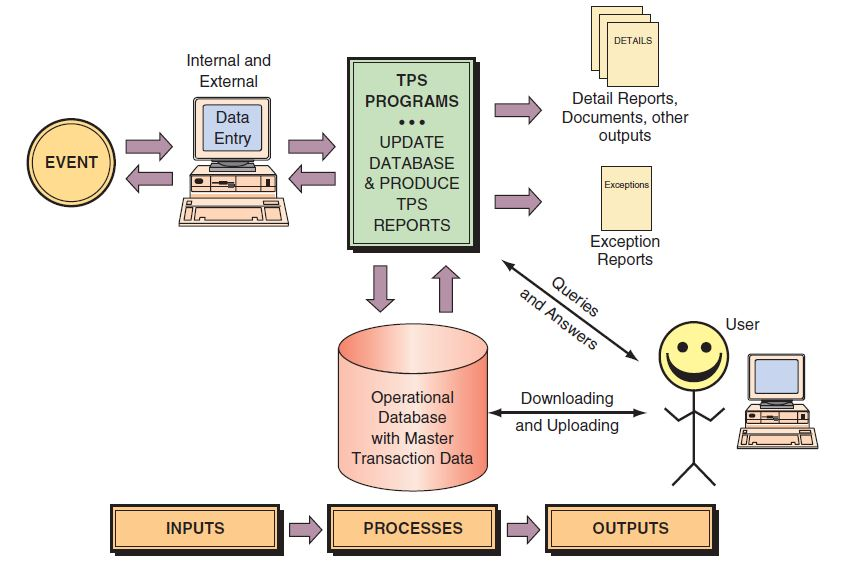
\includegraphics[scale=0.5]{F:/Skripsi/Dokumentasi_Skripsi/Gambar/Teori/tps.JPG}
		{\caption{Alur informasi pada proses transaksi} \cite{Turban:2001}}
	\label{fig:tps}
\end{figure}

\textbf{Karakteristik TPS}\\

Berikut ini akan dijelaskan karakteristik dari TPS, antara lain \cite{Turban:2001} : 
\begin{enumerate}
	\item Volume data yang diproses sangat besar.
	\item Sumber data umumnya berasal dari dalam perusahaan dan keluaran yang dihasilkan dimaksudkan untuk pihak dalam perusahaan.
	\item Pemrosesan informasi dilakukan secara teratur. Misal harian, mingguan, dan sebagainya.
	\item Dibutuhkan kapasitas penyimpan (basis data) yang besar.
	\item Dibutuhkan kecepatan pemrosesan yang tinggi karena volume data yang diolah juga besar.
	\item Umumnya sistem memantau dan mengumpulkan data yang telah di-\textit{input} sebelumnya.
	\item Jenis data masukan dan keluaran sudah terstruktur. Karena data yang diproses cukup stabil, data diformat dalam suatu standar.
	\item Level kerincian yang tinggi terutama pada masukan tetapi seringkali juga pada keluaran.
	\item Komputasi tidak rumit (menggunakan operasi matematika sederhana atau operasi statistik).
	\item Dibutuhkan tingkat akurasi, integrasi dan keamanan data yang tinggi.
	\item Dibutuhkan tingkat keandalan yang tinggi.
	\item Pengaturan terhadap permintaan merupakan suatu hal wajib. TPS memungkinkan pengguna untuk melakukan \textit{query} terhadap basis data.
\end{enumerate}

\textbf{Contoh Aplikasi TPS}\\
Berikut ini akan dijelaskan aplikasi-aplikasi apa saja yang memanfaatkan sistem informasi berbentuk TPS berdasarkan fungsinya, yaitu \cite{Laudon:2011} :
\begin{enumerate}
	\item Sistem pemasaran (\textit{Sales})
	\item Sistem produksi (\textit{Manufacturing})
	\item Sistem akuntansi (\textit{Finance})
	\item Sistem ketenaga kerjaan (\textit{HR})
	\item Lain-lain (contoh : universitas)
\end{enumerate}

\subsection{\textit{Office Automation System} (OAS)}
\label{sec:oas}
\textit{Office Automation System} (OAS) adalah aplikasi yang didesain untuk meningkatkan produktivitas pegawai di kantor dengan mendukung koordinasi dan komunikasi antar pegawai \cite{Susan:1982}. OAS digunakan untuk meningkatkan aliran pekerjaan dan komunikasi antar sesama pegawai, tidak peduli apakah pekerja tadi berada di satu lokasi yang sama ataupun tidak sehingga tingkat produktivitas pegawai dapat meningkat.

\textbf{Dampak dari Otomatisasi}\\
Otomatisasi proses dapat membawa dampak positif pada organisasi yang menerapkannya. Dampak dari otomatisasi terbagi menjadi 3 tingkatan yaitu \cite{Susan:1982}: 
\begin{enumerate}
	\item \textit{Innovative}\\
	Tingkat ini merupakan tahap awal dari otomatisasi. Pada level ini organisasi mulai menerapkan metode baru, penggunaan \textit{tools} dan teknik dalam pengerjaan beberapa tugasnya. Dampak otomatisasi pada level ini ditandai dengan tumbuhnya dan berkembangannya sektor bisnis.
	\item \textit{Rective}\\
	Tingkat ini organisasi mulai meningkatkan dukungan dan fasilitas untuk para manajer dan pegawai, kontorl sistem yang lebih baik dari sebelumnya dan semakin mudahnya mengakses suatu informasi yang akurat. Dampaknya produktivitas pegawai akan meningkat.
	\item \textit{Routine}\\
	Tingkat ini merupakan level teratas dari otomatisasi proses. Pada level ini hampir semua tugas yang ada pada organisasi sudah sebagian besar diotomatisasi. Dampaknya akan terasa pada berkurangnya biaya produksi dan peningkatan pada muatan pekerjaan dari staf pendukung.
\end{enumerate}
 
\section{\LaTeX}
\label{sec:latex}
\LaTeX adalah sebuah bahasa \textit{markup} untuk sistem penulisan dokumen yang dikembangkan oleh Leslie B. Lamport dan dirilis pada tahun 1985 \cite{Lamport:1994}. \LaTeX memiliki filosofi WYMIWYG (\textit{What You Mean Is What You Get}) yang berarti sesuatu yang akan kita tulis akan ditulis berdasarkan arti dari hal tersebut. Oleh karena itu, untuk menambahkan suatu perintah pada dokumen yang sedang kita tulis perlu menambahkan suatu \textit{command}. \textit{Command} adalah kata spesial yang menentukan suatu sifat pada \LaTeX. Hampir semua \textit{command} pada \LaTeX selalu diawali dengan tanda '\textbackslash' dan beberapa \textit{command} memiliki \textit{parameter}. \textit{Parameter} diawali dengan tanda kurung kurawal buka dan diakhiri denga kurung kurawal tutup(\{\}). \textit{File} \LaTeX memiliki ekstensi .tex.  

Untuk menulis dokumen pada \LaTeX dibutuhkan beberapa \textit{command} yang wajib ada dalam sebuah dokumen, yaitu \cite{Lamport:1994} : 
\begin{enumerate}
	\item \texttt{\string\documentclass[option]\{class\}}\\
	Digunakan untuk menentukan jenis dokumen dan \textit{layout} dokumen. Bagian \textit{option} dapat dikosongkan atau dapat digunakan untuk menyimpan pilihan pengaturan \textit{layouting}. Pada bagian \textit{class} digunakan untuk menentukan tipe dokumen yang akan dibuat.
	\item \texttt{\string\usepackage\{package name\}}\\
	Digunakan untuk menambahkan sebuah \textit{package} baru untuk mendukung pembuatan dokumen. Package adalah sebuah pengaturan yang berisi sekumpulan \textit{command} dan pengaturan yang akan digunakan untuk mengatur keseluruhan isi dokumen. \textit{Package name} diisi dengan nama \textit{package} yang akan digunakan.
	\item \texttt{\string\title\{\}}\\
	Digunakan untuk menapilkan halaman judul. Biasanya halaman judul akan memuat judul dokumen, nama pengarang dan tanggal pembuatan dokumen. Nama pengarang dan tanggal pembuatan dapat ditampilkan dengan menambahkan perintah \texttt{\string\author\{nama\}} dan \texttt{\string\date\{tanggal\}}
	\item \texttt{\string\begin\{document\}}...\texttt{\string\end\{document\}}\\
	Digunakan untuk mengawali dan mengakhiri isi dokumen.
\end{enumerate}

\subsection{Mailmerge}
\label{sec:mailmerge}
\textit{Mailmerge} adalah salah satu \textit{package} yang disediakan oleh \LaTeX yang berupa antar muka untuk pembuatan surat atau dokumen. \textit{Mailmerge} memilik 2 komponen utama yaitu \textit{repeated text} yaitu sejumlah tulisan dalam dokumen tersebut yang ditulis sama persis berulang kali pada setiap pengulangan, dan \textit{command} yang dapat diganti-ganti dengan suatu nilai tertentu pada setiap pengulangan \cite{Frasson:2009} .\

Untuk menggunakan \textit{package mailmerge}, ada beberapa \textit{command} yang perlu ditambahkan seperti \cite{Frasson:2009} :
\begin{enumerate}
	\item \texttt{\string\mailfields}\\
	Digunakan untuk menyatakan nama \textit{field} yang akan digunakan. Nama \textit{field} disimpan di dalam \textit{parameter} \texttt{\string\mailfields}. Urutan nama \textit{field} yang dideklarasikan akan berpengaruh pada \texttt{\string\mailentry}. Nama \textit{field} akan menjadi \textit{parameter} bagi \textit{command} \texttt{\string\field}.
	\item \texttt{\string\mailrepeat}\\
	Digunakan untuk menentukan teks mana saja yag diulang setiap kali pengulangan. Teks yang akan diulang maupun \textit{command} \texttt{\string\field} akan menjadi parameter bagi \texttt{\string\mailrepeat}, namun isi dari \textit{command} \texttt{\string\field} akan berubah pada setiap kali pengulangan sesuai dengan data pada \textit{entry}.
	\item \texttt{\string\field}\\
	Digunakan untuk menempatkan nama \textit{field} pada \textit{repeated text}. Nama field disimpan di dalam \textit{parameter} \texttt{\string\field}.
	\item \texttt{\string\mailentry}\\
	Digunakan untuk penampungan nilai sebelum dimasukkan sebagai \textit{parameter} \textit{command} \texttt{\string\field}.
\end{enumerate}
	Berikut ini adalah urutan tata letak setiap \textit{command} untuk pembuatan \textit{mailmerge} :
	\begin{lstlisting}[language=tex,basicstyle=\tiny,caption=Contoh pembuatan \textit{mailmerge}]
	\documentclass[12pt]{letter}
    \usepackage{ifthen,mailmerge}

    % \ifequal{A}{B}{what if A=B}{what if A<>B}
    \newcommand{\ifequal}[2]{\ifthenelse{\equal{#1}{#2}}}

    \mailfields{name,friends,drives}

    \mailrepeat{\section*{\field{name}'s profile}

       \field{name} has
       \ifequal{\field{friends}}{}
         {no friends}
         {\field{friends} as friends}.
       \ifequal{\field{drives}}{yes}{Drives.}{Doesn't drive.}

    (entry \entrynumber\ of \numberofentries)

    % \newpage optional
    }

    \mailentry{John,{Bart and Robert},yes}
    \mailentry{Sara,{Jean, Phillip and Maria},no}
    \mailentry{Edward,,yes}
 \end{lstlisting}
 
\section{Laravel}
\label{sec:laravel}
Laravel adalah \textit{framework web} berbasis php yang bersifat \textit{open-source} yang dikembangkan oleh Taylor Otwell pada Juni 2011\cite{surguy:2013}. Laravel menerapkan pola arsitektur \textit{Model-View-Controller} (MVC) dimana \textit{layer} memiliki fungsi yang berbeda-beda.

\subsection{Komponen Utama Laravel}
\label{sec:komponen_utama_laravel}
Laravel memiliki beberapa \textit{file} yang menjadi komponen utama yang perlu diperhatikan. \textit{File-file} tersebut yaitu\cite{laravel:2016} :
\begin{itemize}
	\item \textit{Model}\\
	\textit{Model} merupakan bagian yang menghubungkan antara aplikasi dengan \textit{database}.
	\item \textit{View}\\
	\textit{View} merupakan bagian yang bertugas menampilkan \textit{file} tampilan ke pengguna.  
	\item \textit{Controller}\\
	\textit{Controller} bertugas menjalankan proses lojik dan juga menerima \textit{input request} dari \textit{view}.
	\item \textit{Route}\\
	\textit{Route} bertugas mengatur pemetaan jalur \textit{request} dari \textit{view} ke \textit{controller}.  
\end{itemize}}{}
\ifdefstring{\vbabc}{1}{\chapter{Analisis}
\label{chap:analisis}
Pada analisis membahas mengenai deskripsi sistem terkini dan analisis sistem usulan.

\section{Deskripsi Sistem Terkini}
\label{sec:deskripsi_sistem_terkini}
Deskripsi sistem terkini membahas mengenai gambaran umum institusi, jenis-jenis surat akademik yang dikeluarkan oleh pihak TU, prosedur pemesanan surat akademik, prosedur pembuatan surat akademik, prosedur pengambilan surat akademik dan analisis kebutuhan. \\

\subsection{Gambaran Umum Institusi}
\label{sec:gambaran_umum_institusi}
Fakultas Teknologi Informasi dan Sains (FTIS) adalah salah satu fakultas yang terdapat di kampus Universitas Katolik Parahyangan (UNPAR). FTIS dikepalai oleh seorang dekan yang dibantu oleh 3 wakil dekan. FTIS memiliki 3 program studi (prodi) yaitu Prodi Matematika, Fisika dan Teknik Informatika. Setiap prodi dipimpin oleh seorang ketua prodi yang dibantu oleh seorang sekretaris prodi, kecuali Prodi Fisika. Setiap prodi, kecuali Prodi Matematika, memiliki laboratorium yang dikepalai oleh seorang kepala laboratorium. Untuk mengurusi masalah administrasi fakultas, terdapat bagian Tata Usaha (TU) yang terdiri dari sub bagian (subag) tertentu yang mengurusi bidang tertentu.\

Gambar \hyperlink{organigram_fakultas}{3.1} menjelaskan struktur organisasi dari FTIS. Di bawah ini akan dijelaskan  setiap bagian dari struktur organisasi tersebut. Setiap fungsi pada struktur organisasi tersebut memiliki tugas, wewenang, dan tanggung jawab yang berbeda.
\begin{figure}[H]
	\centering
		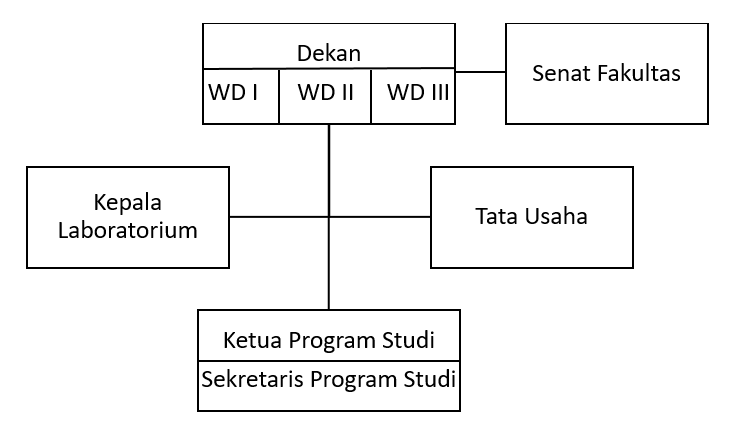
\includegraphics[scale=0.45]{F:/Skripsi/Dokumentasi_Skripsi/Gambar/Diagram/sistem_terkini/organigram/organigram_fakultas_new.PNG}
	\caption{Struktur organisasi Fakultas Teknologi Informasi dan Sains}
	\label{fig:organigram_fakultas}
\end{figure}

\begin{enumerate}
	\item Dekan \\
	berfungsi sebagai pengambil keputusan tertinggi di fakultas.
	\item Senat Fakultas \\
	berfungsi sebagai partner dekan untuk membantu memberikan pertimbangan dari keputusan yang akan diambil. Senat dipilih dari dosen tetap di fakultas.
	\item Wakil Dekan Bidang Akademik (WD I)\\
	berfungsi untuk membantu dekan pada pengambilan segala keputusan yang berhubungan dengan kegiatan akademik yang berlangsung di setiap program studi yang ada pada fakultas.
	\item Wakil Dekan Bidang Sumber Daya (WD II)\\
	berfungsi untuk membantu dekan pada pengambilan segala keputusan yang berhubungan dengan pengelolaan setiap bentuk sumber daya yang terdapat di lingkungan fakultas.
	\item Wakil Dekan Bidang Kemahasiswaan dan Alumni (WD III)\\
	berfungsi untuk membantu dekan pada pengambilan segala keputusan yang berhubungan dengan setiap permasalahan kemahasiswaan dan alumni di lingkungan fakultas.
	\item Kepala Laboratorium \\
	bertanggung jawab akan perawatan dan operasional laboratorium.
	\item Ketua Program Studi \\
	berfungsi sebagai pengambil keputusan tertinggi di lingkungan program studi.
	\item Sekretaris Program Studi \\
	berfungsi untuk membantu ketua program studi pada pengambilan segala keputusan di lingkungan program studi.
	\item Tata Usaha \\
	berfungsi untuk melayani segala kegiatan administrasi yang terjadi di lingkungan FTIS.
\end{enumerate}

Gambar \hyperlink{organigram_TU}{3.2} merupakan struktur organisasi dari TU FTIS. Bagian tata usaha dipimpin oleh seorang Kepala Bagian (Kabag). Di bawah Kabag terdapat 4 sub bagian (Subag) yang dikepalai oleh seorang Kepala Sub Bagian (Kasubag). Berikut ini akan dijelaskan struktur organisasi yang ada di tata usaha FTIS.
\begin{figure}[H]
	\centering
		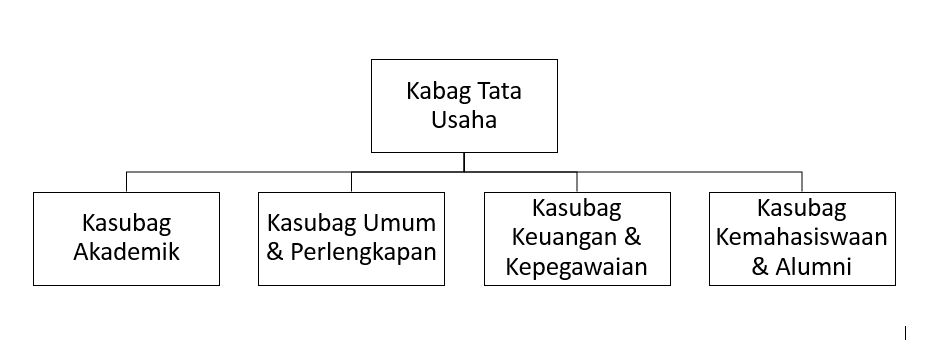
\includegraphics[scale=0.5]{F:/Skripsi/Dokumentasi_Skripsi/Gambar/Diagram/sistem_terkini/organigram/organigram_TU.JPG}
	\caption{Struktur organisasi Tata Usaha Fakultas Teknologi Informasi dan Sains}
	\label{fig:organigram_TU}
\end{figure}
\begin{enumerate}
	\item Kabag Tata Usaha \\
	berfungsi sebagai pemegang keputusan tertinggi di tata usaha.
	\item Kasubag Akademik \\
	berfungsi sebagai pengatur segala hal yang berhubungan dengan kegiatan akademik di lingkungan fakultas, seperti pengaturan jadwal kuliah dan ujian, jadwal perwalian, pembagian ruangan, memperbanyak dan mendistribusikan soal ujian, dll.
	\item Kasubag Umum dan Peralatan \\
	berfungsi sebagai pengatur segala kegiatan, sarana dan prasarana yang ada di lingkungan fakultas. 
	\item Kasubag Keuangan dan Kepegawaian \\
	berfungsi sebagai pengatur operasional keuangan dan kepegawaian di lingkungan fakultas.
	\item Kasubag Kemahasiswaan dan Alumni \\
	berfungsi untuk melayani segala keperluan kemahasiswaan dan alumni seperti keperluan surat menyurat, legalisir ijazah, mempersiapkan perlengkapan wisuda, dll.
\end{enumerate}
Berdasarkan uraian mengenai struktur organisasi fakultas, Kasubag Kemahasiswaan dan Alumni berperan mengurusi keperluan surat menyurat di fakultas. Surat-surat yang dibuat termasuk juga dengan surat akademik yang akan dibahas lebih detil pada subbab selanjutnya.

\subsection{Jenis-Jenis Surat Akademik}
\label{sec:jenis_jenis_surat_akademik}
Ada berbagai macam surat akademik yang dikeluarkan oleh TU FTIS. Surat yang dikeluarkan antara lain sebagai berikut :
\begin{enumerate}
	\item Surat keterangan beasiswa \\
	Surat ini berfungsi sebagai surat pernyataan bahwa mahasiswa yang bersangkutan telah menerima beasiswa dari pihak non-Unpar dan tidak menerima beasiswa lain yang berasal dari Unpar.

	\item Surat keterangan \\
	Surat ini memiliki fungsi yang beragam. Surat ini dapat digunakan untuk pernyataan mahasiswa aktif, pembuatan surat kelakuan baik, membuka rekening, membuat visa, dll.
	
	\item Surat izin studi lapangan \\
	Surat ini berfungsi sebagai surat pengantar apabila ada mahasiswa yang hendak melakukan wawancara, survei, studi banding atau observasi ke sebuah instansi.
	
	\item Surat izin cuti studi \\
	Surat ini berlaku apabila mahasiswa yang bersangkutan tidak akan mengikuti perkuliahan pada semester tertentu. Biasanya surat ini digunakan apabila mahasiswa mengalami sakit keras dan membutuhkan masa penyembuhan yang lama ataupun tidak ada mata kuliah yang dibuka pada semester yang berjalan. Surat ini dapat diproses apabila mahasiswa pemohon telah memenuhi 2 syarat, yaitu tidak memiliki tunggakan pembayaran uang kuliah dan sudah membayar uang cuti studi.
	
	\item Surat izin pengunduran diri mahasiswa \\
	Surat ini berfungsi sebagai surat pernyataan apabila seorang mahasiswa hendak mengundurkan diri dari Unpar. Biasanya lasan pengambilan surat ini dikarenakan mahasiswa yang bersangkutan merasa tidak cocok dengan jurusan atau telah diterima di universitas lain dan hendak berkuliah di universitas tersebut.

	\item Surat perwakilan perwalian \\
	Surat ini berlaku apabila mahasiswa yang bersangkutan berhalangan hadir untuk melakukan perwalian dengan dosen wali sehingga diwakilkan kepada mahasiswa lain yang diberi kuasa.
	
	\item Surat dispensasi pembayaran \\
	Surat ini berlaku apabila mahasiswa yang bersangkutan berencana mengambil mata kuliah kurang dari 10 SKS pada semester yang akan ditempuh. Surat ini harus diproses sebelum masa FRS berlangsung. Surat ini berbentuk formulir isian. Pertama mahasiswa harus mengisi formulir. Setelah formulir diisi sesuai dengan data yang dibutuhkan, formulir akan diteruskan kepada dosen wali dari mahasiswa yang bersangkutan melalui Petugas TU untuk mendapatkan tanda tangan dosen wali. Setelah mendapat tanda tangan dosen wali, formulir diteruskan kepada Biro Keuangan Unpar untuk mendapatkan persetujuan. Apabila disetujui, akan dikirimkan surat persetujuan kepada Petugas TU untuk mengubah jumlah tagihan pembayaran uang kuliah milik mahasiswa di situs \textit{studentportal}. Sehingga jumlah tagihan yang muncul akan sesuai dengan SKS mata kuliah yang akan diambil. 
	
	\item Surat pengajuan pengambilan kelebihan pembayaran uang kuliah (tunai) \\
	Surat ini berlaku apabila mahasiswa yang bersangkutan telah membayar uang kuliah sesuai dengan SKS mata kuliah yang diambil namun kemudian membatalkan mata kuliah yang telah diambil tersebut. Surat ini berbentuk formulir isian. Pertama mahasiswa harus mengisi formulir. Setelah formulir diisi sesuai dengan data yang dibutuhkan, formulir akan ditandatangani oleh Petugas TU. Setelah ditandatangani, formulir diteruskan kepada Biro Keuangan Unpar untuk diproses. Setelah diproses akan dikirimkan surat keterangan pengembalian uang kuliah beserta sejumlah uang kelebihan pembayaran kuliah kepada Petugas TU. Uang akan diberikan kepada mahasiswa pemohon dan surat keterangan akan disimpan di TU sebagai arsip.

	\item Surat penundaan pembayaran uang kuliah \\
	Surat ini berlaku apabila mahasiswa yang bersangkutan belum bisa membayar uang kuliah sampai tanggal yang telah ditentukan. Fungsi surat ini yaitu untuk memberikan kelonggaran waktu pembayaran uang kuliah pada mahasiswa sehingga mahasiswa yang bersangkutan akan terlepas dari denda keterlambatan pembayaran. Pertama mahasiswa harus mengisi formulir. Setelah formulir diisi sesuai dengan data yang dibutuhkan, akan dibuatkan surat yang kemudian diteruskan kepada Wakil Dekan Bidang Sumber Daya melalui Petugas TU untuk mendapatkan tanda tangan wakil dekan. Setelah mendapat tanda tangan wakil dekan, surat diteruskan kepada Biro Keuangan Unpar untuk mendapatkan persetujuan. Apabila disetujui, akan dikirimkan surat persetujuan kepada Petugas TU yang menyatakan pemberian izin kepada mahasiswa pemohon untuk menunda pembayaran uang kuliah.
	
	\item Surat permohonan beasiswa \\
	Surat ini berfungsi apabila seorang mahasiswa hendak mengajukan beasiswa kepada universitas maupun fakultas. Surat ini berbentuk formulir isian. Setelah formulir diisi sesuai dengan data yang dibutuhkan, formulir diteruskan kepada dosen wali mahasiswa pemohon untuk mendapat catatan dan tanda tangan dosen wali. Setelah itu surat akan diteruskan kepada dekan untuk catatan dan tanda tangan dekan. Setelah semua data terisi lengkap, formulir akan diserahkan kepada Badan Kemahasiswaan dan Alumni Unpar.
	\end{enumerate}

\subsection{Prosedur Pemesanan Surat}
\label{sec:prosedur_pemesanan_surat}
Gambar \hyperlink{pemesanan_terkini}{3.3} merupakan prosedur pemesanan surat yang dilakukan oleh mahasiswa kepada Kasubag Kemahasiswaan dan Alumni. Untuk selanjutnya Kasubag Kemahasiswaan dan Alumni akan disebut sebagai Petugas TU untuk mempersingkat penyebutan nama. Prosedur pemesanan surat dimulai dengan:
\begin{enumerate}
	\item Mahasiswa mendatangi Petugas TU dan menyebutkan surat yang dibutuhkan
	\item Petugas TU memberikan formulir yang harus diisi sesuai dengan surat yang dibutuhkan
	\item Mahasiswa mengisi formulir
	\item Mahasiswa mengembalikan formulir ke Petugas TU
	\item Petugas TU mengecek pengisian formulir. Apabila ada kesalahan pengisian, maka formulir dikembalikan kepada mahasiswa untuk diperbaiki. Jika tidak ada kesalahan maka dapat lanjut ke proses berikutnya
	\item Apabila sedang tidak ada pesanan surat, surat dapat langsung dibuatkan, apabila ada pesanan, surat akan masuk \textit{waiting list} dan Petugas TU akan memberikan estimasi waktu selesai pengerjaan surat
\end{enumerate}

\begin{figure}[H]
	\centering
		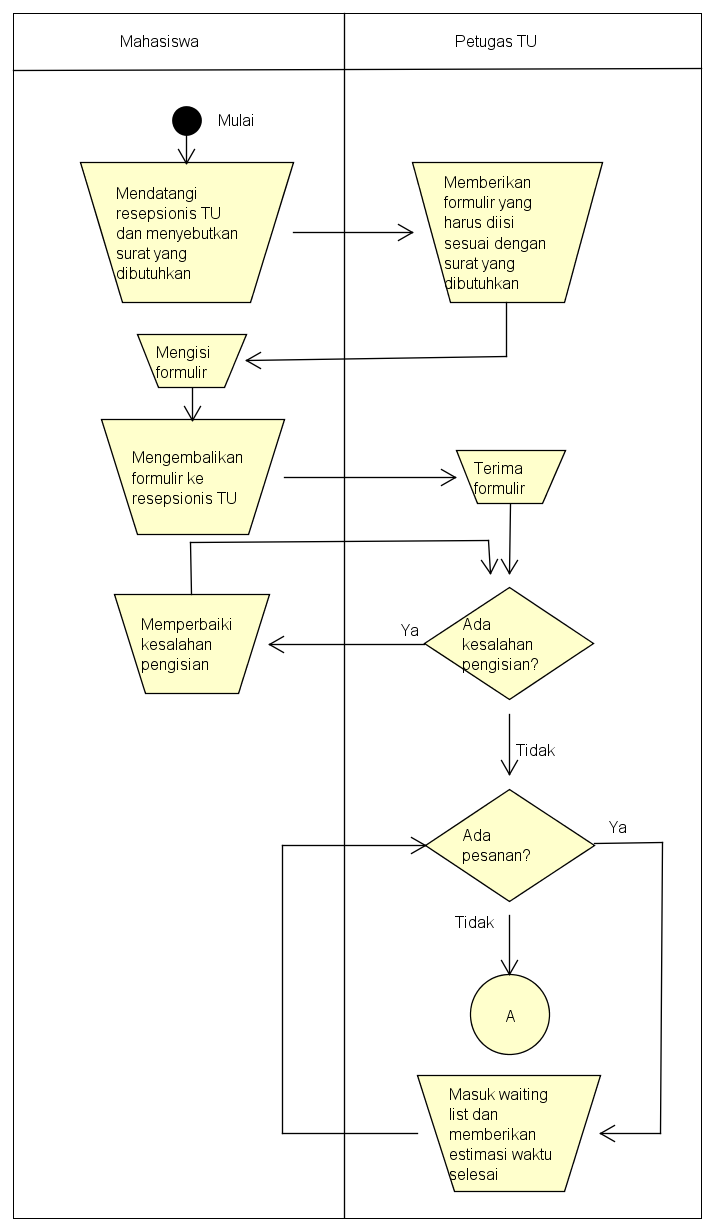
\includegraphics[scale=0.7]{F:/Skripsi/Dokumentasi_Skripsi/Gambar/Diagram/sistem_terkini/work_flow/pemesanan_terkini.png}
	{\caption{Prosedur pemesanan surat terkini}}
	\label{fig:pemesanan_terkini}
\end{figure}

\subsection{Prosedur Pembuatan Surat}
\label{sec:prosedur_pembuatan_surat}
Gambar \hyperlink{pembuatan_terkini}{3.4} merupakan prosedur pembuatan surat yang dilakukan oleh Petugas TU. Prosedur pembuatan surat dimulai dengan:
\begin{enumerate}
	\item Petugas TU mengecek formulir yang telah diisi oleh mahasiswa
	\item Petugas TU membuka \textit{template} surat yang dipesan
	\item Petugas TU memasukkan semua data yang telah dituliskan oleh mahasiswa pada formulir ke \textit{template}
	\item Petugas TU melakukan cek ulang apabila terjadi kesalahan dalam memasukkan data
	\item Apabila tidak ada kesalahan Petugas TU dapat langsung mencetak surat
	\item Petugas akan menghubungi pejabat tertentu yang memiliki keterkaitan dengan surat yang sedang diproses untuk mendapatkan tanda tangan dari pejabat yang bersangkutan
	\item Apabila mahasiswa pemohon menunggu di sekitar ruang TU maka surat dapat langsung diambil oleh mahasiswa pemohon. Apabila tidak ada, maka surat akan disimpan oleh Petugas TU
\end{enumerate}

\begin{figure}[H]
	\centering
		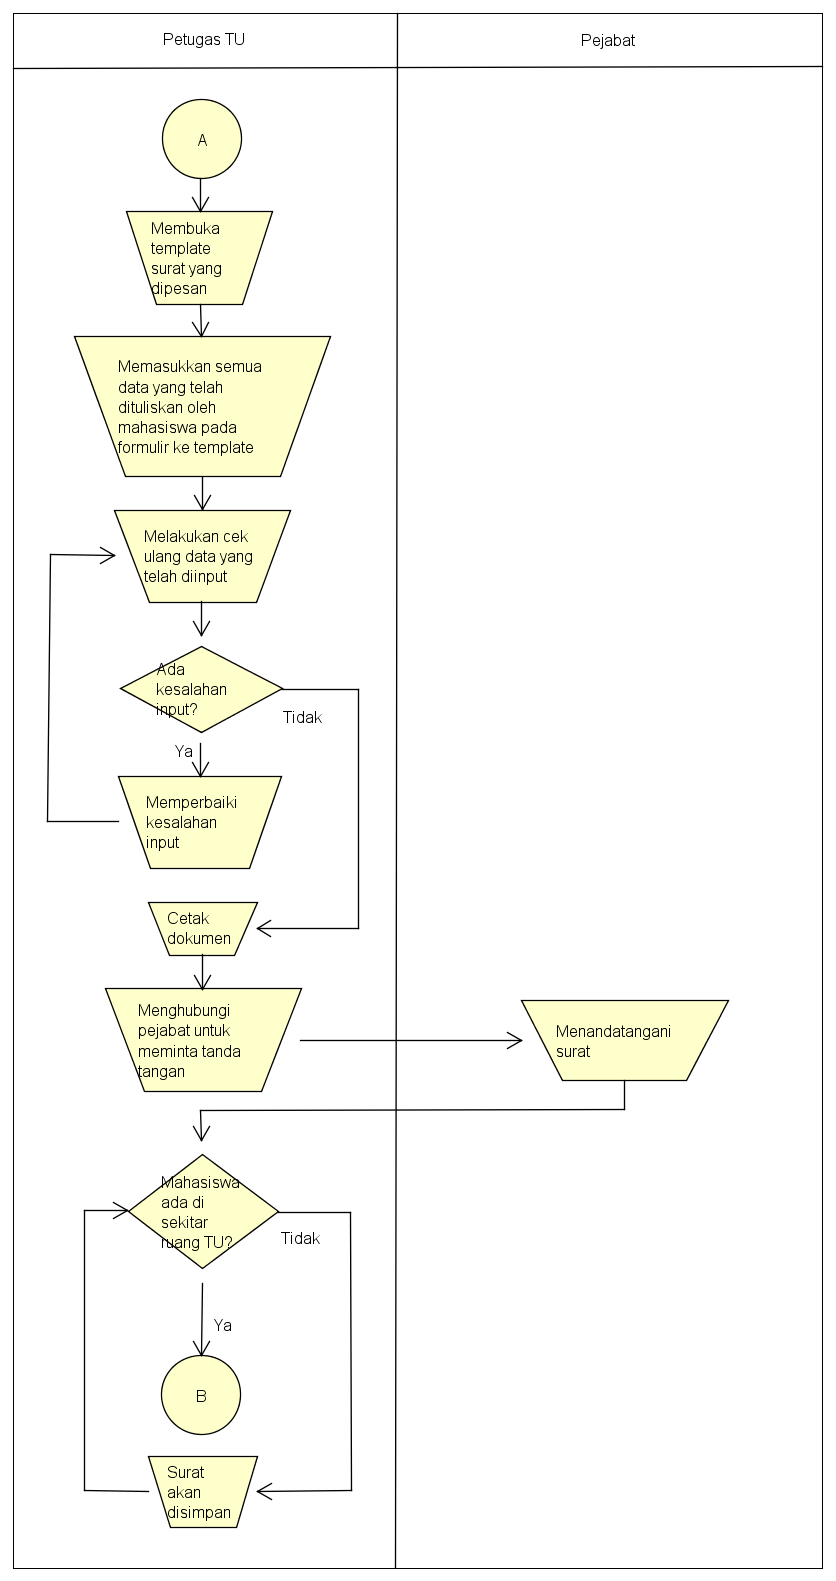
\includegraphics[scale=0.6]{F:/Skripsi/Dokumentasi_Skripsi/Gambar/Diagram/sistem_terkini/work_flow/pembuatan_terkini.png}
	{\caption{Prosedur pembuatan surat terkini}}
	\label{fig:pembuatan_terkini}
\end{figure}

\subsection{Prosedur Pengambilan Surat}
\label{sec:prosedur_pengambilan_surat}
Gambar \hyperlink{pengambilan_terkini}{3.5} merupakan prosedur pengambilan surat yang dilakukan oleh mahasiswa kepada Petugas TU. Prosedur pengambilan surat dimulai dengan:
\begin{enumerate}
	\item Mahasiswa yang memesan mendatangi Petugas TU dan menyebutkan surat apa yang telah dipesan
	\item Petugas TU memberikan surat yang telah dicetak kepada mahasiswa
\end{enumerate}

\begin{figure}[H]
	\centering
		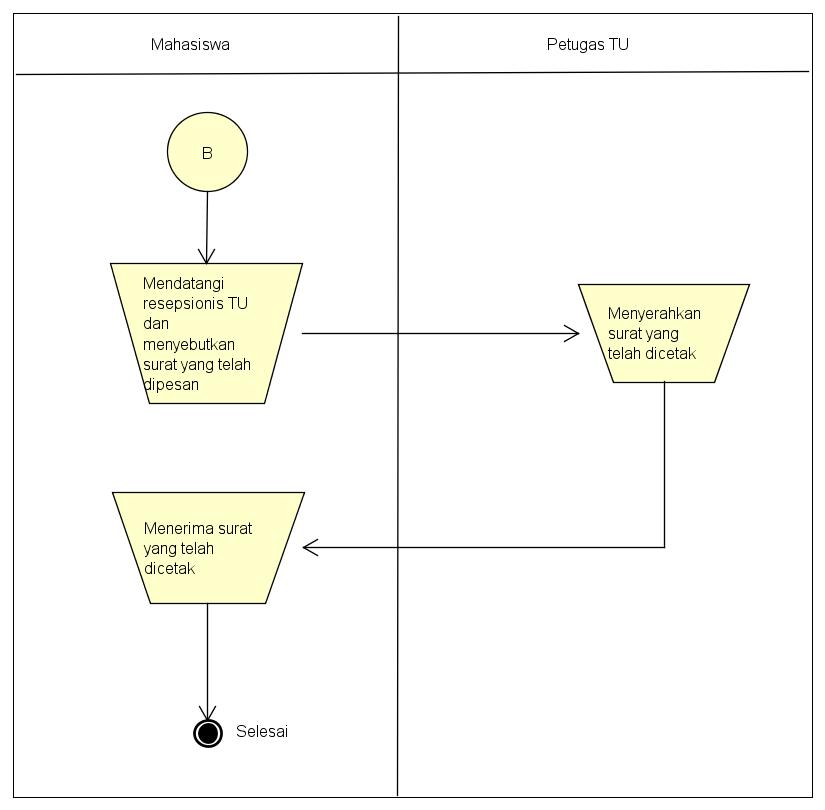
\includegraphics[scale=0.5]{F:/Skripsi/Dokumentasi_Skripsi/Gambar/Diagram/sistem_terkini/work_flow/pengambilan_terkini.jpg}
	{\caption{Prosedur pengambilan surat terkini}}
	\label{fig:pengambilan_terkini}
\end{figure}

\subsection{Analisis Kebutuhan}
\label{sec:analisis_kebutuhan}
Berdasarkan paparan yang telah disebutkan di atas, maka ditemukan beberapa masalah yang menjadi fokus utama dari penelitian ini. Masalah-masalah yang telah ditemukan antara lain:
\begin{enumerate}
	\item Pemesanan surat akademik tidak bisa dilakukan mendadak.
	\item Petugas bisa kewalahan apabila permintaan surat yang masuk cukup banyak dalam sehari.
	\item Ada kemungkinan kesalahan pemasukan data dari formulir ke komputer.
\end{enumerate}

\section{Analisis Sistem Usulan}
\label{sec:analisis_sistem_usulan}
Analisis sistem usulan membahas mengenai surat-surat yang ditangani, prosedur pembuatan surat usulan, \textit{Data Flow Diagram} (DFD), analisis kebutuhan data surat, dan diagram ER. \\

\subsection{Surat-surat yang Ditangani}
\label{sec:surat_yang_ditangani}
Dari 10 surat yang telah disebutkan di atas, diambil 6 surat yang akan dibahas lebih lanjut pada penelitian ini. Hal ini dikarenakan 6 surat tersebut dapat menghasilkan surat yang kemudian akan dikembalikan kepada mahasiswa yang bersangkutan untuk kemudian disampaikan kepada lembaga yang membutuhkan surat tersebut. Dari keenam surat tersebut ada satu surat yang memiliki fungsi ganda yaitu surat keterangan sehingga dibuat menjadi 2 jenis surat yang berbeda sehingga total terdapat 7 surat yang akan dibahas. Ketujuh surat tersebut yaitu :
\begin{enumerate}
	\item Surat keterangan beasiswa \\
	Surat pernyataan bahwa mahasiswa ybs. tidak menerima beasiswa dari pihak universitas maupun fakultas dan hanya menerima beasiswa dari satu organisasi/perusahaan saja.
	\item Surat keterangan mahasiswa aktif \\
	Surat pernyataan bahwa mahasiswa ybs. merupakan mahasiswa aktif Fakultas Teknologi Informasi dan Sains Uiversitas Katolik Parahyangan.
	\item Surat pengantar pembuatan visa \\
	Surat yang pengantar yang diajukan mahasiswa kepada suatu kedutaan besar negara asing dengan tujuan untuk untuk membuat visa.
	\item Surat izin studi lapangan \\
	Surat izin yang diajukan apabila seorang mahasiswa hendak melakukan penelitian ke suatu organisasi dan membutuhkan surat pengantar dari fakultas sebagai syarat penelitian. Surat ini dapat digunakan untuk perorangan maupun kelompok. Untuk surat izin studi lapangan kelompok, dapat mewakili 1 orang ketua dan maksimal 4 orang anggota.
	\item Surat perwalian yang diwakilkan \\
	Surat yang diajukan oleh mahasiswa apabila mahasiswa ybs. berhalangan hadir pada saat perwalian dan hendak diwakilkan oleh mahasiswa lain. 
	\item Surat izin cuti studi \\
	Surat yang diajukan oleh mahasiswa apabila mahasiswa ybs. hendak mengambil cuti studi pada semester tertentu. Surat ini memerlukan lampiran dari orang tua/wali untuk
	\item Surat izin pengunduran diri mahasiswa \\
	Surat yang diajukan oleh mahasiswa apabila mahasiswa ybs. hendak mengundurkan diri dari Fakultas Teknologi Informasi dan Sains Universitas Katolik Parahyangan.
\end{enumerate}

\subsection{Prosedur Pembuatan Surat Usulan}
\label{sec:pembuatan_surat_usulan}
Gambar \hyperlink{pembuatan_usulan}{3.6} merupakan prosedur pembuatan surat yang dilakukan oleh mahasiswa. Pada prosedur usulan ini, untuk membuat surat akademik tidak perlu melalui 3 tahapan seperti yang dijelaskan pada subbagian sistem terkini. Prosedur pembuatan surat dimulai dengan:
\begin{enumerate}
	\item Mahasiswa melakukan login
	\item Mahasiswa memilih kategori surat yang akan dibuat
	\item Mahasiswa memilih jenis surat yang akan dibuat
	\item Mahasiswa memasukkan data yang dibutuhkan dengan benar
	\item Mahasiswa menekan tombol \textit{preview} untuk melihat surat secara keseluruhan
	\item Apabila terdapat kesalahan pada pengisian data, mahasiswa dapat mengklik tombol "Kembali" untuk memperbaiki kesalahan pada pengisian data.
	\item Apabila tidak ada kesalahan, mahasiswa dapat menekan tombol "Buat Surat" untuk memesan surat tersebut dan surat akan masuk ke \textit{database} pesanan surat.
	\item Apabila \textit{id} surat adalah 9 atau 10, surat perlu melalui tahap persetujuan dari Pejabat. Sedangkan surat dengan \textit{id} 1-9 atau 11-20 maka surat dapat langsung diberi nomor surat.
	\item Setelah surat diberi nomor surat, surat dapat di-\textit{generate} menjadi \textit{file} PDF dan surat siap untuk dicetak.	
	\item Setelah surat dicetak, surat akan ditandatangani oleh Pejabat yang berwenang menandatangani surat tersebut. Apabila surat sudah ditandatangani, Pejabat akan mengubah status penandatanganan surat dari "Belum" menjadi "Sudah".
	\item Setelah surat ditandatangani, Petugas TU mengembalikan surat yang sudah ditanda tangani tersebut kepada mahasiswa. Apabila surat sudah diambil oleh mahasiswa pemohon, Petugas TU akan mengubah status pengambilan surat dari "Belum" menjadi "Sudah".
	\
\end{enumerate}
\begin{figure}[H]
	\centering
		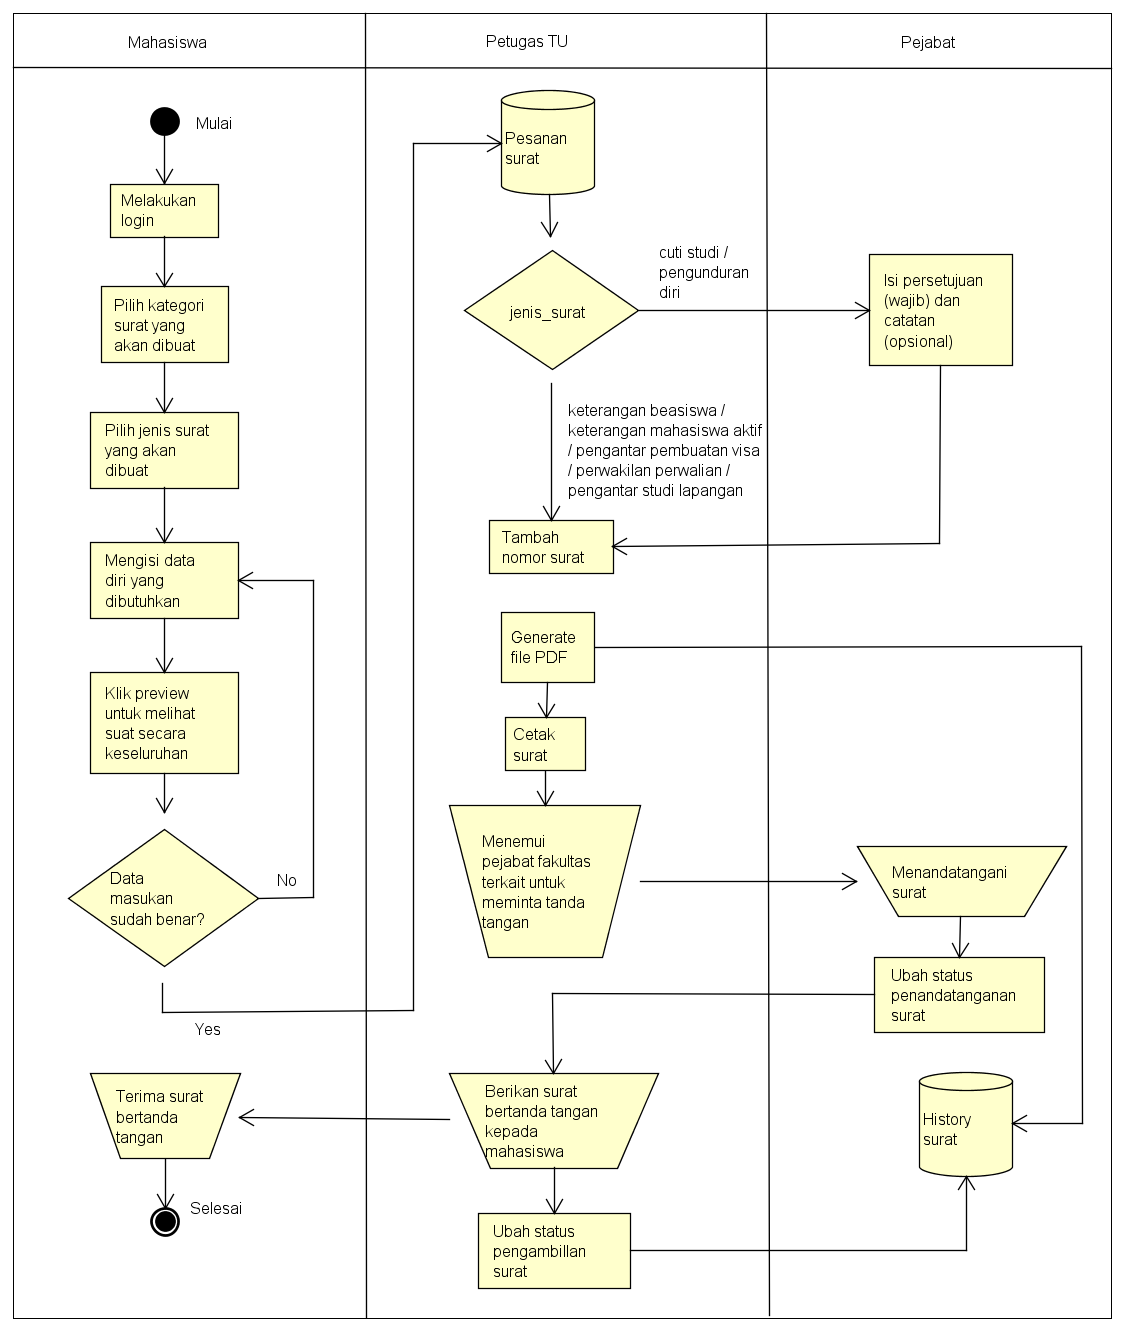
\includegraphics[scale = 0.5]{F:/Skripsi/Dokumentasi_Skripsi/Gambar/Diagram/sistem_usulan/flowchart/Flowchartsmaller.png}
	{\caption{Prosedur pembuatan surat usulan}}
	\label{fig:pembuatan_usulan}
\end{figure}

\subsection{\textit{Data Flow Diagram (DFD)}}
\label{sec:data_flow_diagram}
\textit{Data Flow Diagram (DFD)} adalah diagram untuk memodelkan setiap aliran data pada sistem yang akan dibangun.
Gambar \hyperlink{data_flow}{3.7} merupakan diagram \textit{context} atau DFD \textit{level} 0 yang menjelaskan 
keseluruhan sistem beserta aktornya.

\begin{figure}[H]
	\centering
		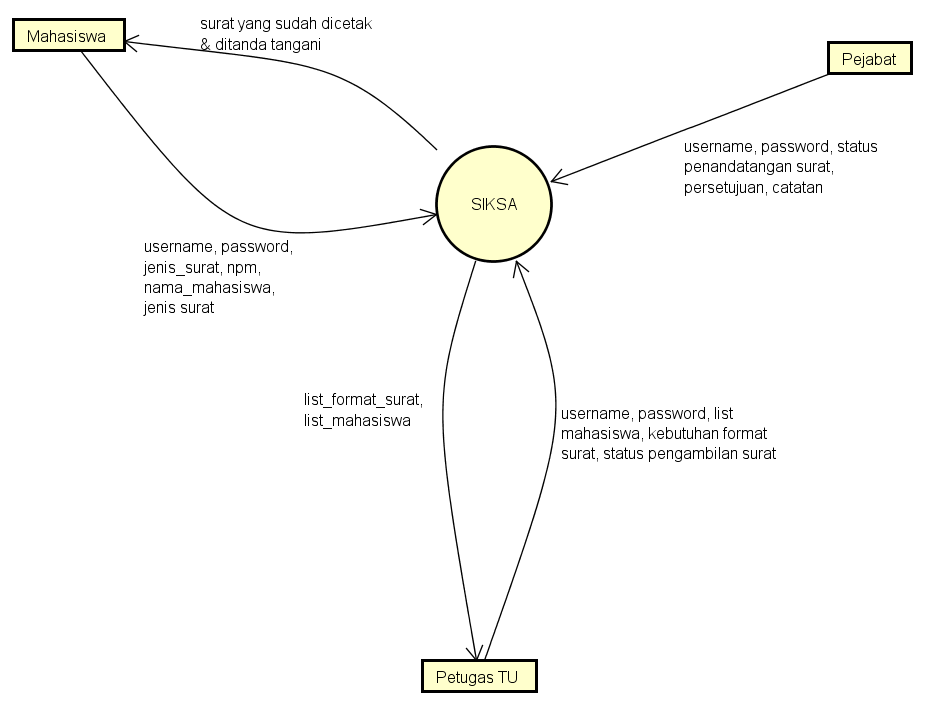
\includegraphics[scale = 0.6]{F:/Skripsi/Dokumentasi_Skripsi/Gambar/Diagram/sistem_usulan/dfd/Lv0.png}
	\caption{Diagram \textit{context}}
	\label{fig:data_flow}
\end{figure}

\textit{Website} penyedia surat akademik ini memiliki 3 aktor, yaitu \textit{mahasiswa}, \textit{pejabat} dan \textit{petugas TU}. Tiap aktor memiliki hak akses ke beberapa fitur tertentu. Gambar \hyperlink{level_1}{3.8} merupakan DFD \textit{level} 1 yang menjelaskan aliran data pada tiap aktor.

\begin{figure}[H]
	\centering
		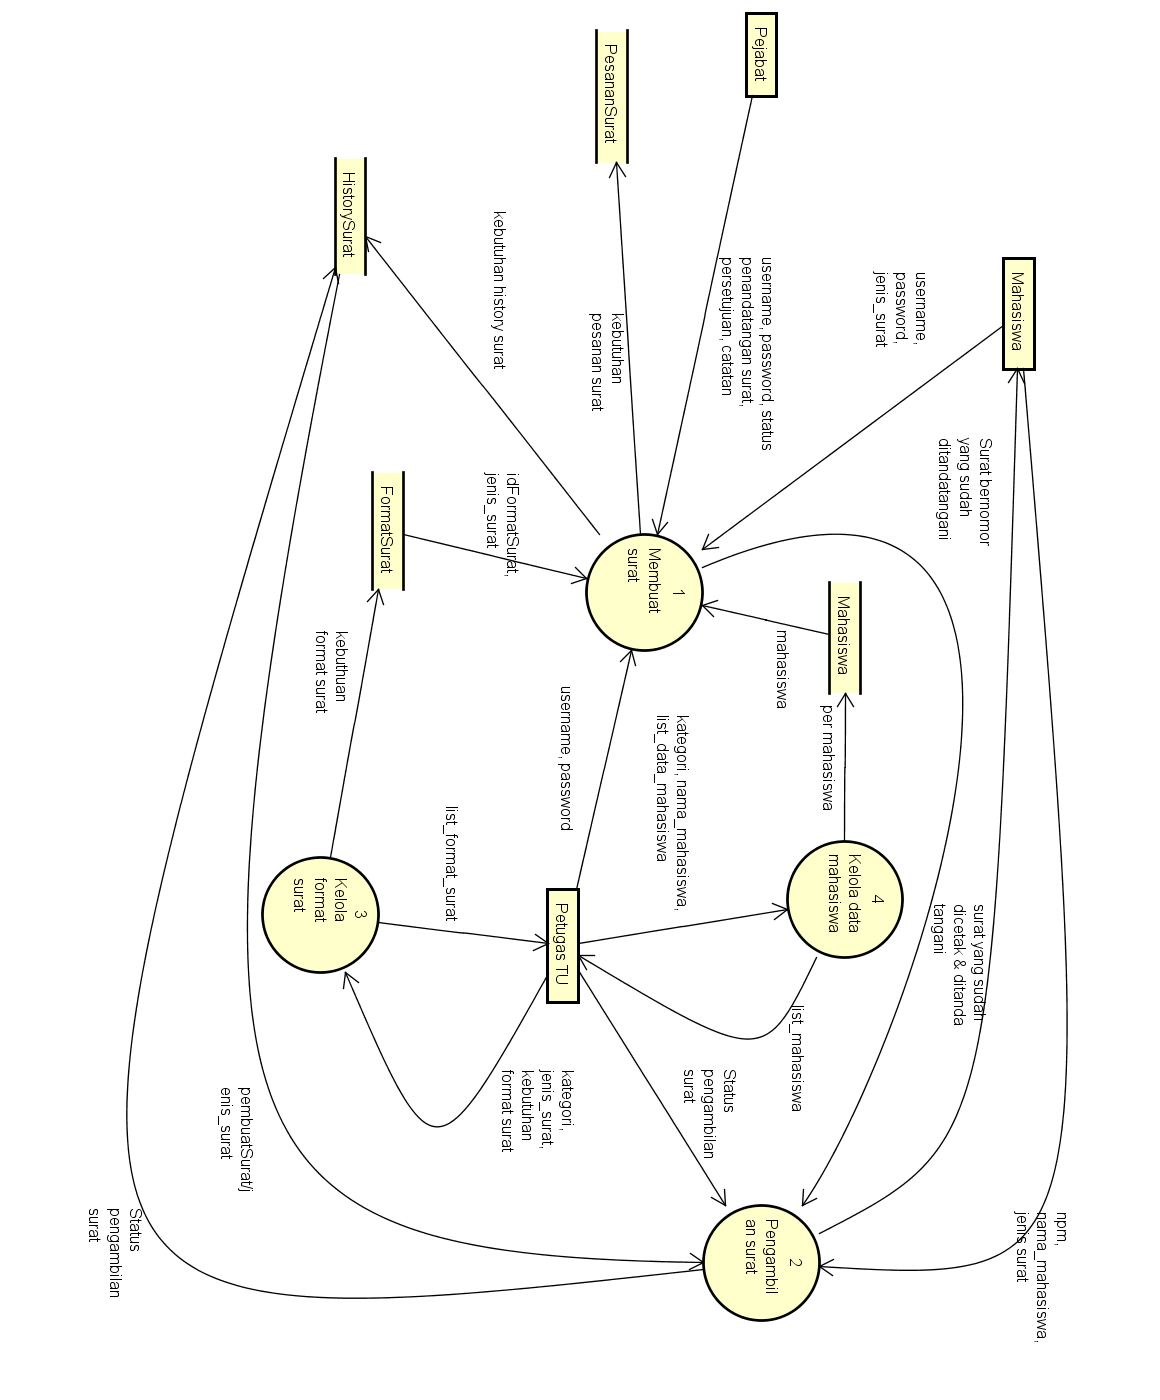
\includegraphics[scale = 0.5]{F:/Skripsi/Dokumentasi_Skripsi/Gambar/Diagram/sistem_usulan/dfd/Lv1-kiri.png}
	\caption{DFD \textit{level} 1}
	\label{fig:level_1}
\end{figure}

Gambar \hyperlink{level_2-1}{3.9} merupakan DFD \textit{level} 2-1 yang menjelaskan aliran data pada saat aktor mahasiswa hendak membuat surat yang kemudian dilanjutkan pada DFD \textit{level} 3-1.10 pada gambar \hyperlink{level_3-1.10}{3.10}

\begin{figure}[H]
	\centering
		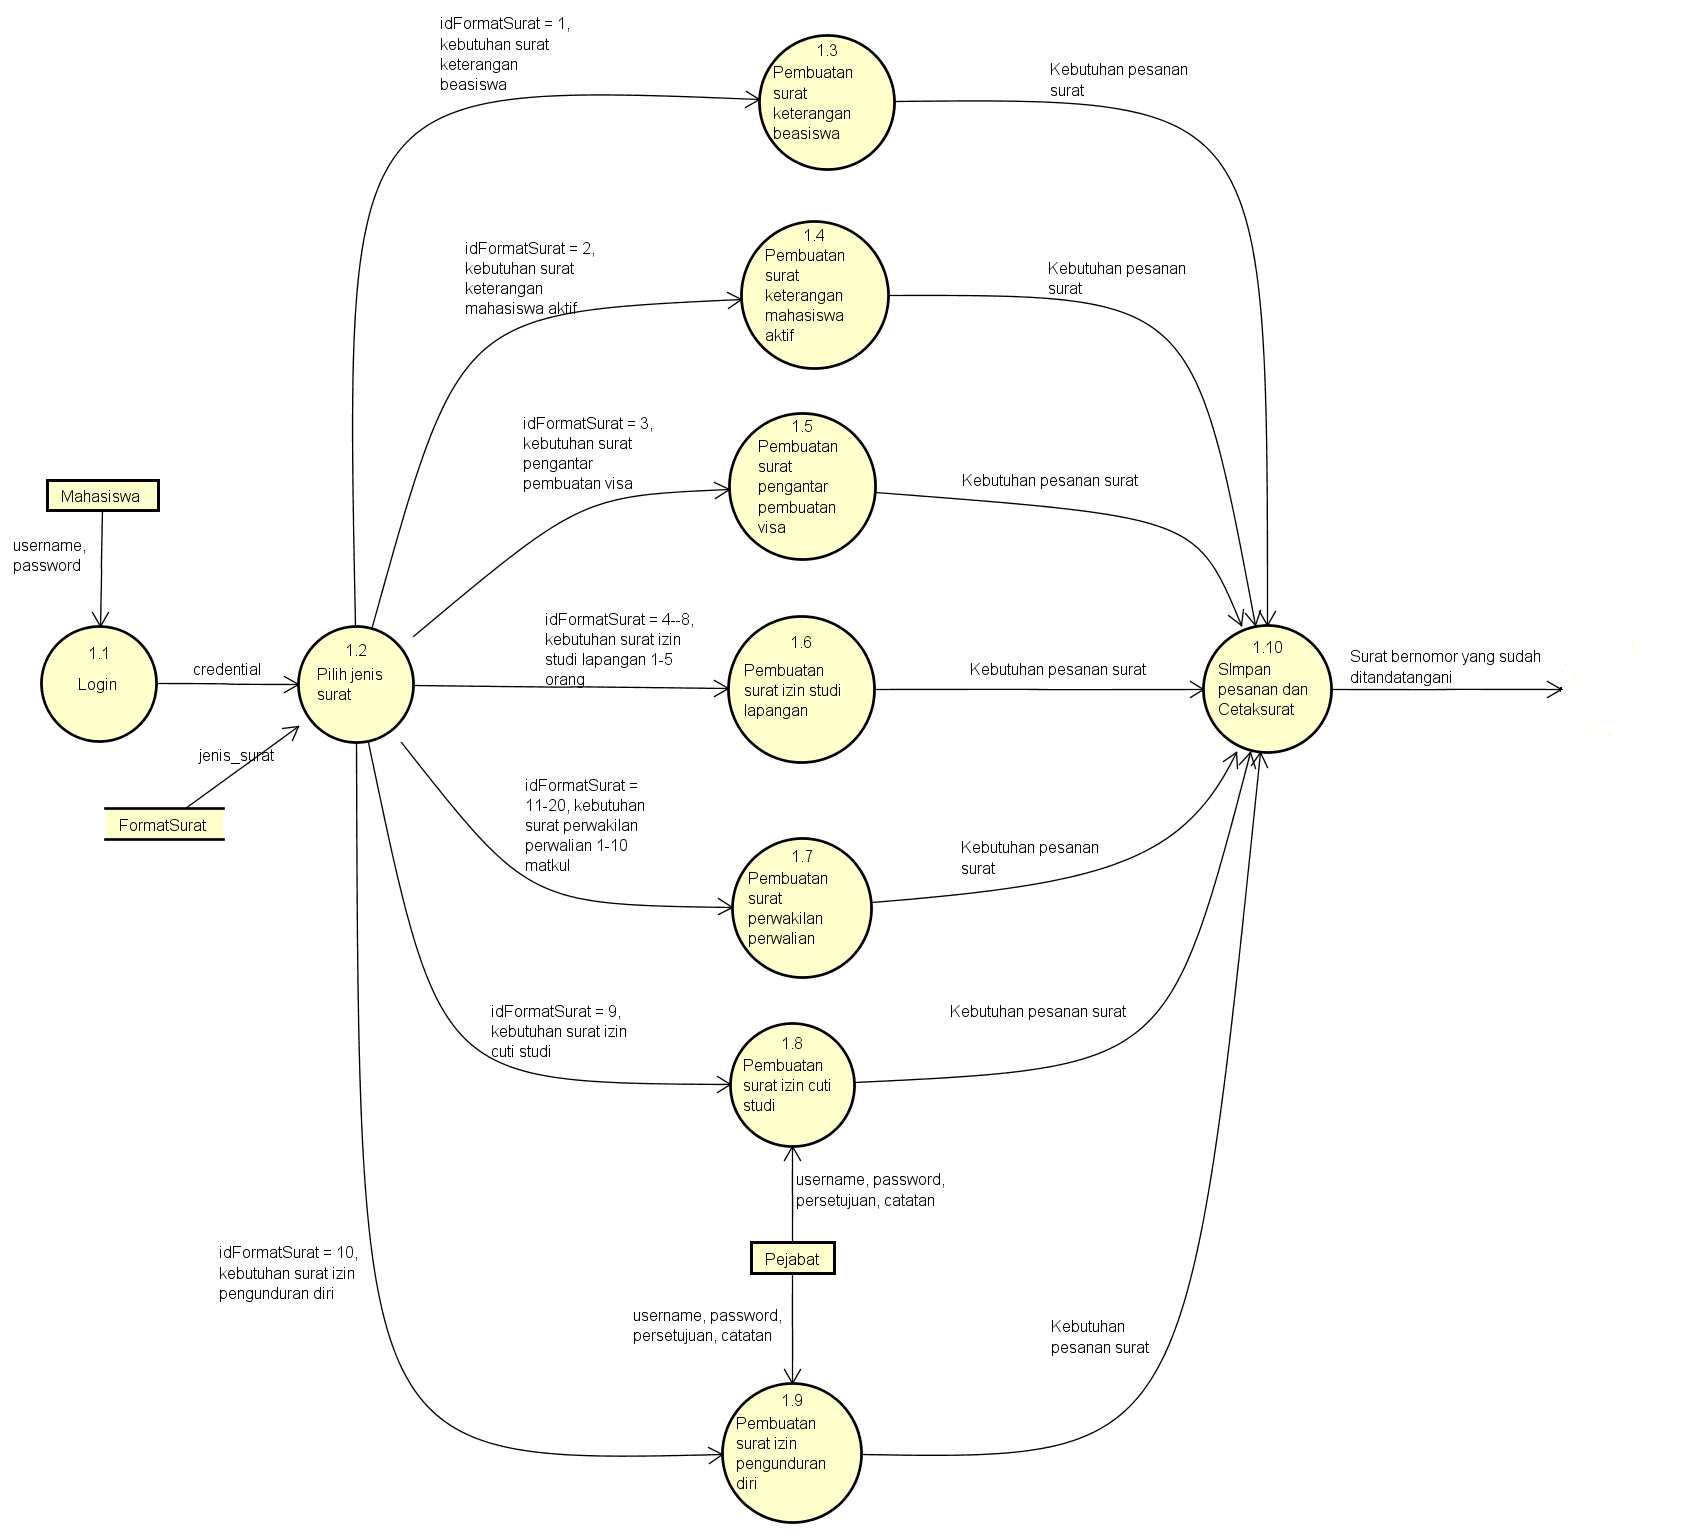
\includegraphics[scale = 0.4]{F:/Skripsi/Dokumentasi_Skripsi/Gambar/Diagram/sistem_usulan/dfd/Lv2-1_buat_suratt.png}
	\caption{DFD \textit{level} 2-1 untuk pembuatan surat}
	\label{fig:level_2-1}
\end{figure}

\begin{figure}[H]
	\centering
		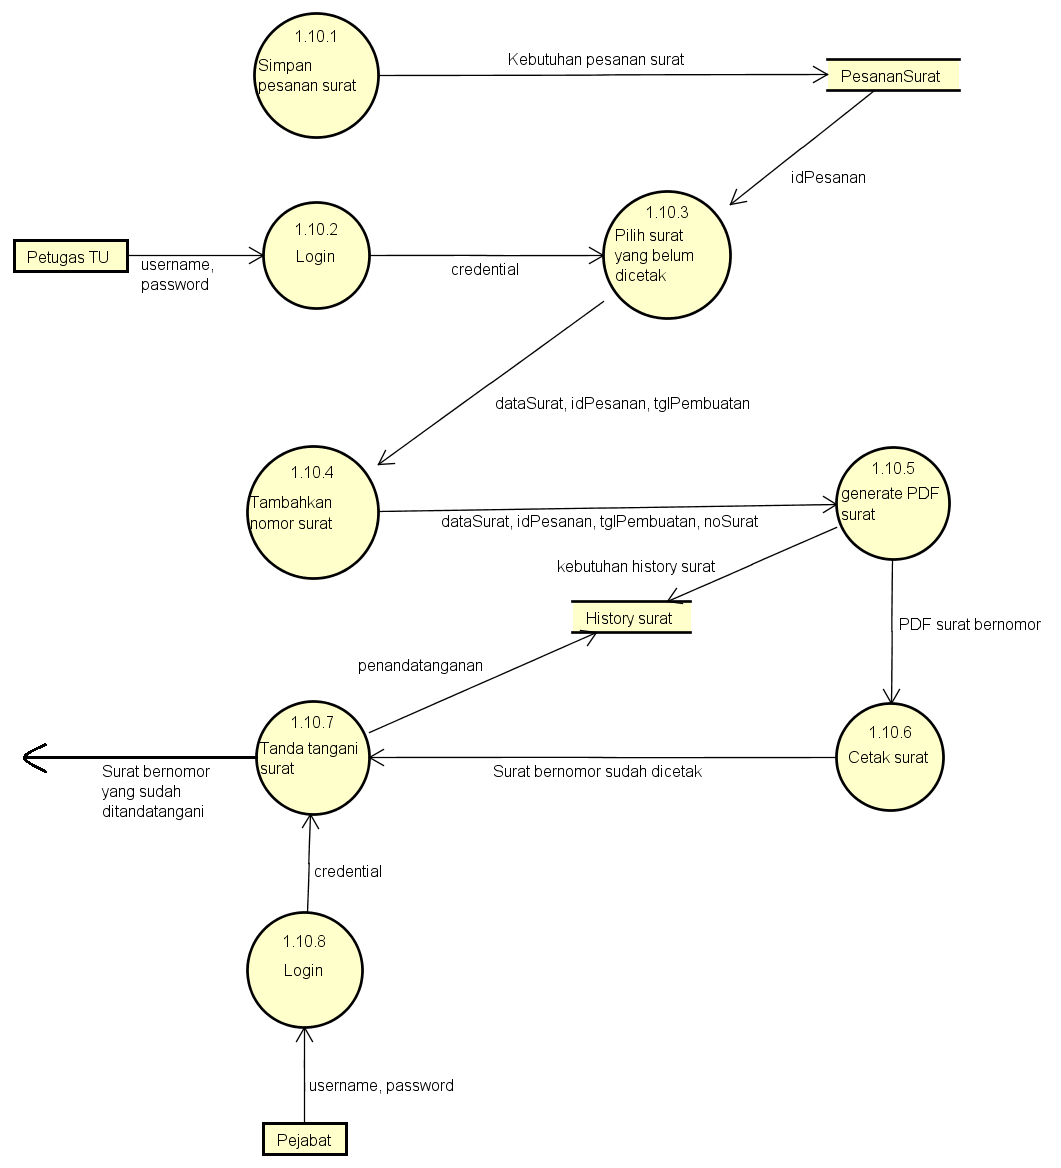
\includegraphics[scale = 0.5]{F:/Skripsi/Dokumentasi_Skripsi/Gambar/Diagram/sistem_usulan/dfd/Lv3-1_10_buat_surat_lanjutan.png}
	\caption{DFD \textit{level} 3-1.10 sebagai lanjutan untuk proses pembuatan surat}
	\label{fig:level_3-1.10}
\end{figure}

Gambar \hyperlink{level_3-1.3}{3.11} merupakan DFD \textit{level} 3-1.3 yang menjelaskan aliran data apabila aktor mahasiswa hendak membuat surat keterangan beasiswa.
\begin{figure}[H]
	\centering
		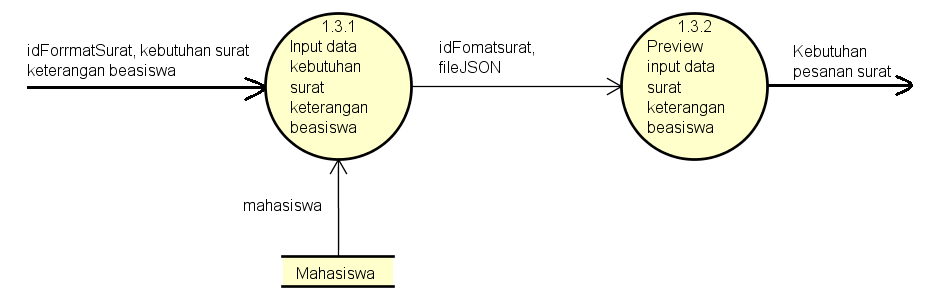
\includegraphics[scale = 0.65]{F:/Skripsi/Dokumentasi_Skripsi/Gambar/Diagram/sistem_usulan/dfd/Lv3-1_3_input_keterangan_beasiswa.png}
	\caption{DFD \textit{level} 3-1.3 untuk pembuatan surat keterangan beasiswa}
	\label{fig:level_3-1.3}
\end{figure}

Gambar \hyperlink{level_3-1.4}{3.12} merupakan DFD \textit{level} 3-1.4 yang menjelaskan aliran data apabila aktor mahasiswa hendak membuat surat keterangan mahasiswa aktif.
\begin{figure}[H]
	\centering
		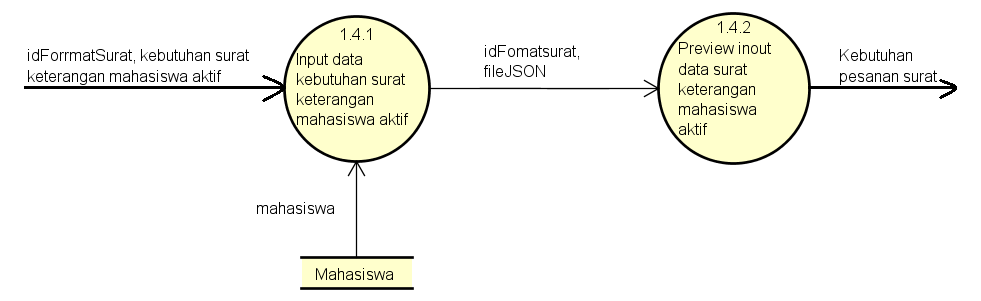
\includegraphics[scale = 0.6]{F:/Skripsi/Dokumentasi_Skripsi/Gambar/Diagram/sistem_usulan/dfd/Lv3-1_4_input_keterangan_mahasiswa_aktif.png}
	\caption{DFD \textit{level} 3-1.4 untuk pembuatan surat keterangan mahasiswa aktif}
	\label{fig:level_3-1.4}
\end{figure}

Gambar \hyperlink{level_3-1.6}{3.13} merupakan DFD \textit{level} 3-1.6 yang menjelaskan aliran data apabila aktor mahasiswa hendak membuat surat pembuatan visa.
\begin{figure}[H]
	\centering
		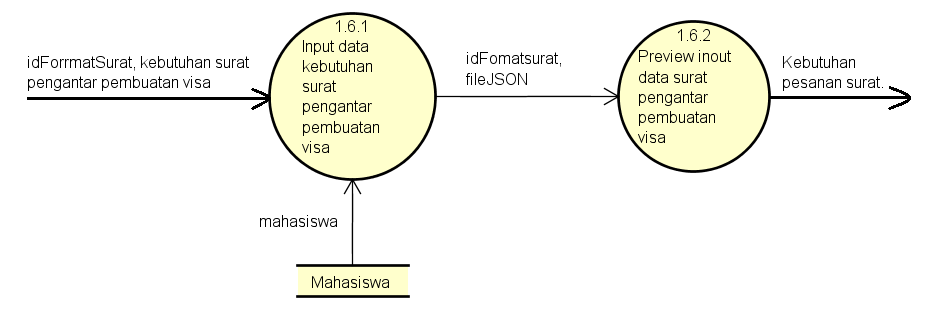
\includegraphics[scale = 0.6]{F:/Skripsi/Dokumentasi_Skripsi/Gambar/Diagram/sistem_usulan/dfd/Lv3-1_6_input_pengantar_pembuatan_visa.png}
	\caption{DFD \textit{level} 3-1.6 untuk pembuatan surat keterangan mahasiswa aktif}
	\label{fig:level_3-1.6}
\end{figure}

Gambar \hyperlink{level_3-1.5}{3.14} merupakan DFD \textit{level} 3-1.5 yang menjelaskan aliran data apabila aktor mahasiswa hendak membuat surat izin studi lapangan.
\begin{figure}[H]
	\centering
		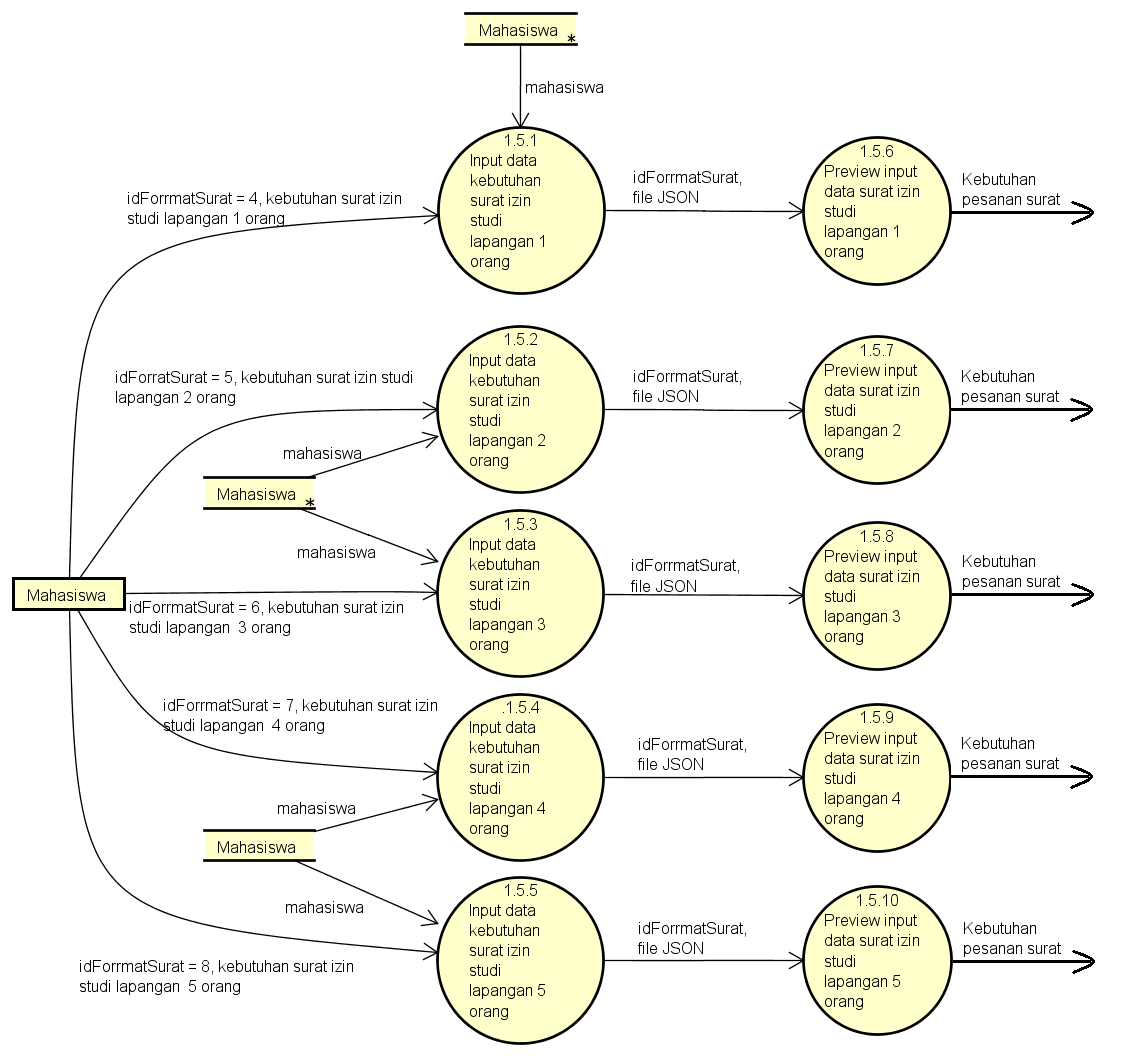
\includegraphics[scale = 0.55]{F:/Skripsi/Dokumentasi_Skripsi/Gambar/Diagram/sistem_usulan/dfd/Lv3-1_5_input_izin_studi_lapangan.png}
	\caption{DFD \textit{level} 3-1.5 untuk pembuatan surat izin studi lapangan}
	\label{fig:level_3-1.5}
\end{figure}

Gambar \hyperlink{level_3-1.7}{3.15} merupakan DFD \textit{level} 3-1.7 yang menjelaskan aliran data apabila aktor mahasiswa hendak membuat surat perwakilan perwalian.
\begin{figure}[H]
	\centering
		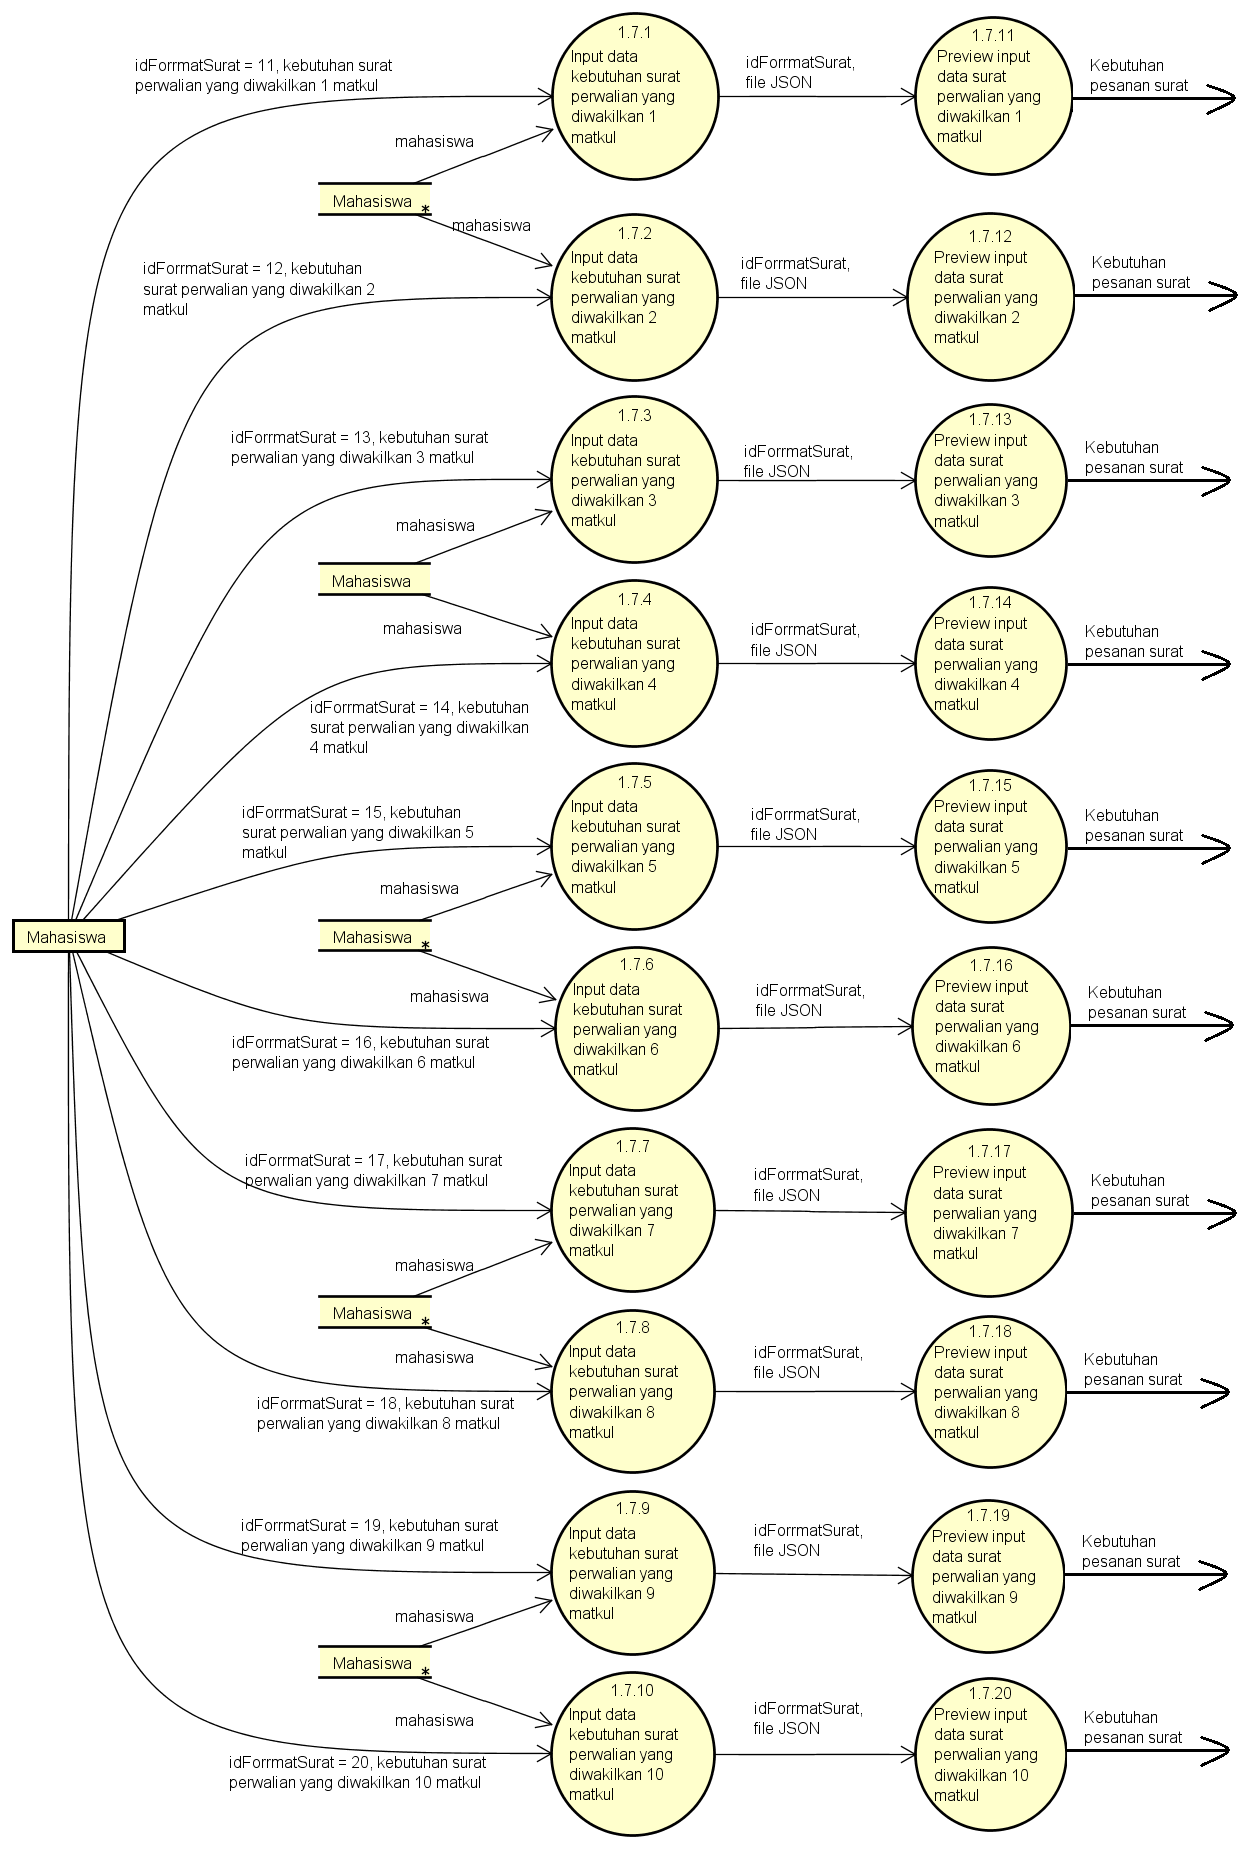
\includegraphics[scale = 0.45]{F:/Skripsi/Dokumentasi_Skripsi/Gambar/Diagram/sistem_usulan/dfd/Lv3-1_7_input_perwakilan_perwalian.png}
	\caption{DFD \textit{level} 3-1.7 untuk pembuatan surat perwakilan perwalian}
	\label{fig:level_3-1.7}
\end{figure}

Gambar \hyperlink{level_3-1.8}{3.16} merupakan DFD \textit{level} 3-1.8 yang menjelaskan aliran data apabila aktor mahasiswa hendak membuat surat izin cuti studi.
\begin{figure}[H]
	\centering
		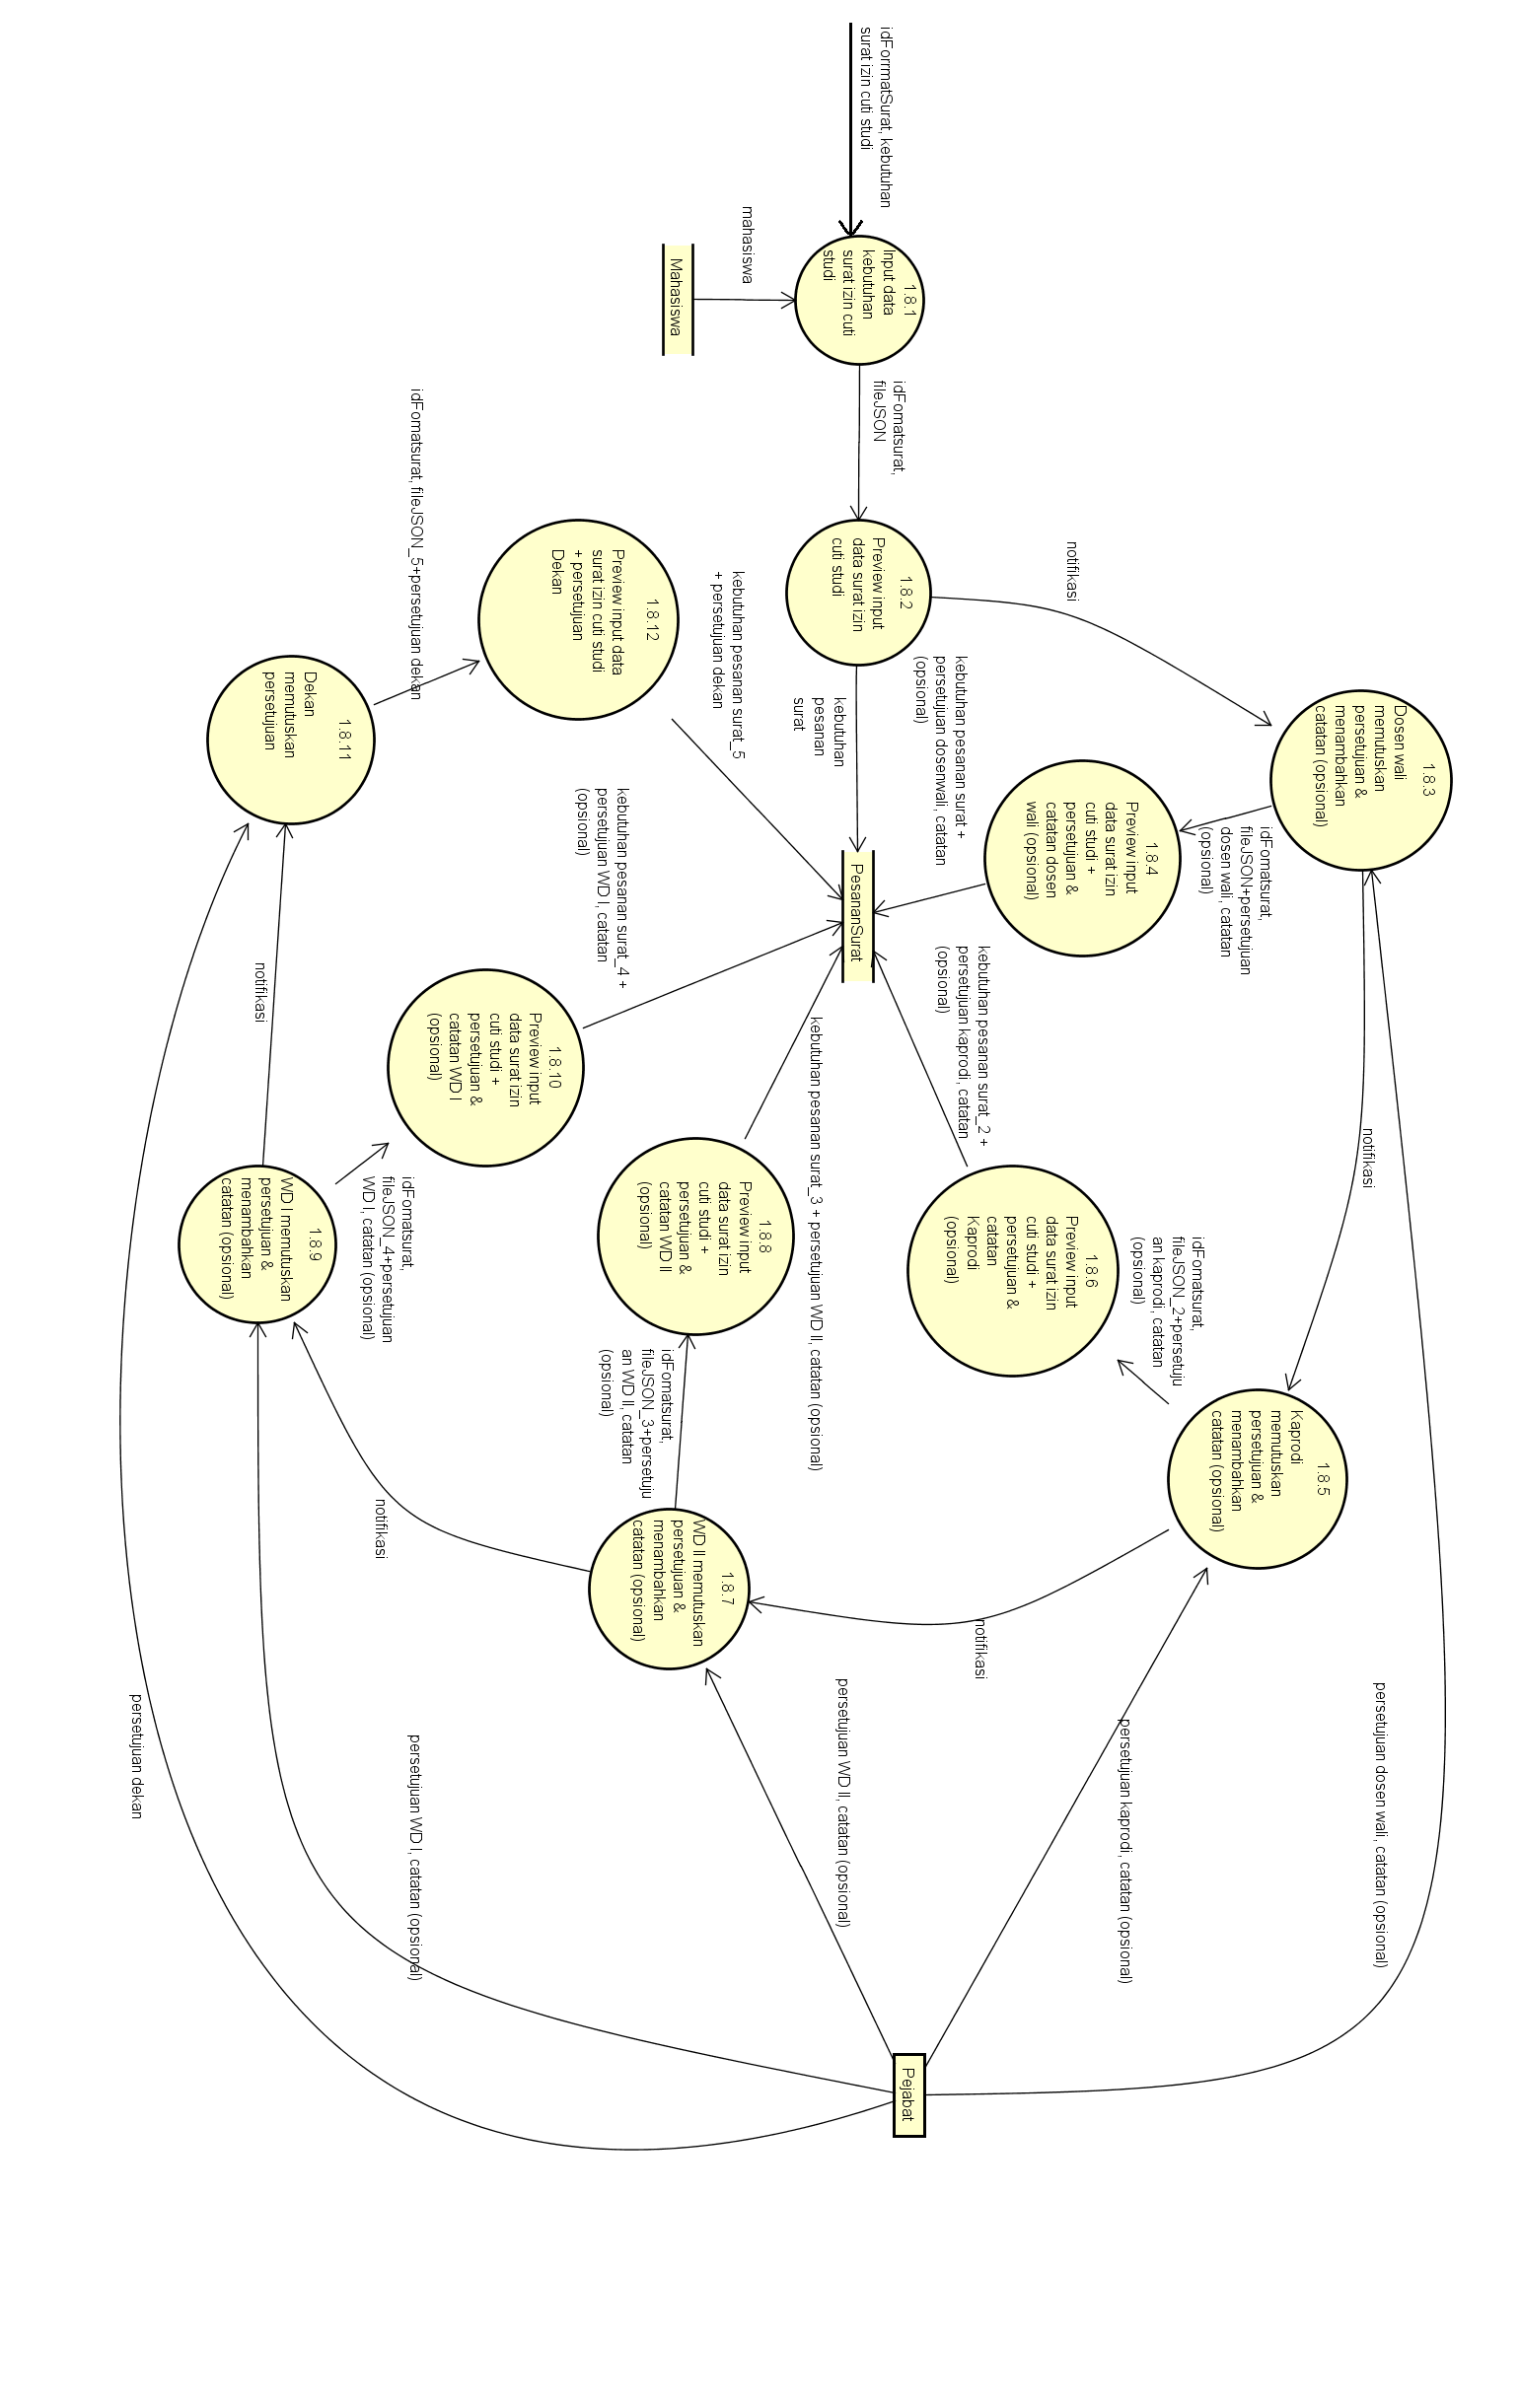
\includegraphics[scale = 0.35]{F:/Skripsi/Dokumentasi_Skripsi/Gambar/Diagram/sistem_usulan/dfd/Lv3-1_8_input_izin_cuti_studi-kiri.png}
	\caption{DFD \textit{level} 3-1.8 untuk pembuatan surat izin cuti studi}
	\label{fig:level_3-1.8}
\end{figure}

Gambar \hyperlink{level_3-1.9}{3.17} merupakan DFD \textit{level} 3-1.9 yang menjelaskan aliran data apabila aktor mahasiswa hendak membuat surat izin pengunduran diri.
\begin{figure}[H]
	\centering
		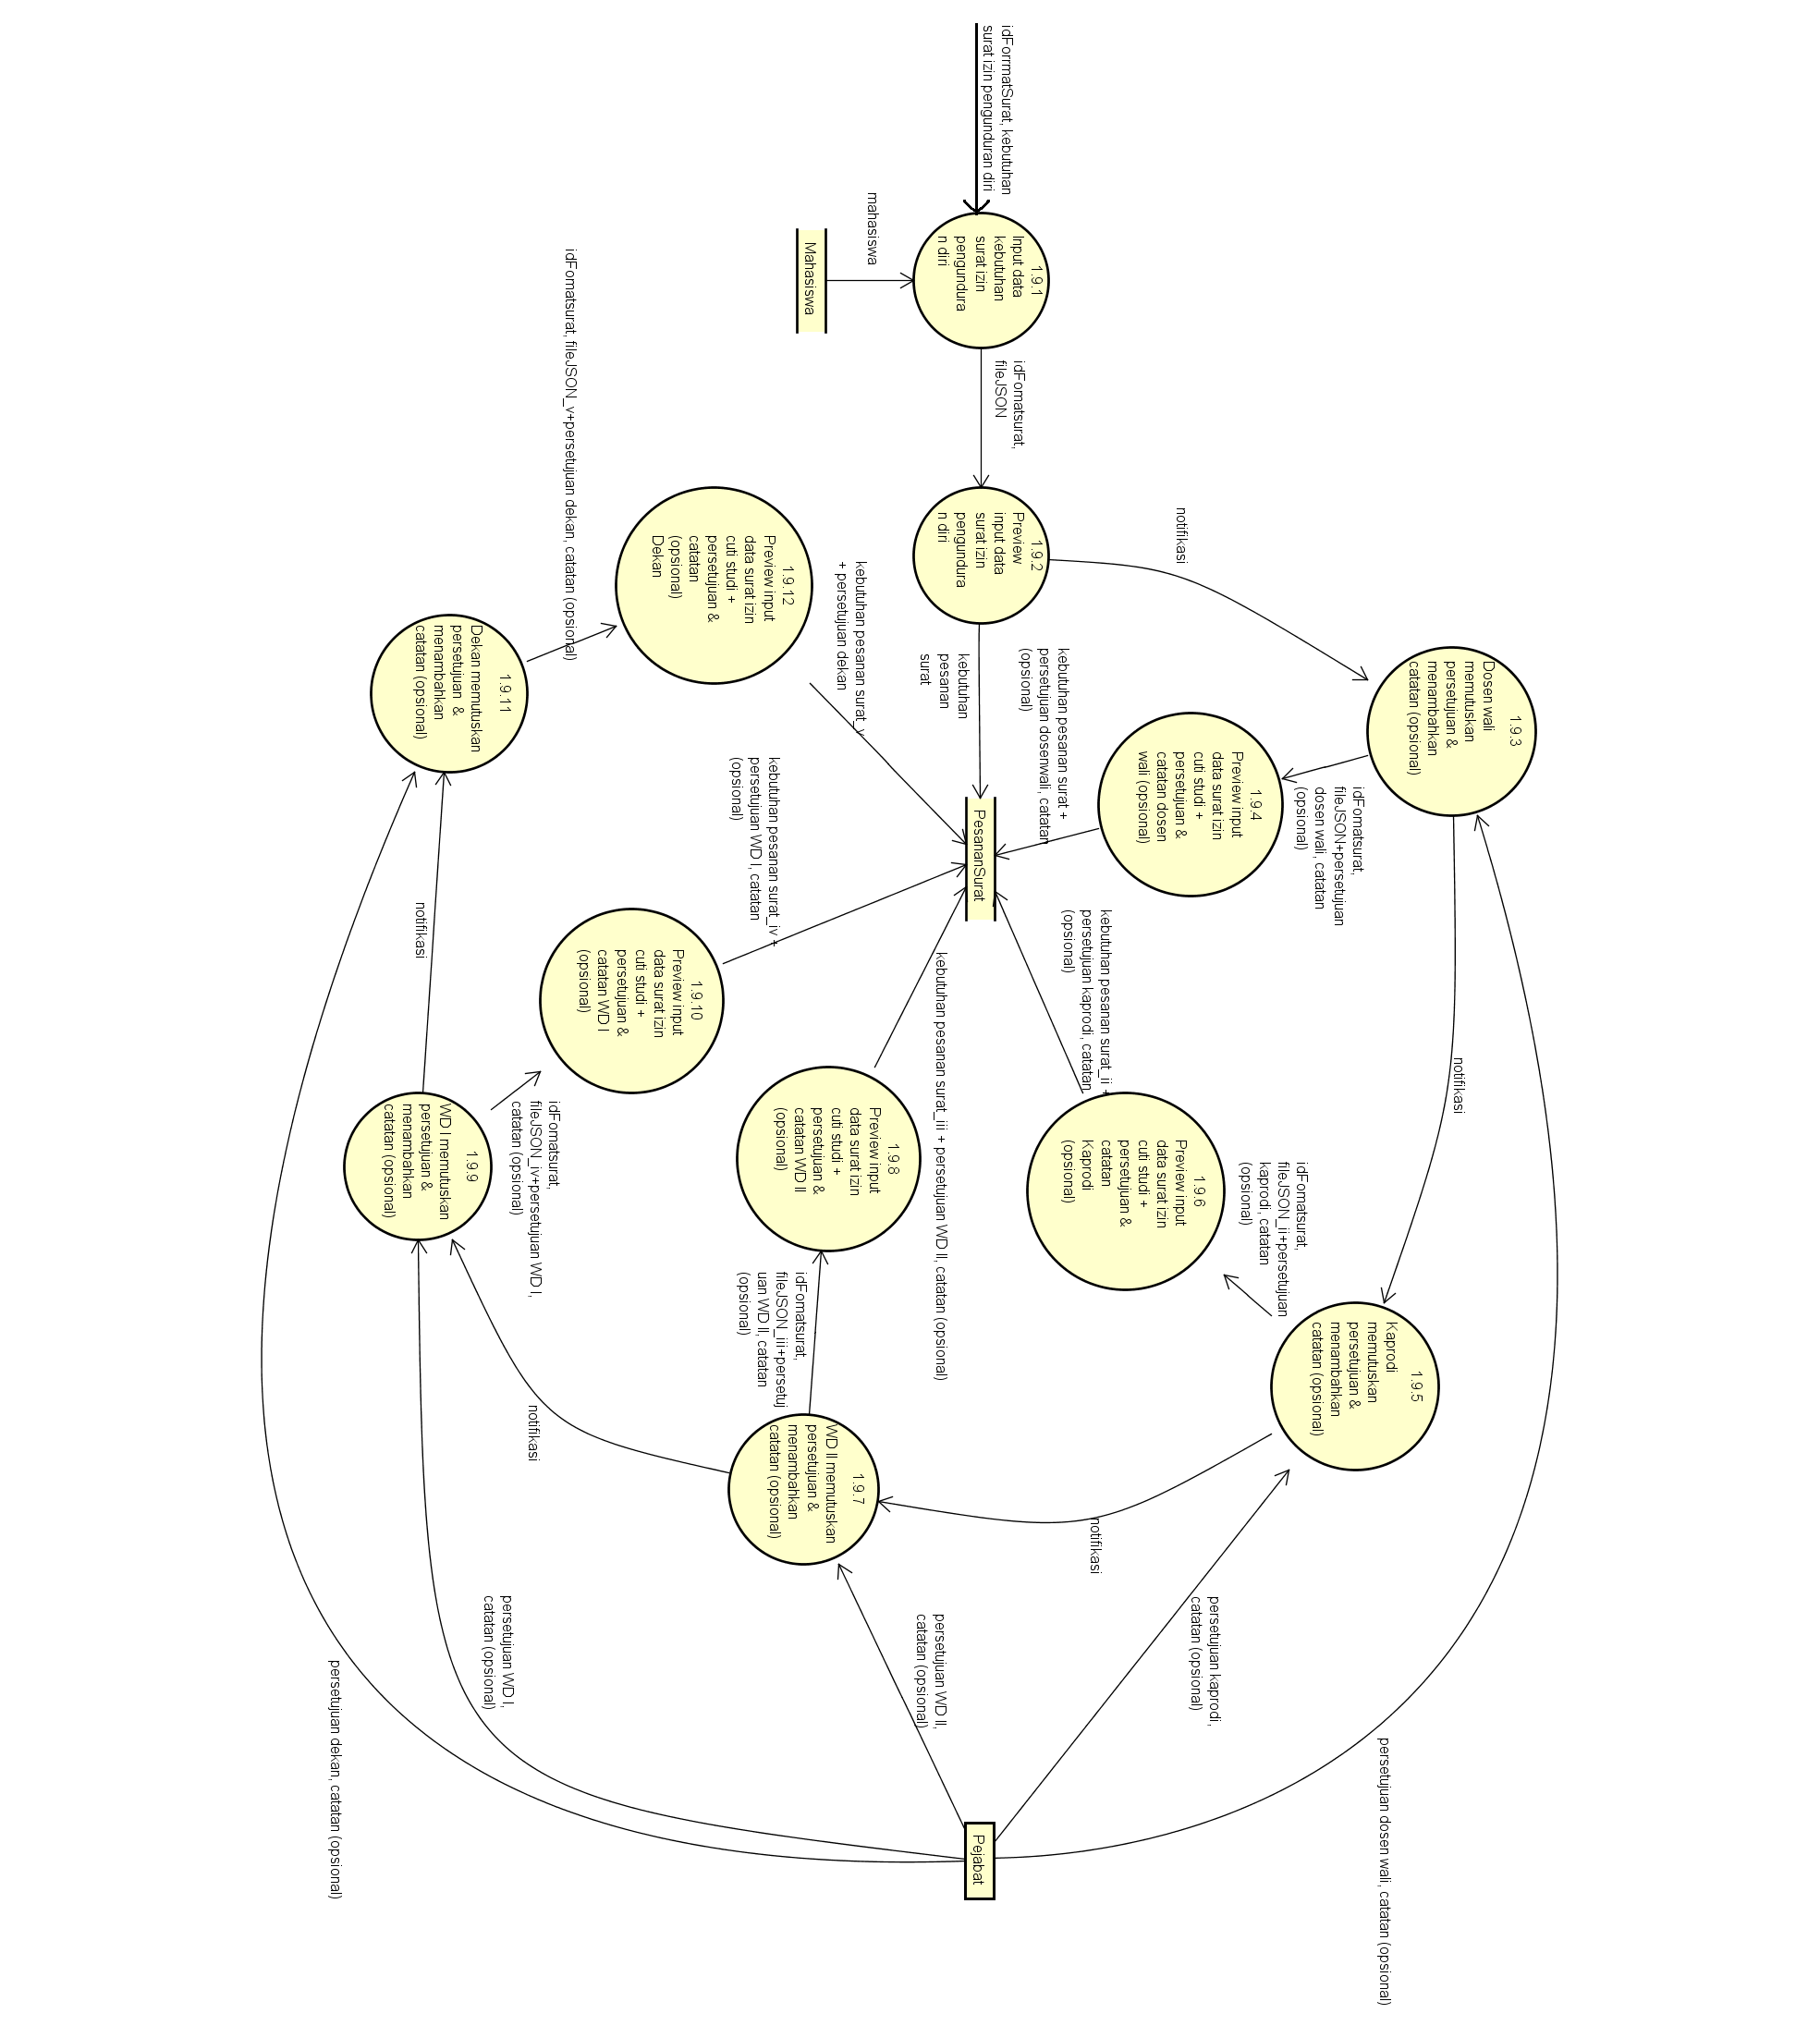
\includegraphics[scale = 0.35]{F:/Skripsi/Dokumentasi_Skripsi/Gambar/Diagram/sistem_usulan/dfd/Lv3-1_9_input_izin_pengunduran_diri-kiri.png}
	\caption{DFD \textit{level} 3-1.9 untuk pembuatan surat izin pengunduran diri}
	\label{fig:level_3-1.9}
\end{figure}

Gambar \hyperlink{level_2-2}{3.18} merupakan DFD \textit{level} 2-2 yang menjelaskan aliran data pada saat aktor mahasiswa hendak mengambil surat.

\begin{figure}[H]
	\centering
		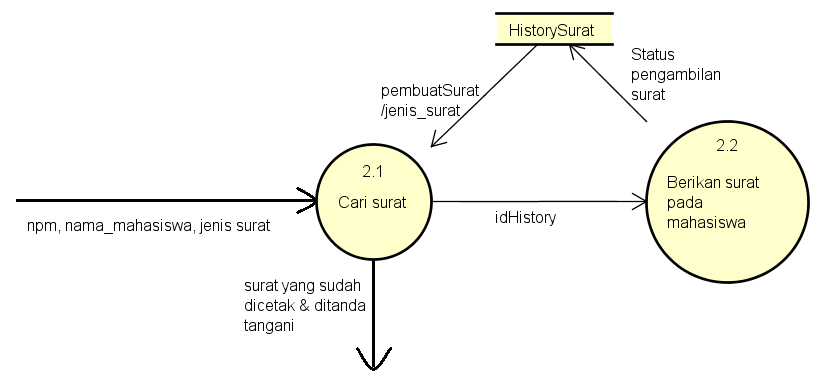
\includegraphics[scale = 0.5]{F:/Skripsi/Dokumentasi_Skripsi/Gambar/Diagram/sistem_usulan/dfd/Lv2-2_pengambilan_surat.png}
	\caption{DFD \textit{level} 2-2 pengambilan surat}
	\label{fig:level_2-2}
\end{figure}

Gambar \hyperlink{level_2-3}{3.19} merupakan DFD \textit{level} 2-3 yang menjelaskan aliran data pada saat aktor petugas TU melakukan operasi CRUD pada \textit{database} format surat.

\begin{figure}[H]
	\centering
		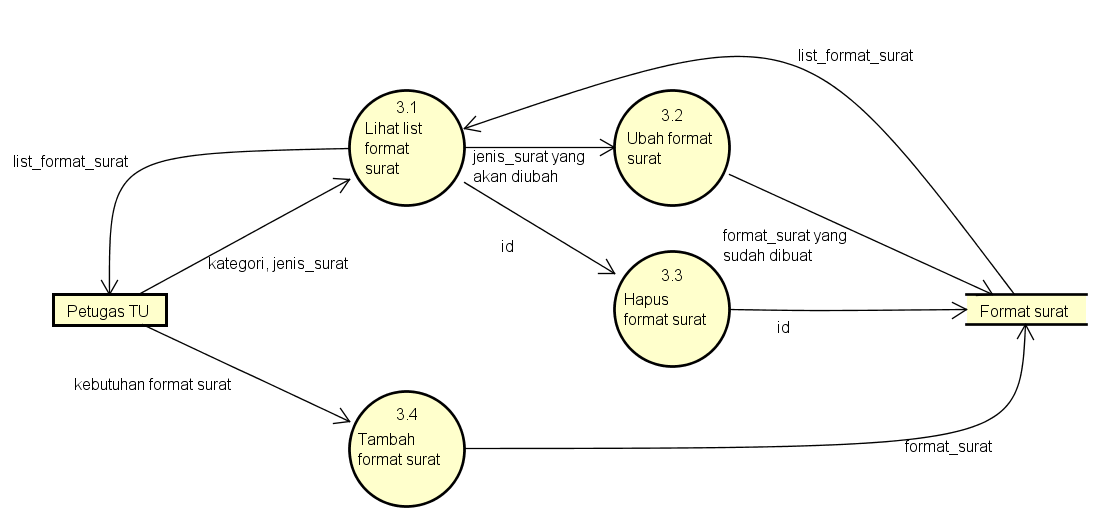
\includegraphics[scale = 0.5]{F:/Skripsi/Dokumentasi_Skripsi/Gambar/Diagram/sistem_usulan/dfd/Lv2-3_kelola_format_surat.png}
	\caption{DFD \textit{level} 2-3 operasi CRUD pada \textit{database} format surat}
	\label{fig:level_2-3}
\end{figure}

Gambar \hyperlink{level_2-4}{3.20} merupakan DFD \textit{level} 2-4 yang menjelaskan aliran data pada saat aktor petugas TU melakukan operasi CRUD pada \textit{database} data mahasiswa.

\begin{figure}[H]
	\centering
		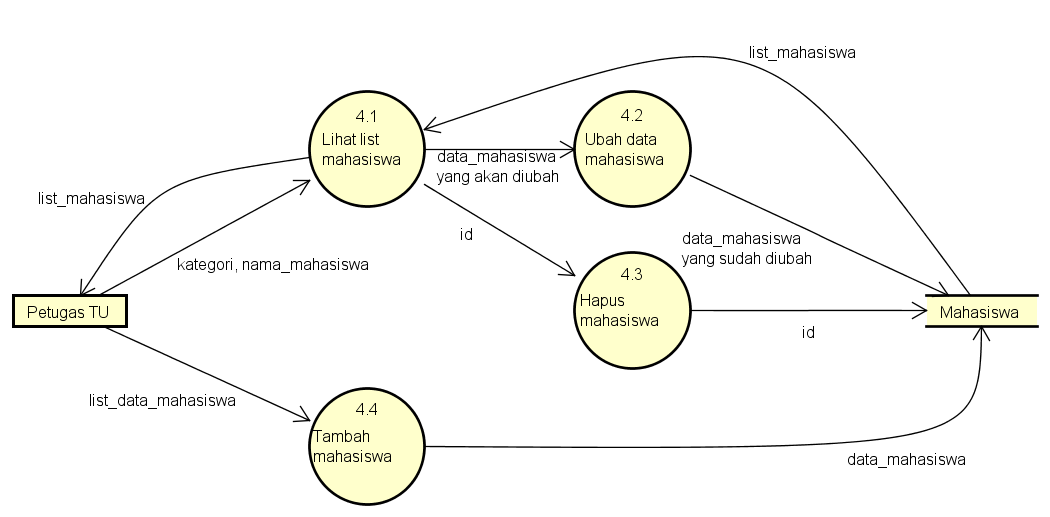
\includegraphics[scale = 0.5]{F:/Skripsi/Dokumentasi_Skripsi/Gambar/Diagram/sistem_usulan/dfd/Lv2-4_kelola_data_mahasiswa.png}
	\caption{DFD \textit{level} 2-4 operasi CRUD pada \textit{database} data mahasiswa}
	\label{fig:level_2-4}
\end{figure}

\textbf{Data Dictionary}\\
\begin{itemize}
 \item list data mahaiswa : nirm, npm, nama mahasiswa, prodi, fakultas, angkatan, tglLahir, kota lahir, foto, dosenWali, username, password
 \item data per mahasiswa : nirm, npm, nama mahasiswa, prodi, fakultas, angkatan, tglLahir, kota lahir, foto, dosenWali
 \item kebutuhan format surat : idFormat, jenis surat, format, keterangan
 \item kebutuhan pesanan surat : tglPembuatan, perihal, npm, idFormatSurat, dataSurat, penerimaSurat
 \item kebutuhan history surat : status penandatanganan surat, Status pengambilan surat
\end{itemize}

\subsection{Analisis Kebutuhan Data}
\label{sec:analisis_kebutuhan_data}
Setiap surat memiliki kebutuhan data yang berbeda-beda bergantung dari jenis surat yang akan dibuat. Tabel 3.16-3.20 berikut ini akan menjelaskan data apa saja yang perlu diisikan oleh mahasiswa dalam proses pembuatan surat akademik.\

\begin{table}[h]
\centering
\caption{Tabel kebutuhan data surat keterangan beasiswa}
\label{surat_keterangan_beasiswa}
\begin{tabular}{|l|}
\hline
\textbf{Atribut Data}                     \\ \hline
Nama mahasiswa                            \\ \hline 
Program studi                             \\ \hline 
NPM                             			\\ \hline
Semester			                        \\ \hline
Tahun akademik        			        \\ \hline
Penyedia beasiswa                         \\ \hline
\end{tabular}
\end{table}

\begin{table}[h]
\centering
\caption{Tabel kebutuhan data surat keterangan mahasiswa aktif}
\label{surat_keterangan_mahasiswa_aktif}
\begin{tabular}{|l|}
\hline
\textbf{Atribut Data}                     \\ \hline
Nama mahasiswa                            \\ \hline 
Program studi                             \\ \hline 
NPM                             			\\ \hline 
Semester                     				\\ \hline 
Tahun akademik                         	\\ \hline 
Kota lahir               					\\ \hline 
Tanggal lahir             				\\ \hline 
Alamat di Bandung                    		\\ \hline 
\end{tabular}
\end{table}

\begin{table}[h]
\centering
\caption{Tabel kebutuhan data surat pengantar pembuatan visa}
\label{surat_pengantar_pembuatan_visa}
\begin{tabular}{|l|}
\hline
\textbf{Atribut Data}                     \\ \hline
Nama mahasiswa                            \\ \hline 
Tanggal lahir                    			\\ \hline 
Kewarganegaraan                     	    \\ \hline 
Tahun akademik              				\\ \hline 
Organisasi tujuan         			    \\ \hline 
Negara tujuan              			    \\ \hline 
Tanggal kunjungan                         \\ \hline 
\end{tabular}
\end{table}

\begin{table}[h]
\centering
\caption{Tabel kebutuhan data surat pengantar studi lapangan}
\label{surat_keterangan_beasiswa}
\begin{tabular}{|l|}
\hline
\textbf{Atribut Data}                     \\ \hline
Nama mahasiswa                            \\ \hline 
NPM                                      \\ \hline 
Program studi                             \\ \hline
Mata kuliah			                    \\ \hline
Topik        			                    \\ \hline
Organisasi tujuan                         \\ \hline
Alamat organisasi tujuan                  \\ \hline
Keperluan kunjungan                       \\ \hline
Data rekan(nama, NPM rekan)(opsional)     \\ \hline

\end{tabular}
\end{table}

\begin{table}[H]
\centering
\caption{Tabel kebutuhan data surat izin cuti studi}
\label{surat_izin_cuti_studi}
\begin{tabular}{|l|}
\hline
{\textbf{Atribut Data}}                     \\ \hline
Nama mahasiswa                            \\ \hline 
NPM                                       \\ \hline 
Fakultas                                  \\ \hline 
Program studi                             \\ \hline 
Alamat tetap                              \\ \hline
Cuti studi ke-n   			            \\ \hline 
Alasan cuti studi ke-n                    \\ \hline
Dosen Wali				                \\ \hline 
Catatan Dosen Wali                        \\ \hline
Catatan Ketua Progam Studi                \\ \hline 
Rekomendasi Pembantu Dekan II             \\ \hline 
Rekomendasi Pembantu Dekan I              \\ \hline 
Semester                          		\\ \hline 
Tahun akademik                            \\ \hline
Persetujuan Dekan                         \\ \hline 
Tanggal surat                             \\ \hline
\end{tabular}
\end{table}

\begin{table}[H]
\centering
\caption{Tabel kebutuhan data surat izin pengunduran diri}
\label{surat_izin_pengunduran_diri}
\begin{tabular}{|l|}
\hline
\textbf{Atribut Data}                     \\ \hline
Nama mahasiswa                            \\ \hline 
NPM                                       \\ \hline 
NIRM                                      \\ \hline 
Alamat (tetap/di Badung)                  \\ \hline 
Nomor telepon (HP)                        \\ \hline 
Nama orang tua                            \\ \hline 
Tanggal surat                             \\ \hline 
Semester berhenti                         \\ \hline 
Catatan Dosen Wali                        \\ \hline 
Catatan Ketua Program Studi               \\ \hline 
Catatan Wakil Dekan I                     \\ \hline 
Catatan Wakil Dekan II                    \\ \hline 
Catatan Dekan                             \\ \hline
\end{tabular}
\end{table}

\begin{table}[H]
\centering
\caption{Tabel kebutuhan data surat perwakilan perwalian}
\label{surat_perwakilan_perwalian}
\begin{tabular}{|l|}
\hline
\textbf{Atribut Data}                      \\ \hline
Semester            					   \\ \hline
Tahun akademik							   \\ \hline
Nama mahasiswa yang diwakilkan             \\ \hline 
NPM mahasiswa yang diwakilkan              \\ \hline 
Program Studi mahasiswa yang diwakilkan    \\ \hline 
Nama mahasiswa yang diberi kuasa           \\ \hline 
NPM mahasiswa yang diberi kuasa            \\ \hline 
Program studi mahasiswa yang diberi kuasa  \\ \hline 
Alasan tidak hadir perwalian               \\ \hline 
Mata kuliah yang diambil (maks. 10 mata kuliah)                  \\ \hline 
Tanggal pembuatan surat                    \\ \hline
Nama dosen wali							   \\ \hline
Nama wakil dekan I						   \\ \hline
\end{tabular}
\end{table}

\subsection{ER Diagram}
\label{sec:er_diagram}
Setelah mengamati \textit{work flowmap}, didapat beberapa objek yang dapat digambarkan menjadi sebuah entitas pada diagram ER. Objek-objek yang dimaksud yaitu format surat, mahasiswa, petugas TU dan pejabat. Untuk objek surat dan mahasiswa dapat langsung dibuat entitas. Untuk objek pejabat diubah menjadi entitas dosen karena pejabat merupakan dosen yang memiliki pangkat tertentu di jurusan maupun fakultas.\

Selain objek yang didapat dari \textit{work flowmap}, didapat juga objek-objek lain yang berhubungan dengan objek-objek yang telah disebutkan. Objek-objek yang dimaksud yaitu jurusan, fakultas, pesanan surat dan \textit{history} surat. Gambar \hyperlink{erd}{3.21} adalah diagram ER yang menggambarkan hubungan antar entitas yang telah disebutkan di atas.

\begin{figure}[H]
	\centering
		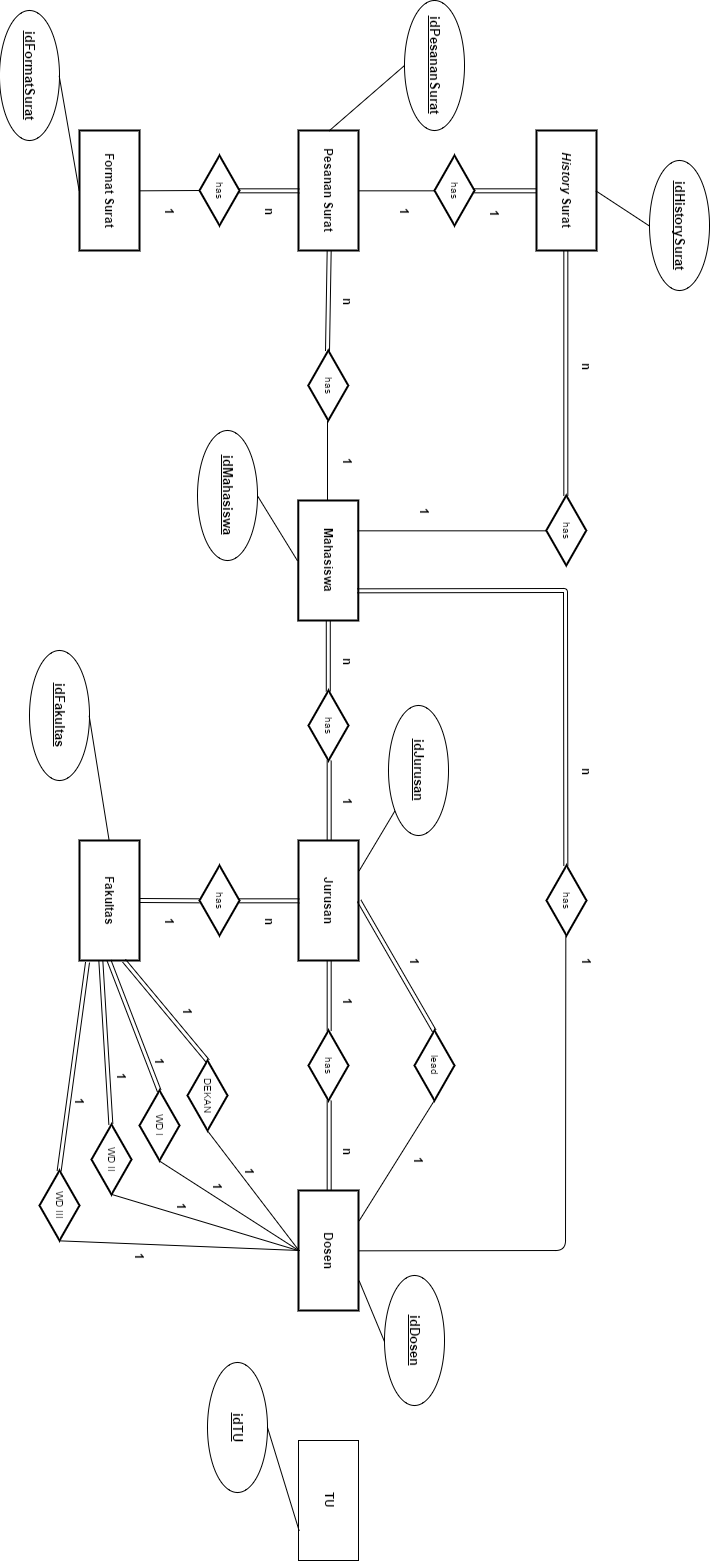
\includegraphics[scale = 0.5]{F:/Skripsi/Dokumentasi_Skripsi/Gambar/Diagram/sistem_usulan/erd/erd_left.png}
	\caption{Diagram ER}
	\label{fig:level_2-2}
\end{figure}}{}
\ifdefstring{\vbabd}{1}{\chapter{Perancangan}
\label{chap:perancangan}
Bab ini membahas mengenai perancangan struktur modul, perancangan basis data dan perancangan antar muka.

\section{Perancangan Struktur Modul}
\label{sec:perancangan_struktur_modul}
Berdasarkan \textit{work-flowmap} yang telah dirancang pada bab 3, maka dirancang struktur modul yang menjelaskan mengenai modul-modul apa saja yang akan dirancang untuk membangun \textit{website} SIKSA. Garis besar dari struktur modul ini terbagi menjadi 3 bagian berdasarkan penggunanya, yaitu modul mahasiswa, modul TU dan modul pejabat.\
Gambar \hyperlink{struktur_modul_garis_besar}{4.1} menjelaskan struktur modul secara garis besar.

\begin{figure}[H]
	\centering
		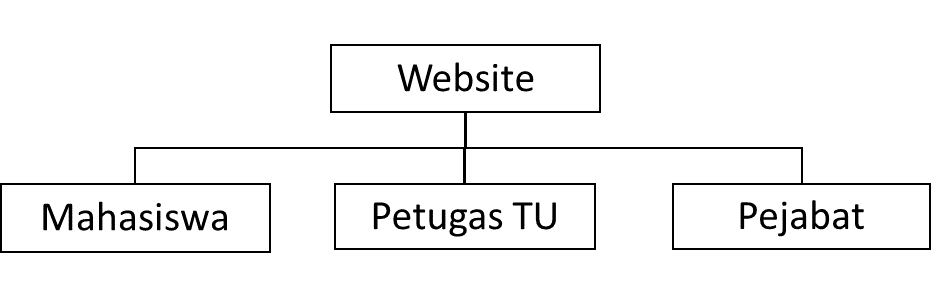
\includegraphics[scale=0.65]{F:/Skripsi/Dokumentasi_Skripsi/Gambar/Struktur_Modul/modul_utama.png}
	\caption{Struktur modul secara garis besar}
	\label{fig:struktur_modul_garis_besar}
\end{figure}

Selanjutnya, modul-modul yang telah disebutkan sebelumnya memiliki struktur tersendiri yang lebih spesifik. Gambar \hyperlink{struktur_modul_mahasiswa}{4.2} menjelaskan struktur modul mahasiswa secara menyeluruh.

\begin{figure}[H]
	\centering
		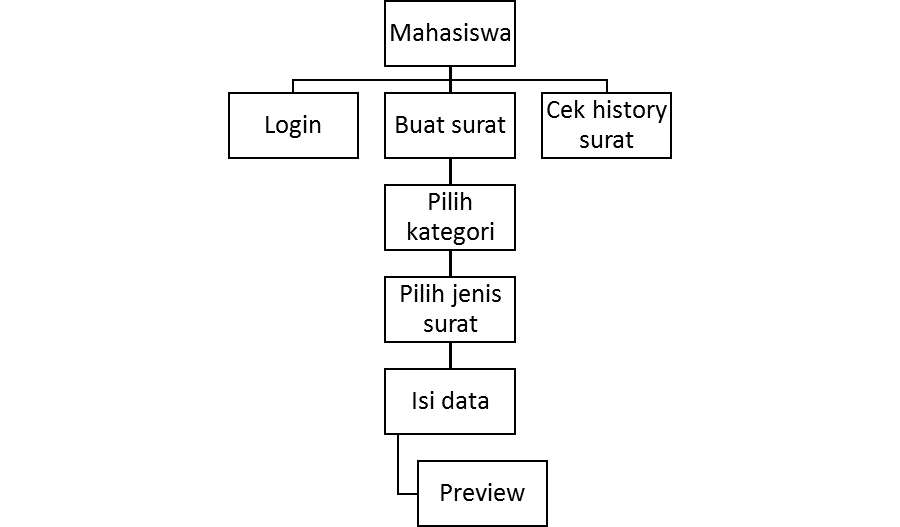
\includegraphics[scale=0.85]{F:/Skripsi/Dokumentasi_Skripsi/Gambar/Struktur_Modul/modul_mahasiswa.png}
	\caption{Struktur modul mahasiswa}
	\label{fig:struktur_modul_mahasiswa}
\end{figure}

Berdasarkan gambar di atas, berikut ini adalah penjelasan mengenai struktur modul mahasiswa dari \textit{website} SIKSA :
\begin{enumerate}
	\item Modul \textit{login}.
	\item Modul untuk membuat surat.
	\item Modul untuk mengecek \textit{history} pembuatan surat.
\end{enumerate}

Gambar \hyperlink{struktur_modul_tu}{4.3} menjelaskan struktur modul petugas TU secara menyeluruh.

\begin{figure}[H]
	\centering
		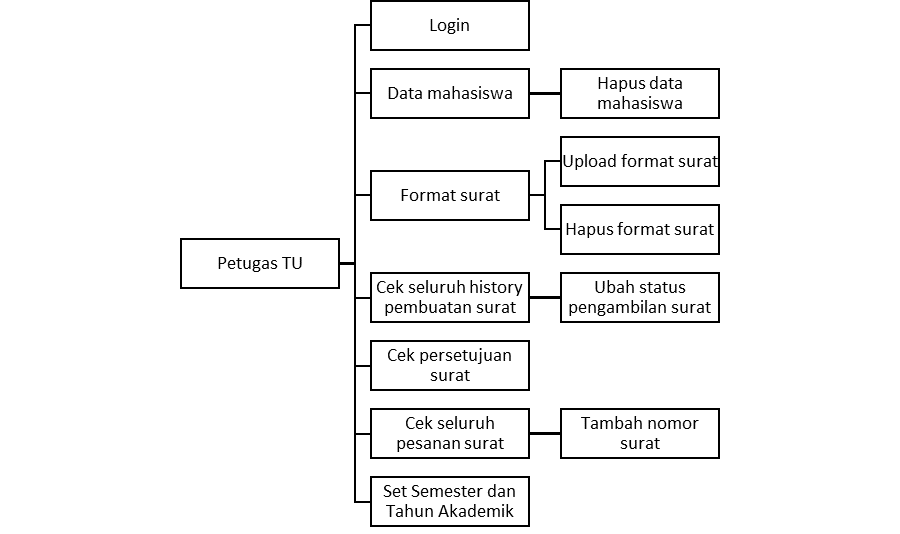
\includegraphics[scale=0.95]{F:/Skripsi/Dokumentasi_Skripsi/Gambar/Struktur_Modul/modul_TU-rev.png}
	\caption{Struktur modul petugas TU}
	\label{fig:struktur_modul_TU}
\end{figure}

Berdasarkan gambar di atas, berikut ini adalah penjelasan mengenai struktur modul TU dari \textit{website} SIKSA :
\begin{enumerate}
	\item Modul \textit{login}.
	\item Modul untuk melihat data mahasiswa.
	\item Modul untuk melihat format surat.
	\item Modul untuk mengecek seluruh \textit{history} pembuatan surat.
	\item Modul untuk mengecek seluruh pesanan surat yang masuk.
	\item Modul untuk mengubah semester dan tahun akademik terkini.
\end{enumerate}

Gambar \hyperlink{struktur_modul_pejabat}{4.4} menjelaskan struktur modul pejabat secara menyeluruh.

\begin{figure}[H]
	\centering
		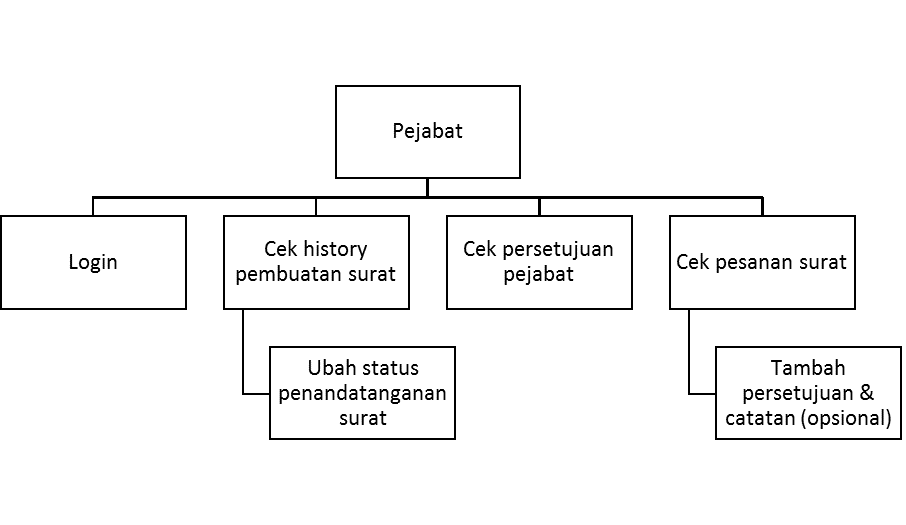
\includegraphics[scale=0.75]{F:/Skripsi/Dokumentasi_Skripsi/Gambar/Struktur_Modul/modul_pejabat.png}
	\caption{Struktur modul pejabat}
	\label{fig:struktur_modul_pejabat}
\end{figure}

Berdasarkan gambar di atas, berikut ini adalah penjelasan mengenai struktur modul pejabat dari \textit{website} SIKSA :
\begin{enumerate}
	\item Modul \textit{login}.
	\item Modul untuk mengecek \textit{history} pembuatan surat.
	\item Modul untuk mengecek pesanan surat yang masuk.
\end{enumerate}

\section{Perancangan Fisik Basis Data}
\label{sec:perancangan_fisik_basis_data}
Berdasarkan diagram ER yang telah dibuat pada bab 3, dapat dibangun perancangan fisik dari basis data untuk mengimplementasikan hubungan antar entitas.\

Tabel \ref{entitas_mahasiswa}-\ref{entitas_petugas_TU} berikut ini menjelaskan entitas apa saja yang dibangun beserta dengan atribut-atribut pada entitas tersebut.

\begin{table}[H]
\centering
\caption{Tabel entitas mahasiswa}
\label{entitas_mahasiswa}
\begin{tabular}{|l|l|l|l|l|l|}
\hline
\textbf{Nama Field}&\textbf{Tipe Data}&\textbf{Panjang}&\textbf{Ket.}&\textbf{Null?}&\textbf{FK ke Relasi Lain}\\ \hline
Id&int&10&PK&Not null&\\ \hline
NIRM&varchar&255&&Not null&\\ \hline
NPM&varchar&255&&Not null&\\ \hline
Nama&varchar&255&&Not null&\\ \hline
Jurusan&int&11&FK&Not null&Jurusan\\ \hline
Fakultas&int&11&FK&Not null&Fakultas\\ \hline
Angkatan&int&11&&Not null&\\ \hline
Kota lahir&varchar&255&&Not null&\\ \hline
Tanggal lahir&date&&&Not null&\\ \hline
Foto&varchar&255&&Not null&\\ \hline
Dosen wali&int&11&FK&Not null&Dosen\\ \hline
Username&varchar&255&&Not null&\\ \hline
Kewarganegaraan&varchar&255&&Not null&\\ \hline
Semester&varchar&6&&Not null&\\ \hline
Tahun Akademik&varchar&9&&Not null&\\ \hline
\end{tabular}
\end{table}

\begin{table}[H]
\centering
\caption{Tabel entitas dosen}
\label{entitas_dosen}
\begin{tabular}{|l|l|l|l|l|l|}
\hline
\textbf{Nama Field}&\textbf{Tipe Data}&\textbf{Panjang}&\textbf{Ket.}&\textbf{Null?}&\textbf{FK ke Relasi Lain}\\ \hline
Id&int&10&PK&Not null&\\ \hline
NIK&varchar&255&&Not null&\\ \hline
Nama&varchar&255&&Not null&\\ \hline
Jurusan&int&11&FK&Not null&Jurusan\\ \hline
Fakultas&int&11&FK&Not null&Fakultas\\ \hline
Foto&varchar&255&&Not null&\\ \hline
Username&varchar&255&&Not null&\\ \hline
\end{tabular}
\end{table}

\begin{table}[H]
\centering
\caption{Tabel entitas jurusan}
\label{entitas_jurusan}
\begin{tabular}{|l|l|l|l|l|l|}
\hline
\textbf{Nama Field}&\textbf{Tipe Data}&\textbf{Panjang}&\textbf{Ket.}&\textbf{Null?}&\textbf{FK ke Relasi Lain}\\ \hline
Id&int&10&PK&Not null&\\ \hline
Kode jurusan&varchar&255&&Not null&\\ \hline
Nama&varchar&255&&Not null&\\ \hline
Ketua jurusan&int&11&FK&Not null&Dosen\\ \hline
\end{tabular}
\end{table}

\begin{table}[H]
\centering
\caption{Tabel entitas fakultas}
\label{entitas_fakultas}
\begin{tabular}{|l|l|l|l|l|l|}
\hline
\textbf{Nama Field}&\textbf{Tipe Data}&\textbf{Panjang}&\textbf{Ket.}&\textbf{Null?}&\textbf{FK ke Relasi Lain}\\ \hline
Id&int&10&PK&Not null&\\ \hline
Kode fakultas&varchar&255&&Not null&\\ \hline
Nama&varchar&255&&Not null&\\ \hline
Dekan&int&11&PK&Not null&Dosen\\ \hline
Wakil Dekan I&int&11&FK&Not null&Dosen\\ \hline
Wakil Dekan II&int&11&FK&Not null&Dosen\\ \hline
Wakil Dekan III&int&11&FK&Not null&Dosen\\ \hline\end{tabular}
\end{table}

\begin{table}[H]
\centering
\caption{Tabel entitas format surat}
\label{entitas_format_surat}
\begin{tabular}{|l|l|l|l|l|l|}
\hline
\textbf{Nama Field}&\textbf{Tipe Data}&\textbf{Panjang}&\textbf{Ket.}&\textbf{Null?}&\textbf{FK ke Relasi Lain}\\ \hline
Id&int&10&PK&Not null&\\ \hline
Id format&varchar&255&&Not null&\\ \hline
Jenis surat&varchar&255&&Not null&\\ \hline
Keterangan&varchar&255&&Not null&\\ \hline
Link format&varchar&255&&Not null&\\ \hline
\end{tabular}
\end{table}

\begin{table}[H]
\centering
\caption{Tabel entitas pesanan surat}
\label{entitas_pesanan_surat}
\begin{tabular}{|l|l|l|l|l|l|}
\hline
\textbf{Nama Field}&\textbf{Tipe Data}&\textbf{Panjang}&\textbf{Ket.}&\textbf{Null?}&\textbf{FK ke Relasi Lain}\\ \hline
Id&int&10&PK&Not null&\\ \hline
Tanggal buat&timestamp&&&Not null&\\ \hline
Pemohon&int&11&FK&Not null&Mahasiswa\\ \hline
Jenis surat&int&11&FK&Not null&Format surat\\ \hline
Data surat&text&65,535&&Not null&\\ \hline
Penerima surat&varchar&255&&Not null&\\ \hline
Persetujuan dosen wali&tinyint&1&&Not null&\\ \hline
Tanggal dosen wali&varchar&50&&Not null&\\ \hline
Persetujuan Kaprodi&tinyint&1&&Not null&\\ \hline
Tanggal Kaprodi&varchar&50&&Not null&\\ \hline
Persetujuan WD II&tinyint&1&&Not null&\\ \hline
Tanggal WD II&varchar&50&&Not null&\\ \hline
Persetujuan WD I&tinyint&1&&Not null&\\ \hline
Tanggal WD I&varchar&50&&Not null&\\ \hline
Persetujuan dekan&tinyint&1&&Not null&\\ \hline
Tanggal dekan&varchar&50&&Not null&\\ \hline
Count&int&11&&Not null&\\ \hline
\end{tabular}
\end{table}

\begin{table}[H]
\centering
\caption{Tabel entitas \textit{history} surat}
\label{entitas_history_surat}
\begin{tabular}{|l|l|l|l|l|l|}
\hline
\textbf{Nama Field}&\textbf{Tipe Data}&\textbf{Panjang}&\textbf{Ket.}&\textbf{Null?}&\textbf{FK ke Relasi Lain}\\ \hline
Id&int&10&PK&Not null&\\ \hline
Tanggal buat&timestamp&&&Not null&\\ \hline
Nomor surat&varchar&255&&Not null&\\ \hline
Perihal&varchar&255&&Not null&\\ \hline
Penerima surat&varchar&255&&Not null&\\ \hline
Pemohon&int&11&FK&Not null&Mahasiswa\\ \hline
Jenis surat&int&11&FK&Not null&Format surat\\ \hline
Link arsip&varchar&255&&Not null&\\ \hline
Penandatanganan&tinyint&1&&Not null&\\ \hline
Pengambilan&tinyint&1&&Not null&\\ \hline
Id pesanan surat&int&11&FK&Not null&Pesanan surat\\ \hline
\end{tabular}
\end{table}

\begin{table}[H]
\centering
\caption{Tabel entitas petugas TU}
\label{entitas_petugas_TU}
\begin{tabular}{|l|l|l|l|l|l|}
\hline
\textbf{Nama Field}&\textbf{Tipe Data}&\textbf{Panjang}&\textbf{Ket.}&\textbf{Null?}&\textbf{FK ke Relasi Lain}\\ \hline
Id&int&10&PK&Not null&\\ \hline
NIK&varchar&255&&Not null&\\ \hline
Nama&varchar&255&&Not null&\\ \hline
\end{tabular}
\end{table}

\section{Perancangan Antar Muka}
\label{sec:perancangan_antar_muka}
Berdasarkan struktur modul yang telah dijelaskan pada bagian sebelumnya, maka dirancang antar muka untuk memberikan tampilan pada setiap fitur yang terdapat pada \textit{website} SIKSA. Pada bagian sebelumnya telah disebutkan bahwa terdapat 3 aktor yang menjadi \textit{user} dari \textit{website} SIKSA ini. Ketiga \textit{user} tersebut yaitu mahasiswa, pejabat dan petugas TU. Masing-masing \textit{user} memilik antar muka yang berbeda-beda sesuai dengan fitur yang dapat dijalankannya.

Untuk dapat mengakses \textit{website} SIKSA ini setiap pengguna perlu melakukan \textit{login} dengan menggunakan \textit{username} dan \textit{password} yang dimiliki pada halaman \textit{login}. Gambar \hyperlink{halaman_login}{4.5} menunjukkan halaman login.
\begin{figure}[H]
	\centering
		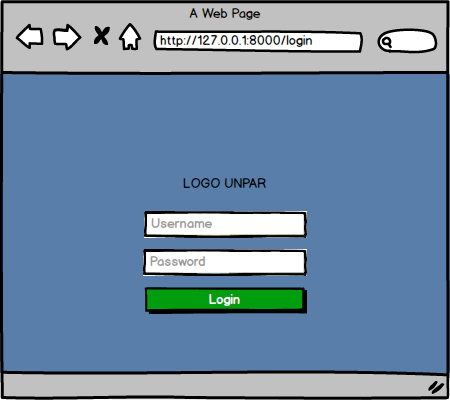
\includegraphics[scale=0.6]{F:/Skripsi/Dokumentasi_Skripsi/Gambar/Mock_Up/Login.png}
		\caption{Halaman \textit{login}}
		\label{fig:halaman_login}
	\end{figure}

\subsection{Perancangan Antar Muka Untuk Mahasiswa}
\label{sec:perancangan_antar_muka_mahasiswa}
Berdasarkan struktur modul, mahasiswa dapat menjalankan 2 fungsi yaitu membuat surat dan melihat surat yang sudah pernah dibuat yang akan dijelaskan sebagai berikut :

\begin{enumerate}
	\item Melihat surat yang sudah pernah dibuat\\
	Halaman \textit{home mahasiswa} adalah halaman yang ditampilkan apabila mahasiswa berhasil melakukan \textit{login}. Surat-surat yang pernah dibuat oleh mahasiswa ybs. akan ditampilkan pada halaman ini. Gambar \hyperlink{home_mahasiswa_yang_pernah_membuat_surat}{4.6} menunjukkan halaman \textit{home mahasiswa} yang menampilkan surat yang sudah pernah dibuat.

	\begin{figure}[H]
	\centering
		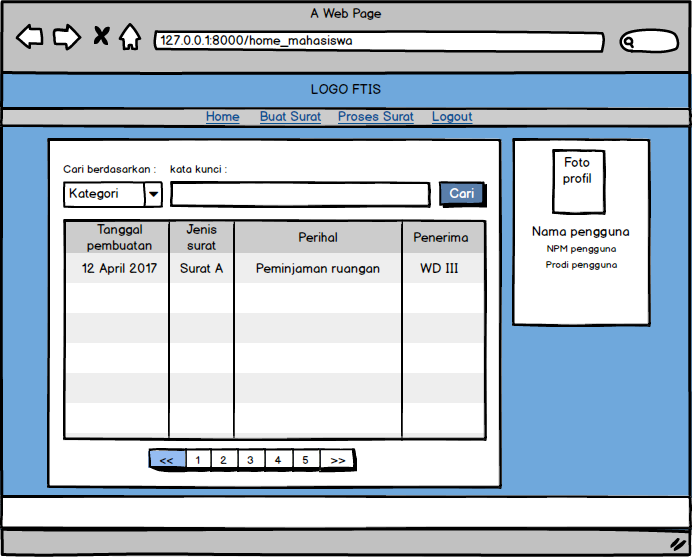
\includegraphics[scale=0.4]{F:/Skripsi/Dokumentasi_Skripsi/Gambar/Mock_Up/Mahasiswa/home_mahasiswa.png}
		\caption{Home mahasiswa yang pernah membuat surat}
		\label{fig:home_mahasiswa_yang_pernah_membuat_surat}
	\end{figure}
	
	Apabila mahasiswa ybs. belum pernah membuat surat sekalipun, maka tampilan untuk halaman \textit{home mahasiswa} akan menampilkan seperti pada gambar \hyperlink{home_mahasiswa_yang_belum_pernah_membuat_surat}{4.7} berikut.
	\begin{figure}[H]
	\centering
		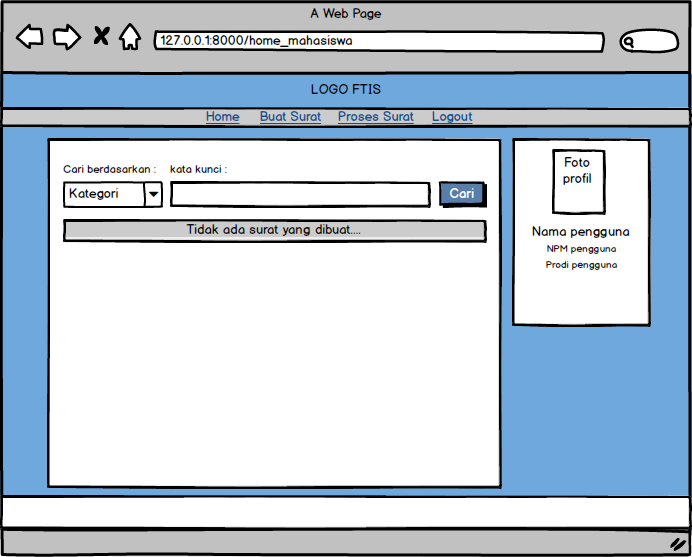
\includegraphics[scale=0.4]{F:/Skripsi/Dokumentasi_Skripsi/Gambar/Mock_Up/Mahasiswa/home_mahasiswa_kosong.png}
		\caption{Home mahasiswa yang belum pernah membuat surat}
		\label{fig:home_mahasiswa_yang_belum_pernah_membuat_surat}
	\end{figure}
	
	\item Membuat surat\\
	Untuk membuat surat mahasiswa perlu menekan menu "Buat Surat" pada \textit{navigation bar} untuk masuk ke halaman pemilihan kategori surat yang akan dibuat. Gambar \hyperlink{pilih_kategori_surat}{4.8} menunjukkan halaman pilih kategori surat.
	\begin{figure}[H]
	\centering
		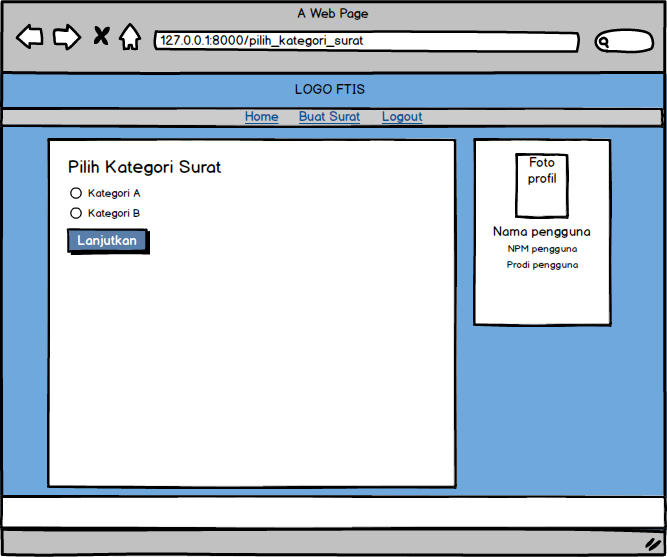
\includegraphics[scale=0.4]{F:/Skripsi/Dokumentasi_Skripsi/Gambar/Mock_Up/Mahasiswa/pilih_kategori_surat.png}
		\caption{Pilih kategori surat}
		\label{fig:pilih_kategori_surat}
	\end{figure}
	
	Setelah memilih kategori surat mahasiswa akan diarahkan ke halaman selanjutnya untuk memilih jenis surat yang akan dibuat. Gambar \hyperlink{pilih_jenis_surat}{4.9} menunjukkan halaman pilih jenis surat.
	\begin{figure}[H]
	\centering
		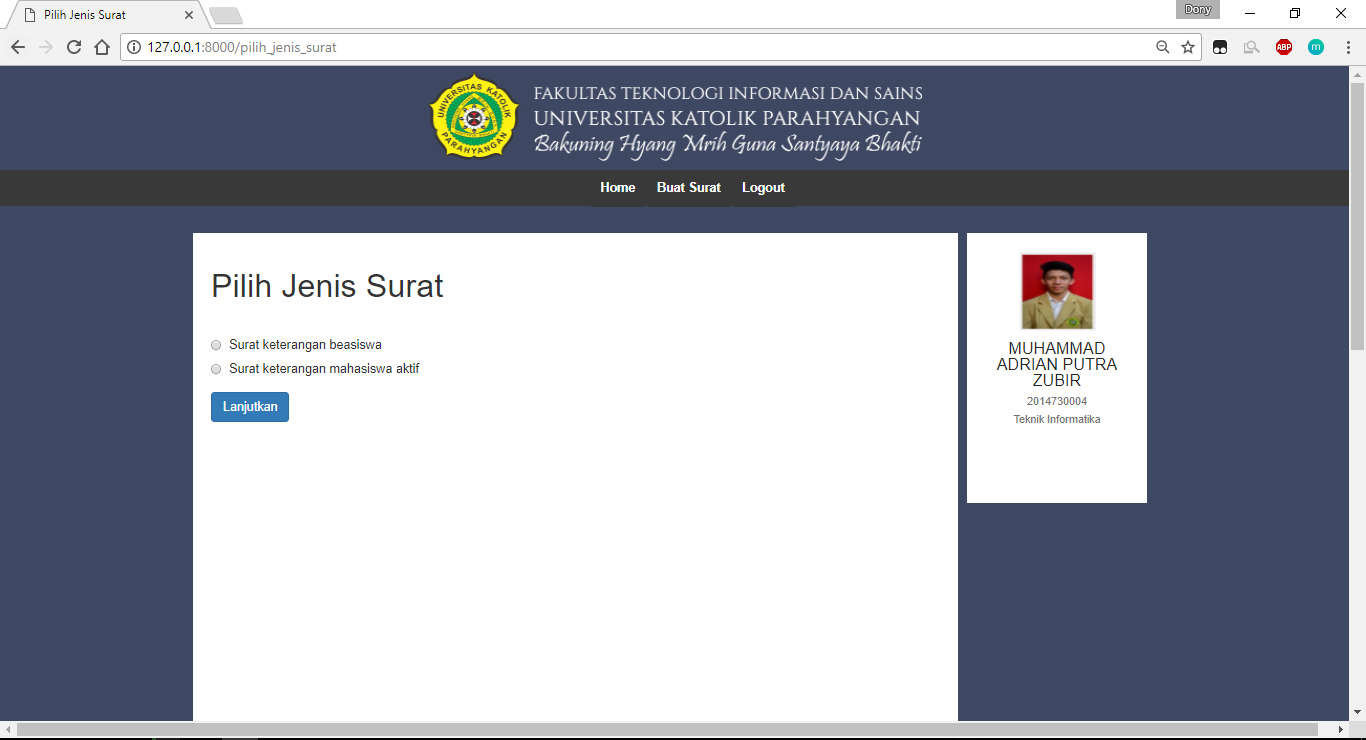
\includegraphics[scale=0.4]{F:/Skripsi/Dokumentasi_Skripsi/Gambar/Mock_Up/Mahasiswa/pilih_jenis_surat.png}
		\caption{Pilih jenis surat}
		\label{fig:pilih_jenis_surat}
	\end{figure}
	
	Setelah memilih jenis surat mahasiswa akan diarahkan ke halaman selanjutnya yaitu halaman pengisian data surat. Gambar \hyperlink{contoh_halaman_pengisian_data_surat}{4.10} menunjukkan halaman pengisian data surat.
	\begin{figure}[H]
	\centering
		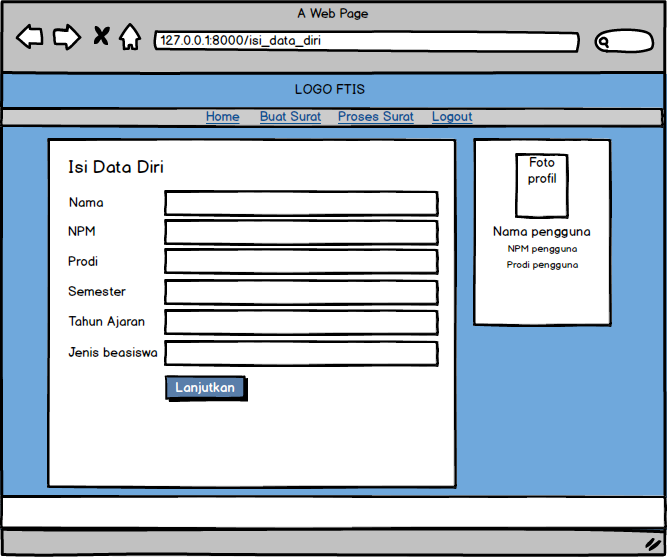
\includegraphics[scale=0.4]{F:/Skripsi/Dokumentasi_Skripsi/Gambar/Mock_Up/Mahasiswa/pengisian_data.png}
		\caption{Contoh halaman pengisian data surat}
		\label{fig:contoh_halaman_pengisian_data_surat}
	\end{figure}
	
	Apabila semua data telah diisikan pada halaman pengisian data, mahasiswa akan diarahkan ke halaman \textit{preview} untuk melihat apakah data isiannya sudah benar atau belum. Apabila data isian sudah benar mahasiswa dapat menekan tombol "Buat Surat", namun apabila ada data yang hendak diperbaiki mahasiswa dapat menekan tombol kembali. Gambar \hyperlink{contoh_halaman_preview_isi_data}{4.11} menunjukkan halaman \textit{preview} isi data surat.
	\begin{figure}[H]
	\centering
		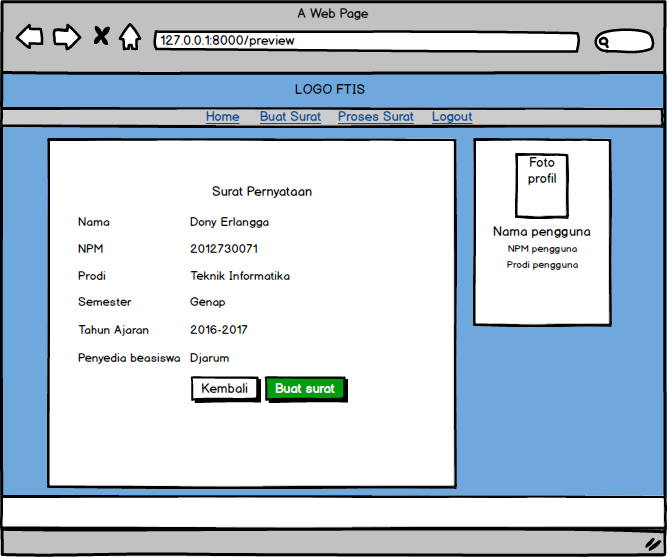
\includegraphics[scale=0.4]{F:/Skripsi/Dokumentasi_Skripsi/Gambar/Mock_Up/Mahasiswa/preview_isian_data.png}
		\caption{Contoh halaman preview isi data}
		\label{fig:contoh_halaman_preview_isi_data}
	\end{figure}
\end{enumerate}

\subsection{Perancangan Antar Muka Untuk Pejabat}
\label{sec:perancangan_antar_muka_pejabat}
Berdasarkan struktur modul, pejabat dapat menjalankan 4 fungsi yaitu melihat pesanan surat, menambahkan persetujuan dan catatan dan mengubah status penandatanganan surat yang sudah dibuat yang akan dijelaskan sebagai berikut :
\begin{enumerate}
	\item Melihat pesanan surat\\
	Surat-surat yang pernah dibuat oleh mahasiswa akan ditampilkan pada halaman \textit{home pejabat}. Gambar \hyperlink{home_pejabat_saat_ada_pesanan_surat}{4.12} menunjukkan halaman \textit{home pejabat} yang menampilkan surat yang sudah pernah dibuat.
	\begin{figure}[H]
	\centering
		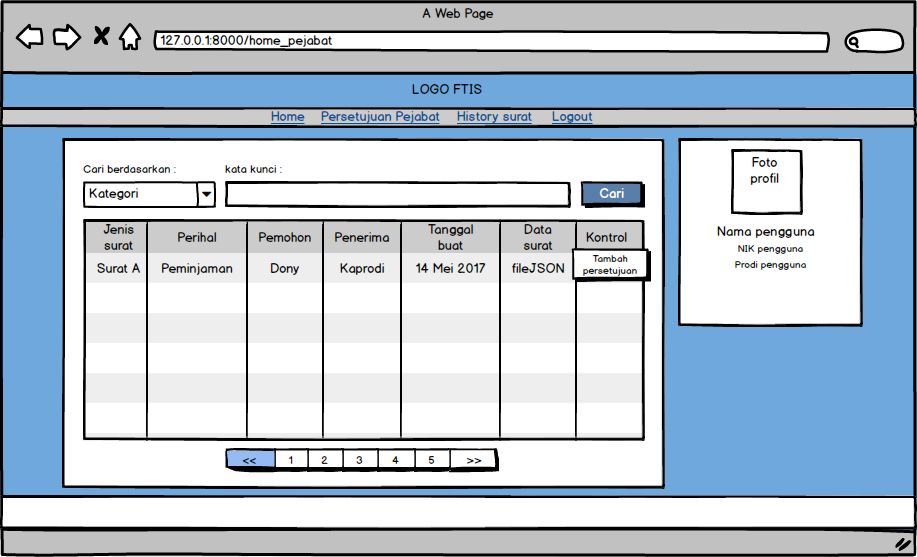
\includegraphics[scale=0.4]{F:/Skripsi/Dokumentasi_Skripsi/Gambar/Mock_Up/Pejabat/home_pejabat.png}
		\caption{Home pejabat saat ada pesanan surat}
		\label{fig:home_pejabat_saat_ada_pesanan_surat}
	\end{figure}
	
	Apabila belum ada pesanan surat, maka tampilan untuk halaman \textit{home pejabat} akan menampilkan seperti pada gambar \hyperlink{home_pejabat_saat_belum_ada_pesanan_surat}{4.13} berikut. 
	\begin{figure}[H]
	\centering
		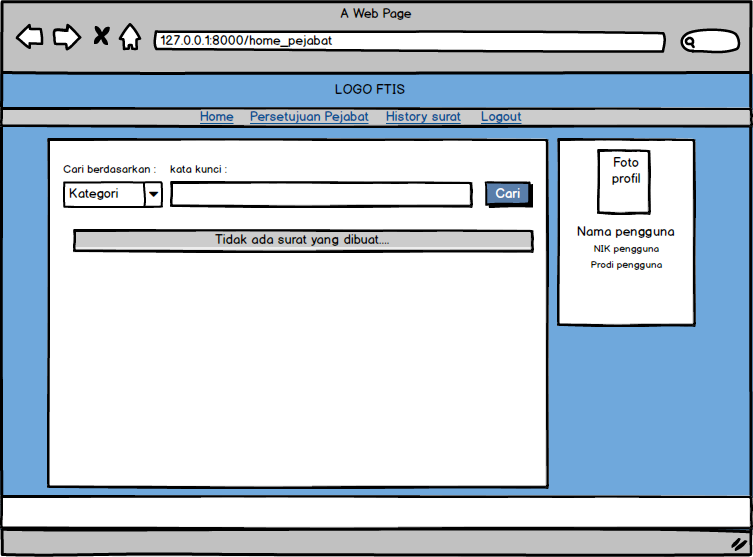
\includegraphics[scale=0.4]{F:/Skripsi/Dokumentasi_Skripsi/Gambar/Mock_Up/Pejabat/home_pejabat_kosong.png}
		\caption{Home pejabat saat belum ada pesanan surat}
		\label{fig:home_pejabat_saat_belum_ada_pesanan_surat}
	\end{figure}
	
	\item Menambahkan persetujuan dan catatan\\
	Untuk menambahkan persetujuan dan catatan pejabat perlu masuk ke halaman \textit{home pejabat} dengan menekan tombol "Home" pada \textit{navigation bar}. Pada pojok kanan tabel terdapat tombol "Tambah Catatan" yang apabila di tekan akan mengarahkan pejabat ke halaman pengisian persetujuan dan catatan. Gambar \hyperlink{halaman_pengisian_persetujuan_dan_catatan}{4.14} menunjukkan halaman pengisian persetujuan dan catatan.
	\begin{figure}[H]
	\centering
		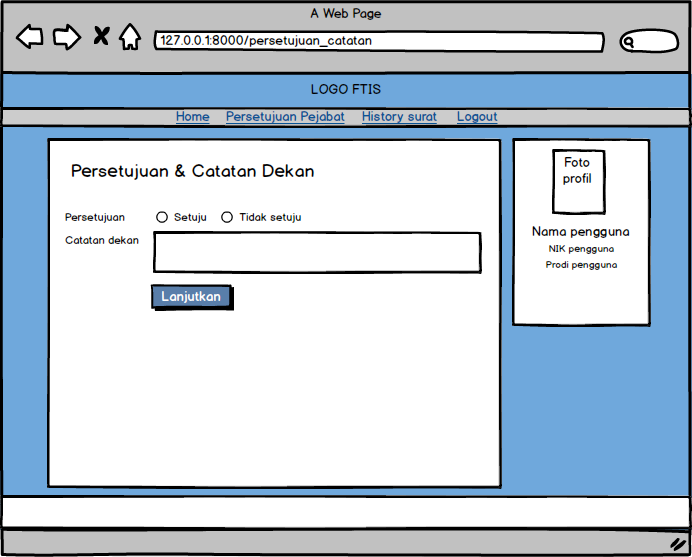
\includegraphics[scale=0.4]{F:/Skripsi/Dokumentasi_Skripsi/Gambar/Mock_Up/Pejabat/persetujuan_catatan.png}
		\caption{Halaman pengisian persetujuan dan catatan}
		\label{fig:halaman_pengisian_persetujuan_dan_catatan}
	\end{figure}
	
	Apabila persetujuan telah diisikan pada halaman pengisian persetujuan dan catatan, pejabat akan diarahkan ke halaman selanjutnya untuk melihat apakah data isiannya sudah benar atau belum. Apabila data isian sudah benar pejabat dapat menekan tombol "Kirim", namun apabila ada data yang hendak diperbaiki pejabat dapat menekan tombol kembali. Gambar \hyperlink{halaman_preview_persetujuan_dan_catatan}{4.15} menunjukkan halaman \textit{preview} persetujuan dan catatan.
	\begin{figure}[H]
	\centering
		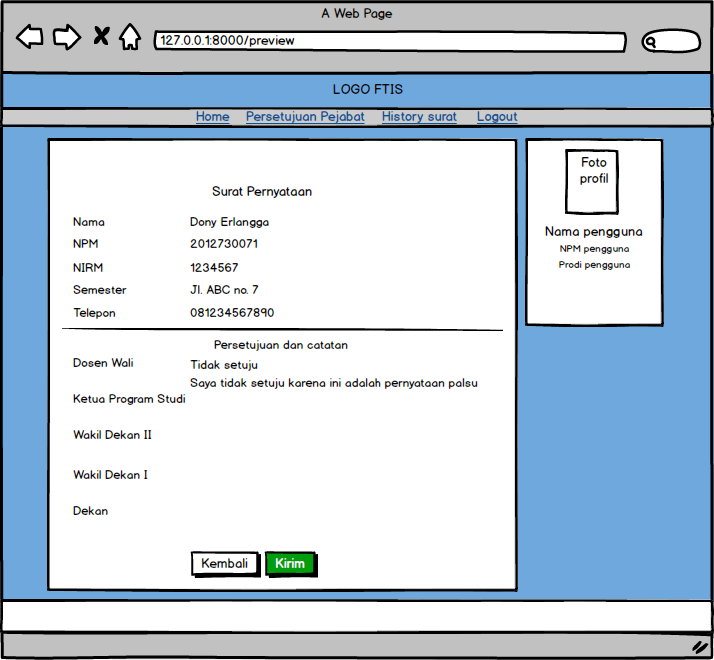
\includegraphics[scale=0.4]{F:/Skripsi/Dokumentasi_Skripsi/Gambar/Mock_Up/Pejabat/preview_persetujuan_catatan.png}
		\caption{Contoh halaman preview persetujuan dan catatan}
		\label{fig:halaman_preview_persetujuan_dan_catatan}
	\end{figure}
	
	\item Mengubah status penandatanganan surat \\
	Untuk mengubah status penandatanganan surat, petugas TU harus masuk ke halaman \textit{history} surat dan menekan tombol "Belum" pada kolom penandatanganan pada tabel \textit{history} surat. Gambar \hyperlink{halaman_history_pejabat}{4.16} merupakan halaman \textit{history} surat pada pejabat.
	\begin{figure}[H]
	\centering
		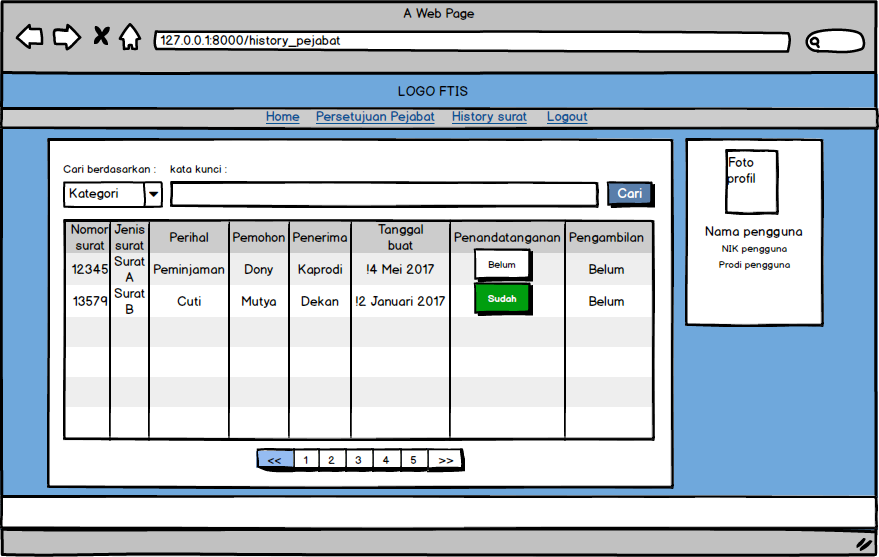
\includegraphics[scale=0.4]{F:/Skripsi/Dokumentasi_Skripsi/Gambar/Mock_Up/pejabat/history_pejabat.png}
		\caption{Halaman \textit{history} pejabat}
		\label{fig:halaman_history_pejabat}
	\end{figure}

	\item Cek persetujuan pejabat\\
	Pejabat dapat memantau proses persetujuan surat yang dipesan oleh mahasiswa bimbingannya pada halaman persetujuan pejabat yang ditampilkan pada gambar \hyperlink{halaman_persetujuan_pejabat}{4.17}.
	\begin{figure}[H]
	\centering
		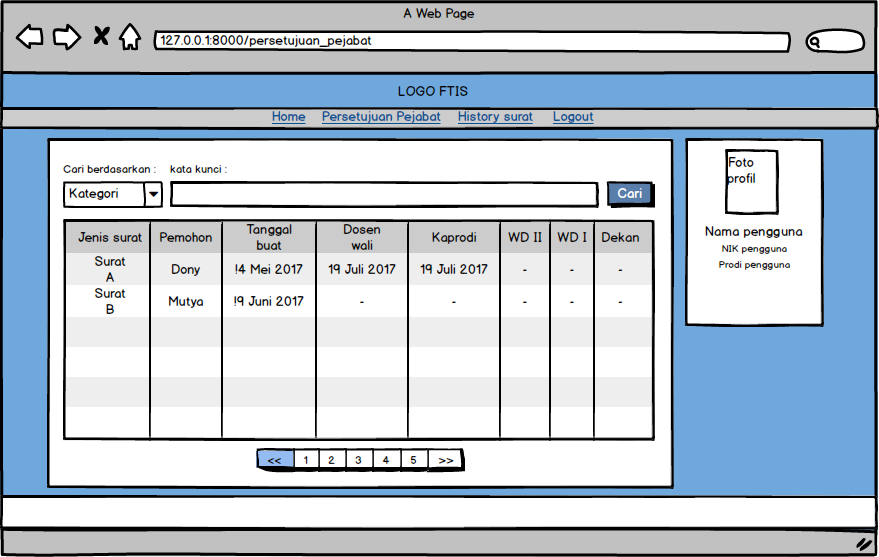
\includegraphics[scale=0.4]{F:/Skripsi/Dokumentasi_Skripsi/Gambar/Mock_Up/Pejabat/persetujuan_pejabat.png}
		\caption{Halaman persetujuan pejabat}
		\label{fig:halaman_persetujuan_pejabat}
	\end{figure}
\end{enumerate}

\subsection{Perancangan Antar Muka Untuk Petugas TU}
\label{sec:perancangan_antar_muka_petugas_tu}
Berdasarkan struktur modul, petugas TU dapat menjalankan 5 fungsi yaitu menambahkan nomor surat dan meng-\textit{generate} surat, menambahkan list data mahasiswa dan format surat baru dan mengubah status pengambilan surat yang sudah dibuat yang akan dijelaskan sebagai berikut :
\begin{enumerate}
	\item Menambahkan nomor surat dan meng-\textit{generate} surat \\
	Untuk menambahkan nomor surat dan meng-\textit{generate} surat petugas TU harus menekan tombol "Tambah Nomor Surat" pada bagian kanan tabel pesanan surat di halaman \textit{home} petugas TU. Gambar \hyperlink{halaman_home_TU}{4.18} menunjukkan halaman \textit{home} petugas TU.
	\begin{figure}[H]
	\centering
		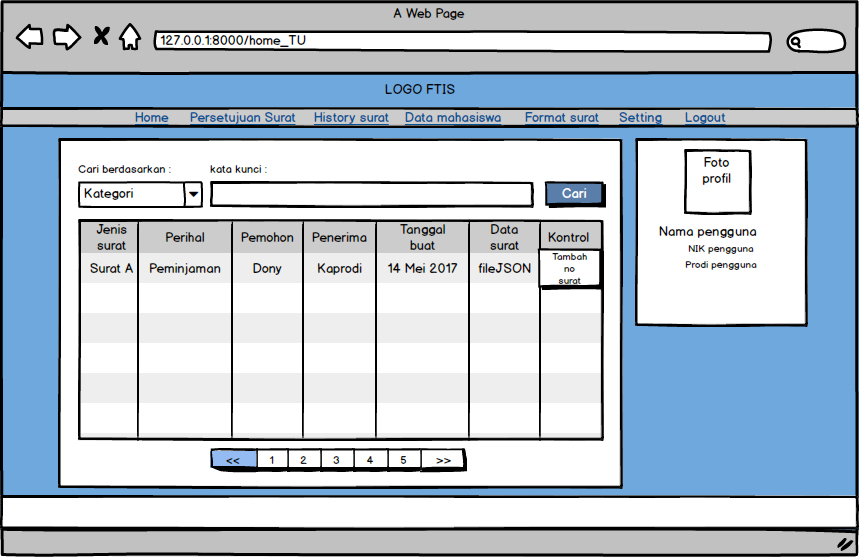
\includegraphics[scale=0.4]{F:/Skripsi/Dokumentasi_Skripsi/Gambar/Mock_Up/TU/home_TU.png}
		\caption{Halaman \textit{home} TU}
		\label{fig:halaman_home_TU}
	\end{figure}
	
	Setelah menekan tombol "Tambah Nomor Surat", petugas TU akan diarahkan menuju halaman pengisian nomor surat. Apabila nomor surat sudah diisi, petugas TU dapat menekan tombol "Buat Surat (PDF)". Gambar \hyperlink{isi_nomor_surat}{4.19} menunjukkan halaman pengisian nomor surat.
	\begin{figure}[H]
	\centering
		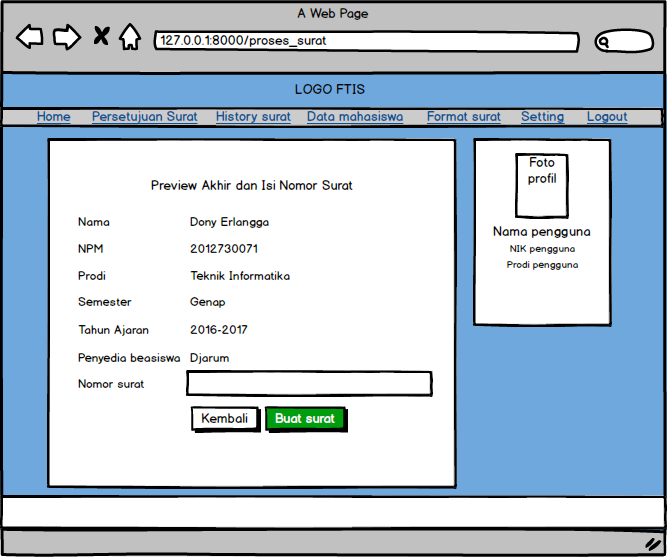
\includegraphics[scale=0.4]{F:/Skripsi/Dokumentasi_Skripsi/Gambar/Mock_Up/TU/noSurat.png}
		\caption{Halaman menambahkan nomor surat}
		\label{fig:isi_nomor_surat}
	\end{figure}
	
	\item Menambahkan format surat baru\\
	Untuk menambahkan format surat baru petugas TU harus masuk terlebih dahulu ke halaman \textit{format surat} dengan menekan tombol "Format Surat" pada \textit{navigation bar} yang ditunjukkan pada gambar \hyperlink{halaman_format_surat}{4.20}.
	\begin{figure}[H]
	\centering
		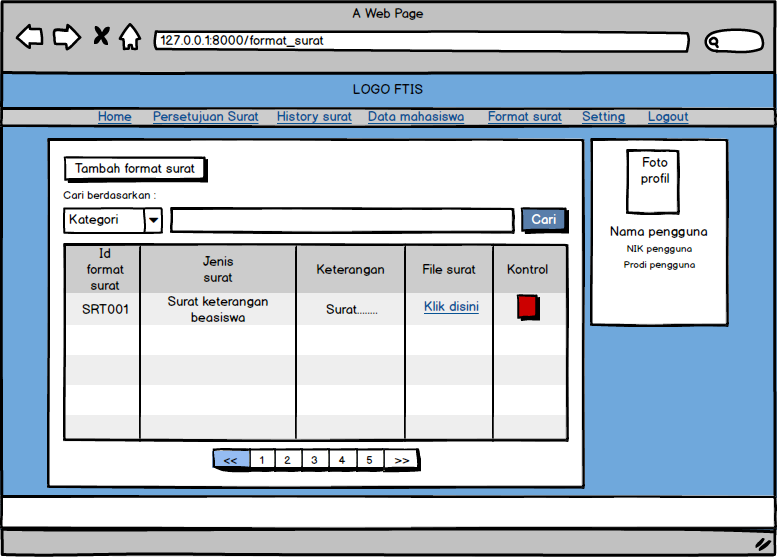
\includegraphics[scale=0.4]{F:/Skripsi/Dokumentasi_Skripsi/Gambar/Mock_Up/TU/format_surat.png}
		\caption{Halaman format surat}
		\label{fig:halaman_format_surat}
	\end{figure}
	
	Pada halaman \textit{format surat} terdapat tombol "Tambah format surat" yang apabila ditekan maka petugas TU akan diarahkan ke halaman untuk mengisi id dari format surat, nama surat, keterangan dan meng-\textit{upload} format surat baru yang ditunjukkan pada gambar \hyperlink{halaman_tambah_format_surat}{4.21}.
	\begin{figure}[H]
	\centering
		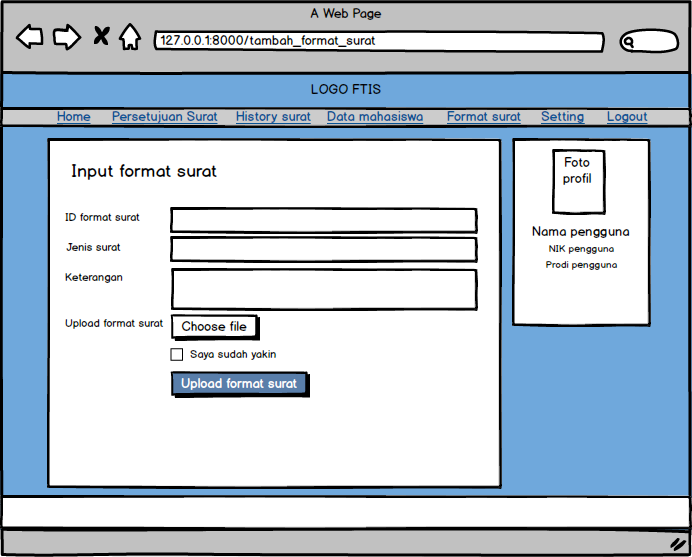
\includegraphics[scale=0.4]{F:/Skripsi/Dokumentasi_Skripsi/Gambar/Mock_Up/TU/tambah_format_surat.png}
		\caption{Halaman tambah format surat}
		\label{fig:halaman_tambah_format_surat}
	\end{figure}
	
	\item Mengubah status pengambilan surat\\
	Untuk mengubah status pengambilan surat, petugas TU harus masuk ke halaman \textit{history} surat dan menekan tombol "Belum" pada kolom pengambilan pada tabel \textit{history} surat. Gambar \hyperlink{halaman_history_TU}{4.22} merupakan halaman \textit{history} surat pada petugas TU.
	\begin{figure}[H]
	\centering
		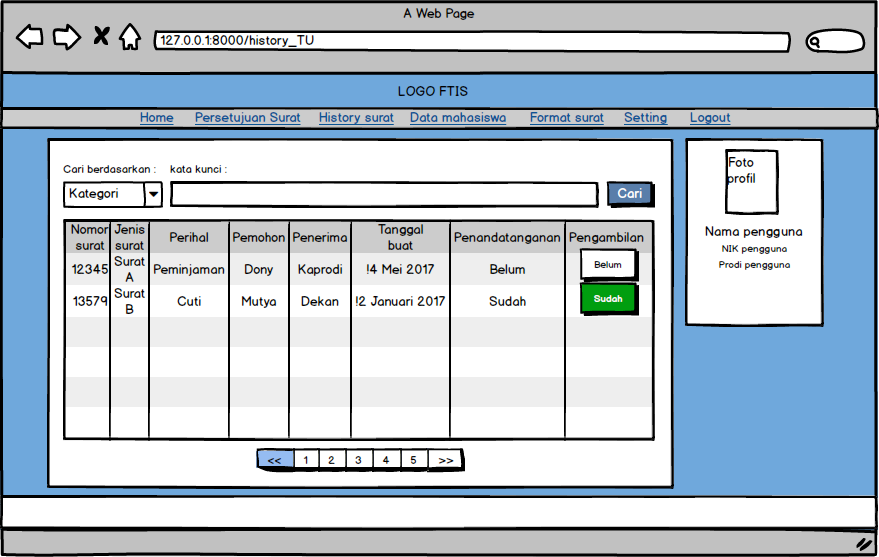
\includegraphics[scale=0.4]{F:/Skripsi/Dokumentasi_Skripsi/Gambar/Mock_Up/TU/history_TU.png}
		\caption{Halaman \textit{history} TU}
		\label{fig:halaman_history_TU}
	\end{figure}
	
	\item Mengubah semester dan tahun akademik terkini \\
	Untuk mengubah semester dan tahun akademik terkini petugas TU harus masuk terlebih dahulu ke halaman \textit{setting} dengan menekan tombol "Setting" pada \textit{navigation bar}. Gambar \hyperlink{setting}{4.23} merupakan halaman pengaturan semester dan tahun akademik.
	\begin{figure}[H]
	\centering
		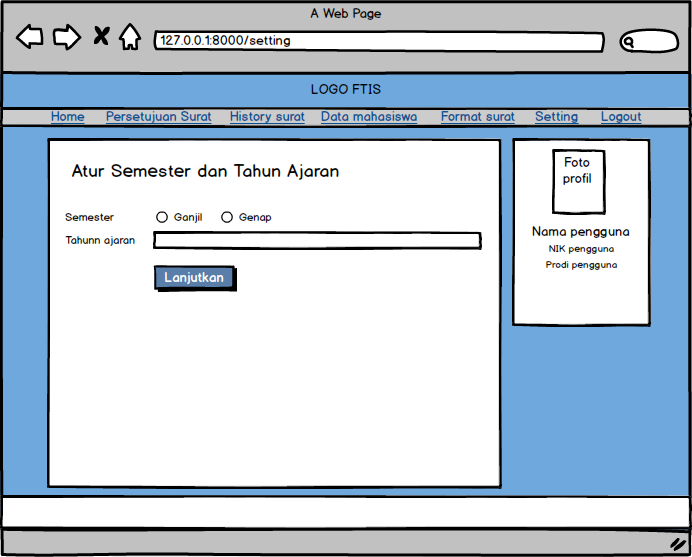
\includegraphics[scale=0.4]{F:/Skripsi/Dokumentasi_Skripsi/Gambar/Mock_Up/TU/setting.png}
		\caption{Halaman \textit{setting} semester dan tahun ajaran}
		\label{fig:setting}
	\end{figure}
	
	\item Cek persetujuan surat\\
	Petugas TU dapat memantau proses persetujuan surat yang dipesan oleh seluruh mahasiswa pada halaman persetujuan surat yang ditampilkan pada gambar \hyperlink{halaman_persetujuan_surat}{4.24}.
	\begin{figure}[H]
	\centering
		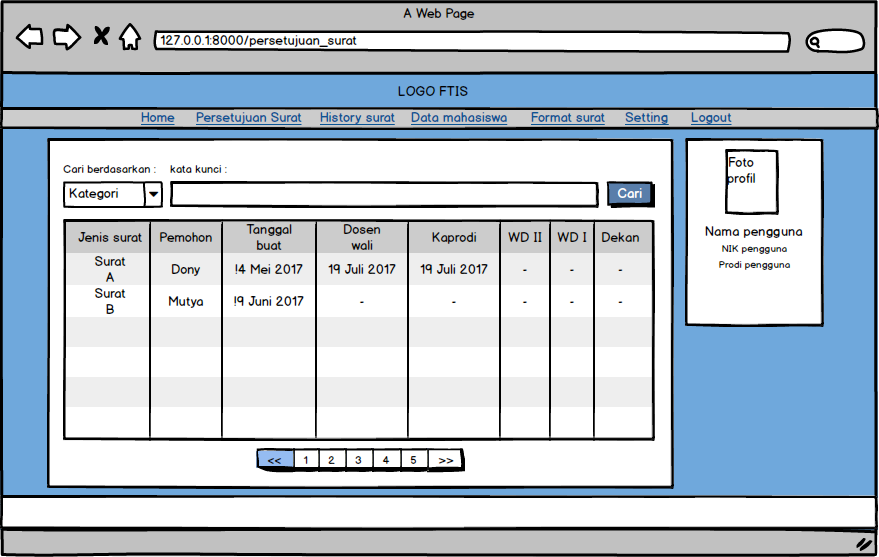
\includegraphics[scale=0.4]{F:/Skripsi/Dokumentasi_Skripsi/Gambar/Mock_Up/TU/persetujuan_surat.png}
		\caption{Halaman persetujuan surat}
		\label{fig:halaman_persetujuan_surat}
	\end{figure}
\end{enumerate}
}{}  
\ifdefstring{\vbabe}{1}{\chapter{Implementasi dan Pengujian}
\label{chap:implementasi_dan_pengujian}

\section{Lingkungan Implementasi}
\label{sec:lingkungan_implementasi}

\subsection{Lingkungan Perangkat Keras}
\label{sec:lingkungan_perangkat_keras}
Untuk membangun \textit{website} SIKSA, spesifikasi perangkat keras yang digunakan sebagai berikut :
\begin{itemize}
	\item Processor : Intel(R) Core(TM)i7-4702MQ CPU @2.20GHz
	\item Memory : DDR3 8 GB
	\item Harddisk : 1 TB
	\item VGA : Intel(R) HD Graphics 4600
\end{itemize}

\subsection{Lingkungan Perangkat Lunak}
\label{sec:lingkungan_perangkat_lunak}
Untuk membangun \textit{website} SIKSA, spesifikasi perangkat lunak yang digunakan sebagai berikut :
\begin{itemize}
	\item Web server : Apache
	\item Tools : XAMPP Control Panel v3.2.2, Atom
	\item Bahasa pemrograman : PHP, HTML, CSS
	\item Framework : Laravel 5.3
	\item Database management system : MySQL 
	\item Operation system : Windows 10 Education 64-bit
\end{itemize}

\section{Implementasi Antar Muka}
\label{sec:implementasi_antar_muka}
Berdasarkan perancangan antar muka yang telah dilakukan pada bab sebelumnya, maka dilakukan implementasi antar muka untuk setiap halaman yang terdapat pada \textit{website} SIKSA ini. Sub bagian di bawah ini menampilkan hasil \textit{screenshot} dari setiap halaman yang telah diimplementasikan berdasarkan \textit{user} yang mengakses \textit{website} SIKSA ini.

Seperti yang telah dijelaskan sebelumnya pada bagian perancangang, untuk mengakses \textit{website} SIKSA ini pengguna diharuskan melakukan \textit{login} terlebih dahulu menggunakan \textit{username} dan \textit{password} yang sesuai. Gambar \hyperlink{login}{5.1} merupakan halaman \textit{login}.
\begin{figure}[H]
	\centering
		\includegraphics[scale=0.4]{F:/Skripsi/Dokumentasi_Skripsi/Gambar/Ss/login.jpg}
		\caption{Halaman \textit{login}}
		\label{fig:login}
	\end{figure}

\subsection{Implementasi Antar Muka Untuk Mahasiswa}
\label{sec:implementasi_antar_muka_mahasiswa}
Berdasarkan perancangan antar muka untuk mahasiswa, terdapat 4 jenis halaman yang dapat diakses oleh mahasiswa. Keempat jenis halaman tersebut yaitu :
\begin{itemize}
	\item Halaman \textit{home} mahasiswa\\
	 Gambar \hyperlink{halaman_home_mahasiswa}{5.2} merupakan halaman \textit{home} mahasiswa yang menampilkan seluruh \textit{history} dari surat yang pernah dibuat oleh mahasiswa ybs. Halaman ini merupakan halaman yang pertama kali ditemukan oleh mahasiswa setelah berhasil melakukan \textit{login}.
	 \begin{figure}[H]
	\centering
		\includegraphics[scale=0.4]{F:/Skripsi/Dokumentasi_Skripsi/Gambar/Ss/Mhs/home_mhs.png}
		\caption{Halaman \textit{home} mahasiswa}
		\label{fig:halaman_home_mahasiswa}
	\end{figure}
	
	\item Halaman pilih jenis surat\\
	Gambar \hyperlink{halaman_pilih_kategori_surat}{5.3} merupakan halaman untuk pemilihan kategori surat apabila mahasiswa menekan menu "Buat Surat" pada \textit{navigation bar}.
	\begin{figure}[H]
	\centering
		\includegraphics[scale=0.4]{F:/Skripsi/Dokumentasi_Skripsi/Gambar/Ss/Mhs/pilih_kategori_surat.png}
		\caption{Halaman pilih kategori surat}
		\label{fig:halaman_pilih_kategori_surat}
	\end{figure}
	
	 \item Halaman pilih jenis surat\\
	Gambar \hyperlink{halaman_pilih_jenis_surat}{5.4} merupakan halaman untuk pemilihan jenis surat berdasarkan kategori surat yang dipilih sebelumnya.
	\begin{figure}[H]
	\centering
		\includegraphics[scale=0.4]{F:/Skripsi/Dokumentasi_Skripsi/Gambar/Ss/Mhs/pilih_jenis_surat.png}
		\caption{Halaman pilih jenis surat}
		\label{fig:halaman_pilih_jenis_surat}
	\end{figure}
	
	\item Halaman pengisian data diri\\
	Gambar \hyperlink{halaman_pengisian_data_diri}{5.5} merupakan halaman pengisian data diri berdasarkan surat yang dipilih oleh mahasiswa.
	\begin{figure}[H]
	\centering
		\includegraphics[scale=0.4]{F:/Skripsi/Dokumentasi_Skripsi/Gambar/Ss/Mhs/isi_data_diri.png}
		\caption{Halaman pengisian data diri}
		\label{fig:halaman_pengisian_data_diri}
	\end{figure}
	
	\item Halaman preview\\
	Gambar \hyperlink{halaman_preview_data_diri}{5.6} merupakan halaman untuk melihat data yang telah diisikan pada halaman pengisian data.
	\begin{figure}[H]
	\centering
		\includegraphics[scale=0.4]{F:/Skripsi/Dokumentasi_Skripsi/Gambar/Ss/Mhs/preview_data_diri.png}
		\caption{Halaman preview data diri}
		\label{fig:halaman_preview_data_diri}
	\end{figure}

\item Halaman proses surat\\
	Gambar \hyperlink{halaman_proses_surat}{5.7} merupakan halaman untuk melihat apakah surat yang sedang dipesan sudah selesai atau belum.
	\begin{figure}[H]
	\centering
		\includegraphics[scale=0.4]{F:/Skripsi/Dokumentasi_Skripsi/Gambar/Ss/Mhs/proses_surat.png}
		\caption{Halaman proses surat}
		\label{fig:halaman_proses_surat}
	\end{figure}
\end{itemize}

\subsection{Implementasi Antar Muka Untuk Petugas TU}
\label{sec:implementasi_antar_muka_petugas_tu}
Berdasarkan perancangan antar muka untuk petugas TU, terdapat 7 jenis halaman yang dapat diakses oleh petugas TU. Ketujuh jenis halaman tersebut yaitu :
\begin{itemize}
	\item Halaman \textit{home} tu
	 Gambar \hyperlink{halaman_home_tu}{5.8} merupakan halaman \textit{home} TU yang menampilkan seluruh pesanan surat. Halaman ini merupakan halaman yang pertama kali ditemukan oleh TU setelah berhasil melakukan \textit{login}.
	 \begin{figure}[H]
	\centering
		\includegraphics[scale=0.4]{F:/Skripsi/Dokumentasi_Skripsi/Gambar/Ss/TU/home_tu.png}
		\caption{Halaman \textit{home} TU}
		\label{fig:halaman_home_tu}
	\end{figure}

	\item Halaman data mahasiswa\\
	 Gambar \hyperlink{implementasi_halaman_data_mahasiswa}{5.9} merupakan halaman data mahasiswa yang menampilkan seluruh mahasiswa yang terdaftar.
	 \begin{figure}[H]
	\centering
		\includegraphics[scale=0.4]{F:/Skripsi/Dokumentasi_Skripsi/Gambar/Ss/TU/data_mahasiswa.png}
		\caption{Halaman data mahasiswa}
		\label{fig:implementasi_halaman_data_mahasiswa}
	\end{figure}
	
	\item Halaman format surat\\
	 Gambar \hyperlink{implementasi_halaman_format_surat}{5.10} merupakan halaman format surat yang menampilkan seluruh format surat yang tersedia.
	 \begin{figure}[H]
	\centering
		\includegraphics[scale=0.4]{F:/Skripsi/Dokumentasi_Skripsi/Gambar/Ss/TU/format_surat.png}
		\caption{Halaman format surat}
		\label{fig:implementasi_halaman_format_surat}
	\end{figure}
	
	\item Halaman \textit{home} mahasiswa\\
	 Gambar \hyperlink{implementasi_halaman_tambah_format_surat}{5.11} merupakan halaman untuk menambahkan format surat baru.
	 \begin{figure}[H]
	\centering
		\includegraphics[scale=0.4]{F:/Skripsi/Dokumentasi_Skripsi/Gambar/Ss/TU/tambah_format_surat.png}
		\caption{Halaman tambah format surat}
		\label{fig:implementasi_halaman_tambah_format_surat}
	\end{figure}
	
	\item Halaman \textit{history} surat\\
	 Gambar \hyperlink{halaman_history_tu}{5.12} merupakan halaman \textit{history} surat yang menampilkan seluruh \textit{history} dari surat yang pernah dibuat.
	 \begin{figure}[H]
	\centering
		\includegraphics[scale=0.4]{F:/Skripsi/Dokumentasi_Skripsi/Gambar/Ss/TU/history_tu.png}
		\caption{Halaman \textit{history} TU}
		\label{fig:halaman_history_tu}
	\end{figure}
	
	\item Halaman tambah nomor surat\\
	 Gambar \hyperlink{halaman_tambah_nomor_surat}{5.13} merupakan halaman untuk menambahkan nomor surat. Apabila nomor surat sudah diisikan, dapat menekan tombol buat surat untuk meng-\textit{generate} surat dalam bentuk \textit{file} PDF.
	 \begin{figure}[H]
	\centering
		\includegraphics[scale=0.4]{F:/Skripsi/Dokumentasi_Skripsi/Gambar/Ss/TU/tambah_noSurat.png}
		\caption{Halaman tambah nomor surat}
		\label{fig:halaman_tambah_nomor_surat}
	\end{figure}
	
	\item Halaman \textit{setting} semseter dan tahun akademik terkini\\
	 Gambar \hyperlink{halaman_setting_semester_dan_tahun_akademik_terkini}{5.14} merupakan halaman untuk mengubah semester dan tahun akademik yang berlaku untuk pada suatu semester.
	 \begin{figure}[H]
	\centering
		\includegraphics[scale=0.4]{F:/Skripsi/Dokumentasi_Skripsi/Gambar/Ss/TU/setting.png}
		\caption{Halaman \textit{setting} semester dan tahun akademik terkini}
		\label{fig:halaman_setting_semester_dan_tahun_akademik_terkini}
	\end{figure}
	
	\item Halaman persetujuan pejabat\\
	 Gambar \hyperlink{halaman_persetujuan_surat}{5.15} merupakan halaman untuk memantau proses persetujuan surat yang dipesan oleh seluruh mahasiswa.
	 \begin{figure}[H]
	\centering
		\includegraphics[scale=0.4]{F:/Skripsi/Dokumentasi_Skripsi/Gambar/Ss/TU/persetujuan_surat.png}
		\caption{Halaman persetujuan surat}
		\label{fig:halaman_persetujuan_surat}
	\end{figure}
\end{itemize}
	
\subsection{Implementasi Antar Muka Untuk Pejabat}
\label{sec:implementasi_antar_muka_pejabat}
Berdasarkan perancangan antar muka untuk pejabat, terdapat 4 jenis halaman yang dapat diakses oleh pejabat. Keempat jenis halaman tersebut yaitu :
\begin{itemize}
	\item Halaman \textit{home} pejabat\\
	 Gambar \hyperlink{halaman_home_pejabat}{5.16} merupakan halaman \textit{home} pejabat yang menampilkan seluruh pesanan surat. Halaman ini merupakan halaman yang pertama kali ditemukan oleh pejabat setelah berhasil melakukan \textit{login}.
	 \begin{figure}[H]
	\centering
		\includegraphics[scale=0.4]{F:/Skripsi/Dokumentasi_Skripsi/Gambar/Ss/Pejabat/home_pejabat.png}
		\caption{Halaman \textit{home} pejabat}
		\label{fig:halaman_home_pejabat}
	\end{figure}
	
	\item Halaman pengisian persetujuan dan catatan\\
	 Gambar \hyperlink{halaman_persetujuan_dan_catatan}{5.17} merupakan halaman pengisian persetujuan dan catatan untuk jenis surat izin cuti studi dan surat izin pengunduran diri.
	 \begin{figure}[H]
	\centering
		\includegraphics[scale=0.4]{F:/Skripsi/Dokumentasi_Skripsi/Gambar/Ss/Pejabat/tambah_persetujuan.png}
		\caption{Halaman pengisian persetujuan dan catatan}
		\label{fig:halaman_persetujuan_dan_catatan}
	\end{figure}
	
	\item Halaman \textit{preview} pengisian persetujuan dan catatan\\
	 Gambar \hyperlink{halaman_preview_persetujuan_dan_catatan}{5.18} merupakan halaman \textit{preview} pengisian persetujuan dan catatan untuk jenis surat izin cuti studi dan surat izin pengunduran diri.
	 \begin{figure}[H]
	\centering
		\includegraphics[scale=0.4]{F:/Skripsi/Dokumentasi_Skripsi/Gambar/Ss/Pejabat/preview_pejabat.png}
		\caption{Halaman \textit{preview} pengisian persetujuan dan catatan}
		\label{fig:halaman_preview_persetujuan_dan_catatan}
	\end{figure}
	
	\item Halaman persetujuan pejabat\\
	 Gambar \hyperlink{halaman_persetujuan_surat}{5.19} merupakan halaman untuk memantau proses persetujuan surat yang dipesan oleh mahasiswa yang menjadi anak bimbing dari dosen yang melakukan \textit{login} saja.
	 \begin{figure}[H]
	\centering
		\includegraphics[scale=0.4]{F:/Skripsi/Dokumentasi_Skripsi/Gambar/Ss/Pejabat/persetujuan_pejabat.png}
		\caption{Halaman persetujuan surat}
		\label{fig:halaman_persetujuan_surat}
	\end{figure}
\end{itemize}

\section{Implementasi Kode Program Untuk \textit{Compile File} Surat}
\label{sec:implementasi_kode_program_untuk_compile_file_surat}
Untuk meng-\textit{compile} \textit{file} surat dari format \textit{.tex} ke format \textit{.pdf}, digunakan fungsi yang terdapat pada \textit{file} HistorysuratController.php berikut ini.
\begin{lstlisting}[language=php, basicstyle=\tiny, caption=Fungsi untuk meng-\textit{compile} surat]
	if($request->idFormatSurat == "1"){
        $dataSurat = $request->data;
        $json = json_decode($dataSurat);
        $noSurat = $request->noSurat;
        $nama = $json->nama;
        $prodi = $this->jurusanRepo->findJurusanById($json->prodi)->nama_jurusan;
        $npm = $json->npm;
        $semester = $json->semester;
        $thnAkademik = $json->thnAkademik;
        $penyediabeasiswa = $json->penyediabeasiswa;
        $pemesan = $request->pemesan;
        
        $getLocal = getdate();
        $toString = implode(" ", $getLocal);
        $getDate = explode(" ",$toString);
        $arrTanggal = $getDate[6].'-'.$getDate[5].'-'.$getDate[3];
        $getTanggal = date_create($arrTanggal);
        $tanggal = $getTanggal->format("j F Y");

        $entry = '\mailentry{' . $noSurat . ',' . $nama . ',' . $prodi . ',' . $npm . ',' . $semester . ',' . $thnAkademik . ',' . $penyediabeasiswa . ',' . $tanggal . '}';
        $fileTemplate = file('format_surat_latex/surat_keterangan_beasiswa.tex');
        $stringFormat = "";
        $baris = count($fileTemplate);

        foreach ($fileTemplate as $line_num => $line) {
            $stringFormat .= $line;
            if($line_num == $baris-3){
                $stringFormat .= $entry;
            }
        }

        $file = fopen("arsip_surat/" . $npm . "_surat_keterangan_beasiswa.tex", "w");
        fwrite($file, $stringFormat);
        fclose($file);
        shell_exec('pdflatex -output-directory arsip_surat arsip_surat/' . $npm . '_surat_keterangan_beasiswa.tex');

        $historysurat = new Historysurat;
        $historysurat->no_surat = $noSurat;
        $historysurat->perihal = '-';
        $historysurat->penerimaSurat = $json->penyediabeasiswa;
        $historysurat->mahasiswa_id = $pemesan;
        $historysurat->formatsurat_id = $request->idFormatSurat;
        $historysurat->link_arsip_surat = 'arsip_surat/' . $npm . '_surat_keterangan_beasiswa.pdf';
        $historysurat->penandatanganan = false;
        $historysurat->pengambilan = false;
        $historysurat->save();
        return redirect('/history_TU');
      }
\end{lstlisting}

\section{Pengujian}
\label{sec:pengujian}
Bagian ini membahas mengenai pengujian fitur yang dilakukan pada \textit{website} SIKSA. Metode pengujian yang digunakan yaitu metode \textit{black box testing}, yaitu metode pengujian perangkat lunak dengan mencoba sebanyak mungkin contoh kasus ke dalam sistem tanpa melihat kode program untuk menemukan kesalahan.
\begin{itemize}
	\item Pengujian \textit{login}
	\begin{table}[H]
	\centering
	\caption{Tabel pengujian \textit{login}}
	\label{pengujian_login}
	\begin{tabular}{|l|p{6cm}|p{6cm}|}
	\hline
	\textbf{No.}&\textbf{Langkah Pengujian}&\textbf{Hasil yang Diharapkan}\\ \hline
	1&Pengguna memasukkan \textit{username} dan \textit{password} dengan benar&Pengguna berhasil masuk ke halaman \textit{home} yang sesuai dengan \textit{role}-nya \\ \hline
	2&Pengguna memasukkan \textit{username} atau \textit{password} yang salah &Pengguna akan kembali ke halaman login dan sistem mengembalikan pesan \textit{error}\\ \hline
	3&Pengguna hanya memasukkan salah satu dari \textit{username} atau \textit{password}&Pengguna akan diminta untuk mengisi bagian yang belum diisi\\ \hline
	4&Pengguna tidak memasukkan \textit{username} dan \textit{password}p{6cm}|p{6cm}&Pengguna akan diminta untuk mengisi \textit{username} dan \textit{password}\\ \hline
	\end{tabular}
	\end{table}	
	
	\item Pengujian pembuatan surat oleh mahasiswa
	\begin{table}[H]
	\centering
	\caption{Tabel pengujian pembuatan surat oleh mahasiswa}
	\label{pengujian_pembuatan_surat_oleh_mahasiswa}
	\begin{tabular}{|l|p{6cm}|p{6cm}|}
	\hline
	\textbf{No.}&\textbf{Langkah Pengujian}&\textbf{Hasil yang Diharapkan}\\ \hline
	1&Mahasiswa membuat surat keterangan beasiswa&Mahasiswa mendapatkan surat keterangan beasiswa yang sudah siap dicetak\\ \hline
	2&Mahasiswa membuat surat keterangan mahasiswa aktif&Mahasiswa mendapatkan surat keterangan mahasiswa aktif yang sudah siap dicetak\\ \hline
	3&Mahasiswa membuat surat pengantar pembuatan visa&Mahasiswa mendapatkan surat pengantar pembuatan visa yang sudah siap dicetak\\ \hline
	4&Mahasiswa membuat surat pengantar studi lapangan perorangan &Mahasiswa mendapatkan surat pengantar studi lapangan perorangan yang sudah siap dicetak\\ \hline
	5&Mahasiswa membuat surat pengantar studi lapangan untuk 2 orang &Mahasiswa mendapatkan surat pengantar studi lapangan untuk 2 orang yang sudah siap dicetak\\ \hline
	6&Mahasiswa membuat surat pengantar studi lapangan untuk 3 orang &Mahasiswa mendapatkan surat pengantar studi lapangan untuk 3 orang yang sudah siap dicetak\\ \hline
	7&Mahasiswa membuat surat pengantar studi lapangan untuk 4 orang &Mahasiswa mendapatkan surat pengantar studi lapangan untuk 4 orang yang sudah siap dicetak\\ \hline
	8&Mahasiswa membuat surat pengantar studi lapangan untuk 5 orang &Mahasiswa mendapatkan surat pengantar studi lapangan untuk 5 orang yang sudah siap dicetak\\ \hline
	9&Mahasiswa membuat surat izin cuti studi&Mahasiswa mendapatkan surat izin cuti studi yang sudah siap dicetak\\ \hline
	10&Mahasiswa membuat surat izin pengunduran diri&Mahasiswa mendapatkan surat pengunduran diri yang sudah siap dicetak\\ \hline
	\end{tabular}
	\end{table}	
	
	\begin{table}[H]
	\centering
	\begin{tabular}{|l|p{6cm}|p{6cm}|}
	\hline
	11&Mahasiswa membuat surat perwakilan perwalian untuk pengambilan 1 mata kuliah&Mahasiswa mendapatkan surat perwakilan perwalian untuk pengambilan 1 mata kuliah yang sudah siap dicetak\\ \hline
	12&Mahasiswa membuat surat perwakilan perwalian untuk pengambilan 2 mata kuliah&Mahasiswa mendapatkan surat perwakilan perwalian untuk pengambilan 2 mata kuliah yang sudah siap dicetak\\ \hline
	13&Mahasiswa membuat surat perwakilan perwalian untuk pengambilan 3 mata kuliah&Mahasiswa mendapatkan surat perwakilan perwalian untuk pengambilan 3 mata kuliah yang sudah siap dicetak\\ \hline
	14&Mahasiswa membuat surat perwakilan perwalian untuk pengambilan 4 mata kuliah&Mahasiswa mendapatkan surat perwakilan perwalian untuk pengambilan 4 mata kuliah yang sudah siap dicetak\\ \hline
	15&Mahasiswa membuat surat perwakilan perwalian untuk pengambilan 5 mata kuliah&Mahasiswa mendapatkan surat perwakilan perwalian untuk pengambilan 5 mata kuliah yang sudah siap dicetak\\ \hline
	16&Mahasiswa membuat surat perwakilan perwalian untuk pengambilan 6 mata kuliah&Mahasiswa mendapatkan surat perwakilan perwalian untuk pengambilan 6 mata kuliah yang sudah siap dicetak\\ \hline
	17&Mahasiswa membuat surat perwakilan perwalian untuk pengambilan 7 mata kuliah&Mahasiswa mendapatkan surat perwakilan perwalian untuk pengambilan 7 mata kuliah yang sudah siap dicetak\\ \hline
	18&Mahasiswa membuat surat perwakilan perwalian untuk pengambilan 8 mata kuliah&Mahasiswa mendapatkan surat perwakilan perwalian untuk pengambilan 8 mata kuliah yang sudah siap dicetak\\ \hline
	19&Mahasiswa membuat surat perwakilan perwalian untuk pengambilan 9 mata kuliah&Mahasiswa mendapatkan surat perwakilan perwalian untuk pengambilan 9 mata kuliah yang sudah siap dicetak\\ \hline
	20&Mahasiswa membuat surat perwakilan perwalian untuk pengambilan 10 mata kuliah&Mahasiswa mendapatkan surat perwakilan perwalian untuk pengambilan 10 mata kuliah yang sudah siap dicetak\\ \hline
	\end{tabular}
	\end{table}	
	
	\item Pengujian memberikan nomor surat dan \textit{generate} surat
	\begin{table}[H]
	\centering
	\caption{Tabel pengujian memberikan nomor surat dan \textit{generate} surat}
	\label{pengujian_memberikan_nomor_surat_dan_generate_surat}
	\begin{tabular}{|l|p{6cm}|p{6cm}|}
	\hline
	\textbf{No.}&\textbf{Langkah Pengujian}&\textbf{Hasil yang Diharapkan}\\ \hline
	1&Petugas TU menambahkan nomor surat&Surat bernomor\\ \hline
	\end{tabular}
	\end{table}
	
	\item Pengujian mengubah status penandatanganan surat
	\begin{table}[H]
	\centering
	\caption{Tabel pengujian mengubah status penandatanganan surat}
	\label{pengujian_mengubah_status_penandatanganan_surat}
	\begin{tabular}{|l|p{6cm}|p{6cm}|}
	\hline
	\textbf{No.}&\textbf{Langkah Pengujian}&\textbf{Hasil yang Diharapkan}\\ \hline
	1&Petugas TU menekan tombol untuk mengubah status penandatanganan surat&Status penandatanganan surat berubah menjadi "`Sudah"' \\ \hline
	\end{tabular}
	\end{table}
	
	\item Pengujian mengubah status pengambilan surat
	\begin{table}[H]
	\centering
	\caption{Tabel pengujian mengubah status pengambilan surat}
	\label{pengujian_mengubah_status_pengambilan_surat}
	\begin{tabular}{|l|p{6cm}|p{6cm}|}
	\hline
	\textbf{No.}&\textbf{Langkah Pengujian}&\textbf{Hasil yang Diharapkan}\\ \hline
	1&Petugas TU menekan tombol untuk mengubah status pengambilan surat setelah status penandatanganan surat menjadi "`Sudah"'&Status pengambilan berubah menjadi sudah \\ \hline
	2&Petugas TU menekan tombol untuk mengubah status pengambilan surat saat status penandatanganan surat masih"`Belum"'&Tombol untuk mengubah status pengambilan surat tidak bisa ditekan\\ \hline
	\end{tabular}
	\end{table} 
	
	\item Pengujian menghapus mahasiswa
	\begin{table}[H]
	\centering
	\caption{Tabel pengujian menghapus mahasiswa}
	\label{pengujian_menghapus_mahasiswa}
	\begin{tabular}{|l|p{6cm}|p{6cm}|}
	\hline
	\textbf{No.}&\textbf{Langkah Pengujian}&\textbf{Hasil yang Diharapkan}\\ \hline
	1&Petugas TU menekan tombol untuk menghapus mahasiswa&Mahasiswa terhapus \\ \hline
	\end{tabular}
	\end{table}
	
	\item Pengujian menghapus format surat
	\begin{table}[H]
	\centering
	\caption{Tabel pengujian menghapus format surat}
	\label{pengujian_menghapus_format_surat}
	\begin{tabular}{|l|p{6cm}|p{6cm}|}
	\hline
	\textbf{No.}&\textbf{Langkah Pengujian}&\textbf{Hasil yang Diharapkan}\\ \hline
	1&Petugas TU menekan tombol untuk menghapus format surat&Format surat terhapus\\ \hline
	\end{tabular}
	\end{table}
	
	\item Pengujian menambah format surat
	\begin{table}[H]
	\centering
	\caption{Tabel pengujian menambah format surat}
	\label{pengujian_menghapus_format_surat}
	\begin{tabular}{|l|p{6cm}|p{6cm}|}
	\hline
	\textbf{No.}&\textbf{Langkah Pengujian}&\textbf{Hasil yang Diharapkan}\\ \hline
	1&Petugas TU menambahkan format surat baru beserta idFormatSurat, jenis surat beserta keterangan&Format surat tersimpan di \textit{database}\\ \hline
	\end{tabular}
	\end{table}
	
	\item Pengujian mengubah semester dan tahun akademik pada setiap data mahasiswa yang terdaftar
	\begin{table}[H]
	\centering
	\caption{Tabel pengujian mengubah semester dan tahun akademik pada setiap data mahasiswa yang terdaftar}
	\label{pengujian_mengubah_semester_dan_tahun_akademik}
	\begin{tabular}{|l|p{6cm}|p{6cm}|}
	\hline
	\textbf{No.}&\textbf{Langkah Pengujian}&\textbf{Hasil yang Diharapkan}\\ \hline
	1&Petugas TU mengubah semester dan tahun akademik&\textit{Field} semester dan tahun ajaran pada tabel mahasiswa berubah sesuai dengan semester dan tahun ajaran yang dimasukkan\\ \hline
	\end{tabular}
	\end{table}
	
\end{itemize}}{}
\ifdefstring{\vbabf}{1}{\chapter{Kesimpulan dan Saran}
\label{chap:kesimpulan_dan_saran}

Pada bab ini berisi kesimpulan yang didapat setelah melakukan pembangunan \textit{website} SIKSA serta saran-saran yang dapat digunakan untuk pengembangan penelitian selanjutnya.

\section{Kesimpulan}
\label{sec:kesimpulan}
Setelah melakukan pembangunan \textit{website} SIKSA dapat ditarik beberapa kesimpulan dalam penelitian ini, yaitu :
\begin{enumerate}
	\item Telah berhasil mengidentifikasikan semua surat akademik bersama dengan kebutuhannya. Pada saat dilakukan survei didapat ada 10 surat akademik yang disediakan oleh bagian TU FTIS. Namun karena tidak semua surat tersebut menghasilkan surat yang kemudian akan dikembalikan kepada mahasiswa yang bersangkutan untuk kemudian disampaikan kepada lembaga yang membutuhkan surat tersebut. Maka didapat 6 surat yang kemudian menjadi 7 surat karena adanya surat dengan fungsi ganda.
	\item Telah berhasil mengidentifikasi dan mempelajari setiap \textit{template} surat akademik yang disediakan oleh bagian TU FTIS dan mengimplementasikan setiap \textit{template} surat akademik tersebut ke dalam format \LaTeX. Untuk beberapa format surat ada yang memiliki lebih dari 1 \textit{template} surat akademik dikarenakan ada beberapa perbedaan pada \textit{input}.
	\item Telah berhasil mengimplementasikan pembuatan surat akademik secara otomatis berdasarkan \textit{template} yang telah ditentukan. \textit{Website} yang telah dibangun mengimplementasikan konsep \textit{mailmerge} pada \LaTeX.
	\item Membangun \textit{website} yang dapat memproduksi surat akademik menggunakan \textit{framework} Laravel dan \textit{css bootstrap}. \textit{Website} yang dibangun mengadaptasi formulir isian yang sebelumnya telah digunakan sehingga tidak akan mempersulit bagi pengguna apabila hendak melakukan pemesanan surat.

\end{enumerate}

\section{Saran}
\label{sec:saran}
\textit{Website} SIKSA yang dibangun ini masih dapat dikembangkan lagi. Berdasarkan analisis \textit{website} yang dirancang, ada beberapa saran yang dapat diberikan untuk mengembangkan sistem ini, yaitu:
\begin{enumerate}
	\item Menambahkan fitur \textit{upload} data mahasiswa untuk menambahkan mahasiswa ke \textit{database}.
	\item Menambahkan foto dosen dan petugas TU pada bagian profil pengguna.
	\item Apabila \textit{website} ini hendak digunakan oleh pihak selain Fakultas Teknologi Informasi dan Sains, sebaiknya relasi TU dan fakultas pada \textit{database} dibuat terhubung agar TU hanya dari fakultas bersangkutan yang dapat melakukan pengubahan isi pada \textit{database}.
	\item Menambahkan \textit{field} kategori pada tabel format surat untuk mempermudah dalam mengkategorikan surat pada halaman "Pilih Kategori Surat" di menu milik mahasiswa.
	\item Apabila \textit{website} ini hendak digunakan oleh pihak lain selain Fakultas Teknologi Informasi dan Sains, perlu dibuatkan koneksi antara perangkat lunak dengan \textit{database} pusat yang akan digunakan.
	\item Menambahkan tabel beasiswa pada \textit{database} sehingga saat mahasiswa hendak memilih perusahaan penyedia beasiswa pada pembuatan surat keterangan beasiswa tidak terjadi kesalahan penulisan perusahaan.
	\item Memperbaiki fungsi \textit{search} yang masih belum berfungsi pada halaman \textit{home} pejabat, \textit{history} pejabat dan \textit{home} mahasiswa.  
\end{enumerate}}{}
\ifdefstring{\vbabg}{1}{\include{Bab/bab7}}{}
\ifdefstring{\vbabh}{1}{\include{Bab/bab8}}{}
\ifdefstring{\vbabi}{1}{\include{Bab/bab9}}{}

\bibliographystyle{compj} 
\bibliography{referensi}

\appendix
\apptoc 
 
\tampillmp{\vlmp}
\ifdefstring{\vlmpa}{1}{%versi 2 (8-10-2016)
\chapter{Kode Program \textit{View}}
\label{lamp:A}

%selalu gunakan single spacing untuk source code !!!!!
\singlespacing 
% language: bahasa dari kode program
% terdapat beberapa pilihan : Java, C, C++, PHP, Matlab, R, dll
%
% basicstyle : ukuran font untuk kode program
% terdapat beberapa pilihan : tiny, scriptsize, footnotesize, dll
%
% caption : nama yang akan ditampilkan di dokumen akhir, lihat contoh

\begin{lstlisting}[language=php, basicstyle=\tiny, caption=\textit{Home} mahasiswa]
	<!DOCTYPE html>
  <head>
      <title>Home - Mahasiswa</title>
      <link href="{{ asset("/bootstrap-3.3.7-dist/css/bootstrap.css") }}" rel="stylesheet" type="text/css" />
      <link href="{{ asset("/css/styles_list_surat.css") }}" rel="stylesheet" type="text/css">

  </head>

  <body>
    <div>
        <img id=banner src="{{ asset("/images/banner ftis.png") }}" />
    </div>

    <!-- Navigation here -->
    @include('mahasiswa.menu')

    <div class="container">
      <div class="main">
          <div class="row">
            <div class="col-md-8 content">
              <form class="form-inline" action= "{{ url('/data_mahasiswa') }}" method="get">
                <div class="form-group">
                  <label for="kategori_mahasiswa">Cari berdasarkan :</label><br>
                  <select name="kategori" class="form-control">
                    <option value="tanggalBuat">Cari semua surat</option>
                    <option value="tanggalBuat">Tanggal pembuatan</option>
                    <option value="perihal">Perihal</option>
                    <option value="kepada">Kepada</option>
                    <option value="jenis_surat">Jenis surat</option>
                  </select>
                </div>
                <div class="form-group">
                  <label for="searchBox">Kata kunci :</label><br>
                  <input type="text" name="searchBox" class="form-control" size="80" />
                  <button type="submit" name="findmail" class="btn btn-primary">Cari surat</button>
                </div>
              </form>
              <br>
              <table class="table table-striped">
                @if($historysurats != null)
                  @if(count($historysurats) == 0)
                      <tr>
                          <td colspan="5" align="center">Tidak ada history surat....</td>
                      </tr>
                  @else
                      <tr>
                        <th>TANGGAL PEMBUATAN</th>
                        <th>PERIHAL</th>
                        <th>KEPADA</th>
                        <th>JENIS SURAT</th>
                      </tr>
                      @foreach($historysurats as $historysurat)
                        <tr>
                          <td class="ctr">{{ $historysurat->created_at }}</td>
                          <td class="ctr">{{ $historysurat->perihal }}</td>
                          <td class="ctr">{{ $historysurat->penerimaSurat }}</td>
                          <td class="ctr">{{ $historysurat->formatsurat->jenis_surat }}</td>
                        </tr>
                      @endforeach
                  @endif
                @endif
              </table>
            </div>
            @include('mahasiswa.profile_bar')
          </div>
      </div>
    </div>
    <div class="footer">
    </div>
  </body>
</html>

\end{lstlisting}


\begin{lstlisting}[language=Java,basicstyle=\tiny,caption=Pilih kategori surat]
	
<!DOCTYPE html>
  <head>
      <title>Home</title>
      <link href="{{ asset("/bootstrap-3.3.7-dist/css/bootstrap.css") }}" rel="stylesheet" type="text/css" />
      <link href="{{ asset("/css/styles_list_surat.css") }}" rel="stylesheet" type="text/css">

  </head>

  <body>
    <div>
        <img id=banner src="{{ asset("/images/banner ftis.png") }}" />
    </div>


    <!-- Navigation Here -->
    @include('mahasiswa.menu')

    <div class="container">
      <div class="main">
        <div class="row">
          <div class="col-md-8 content">
            <h1>Pilih Kategori Surat</h1>
            <br>
            <form class="form-horizontal" action="{{ url('/pilih_jenis_surat') }}" method="post">
              <div class="form-group">
                <div class="col-sm-9">
                    <div class="radio">
                      <label>
                        <input type="radio"  name="jenis_surat" value="surat_izin" required>
                        Surat Izin
                      </label>
                    </div>
                    <div class="radio">
                      <label>
                        <input type="radio"  name="jenis_surat" value="surat_keterangan" required>
                        Surat Keterangan
                      </label>
                    </div>
                    <div class="radio">
                      <label>
                        <input type="radio"  name="jenis_surat" value="surat_perwakilan" required>
                        Surat Perwakilan
                      </label>
                    </div>
                    <div class="radio">
                      <label>
                        <input type="radio"  name="jenis_surat" value="surat_pengantar" required>
                        Surat Pengantar
                      </label>
                    </div>
                </div>
              </div>
              {!! csrf_field() !!}
              <div class="form-group">
                <div class="col-sm-6">
                  <button type="submit" class="btn btn-primary">Lanjutkan</button>
                </div>
              </div>
            </form>
          </div>
          @include('mahasiswa.profile_bar')
        </div>
      </div>
    </div>
    <div class="footer">
    </div>
  </body>
</html>

\end{lstlisting}

\begin{lstlisting}[language=Java,basicstyle=\tiny,caption=Pilih jenis surat keterangan]
	<!DOCTYPE html>
  <head>
      <title>Pilih Jenis Surat</title>
      <link href="{{ asset("/bootstrap-3.3.7-dist/css/bootstrap.css") }}" rel="stylesheet" type="text/css" />
      <link href="{{ asset("/css/styles_list_surat.css") }}" rel="stylesheet" type="text/css">

  </head>

  <body>
    <div>
        <img id=banner src="{{ asset("/images/banner ftis.png") }}" />
    </div>


    <!-- Navigation Here -->
    @include('mahasiswa.menu')

    <div class="container">
      <div class="main">
        <div class="row">
          <div class="col-md-8 content">
            <h1>Pilih Jenis Surat</h1>
            <br>
            <form class="form-horizontal" action="{{ url('/isi_data_diri') }}" method="post">
              <div class="form-group">
                <div class="col-sm-9">
                    @foreach($formatsurats as $formatsurat)
                      @if(($formatsurat->id == 1) || ($formatsurat->id == 2))
                        <div class="radio">
                          <label>
                            <input type="radio"  name="jenis_surat" value="{{ $formatsurat->id }}" required>
                            {{ $formatsurat->jenis_surat }}
                          </label>
                        </div>
                      @endif
                    @endforeach
                </div>
              </div>
              {!! csrf_field() !!}
              <div class="form-group">
                <div class="col-sm-6">
                  <button type="submit" class="btn btn-primary">Lanjutkan</button>
                </div>
              </div>
            </form>
          </div>
          @include('mahasiswa.profile_bar')
        </div>
      </div>
    </div>
    <div class="footer">
    </div>
  </body>
</html>

\end{lstlisting}

\begin{lstlisting}[language=Java,basicstyle=\tiny,caption=Pengisian data keterangan beasiswa.blade.php]
	<!DOCTYPE html>
  <head>
      <title>Isi Data Diri</title>
      <link href="{{ asset("/bootstrap-3.3.7-dist/css/bootstrap.css") }}" rel="stylesheet" type="text/css" />
      <link href="{{ asset("/css/styles_list_surat.css") }}" rel="stylesheet" type="text/css">

  </head>

  <body>
    <div>
        <img id=banner src="{{ asset("/images/banner ftis.png") }}" />
    </div>


    <!-- Navigation here -->
    @include('mahasiswa.menu')

    <div class="container">
      <div class="main">
          <div class="row">
            <div class="col-md-8 content">
              <h1>Isi Data Diri Anda</h1>
              <br>
              <form action = "{{ url('/preview') }}" method="post" class="form-horizontal">
                <div class="form-group">
                  <label for="nama" class="col-sm-3">Nama</label>
                  <div class="col-sm-9">
                    <input type="text" class="form-control" id="nama" name="nama" value="{{ $user->nama_mahasiswa }}" readonly style="border: none" />
                  </div>
                </div>
                <div class="form-group">
                  <label for="prodi" class="col-sm-3">Program studi</label>
                  <div class="col-sm-9">
                    <span type="text" class="form-control" readonly style="border: none" >{{ $user->jurusan->nama_jurusan }}</span>
                    <input type="hidden" name="prodi" value="{{ $user->jurusan_id }}"/>
                  </div>
                </div>
                <div class="form-group">
                  <label for="npm" class="col-sm-3">NPM</label>
                  <div class="col-sm-9">
                    <input type="text" class="form-control" id="npm" name="npm" value="{{ $user->npm }}" readonly style="border: none">
                  </div>
                </div>
                <div class="form-group">
                  <label for="semester" class="col-sm-3">Semester</label>
                  <div class="col-sm-9">
                    <input type="text" class="form-control" name="semester" value="{{ $user->semester }}" readonly style="border: none" />
                  </div>
                </div>
                <div class="form-group">
                  <label for="thnAkademik" class="col-sm-3">Tahun akademik</label>
                  <div class="col-sm-9">
                    <input type="text" class="form-control" name="thnAkademik" value="{{ $user->thnAkademik }}" readonly style="border: none" />
                  </div>
                </div>
                <div class="form-group">
                  <label for="penyediabeasiswa" class="col-sm-3">Penyedia beasiswa</label>
                  <div class="col-sm-9">
                    <input type="text" class="form-control" id="penyediabeasiswa" required name="penyediabeasiswa" >
                  </div>
                </div>
                <input type="hidden" value="{{ $formatsurat_id }}" name="jenis_surat">
                {!! csrf_field() !!}
                <div class="form-group">
                  <div class="col-sm-offset-3 col-sm-10">
                    <button type="submit" class="btn btn-primary">Lanjutkan</button>
                  </div>
                </div>
              </form>
            </div>
            @include('mahasiswa.profile_bar')
          </div>
      </div>
    </div>
    <div class="footer">
    </div>
  </body>
</html>

\end{lstlisting}

\begin{lstlisting}[language=Java,basicstyle=\tiny,caption=Preview isi data keterangan beasiswa]
	<!DOCTYPE html>
  <head>
      <title>Preview</title>
      <link href="{{ asset("/bootstrap-3.3.7-dist/css/bootstrap.css") }}" rel="stylesheet" type="text/css" />
      <link href="{{ asset("/css/styles_list_surat.css") }}" rel="stylesheet" type="text/css">

  </head>

  <body>
    <div>
        <img id=banner src="{{ asset("/images/banner ftis.png") }}" />
    </div>


    <!-- Navigation here -->
    @include('mahasiswa.menu')

    <div class="container">
      <div class="main">
          <div class="row">
            <div class="col-md-8 contentPreview form-horizontal">
              <h4 style="font-weight:bold">SURAT PERNYATAAN</h4>
              <br>

                <form action = "{{ url('/kirimFormulir') }}" method="post">
                  <div class="form-group">
                    <label class="col-sm-3 prevLabel">Nama</label>
                    <div class="col-sm-9" name="nama">
                        {{ $nama }}
                    </div>
                  </div>
                  <div class="form-group">
                    <label class="col-sm-3 prevLabel">Program Studi</label>
                    <div class="col-sm-9" name="prodi">
                      <span>{{ $user->jurusan->nama_jurusan }}</span>
                      <input type="hidden" name="prodi" value="{{ $prodi }}"/>
                    </div>
                  </div>
                  <div class="form-group">
                    <label class="col-sm-3 prevLabel">NPM</label>
                    <div class="col-sm-9" name="npm">
                        {{ $npm }}
                    </div>
                  </div>
                  <div class="form-group">
                    <label class="col-sm-3 prevLabel">Semester</label>
                    <div class="col-sm-9" name="semester">
                        {{ $semester }}
                    </div>
                  </div>
                  <div class="form-group">
                    <label class="col-sm-3 prevLabel">Tahun Akademik</label>
                    <div class="col-sm-9" name="thnAkademik">
                        {{ $thnAkademik }}
                    </div>
                  </div>
                  <div class="form-group">
                    <label class="col-sm-3 prevLabel">Penyedia Beasiswa</label>
                    <div class="col-sm-9" name="penyediabeasiswa">
                        {{ $penyediabeasiswa }}
                    </div>
                  </div>
                  <input type="hidden" value="{{ $formatsurat_id }}" name="idFormat">
                  <input type="hidden" value="{{ $dataSurat }}" name="dataSurat">
                  <input type="hidden" value="{{ $penyediabeasiswa }}" name="provider">
                  {!! csrf_field() !!}
                  <br>
                  <div class="form-group">
                    <div class="col-sm-offset-3 col-sm-10">
                      <button class="btn btn-default" onclick="goBack()">Kembali</button>
                      <button type="submit" class="btn btn-success">Buat Surat</button>
                    </div>
                  </div>
                </form>
            </div>
            @include('mahasiswa.profile_bar')
          </div>
      </div>
    </div>
    <div class="footer">
    </div>
    <script>
      function goBack() {
          window.history.back();
      }
    </script>
  </body>
</html>

\end{lstlisting}

\begin{lstlisting}[language=Java,basicstyle=\tiny,caption=\textit{Navigation bar} untuk mahasiswa]
	<div class="navigation">
     <div class="navbar text-center">
        <ul class="inline">
           <a href="/home_mahasiswa"><li>Home</li></a>
           <a href="/pilih_kategori_surat"><li>Buat Surat</li></a>
           <a href="{{ url('/logout') }}"
               onclick="event.preventDefault();
                        document.getElementById('logout-form').submit();"><li>
               Logout
           <form id="logout-form" action="{{ url('/logout') }}" method="POST" style="display: none;">
               {{ csrf_field() }}
           </form>
           </li></a>
        </ul>
     </div>
</div>
<br/>
<!-- <div class="row">
  <div class="col-md-offset-1 col-sm-offset-1 col-md-4 col-sm-5">
    <div style="color:white">
        Selamat Datang, {!! Auth::user()->name !!}
    </div>
  </div>
</div> -->
<div class="row">
  <div class="col-md-offset-1 col-sm-offset-1 col-sm-4 col-md-4">

  </div>
</div>

\end{lstlisting}

\begin{lstlisting}[language=Java,basicstyle=\tiny,caption=\textit{Sidebar} untuk mahasiswa]
	<div class="col-md-4 profile">
  <div class="card hovercard">
      <div class="cardheader">

      </div>
      <div class="avatar">
          <img alt="" src="{{ $user->foto_mahasiswa }}" />
      </div>
      <div class="info">
          <div class="title">
              {{ $user->nama_mahasiswa }}
          </div>
          <div class="desc">{{ $user->npm }}</div>
          <div class="desc">{{ $user->jurusan->nama_jurusan }}</div>
      </div>
  </div>
</div>

\end{lstlisting}

\begin{lstlisting}[language=Java,basicstyle=\tiny,caption=\textit{Home} pejabat]
	<!DOCTYPE html>
  <head>
      <title>Home - Pejabat</title>
      <link href="{{ asset("/bootstrap-3.3.7-dist/css/bootstrap.css") }}" rel="stylesheet" type="text/css" />
      <link href="{{ asset("/css/styles_list_surat.css") }}" rel="stylesheet" type="text/css">

  </head>

  <body>
    <div>
        <img id=banner src="{{ asset("/images/banner ftis.png") }}" />
    </div>

    <!-- Navigation Here -->
    @include('pejabat.menu')

    <div class="container">
      <div class="main">
          <div class="row">
            <div class="col-md-8 content">
              <form>
                    <table>
                      <tr>
                        <td><label>Kata kunci :</label></td>
                        <td><label>Cari berdasarkan :</label></td>
                      </tr>

                      <tr>
                        <td class = "search">
                          <select name="kategori" class="form-control">
                            <option value="tanggalBuat">Cari semua surat</option>
                            <option value="noSurat">Nomor surat</option>
                            <option value="tanggalBuat">Tanggal pembuatan</option>
                            <option value="perihal">Perihal</option>
                            <option value="kepada]">Kepada</option>
                            <option value="nama">Pembuat surat</option>
                            <option value="idFormatSurat">Jenis surat</option>
                          </select>
                        </td>
                        <td class = "search">
                          <input type="text" name="searchBox" class="form-control" size="68" />
                        </td>
                        <td>
                          <input type="submit" name="findmail" class="btn btn-primary" value="Cari surat" />
                        </td>
                      </tr>
                    </table>
              </form>
              <br>
              <table class="table table-striped">
                <tr>
                  @if(count($pesanansurats) == 0)
                    <tr>
                        <td colspan="5" align="center">Tidak ada pesanan surat ...</td>
                    </tr>
                @else
                    <tr>
                      <th>JENIS SURAT</th>
                      <th>PERIHAL</th>
                      <th>PEMOHON</th>
                      <th>PENERIMA</th>
                      <th>TANGGAL PEMBUATAN</th>
                      <th>DATA SURAT</th>
                      <th>KONTROL</th>
                    </tr>
                    @foreach($pesanansurats as $pesanansurat)
                        <tr>
                          <td class="ctr">{{ $pesanansurat->formatsurat->jenis_surat }}</td>
                          <td class="ctr">{{ $pesanansurat->perihal }}</td>
                          <td class="ctr">{{ $pesanansurat->mahasiswa->nama_mahasiswa }}</td>
                          <td class="ctr">{{ $pesanansurat->penerimaSurat }}</td>
                          <td class="ctr">{{ $pesanansurat->created_at }}</td>
                          <td class="ctr"><textarea rows="5" cols="30" style="border: none" readonly>{{ $pesanansurat->dataSurat }}</textarea></td>
                          <td class="ctr">
                            @if($pesanansurat->formatsurat->id == 9 || $pesanansurat->formatsurat->id == 10)
                            <form action="/persetujuan" method="post">
                              <input type="hidden" value="{{ $pesanansurat->formatsurat_id }}" name="idFormatSurat">
                              <input type="hidden" value="{{ $pesanansurat->dataSurat }}" name="dataSurat">
                              <input type="hidden" value="{{ $pesanansurat->id }}" name="idPesananSurat">
                              {!! csrf_field() !!}
                              <button type="submit" class="btn btn-default">Tambah<br>Persetujuan</button>
                            </form>
                            @else
                              <!-- <span class="btn btn-default"></span> -->
                            @endif
                          </td>
                        </tr>
                    @endforeach
                  @endif
              </table>
            </div>
              @include('pejabat.profile_bar')
          </div>
      </div>
    </div>
    <div class="footer">
    </div>
  </body>
</html>

\end{lstlisting}

\begin{lstlisting}[language=php,basicstyle=\tiny,caption=Tambah persetujuan dan catatan]
	<!DOCTYPE html>
  <head>
      <title>Isi Catatan Dekan</title>
      <link href="{{ asset("/bootstrap-3.3.7-dist/css/bootstrap.css") }}" rel="stylesheet" type="text/css" />
      <link href="{{ asset("/css/styles_list_surat.css") }}" rel="stylesheet" type="text/css">

  </head>

  <body>
    <div>
        <img id=banner src="{{ asset("/images/banner ftis.png") }}" />
    </div>


    <!-- Navigation Here -->
    @include('pejabat.menu')

    <div class="container">
      <div class="main">
          <div class="row">
            <div class="col-md-8 content">
              <h1>Isi Persetujuan & Catatan</h1>
              <br>
              <form class="form-horizontal" method="post" action="/previewCatatan">
                <div class="form-group">
                  <label for="persetujuan" class="col-sm-3">Persetujuan</label>
                  <div class="col-sm-9">
                    <label class="radio-inline">
                      <input type="radio" name="persetujuan" value="Setuju" checked required>Setuju
                    </label>
                    <label class="radio-inline">
                      <input type="radio" name="persetujuan" value="Tidak setuju">Tidak setuju
                    </label>
                  </div>
                </div>
                <div class="form-group">
                  <label for="catatanDekan" class="col-sm-3">Catatan (Opsional)</label>
                  <div class="col-sm-9">
                    <textarea class="form-control" id="catatan" row="5" name="catatan"></textarea>
                  </div>
                </div>
                {!! csrf_field() !!}
                <input type="hidden" value="{{ $dataSurat }}" name="dataSurat">
                <input type="hidden" value="{{ $formatsurat_id }}" name="formatsurat_id">
                <input type="hidden" value="{{ $idPesananSurat }}" name="idPesananSurat">
                <div class="form-group">
                  <div class="col-sm-offset-3 col-sm-10">
                    <button type="submit" class="btn btn-primary">Lanjutkan</button>
                  </div>
                </div>
              </form>
            </div>
            @include('pejabat.profile_bar')
          </div>
      </div>
    </div>
    <div class="footer">
    </div>
  </body>
</html>

\end{lstlisting}

\begin{lstlisting}[language=php,basicstyle=\tiny,caption=\textit{Preview} isi persetujuan dan catatan]
	<!DOCTYPE html>
  <head>
      <title>Isi data diri</title>
      <link href="{{ asset("/bootstrap-3.3.7-dist/css/bootstrap.css") }}" rel="stylesheet" type="text/css" />
      <link href="{{ asset("/css/styles_list_surat.css") }}" rel="stylesheet" type="text/css">

  </head>

  <body>
    <div>
        <img id=banner src="{{ asset("/images/banner ftis.png") }}" />
    </div>


    <!-- Navigation here -->
    @include('mahasiswa.menu')

    <div class="container">
      <div class="main">
          <div class="row">
            <div class="col-md-8 contentPreview form-horizontal">
              <h4 style="font-weight:bold">FORMULIR PERMOHONAN CUTI STUDI</h4>
              <br>
              <form action = "{{ url('/updateFormulir') }}" method="post">
                <div class="form-group">
                  <label for="nama" class="col-sm-3 prevLabel">Nama</label>
                  <div class="col-sm-9" name="nama">
                    {{ $nama }}
                  </div>
                </div>
                <div class="form-group">
                  <label for="npm" class="col-sm-3 prevLabel">NPM</label>
                  <div class="col-sm-9" name="npm">
                    {{ $npm }}
                  </div>
                </div>
                <div class="form-group">
                  <label for="prodi" class="col-sm-3 prevLabel">Program Studi</label>
                  <div class="col-sm-9" name="prodi">
                    {{ $prodi }}
                  </div>
                </div>
                <div class="form-group">
                  <label for="fakultas" class="col-sm-3 prevLabel">Fakultas</label>
                  <div class="col-sm-9" name="fakultas">
                    {{ $fakultas }}
                  </div>
                </div>
                <div class="form-group">
                  <label for="alamat" class="col-sm-3 prevLabel">Alamat</label>
                  <div class="col-sm-9" name="alamat">
                    {{ $alamat }}
                  </div>
                </div>
                <div class="form-group prev">
                  <label for="alasanCutiStudi" class="col-sm-3 prevLabel">Alasan cuti studi ke </label>
                  <div class="col-sm-9" name="alasanCutiStudi">
                    {{ $cutiStudiKe }}<br>
                    {{ $alasanCutiStudi }}
                  </div>
                </div>
                <div class="form-group prev">
                  <label for="catatanDosenWali" class="col-sm-3 prevLabel">Catatan dosen wali </label>
                  <div class="col-sm-9" name="catatanDosenWali">
                    Nama : {{ $dosenWali }}<br>
                    {{ $persetujuanDosenWali }}<br>
                    {{ $catatanDosenWali }}
                    <input type="hidden" name="dosenWali" value="{{ $persetujuanDosenWali }}|{{ $catatanDosenWali }}" />
                  </div>
                </div>
                <div class="form-group prev">
                  <label for="catatanKaprodi" class="col-sm-3 prevLabel">Catatan Kaprodi </label>
                  <div class="col-sm-9" name="catatanKaprodi">
                    {{ $persetujuanKaprodi }}<br>
                    {{ $catatanKaprodi }}
                    <input type="hidden" name="kaprodi" value="{{ $persetujuanKaprodi }}|{{ $catatanKaprodi }}" />
                  </div>
                </div>
                <div class="form-group prev">
                  <label for="catatanWDII" class="col-sm-3 prevLabel">Catatan WD II</label>
                  <div class="col-sm-9" name="catatanWDII">
                    {{ $persetujuanWDII }}<br>
                    {{ $catatanWDII }}
                    <input type="hidden" name="wd2" value="{{ $persetujuanWDII }}|{{ $catatanWDII }}" />
                  </div>
                </div>
                <div class="form-group prev">
                  <label for="catatanWDI" class="col-sm-3 prevLabel">Catatan WD I</label>
                  <div class="col-sm-9" name="catatanWDI">
                    {{ $persetujuanWDI }}<br>
                    {{ $catatanWDI }}
                    <input type="hidden" name="wd1" value="{{ $persetujuanWDI }}|{{ $catatanWDI }}" />
                  </div>
                </div>
                <div class="form-group prev">
                  <label for="persetujuanDekan" class="col-sm-3 prevLabel">Persetujuan Dekan</label>
                  <div class="col-sm-9" name="persetujuanDekan" >
                    {{ $persetujuanDekan }}
                    <input type="hidden" name="dekan" value="{{ $persetujuanDekan }}" />
                  </div>
                </div>
                <div class="form-group prev">
                  <label for="semester" class="col-sm-3 prevLabel">Semester</label>
                  <div class="col-sm-9" name="semester">
                    {{ $semester }}
                  </div>
                </div>
                <div class="form-group prev">
                  <label for="thnAkademik" class="col-sm-3 prevLabel">Tahun Akademik</label>
                  <div class="col-sm-9" name="thnAkademik">
                    {{ $thnAkademik }}
                  </div>
                </div>
                <input type="hidden" value="{{ $formatsurat_id }}" name="idFormat">
                <input type="hidden" value="{{ $dataSurat }}" name="dataSurat">
                <input type="hidden" name="idPesanansurat" value="{{$idPesanansurat}}">

                {!! csrf_field() !!}
                <br>
                <div class="form-group">
                  <div class="col-sm-offset-3 col-sm-10">
                    <button class="btn btn-default" onclick="goBack()">Kembali</button>
                    <button type="submit" class="btn btn-success">Buat Surat</button>
                  </div>
                </div>
              </form>
            </div>
            @include('mahasiswa.profile_bar')
          </div>
      </div>
    </div>
    <div class="footer">
    </div>
    <script>
      function goBack() {
          window.history.back();
      }
    </script>
  </body>
</html>
	
\end{lstlisting}

\begin{lstlisting}[language=php,basicstyle=\tiny,caption=\textit{History} pejabat]
	<!DOCTYPE html>
  <head>
      <title>Data Mahasiswa</title>
      <link href="{{ asset("/bootstrap-3.3.7-dist/css/bootstrap.css") }}" rel="stylesheet" type="text/css" />
      <link href="{{ asset("/css/styles_list_surat.css") }}" rel="stylesheet" type="text/css">
  </head>

  <body>
    <div>
        <img id=banner src="{{ asset("/images/banner ftis.png") }}" />
    </div>

    <!-- Navigation Here -->
    @include('pejabat.menu')

    <div class="container">
      <div class="main">
          <div class="row">
            <div class="col-md-8 content">
              <form class="form-inline" action= "{{ url('/format_surat') }}" method="get">
                <div class="form-group">
                  <label for="kategori_format_surat">Cari berdasarkan :</label><br>
                  <select name="kategori_mahasiswa" class="form-control">
                    <option value="">Cari semua surat</option>
                    <option value="noSurat">Nomor Surat</option>
                    <option value="jenis_surat">Jenis Surat</option>
                    <option value="perihal">Perihal</option>
                    <option value="pemohon">Pemohon</option>
                    <option value="penerima">Penerima</option>
                    <option value="tanggalPembuatan">Tanggal Pembuatan</option>
                  </select>
                </div>
                <div class="form-group">
                  <label for="searchBox_format_surat">Kata kunci :</label><br>
                  <input type="text" name="searchBox" class="form-control" size="68" />
                  <button type="submit" name="findmail" class="btn btn-primary">Cari surat</button>
                </div>
              </form>
              <br>
              <table class="table table-striped table-hover">
                @if($historysurats != null)
                  @if(count($historysurats) == 0)
                      <tr>
                          <td colspan="5" align="center">Tidak ada history surat....</td>
                      </tr>
                  @else
                      <tr>
                        <th>NOMOR SURAT</th>
                        <th>JENIS SURAT</th>
                        <th>PERIHAL</th>
                        <th>PEMOHON</th>
                        <th>PENERIMA</th>
                        <th>TANGGAL PEMBUATAN</th>
                        <th>PENANDATANGANAN</th>
                        <th>PENGAMBILAN</th>
                      </tr>
                      @foreach($historysurats as $historysurat)
                        <tr>
                          <td class="ctr">{{ $historysurat->no_surat }}</td>
                          <td class="ctr">{{ $historysurat->formatsurat->jenis_surat }}</td>
                          <td class="ctr">{{ $historysurat->perihal }}</td>
                          <td class="ctr">{{ $historysurat->mahasiswa->nama_mahasiswa  }}</td>
                          <td class="ctr">{{ $historysurat->penerimaSurat }}</td>
                          <td class="ctr">{{ $historysurat->created_at }}</td>
                          <td align="center">
                            @if($historysurat->penandatanganan)
                              <button type="submit" disabled class="btn btn-success" style="display:block">Sudah</button>
                            @else
                              <form action="{{url('/ubahStatusPenandatanganan')}}" method="post">
                                <input type="hidden" value="{{ $historysurat->id }}" name="id">
                                {!! csrf_field() !!}
                                <button type="submit" class="btn btn-default " style="display:block">Belum</button>
                              </form>
                            @endif
                          </td>
                          <td class="ctr">
                            @if($historysurat->pengambilan)
                              <p>Sudah</p>
                            @else
                              <p>Belum</p>
                            @endif
                          </td>
                        </tr>
                      @endforeach
                  @endif
                @endif
              </table>
              <div style="text-align:center">{!! $historysurats->links() !!}</div>
            </div>
            @include('pejabat.profile_bar')
          </div>
      </div>
    </div>
    <div class="footer">
    </div>
  </body>
</html>

\end{lstlisting}

\begin{lstlisting}[language=php,basicstyle=\tiny,caption=\textit{Navigation bar} untuk pejabat]
	<div class="navigation">
     <div class="navbar text-center">
        <ul class="inline">
          <a href="/home_pejabat"><li>Home</li></a>
          <a href="/history_pejabat"><li>History Surat</li></a>

          <a href="{{ url('/logout') }}"
              onclick="event.preventDefault();
                       document.getElementById('logout-form').submit();"><li>
              Logout
          <form id="logout-form" action="{{ url('/logout') }}" method="POST" style="display: none;">
              {{ csrf_field() }}
          </form>
          </li></a>
        </ul>
     </div>
</div>
<br>
<!-- <div class="row">
  <div class="col-md-offset-1 col-sm-offset-1 col-md-4 col-sm-5">
    <div style="color:white">
        Selamat Datang, {!! Auth::user()->name !!}
    </div>
  </div>
</div> -->
<div class="row">
  <div class="col-md-offset-1 col-sm-offset-1 col-sm-4 col-md-4">

  </div>
</div>

\end{lstlisting}

\begin{lstlisting}[language=php,basicstyle=\tiny,caption=\textit{Sidebar} untuk pejabat]
	<div class="col-md-4 profile">
  <div class="card hovercard">
      <div class="cardheader">

      </div>
      <div class="avatar">
          <img alt="" src="http://simpleicon.com/wp-content/uploads/user1.png">
      </div>
      <div class="info">
          <div class="title">
              {{ $user->nama_dosen }}
          </div>
          <div class="desc">{{ $user->nik }}</div>
          <div class="desc">{{ $user->jurusan->nama_jurusan }}</div>
      </div>
  </div>
</div>

\end{lstlisting}

\begin{lstlisting}[language=php,basicstyle=\tiny,caption=\textit{Home} TU]
	<!DOCTYPE html>
  <head>
      <title>Home - TU</title>
      <link href="{{ asset("/bootstrap-3.3.7-dist/css/bootstrap.css") }}" rel="stylesheet" type="text/css" />
      <link href="{{ asset("/css/styles_list_surat.css") }}" rel="stylesheet" type="text/css">

  </head>

  <body>
    <div>
        <img id=banner src="{{ asset("/images/banner ftis.png") }}" />
    </div>

    @include('tu.menu')

    <div class="container">
      <div class="main">
          <div class="row">
            <div class="col-md-8 content">
              <form class="form-inline" action= "{{ url('/home_TU') }}" method="get">
                <div class="form-group">
                  <label for="kategori">Cari berdasarkan :</label><br>
                  <select name="kategori" class="form-control">
                    <option value="">Cari semua surat</option>
                    <option value="jenis_surat">Jenis Surat</option>
                    <option value="perihal">Perihal</option>
                    <option value="pemohonSurat">Pemohon Surat</option>
                    <option value="penerimaSurat">Penerima Surat</option>
                    <option value="tanggalBuat">Tanggal pembuatan</option>
                  </select>
                </div>
                <div class="form-group">
                  <label for="searchBox">Kata kunci :</label><br>
                  <input type="text" name="searchBox" class="form-control" size="69" />
                  <button type="submit" name="findmail" class="btn btn-primary">Cari surat</button>
                </div>
              </form>
              <br>
              <table class="table table-striped">
                @if(count($pesanansurats) == 0)
                    <tr>
                        <td colspan="5" align="center">Tidak ada pesanan surat ...</td>
                    </tr>
                @else
                    <tr>
                      <th>JENIS SURAT</th>
                      <th>PERIHAL</th>
                      <th>PEMOHON</th>
                      <th>PENERIMA</th>
                      <th>TANGGAL PEMBUATAN</th>
                      <th>DATA SURAT</th>
                      <th>KONTROL</th>
                    </tr>
                    @foreach($pesanansurats as $pesanansurat)
                        <tr>
                          <td class="ctr">{{ $pesanansurat->formatsurat->jenis_surat }}</td>
                          <td class="ctr">{{ $pesanansurat->perihal }}</td>
                          <td class="ctr">{{ $pesanansurat->mahasiswa->nama_mahasiswa }}</td>
                          <td class="ctr">{{ $pesanansurat->penerimaSurat }}</td>
                          <td class="ctr">{{ $pesanansurat->created_at }}</td>
                          <td class="ctr"><textarea rows="5" cols="30" style="border: none" readonly>{{ $pesanansurat->dataSurat }}</textarea></td>
                          <td class="ctr">
                            <form action="/proses_surat" method="post">
                              <input type="hidden" value="{{ $pesanansurat->id }}" name="id">
                              <input type="hidden" value="{{ $pesanansurat->formatsurat_id }}" name="idFormatSurat">
                              <input type="hidden" value="{{ $pesanansurat->dataSurat }}" name="prosesSurat">
                              {!! csrf_field() !!}
                              <button type="submit" class="btn btn-default">Tambah<br>Nomor<br>Surat</button>
                            </form>
                          </td>
                        </tr>
                    @endforeach
                  @endif
              </table>
              <div style="text-align:center">{!! $pesanansurats->links() !!}</div>
            </div>
          @include('tu.profile_bar')
          </div>
      </div>
    </div>
    <div class="footer">
        <div style="text-align:center">Copyright Dony Erlangga</div>
    </div>
  </body>
</html>

\end{lstlisting}

\begin{lstlisting}[language=php,basicstyle=\tiny,caption=Tambah nomor surat untuk surat keterangan beasiswa]
	<!DOCTYPE html>
  <head>
      <title>Tambah Nomor Surat & Generate PDF</title>
      <link href="{{ asset("/bootstrap-3.3.7-dist/css/bootstrap.css") }}" rel="stylesheet" type="text/css" />
      <link href="{{ asset("/css/styles_list_surat.css") }}" rel="stylesheet" type="text/css">

  </head>

  <body>
    <div>
        <img id=banner src="{{ asset("/images/banner ftis.png") }}" />
    </div>

    @include('tu.menu')

    <div class="container">
      <div class="main">
          <div class="row">
            <div class="col-md-8 content">
                <h3 style="font-weight:bold;">Preview Akhir dan Isi Nomor Surat</h3>
                <br>
                <form class="form-horizontal" action="{{ url('/generatePDF') }}" method="post">
                  <div class="form-group">
                    <label class="col-sm-3 prevLabel">Nama</label>
                    <div class="col-sm-9" name="nama">
                        {{ $nama }}
                    </div>
                  </div>
                  <div class="form-group">
                    <label class="col-sm-3 prevLabel">Program Studi</label>
                    <div class="col-sm-9" name="prodi">
                      <span>{{ $user->jurusan->nama_jurusan }}</span>
                      <input type="hidden" name="prodi" value="{{ $prodi }}"/>
                    </div>
                  </div>
                  <div class="form-group">
                    <label class="col-sm-3 prevLabel">NPM</label>
                    <div class="col-sm-9" name="npm">
                        {{ $npm }}
                    </div>
                  </div>
                  <div class="form-group">
                    <label class="col-sm-3 prevLabel">Semester</label>
                    <div class="col-sm-9" name="semester">
                        {{ $semester }}
                    </div>
                  </div>
                  <div class="form-group">
                    <label class="col-sm-3 prevLabel">Tahun Akademik</label>
                    <div class="col-sm-9" name="thnAkademik">
                        {{ $thnAkademik }}
                    </div>
                  </div>
                  <div class="form-group">
                    <label class="col-sm-3 prevLabel">Jenis Beasiswa</label>
                    <div class="col-sm-9" name="penyediabeasiswa">
                        {{ $penyediabeasiswa }}
                    </div>
                  </div>
                  <div class="form-group">
                      <label class="col-sm-3" for="noSurat">Nomor Surat</label>
                      <div class="col-sm-6">
                          <input type="text" class="form-control" name="noSurat" required />
                      </div>
                  </div>
                  <input type="hidden" value="{{ $dataSurat }}" id="format" name="data">
                  <input type="hidden" value="{{ $formatsurat_id }}" name="idFormatSurat">
                  <input type="hidden" value="{{ $pemesan }}" name="pemesan">
                  {!! csrf_field() !!}
                  <br>
                  <div class="form-group">
                    <div class="col-sm-offset-3 col-sm-10">
                      <button class="btn btn-default" onclick="goBack()">Kembali</button>
                      <button type="submit" class="btn btn-success">Buat Surat (PDF)</button>
                    </div>
                  </div>
                </form>
            </div>
            @include('tu.profile_bar')
          </div>
      </div>
    </div>
    <div class="footer">
         
    </div>
    <script>
      function goBack() {
          window.history.back();
      }

      function compile(){
        var pdftex = new PDFTeX();
        var latex_code =
      }
    </script>
  </body>
</html>
\end{lstlisting}

\begin{lstlisting}[language=php,basicstyle=\tiny,caption=\textit{History} TU]
	<!DOCTYPE html>
  <head>
      <title>History Surat - TU</title>
      <link href="{{ asset("/bootstrap-3.3.7-dist/css/bootstrap.css") }}" rel="stylesheet" type="text/css" />
      <link href="{{ asset("/css/styles_list_surat.css") }}" rel="stylesheet" type="text/css" />
  </head>

  <body>
    <div>
        <img id=banner src="{{ asset("/images/banner ftis.png") }}" />
    </div>

    @include('tu.menu')

    <div class="container">
      <div class="main">
          <div class="row">
            <div class="col-md-8 content">
              <form class="form-inline" action= "{{ url('/format_surat') }}" method="get">
                <div class="form-group">
                  <label for="kategori_format_surat">Cari berdasarkan :</label><br>
                  <select name="kategori_mahasiswa" class="form-control">
                    <option value="">Cari semua surat</option>
                    <option value="noSurat">Nomor Surat</option>
                    <option value="jenis_surat">Jenis Surat</option>
                    <option value="perihal">Perihal</option>
                    <option value="pemohon">Pemohon</option>
                    <option value="penerima">Penerima</option>
                    <option value="tanggalPembuatan">Tanggal Pembuatan</option>
                  </select>
                </div>
                <div class="form-group">
                  <label for="searchBox_format_surat">Kata kunci :</label><br>
                  <input type="text" name="searchBox" class="form-control" size="68" />
                  <button type="submit" name="findmail" class="btn btn-primary">Cari surat</button>
                </div>
              </form>
              <br>
              <table class="table table-striped table-hover">
                @if($historysurats != null)
                  @if(count($historysurats) == 0)
                      <tr>
                          <td colspan="5" align="center">Tidak ada history surat....</td>
                      </tr>
                  @else
                      <tr>
                        <th>NOMOR SURAT</th>
                        <th>JENIS SURAT</th>
                        <th>PERIHAL</th>
                        <th>PEMOHON</th>
                        <th>PENERIMA</th>
                        <th>TANGGAL PEMBUATAN</th>
                        <th>PENANDATANGANAN</th>
                        <th>PENGAMBILAN</th>
                      </tr>
                      @foreach($historysurats as $historysurat)
                        <tr>
                          <td class="ctr">{{ $historysurat->no_surat }}</td>
                          <td class="ctr">{{ $historysurat->formatsurat->jenis_surat }}</td>
                          <td class="ctr">{{ $historysurat->perihal }}</td>
                          <td class="ctr">{{ $historysurat->mahasiswa->nama_mahasiswa }}</td>
                          <td class="ctr">{{ $historysurat->penerimaSurat }}</td>
                          <td class="ctr">{{ $historysurat->created_at }}</td>
                          <td class="ctr">
                            @if($historysurat->penandatanganan)
                              <p>Sudah</p>
                            @else
                              <p>Belum</p>
                            @endif
                          </td>
                          <td align="center">
                            @if($historysurat->pengambilan)
                              <button type="submit" disabled class="btn btn-success">Sudah</button>
                            @else
                              @if($historysurat->penandatanganan == false)
                                <button type="submit" disabled class="btn btn-default">Belum</button>
                              @else
                                <form method="post" action="{{url('/ubahStatusPengambilan')}}">
                                  <input type="hidden" value="{{ $historysurat->id }}" name="id">
                                  {!! csrf_field() !!}
                                  <button type="submit" class="btn btn-default">Belum</button>
                                </form>
                              @endif
                            @endif
                          </td>
                        </tr>
                      @endforeach
                  @endif
                @endif
              </table>
              <div style="text-align:center">{!! $historysurats->links() !!}</div>
            </div>
              @include('tu.profile_bar')
          </div>
      </div>
    </div>
    <div class="footer">
         
    </div>
  </body>
</html>
\end{lstlisting}

\begin{lstlisting}[language=php,basicstyle=\tiny,caption=Data mahasiswa]
	<!DOCTYPE html>
  <head>
      <title>Data Mahasiswa</title>
      <link href="{{ asset("/bootstrap-3.3.7-dist/css/bootstrap.css") }}" rel="stylesheet" type="text/css" />
      <link href="{{ asset("/css/styles_list_surat.css") }}" rel="stylesheet" type="text/css">

  </head>

  <body>
    <div>
        <img id=banner src="{{ asset("/images/banner ftis.png") }}" />
    </div>

      @include('tu.menu')

    <div class="container">
      <div class="main">
          <div class="row">
            <div class="col-md-8 content">
              <!-- <a href="{{ URL::to('/tambah_data_mahasiswa') }}" class="btn btn-default">Tambah Data Mahasiswa</a> -->
              <form class="form-inline" action= "{{ url('/data_mahasiswa') }}" method="get">
                <div class="form-group">
                  <label for="kategori_mahasiswa">Cari berdasarkan :</label><br>
                  <select name="kategori_mahasiswa" class="form-control">
                    <option value="tanggalBuat">Cari semua surat</option>
                    <option value="nirm">NIRM</option>
                    <option value="npm">NPM</option>
                    <option value="nama_mahasiswa">Nama Mahasiswa</option>
                    <option value="prodi">Program Studi</option>
                    <option value="angkatan">Angkatan</option>
                    <option value="kota_lahir">Kota Lahir</option>
                    <option value="tanggal_lahir">Tanggal Lahir</option>
                  </select>
                </div>
                <div class="form-group">
                  <label for="searchBox">Kata kunci :</label><br>
                  <input type="text" name="searchBox" class="form-control" size = "65">
                  <button type="submit" name="findmail" class="btn btn-primary">Cari mahasiswa</button>
                </div>
              </form>
              <br>
              <table class="table table-striped table-hover">
                @if(count($mahasiswas) == 0)
                    <tr>
                        <td colspan="5" align="center">Tidak ada data mahasiswa ...</td>
                    </tr>
                @else
                    <tr>
                      <th>NIRM</th>
                      <th>NPM</th>
                      <th>NAMA MAHASISWA</th>
                      <th>PROGRAM STUDI</th>
                      <th>ANGKATAN</th>
                      <th>KOTA LAHIR</th>
                      <th>TANGGAL LAHIR</th>
                      <th>DOSEN WALI</th>
                      <th>FOTO</th>
                      <th>KONTROL</th>
                    </tr>
                    @foreach($mahasiswas as $mahasiswa)
                      <tr>
                        <td class="ctr">{{ $mahasiswa->nirm }}</td>
                        <td class="ctr">{{ $mahasiswa->npm }}</td>
                        <td class="ctr">{{ $mahasiswa->nama_mahasiswa }}</td>
                        <td class="ctr">{{ $mahasiswa->jurusan->nama_jurusan }}</td>
                        <td class="ctr">{{ $mahasiswa->angkatan }}</td>
                        <td class="ctr">{{ $mahasiswa->kota_lahir }}</td>
                        <td class="ctr">{{ $mahasiswa->tanggal_lahir }}</td>
                        <td class="ctr">{{ $mahasiswa->dosen->nama_dosen }}</td>
                        <td style="text-align:center"><a href = "{{ $mahasiswa->foto }}">klik disini</a></td>
                        <td>
                          <form action="/hapusMahasiswa" method="post">
                            <input type="hidden" value="{{ $mahasiswa->id }}" name="deleteID">
                            {!! csrf_field() !!}
                            <button type="submit" class="btn btn-danger" aria-label="Remove" data-toggle="tooltip" title="Remove">
                                <span class="glyphicon glyphicon-remove" aria-hidden="true"></span>
                            </button>
                          </form>
                        </td>
                      </tr>
                    @endforeach
                @endif
              </table>
            </div>
            @include('tu.profile_bar')
          </div>
      </div>
    </div>
    <div class="footer">
    </div>
  </body>
</html>

\end{lstlisting}

\begin{lstlisting}[language=php,basicstyle=\tiny,caption=Format surat]
	
<!DOCTYPE html>
  <head>
      <title>Format Surat</title>
      <link href="{{ asset("/bootstrap-3.3.7-dist/css/bootstrap.css") }}" rel="stylesheet" type="text/css" />
      <link href="{{ asset("/css/styles_list_surat.css") }}" rel="stylesheet" type="text/css" />
      <script src="{{ asset("/js/jquery-3.2.0.min.js") }}" type="text/javascript"></script>

  </head>

  <body>
    <div>
        <img id=banner src="{{ asset("/images/banner ftis.png") }}" />
    </div>

    @include('tu.menu')

    <div id="myModal" class="modal">
      <div class="modal-content" id="show">
        <span class="close">&times;</span>
      </div>
    </div>
    <div class="container">
      <div class="main">
          <div class="row">
            <div class="col-md-8 content" id ="test">
              <a href="{{ URL::to('/tambah_format_surat') }}" class="btn btn-default">Tambah Format Surat</a>
              <form class="form-inline" action= "{{ url('/format_surat') }}" method="get">
                <div class="form-group">
                  <label for="kategori_format_surat">Cari berdasarkan :</label><br>
                  <select name="kategori_format_surat" class="form-control">
                    <option value="">Cari semua surat</option>
                    <option value="idFormatSurat">ID Format Surat</option>
                    <option value="jenis_surat">Jenis Surat</option>
                    <option value="keterangan">Keterangan</option>
                  </select>
                </div>
                <div class="form-group">
                  <label for="searchBox_format_surat">Kata kunci :</label><br>
                  <input type="text" name="searchBox_format_surat" class="form-control" size = "65">
                  <button type="submit" name="findmail" class="btn btn-primary">Cari format surat</button>
                </div>
              </form>
              <br>
              <table class="table table-striped table-hover">
                @if($formatsurats != null)
                  @if(count($formatsurats) == 0)
                      <tr>
                          <td colspan="5" align="center">Tidak ada format surat ...</td>
                      </tr>
                  @else
                      <tr>
                        <th>ID FORMAT SURAT</th>
                        <th>JENIS SURAT</th>
                        <th>KETERANGAN</th>
                        <th>FILE SURAT</th>
                        <th colspan ="2"> KONTROL</th>
                      </tr>
                      @foreach($formatsurats as $formatsurat)
                        <tr>
                          <td class="ctr">{{ $formatsurat->idFormatSurat }}</td>
                          <td class="ctr">{{ $formatsurat->jenis_surat }}</td>
                          <td class="ctr">{{ $formatsurat->keterangan }}</td>
                          <td class="ctr">
                              <button type="submit" onclick="showModal({{ $formatsurat->id }})" class="btn btn-link">Klik disini</button>
                          </td>
                          <td class="ctr">
                            <form action="/hapusFormatsurat" method="post">
                              <input type="hidden" value="{{ $formatsurat->id }}" name="deleteID">
                              {!! csrf_field() !!}
                              <button type="submit" class="btn btn-danger" aria-label="Remove" data-toggle="tooltip" title="Remove">
                                  <span class="glyphicon glyphicon-remove" aria-hidden="true"></span>
                              </button>
                            </form>
                          </td>
                        </tr>
                      @endforeach
                  @endif
                @endif
              </table>
              <div style="text-align:center">{!! $formatsurats->links() !!}</div>
            </div>
            @include('tu.profile_bar')
          </div>
      </div>
    </div>
    <div class="footer">
    </div>
    <script type="text/javascript" src="{{ asset("js/jquery-3.2.0.min.js") }}"></script>
    <script>
        // Get the modal
        var modal = document.getElementById('myModal');
        var btn = document.getElementById("showFormatID");
        var span = document.getElementsByClassName("close")[0];

        function tutup() {
            modal.style.display = "none";
        }

        window.onclick = function(event) {
            if (event.target == modal) {
                modal.style.display = "none";
            }
        }
        function showModal(id){
          var jqxhr = $.get( "http://127.0.0.1:8000/Api/showFormatSurat?id=" + id, function() {
          })
          .done(function(data) {
            document.getElementById("show").innerHTML = `<span onclick='tutup()' class='close'>&times;</span>` + data.stringFormat;
            // $('#myModal').css({'position' : 'fixed'});
            modal.style.display = "block";
            modal.style.position = "fixed";
            // $('#test').css('position' : 'fixed');
          })
          .fail(function(error) {
            alert( "Error : " + error);
          });
        }
    </script>
  </body>
</html>

\end{lstlisting}

\begin{lstlisting}[language=php,basicstyle=\tiny,caption=Tambah format surat]
	
<!DOCTYPE html>
  <head>
      <title>Data Mahasiswa</title>
      <link href="{{ asset("/bootstrap-3.3.7-dist/css/bootstrap.css") }}" rel="stylesheet" type="text/css" />
      <link href="{{ asset("/css/styles_list_surat.css") }}" rel="stylesheet" type="text/css">

  </head>

  <body>
    <div>
        <img id=banner src="{{ asset("/images/banner ftis.png") }}" />
    </div>

      @include('tu.menu')

    <div class="container">
      <div class="main">
          <div class="row">
            <div class="col-md-8 content">
              <h1>Input Format Surat</h1>
              <br><br>
              <form class="form-horizontal" action="{{ url('/uploadFormat')}}" method="post"  enctype="multipart/form-data">
                <div class="form-group">
                  <label for="idFormatSurat" class="col-sm-3">ID Format Surat</label>
                  <div class="col-sm-9">
                    <input type="text" class="form-control" id="idFormatSurat" name="idFormatSurat" required>
                  </div>
                </div>
                <div class="form-group">
                  <label for="jenis_surat" class="col-sm-3">Jenis Surat</label>
                  <div class="col-sm-9">
                    <input type="text" class="form-control" id="jenis_surat" name="jenis_surat" required />
                  </div>
                </div>
                <div class="form-group">
                  <label class="col-sm-3" for="keterangan">Keterangan</label>
                  <div class="col-sm-9">
                    <textarea class="form-control" row="3" id="keterangan" name="keterangan" required></textarea>
                  </div>
                </div>
                <div class="form-group">
                  <label for="nama" class="col-sm-3">Upload Format Surat</label>
                  <div class="col-sm-9">
                    <input type="file" class="form-control" name="uploadFormat" required />
                  </div>
                </div>
                <div class="form-group">
                  <div class="col-sm-3"></div>
                  <div class="col-sm-9 checkbox">
                    <label><input type="checkbox" required/> Saya sudah yakin</label>
                  </div>
                </div>
                {!! csrf_field() !!}
                <div class="form-group">
                  <div class="col-sm-3"></div>
                  <div class="col-sm-9">
                    <button type="submit" class="btn btn-primary">Upload format surat (.TeX)</button>
                  </div>
                </div>
              </form>
            </div>
            @include('tu.profile_bar')
          </div>
      </div>
    </div>
    <div class="footer">
    </div>
  </body>
</html>

\end{lstlisting}

\begin{lstlisting}[language=php,basicstyle=\tiny,caption=\textit{Setting} semester dan thnAjaran.blade.php]
	<!DOCTYPE html>
  <head>
      <title>Setting</title>
      <link href="{{ asset("/bootstrap-3.3.7-dist/css/bootstrap.css") }}" rel="stylesheet" type="text/css" />
      <link href="{{ asset("/css/styles_list_surat.css") }}" rel="stylesheet" type="text/css">

  </head>

  <body>
    <div>
        <img id=banner src="{{ asset("/images/banner ftis.png") }}" />
    </div>

    @include('tu.menu')
      <div class="container">
        <div class="main">
            <div class="row">
              <div class="col-md-8 content">
                <h1>Atur Semester dan Tahun Ajaran</h1>
                <br>
                <form class="form-horizontal" method="post" action="/updateSemester">
                  <div class="form-group">
                    <label for="persetujuan" class="col-sm-3">Semester</label>
                    <div class="col-sm-9">
                      <label class="radio-inline">
                        <input type="radio" name="semester" value="Ganjil" checked required>Ganjil
                      </label>
                      <label class="radio-inline">
                        <input type="radio" name="semester" value="Genap">Genap
                      </label>
                    </div>
                  </div>
                  <div class="form-group">
                    <label for="catatanDekan" class="col-sm-3">Tahun Akademik</label>
                    <div class="col-sm-9">
                      <input type="text" class="form-control" name="thnAkademik">
                    </div>
                  </div>
                  {!! csrf_field() !!}
                  <div class="form-group">
                    <div class="col-sm-offset-3 col-sm-10">
                      <button type="submit" class="btn btn-primary">Lanjutkan</button>
                    </div>
                  </div>
                </form>
              </div>
              @include('tu.profile_bar')
            </div>
        </div>
      </div>
      <div class="footer">
      </div>
    </body>
  </html>

\end{lstlisting}

\begin{lstlisting}[language=php,basicstyle=\tiny,caption=\textit{Navigation bar} untuk petugas TU]
	<div class="navigation">
         <div class="navbar text-center">
            <ul class="inline">
               <a href="/home_TU"><li>Home</li></a>
               <a href="/history_TU"><li>History Surat</li></a>
               <a href="/data_mahasiswa"><li>Data Mahasiswa</li></a>
               <a href="/format_surat"><li>Format Surat</li></a>
               <a href="/setting"><li>Setting</li></a>
           <a href="{{ url('/logout') }}"
               onclick="event.preventDefault();
                        document.getElementById('logout-form').submit();"><li>
               Logout
           <form id="logout-form" action="{{ url('/logout') }}" method="POST" style="display: none;">
               {{ csrf_field() }}
           </form>
           </li></a>
        </ul>
     </div>
</div>
<br/>
<!-- <div class="row">
  <div class="col-md-offset-1 col-sm-offset-1 col-md-4 col-sm-5">
    <div style="color:white">
        Selamat Datang, {!! Auth::user()->name !!}
    </div>
  </div>
</div> -->
<div class="row">
  <div class="col-md-offset-1 col-sm-offset-1 col-sm-4 col-md-4">

  </div>
</div>

\end{lstlisting}

\begin{lstlisting}[language=php,basicstyle=\tiny,caption=\textit{Sidebar} untuk petugas TU]
	<div class="col-md-4 profile">
  <div class="card hovercard">
      <div class="cardheader">

      </div>
      <div class="avatar">
          <img alt="" src="http://simpleicon.com/wp-content/uploads/user1.png">
      </div>
      <div class="info">
          <div class="title">
              {{ $user->namaTU }}
          </div>
          <div class="desc">{{ $user->NIK }}</div>
      </div>
  </div>
</div>

\end{lstlisting}

\begin{lstlisting}[language=Java,basicstyle=\tiny,caption=Persetujuan surat]
<!DOCTYPE html>
  <head>
      <title>Persetujuan - TU</title>
      <link href="{{ asset("/bootstrap-3.3.7-dist/css/bootstrap.css") }}" rel="stylesheet" type="text/css" />
      <link href="{{ asset("/css/styles_list_surat.css") }}" rel="stylesheet" type="text/css">

  </head>

  <body>
    <div>
        <img id=banner src="{{ asset("/images/banner ftis.png") }}" />
    </div>

    @include('tu.menu')

    <div class="container">
      <div class="main">
          <div class="row">
            <div class="col-md-8 content">
              <form class="form-inline" action= "{{ url('/home_TU') }}" method="get">
                <div class="form-group">
                  <label for="kategori">Cari berdasarkan :</label><br>
                  <select name="kategori" class="form-control">
                    <option value="">Cari semua surat</option>
                    <option value="jenis_surat">Jenis surat</option>
                    <option value="pemohonSurat">Pemohon surat</option>
                    <option value="penerimaSurat">Penerima surat</option>
                  </select>
                </div>
                <div class="form-group">
                  <label for="searchBox">Kata kunci :</label><br>
                  <input type="text" name="searchBox" class="form-control" size="69" />
                  <button type="submit" name="findmail" class="btn btn-primary">Cari surat</button>
                </div>
              </form>
              <br>
              <table class="table table-striped">
                @if(count($pesanansurats) == 0)
                    <tr>
                        <td colspan="5" align="center">Tidak ada pesanan surat ...</td>
                    </tr>
                @else
                    <tr>
                        <th>JENIS SURAT</th>
                        <th>PEMOHON</th>
                        <th>TANGGAL PEMBUATAN</th>
                        <th>DOSEN WALI</th>
                        <th>KAPRODI</th>
                        <th>WD II</th>
                        <th>WD I</th>
                        <th>DEKAN</th>
                    </tr>
                    @foreach($pesanansurats as $pesanansurat)
                        <tr>
                          <td class="ctr">{{ $pesanansurat->formatsurat->jenis_surat }}</td>
                          <td class="ctr">{{ $pesanansurat->mahasiswa->nama_mahasiswa }}</td>
                          <td class="ctr">{{ $pesanansurat->created_at }}</td>
                          <td class="ctr">
                            @if($pesanansurat->tglDosenWali)
                                {{ $pesanansurat->tglDosenWali }}
                            @else
                                -
                            @endif
                          </td>
                          <td class="ctr">
                            @if($pesanansurat->tglKaprodi)
                                {{ $pesanansurat->tglKaprodi }}
                            @else
                                -
                            @endif
                          </td>
                          <td class="ctr">
                            @if($pesanansurat->tglWDII)
                                {{ $pesanansurat->tglWDII }}
                            @else
                                -
                            @endif
                          </td>
                          <td class="ctr">
                            @if($pesanansurat->tglWDI)
                                {{ $pesanansurat->tglWDI }}
                            @else
                                -
                            @endif
                          </td>
                          <td class="ctr">
                            @if($pesanansurat->tglDekan)
                                {{ $pesanansurat->tglDekan }}
                            @else
                                -
                            @endif
                          </td>
                        </tr>
                    @endforeach
                  @endif
              </table>
              <div style="text-align:center">{!! $pesanansurats->links() !!}</div>
            </div>
          @include('tu.profile_bar')
          </div>
      </div>
    </div>
    <div class="footer">
        <div style="text-align:center">Copyright Dony Erlangga</div>
    </div>
  </body>
</html>

\end{lstlisting}

\begin{lstlisting}[language=Java,basicstyle=\tiny,caption=Persetujuan pejabat]
<!DOCTYPE html>
  <head>
      <title>Persetujuan - Pejabat</title>
      <link href="{{ asset("/bootstrap-3.3.7-dist/css/bootstrap.css") }}" rel="stylesheet" type="text/css" />
      <link href="{{ asset("/css/styles_list_surat.css") }}" rel="stylesheet" type="text/css">

  </head>

  <body>
    <div>
        <img id=banner src="{{ asset("/images/banner ftis.png") }}" />
    </div>

    @include('pejabat.menu')

    <div class="container">
      <div class="main">
          <div class="row">
            <div class="col-md-8 content">
              <form class="form-inline" action= "{{ url('/persetujuan_surat') }}" method="get">
                <div class="form-group">
                  <label for="kategori">Cari berdasarkan :</label><br>
                  <select name="kategori" class="form-control">
                    <option value="">Cari semua surat</option>
                    <option value="jenis_surat">Jenis surat</option>
                    <option value="pemohonSurat">Pemohon surat</option>
                    <option value="penerimaSurat">Penerima surat</option>
                  </select>
                </div>
                <div class="form-group">
                  <label for="searchBox">Kata kunci :</label><br>
                  <input type="text" name="searchBox" class="form-control" size="69" />
                  <button type="submit" name="findmail" class="btn btn-primary">Cari surat</button>
                </div>
              </form>
              <br>
              <table class="table table-striped">
                @if(count($pesanansurats) == 0)
                    <tr>
                        <td colspan="5" align="center">Tidak ada pesanan surat ...</td>
                    </tr>
                @else
                    <tr>
                        <th>JENIS SURAT</th>
                        <th>PEMOHON</th>
                        <th>TANGGAL PEMBUATAN</th>
                        <th>DOSEN WALI</th>
                        <th>KAPRODI</th>
                        <th>WD II</th>
                        <th>WD I</th>
                        <th>DEKAN</th>
                    </tr>
                    @foreach($pesanansurats as $pesanansurat)
                        <tr>
                          <td class="ctr">{{ $pesanansurat->formatsurat->jenis_surat }}</td>
                          <td class="ctr">{{ $pesanansurat->mahasiswa->nama_mahasiswa }}</td>
                          <td class="ctr">{{ $pesanansurat->created_at }}</td>
                          <td class="ctr">
                            @if($pesanansurat->tglDosenWali)
                                {{ $pesanansurat->tglDosenWali }}
                            @else
                                -
                            @endif
                          </td>
                          <td class="ctr">
                            @if($pesanansurat->tglKaprodi)
                                {{ $pesanansurat->tglKaprodi }}
                            @else
                                -
                            @endif
                          </td>
                          <td class="ctr">
                            @if($pesanansurat->tglWDII)
                                {{ $pesanansurat->tglWDII }}
                            @else
                                -
                            @endif
                          </td>
                          <td class="ctr">
                            @if($pesanansurat->tglWDI)
                                {{ $pesanansurat->tglWDI }}
                            @else
                                -
                            @endif
                          </td>
                          <td class="ctr">
                            @if($pesanansurat->tglDekan)
                                {{ $pesanansurat->tglDekan }}
                            @else
                                -
                            @endif
                          </td>
                        </tr>
                    @endforeach
                  @endif
              </table>
              <div style="text-align:center"></div>
            </div>
          @include('pejabat.profile_bar')
          </div>
      </div>
    </div>
    <div class="footer">
        <div style="text-align:center">Copyright Dony Erlangga</div>
    </div>
  </body>
</html>

\end{lstlisting}}{}
\ifdefstring{\vlmpb}{1}{%versi 2 (8-10-2016)
\chapter{Kode Program \textit{Controller}}
\label{lamp:B}


\begin{lstlisting}[language=tex,basicstyle=\tiny,caption=FormatsuratController.php]
<?php

namespace App\Http\Controllers;

use Illuminate\Http\Request;
use App\Repositories\FormatsuratRepository;
use App\Formatsurat;
use Illuminate\Support\Facades\Auth;
use App\Mahasiswa;
use App\User;
use App\Dosen;
use App\TU;

class FormatsuratController extends Controller
{
    //
    protected $formatsuratRepo;

    public function __construct(FormatsuratRepository $formatsuratRepo){
      // dd($formatsuratRepo);
        $this->formatsuratRepo = $formatsuratRepo;
        //dd($this->orders->getAllActive());
    }

    public function tambahFormat(){
      $loggedInUser = Auth::user();
      // dd($loggedInUser);
      $realUser = $this->getRealUser($loggedInUser);
      return view('TU/tambah_format_surat',['user' => $realUser]);
    }

    /**
	 * Menampilkan seluruh format surat di halaman pilih jenis surat saat mahasiswa hendak memilih jenis surat
	 *
	 * @return view
	 */
	public function pilihSurat(Request $request){
        $formatsurats = $this->formatsuratRepo->tampilkanFormat();
        $loggedInUser = Auth::user();
        // dd($loggedInUser);
        $realUser = $this->getRealUser($loggedInUser);
        // dd($realUser);
        $foto = $realUser->foto_mahasiswa;
        if($request->jenis_surat == "surat_keterangan"){
          return view('mahasiswa.pilih_jenis_surat_keterangan',[
              'formatsurats' => $formatsurats,
              'user' => $realUser,
              'foto' => $foto
          ]);
        }
        else if($request->jenis_surat == "surat_pengantar"){
          return view('mahasiswa.pilih_jenis_surat_pengantar',[
              'formatsurats' => $formatsurats,
              'user' => $realUser,
              'foto' => $foto
          ]);
        }
        else if($request->jenis_surat == "surat_izin"){
          return view('mahasiswa.pilih_jenis_surat_izin',[
              'formatsurats' => $formatsurats,
              'user' => $realUser,
              'foto' => $foto
          ]);
        }
        else if($request->jenis_surat == "surat_perwakilan"){
          return view('mahasiswa.pilih_jenis_surat_perwakilan',[
              'formatsurats' => $formatsurats,
              'user' => $realUser,
              'foto' => $foto
          ]);
        }

	}

  private function getRealUser($loggedInUser){
    // dd($loggedInUser);
    $realUser='';
    // dd($realUser);
    if($loggedInUser->jabatan == User::JABATAN_MHS){
      $realUser = Mahasiswa::find($loggedInUser->ref);
      // dd($realUser);
      return $realUser;
    }else if($loggedInUser->jabatan == User::JABATAN_DOS){
      $realUser = Dosen::find($loggedInUser->ref);
      // dd($realUser);
      return $realUser;
    }else{ // TU
      $realUser = TU::find($loggedInUser->ref);
      // dd($loggedInUser->jabatan);
      return $realUser;
    }
    // dd($realUser);
  }

  /**
  * Menampilkan seluruh format surat di halaman format surat milik TU
  *
  * @return view
  */
public function tampilkanSeluruhFormat(Request $request){
      //$confirmation = Confirmation::where(['id' => 2])->first();

      //dd($confirmation->order->tickets);
      //dd($confirmation);
      //--
      $formatsurats;
      if($request->kategori_format_surat == "idFormatSurat"){
        $formatsurats = $this->formatsuratRepo->findFormatsuratByIdFormatSurat($request->searchBox_format_surat);
      }
      else if($request->kategori_format_surat == "jenis_surat"){
        $formatsurats = $this->formatsuratRepo->findFormatsuratByJenisSurat($request->searchBox_format_surat);
      }
      else if($request->kategori_format_surat == "keterangan"){
        $formatsurats = $this->formatsuratRepo->findFormatsuratByKeteranganSurat($request->searchBox_format_surat);
      }
      else{
        $formatsurats = $this->formatsuratRepo->findAllFormatsurat();
      }
      // dd($formatsurats);
      $loggedInUser = Auth::user();
      // dd($loggedInUser);
      $realUser = $this->getRealUser($loggedInUser);
      return view('TU.format_surat',[
          'formatsurats' => $formatsurats,
          'user' => $realUser
      ]);
    }

    /**
    * Delete the selected data
    */
    public function destroy(Request $request){
        //
        // dd($request->deleteID);
        $formatsurat = $this->getModel($request->deleteID);
        $formatsurat->delete();
        return redirect('/format_surat')->with('success_message', 'Format surat <b>#' . $request->id . '</b> berhasil dihapus.');
    }

    /**
    * Get mahasiswa model by Id
    * @return Mahasiswa
    */
    private function getModel($id){
        $model = $this->formatsuratRepo->findById($id);
        if($model === null){
            abort(404);
        }
        return $model;
    }

   public function update(Request $request){
        $formatsurat = $this->findById($request->id);
        $format = $request->file('uploadFormat');
        // dd($format);
        $destination_path = 'format_surat_latex/';
        $filename = $format->getClientOriginalName();
        // dd($filename);
        $format->move($destination_path, $filename);

        //store to db
        $formatsurat->idFormatSurat = $request->idFormatSurat;
        $formatsurat->jenis_surat = $request->jenis_surat;
        $formatsurat->keterangan = $request->keterangan;
        $formatsurat->link_format_surat = '127.0.0.1:8000/format_surat_latex/' . $filename;
        $formatsurat->save();
   }

    public function storeFormat(Request $request){
        $formatsurat = new Formatsurat;

        //upload
        $format = $request->file('uploadFormat');
        // dd($format);
        $destination_path = 'format_surat_latex/';
        $filename = $format->getClientOriginalName();
        // dd($filename);
        $format->move($destination_path, $filename);

        //store to db
        $formatsurat->idFormatSurat = $request->idFormatSurat;
        $formatsurat->jenis_surat = $request->jenis_surat;
        $formatsurat->keterangan = $request->keterangan;
        $formatsurat->link_format_surat = '127.0.0.1:8000/format_surat_latex/' . $filename;
        $formatsurat->save();

        return redirect('/format_surat')->with('success_message', 'Surat' . $formatsurat->jenis_surat . 'berhasil dibuat');
    }

    /**
    * Untuk menampilkan formulir berdasarkan jenis surat yang dipilih oleh mahasiswa
    */
    public function tampilkanFormulir(Request $request){
      $loggedInUser = Auth::user();
      $realUser = $this->getRealUser($loggedInUser);
      $foto = $realUser->foto_mahasiswa;
      // dd($loggedInUser);
      $realUser = $this->getRealUser($loggedInUser);
      // dd($realUser);

        if($request->jenis_surat == "1"){
          return view('mahasiswa.data_keterangan_beasiswa', [
            'formatsurat_id' => $request->jenis_surat,
            'user' => $realUser,
            'foto' => $foto
          ]);
        }
        else if($request->jenis_surat == "2"){
          return view('mahasiswa.data_keterangan_mahasiswa_aktif', [
            'formatsurat_id' => $request->jenis_surat,
            'user' => $realUser,
            'foto' => $foto
          ]);
        }
        else if($request->jenis_surat == "3"){
          return view('mahasiswa.data_pembuatan_visa', [
            'formatsurat_id' => $request->jenis_surat,
            'user' => $realUser,
            'foto' => $foto
          ]);
        }
        else if($request->jenis_surat == "4"){
          // dd($request->jenis_surat);
          return view('mahasiswa.data_izin_studi_lapangan_1org', [
            'formatsurat_id' => $request->jenis_surat,
            'user' => $realUser,
            'foto' => $foto
          ]);
        }
        else if($request->jenis_surat == "5"){
          return view('mahasiswa.data_izin_studi_lapangan_2org', [
            'formatsurat_id' => $request->jenis_surat,
            'user' => $realUser,
            'foto' => $foto
          ]);
        }
        else if($request->jenis_surat == "6"){
          return view('mahasiswa.data_izin_studi_lapangan_3org', [
            'formatsurat_id' => $request->jenis_surat,
            'user' => $realUser,
            'foto' => $foto
          ]);
        }
        else if($request->jenis_surat == "7"){
          return view('mahasiswa.data_izin_studi_lapangan_4org', [
            'formatsurat_id' => $request->jenis_surat,
            'user' => $realUser,
            'foto' => $foto
          ]);
        }
        else if($request->jenis_surat == "8"){
          return view('mahasiswa.data_izin_studi_lapangan_5org', [
            'formatsurat_id' => $request->jenis_surat,
            'user' => $realUser,
            'foto' => $foto
          ]);
        }
        else if($request->jenis_surat == "9"){
          return view('mahasiswa.data_izin_cuti_studi', [
            'formatsurat_id' => $request->jenis_surat,
            'user' => $realUser,
            'foto' => $foto
          ]);
        }
        else if($request->jenis_surat == "10"){
          return view('mahasiswa.data_izin_pengunduran_diri', [
            'formatsurat_id' => $request->jenis_surat,
            'user' => $realUser,
            'foto' => $foto
          ]);
        }
        else if($request->jenis_surat == "11"){
          return view('mahasiswa.data_perwakilan_perwalian_1mk', [
            'formatsurat_id' => $request->jenis_surat,
            'user' => $realUser,
            'foto' => $foto
          ]);
        }
        else if($request->jenis_surat == "12"){
          return view('mahasiswa.data_perwakilan_perwalian_2mk', [
            'formatsurat_id' => $request->jenis_surat,
            'user' => $realUser,
            'foto' => $foto
          ]);
        }
        else if($request->jenis_surat == "13"){
          return view('mahasiswa.data_perwakilan_perwalian_3mk', [
            'formatsurat_id' => $request->jenis_surat,
            'user' => $realUser,
            'foto' => $foto
          ]);
        }
        else if($request->jenis_surat == "14"){
          return view('mahasiswa.data_perwakilan_perwalian_4mk', [
            'formatsurat_id' => $request->jenis_surat,
            'user' => $realUser,
            'foto' => $foto
          ]);
        }
        else if($request->jenis_surat == "15"){
          return view('mahasiswa.data_perwakilan_perwalian_5mk', [
            'formatsurat_id' => $request->jenis_surat,
            'user' => $realUser,
            'foto' => $foto
          ]);
        }
        else if($request->jenis_surat == "16"){
          return view('mahasiswa.data_perwakilan_perwalian_6mk', [
            'formatsurat_id' => $request->jenis_surat,
            'user' => $realUser,
            'foto' => $foto
          ]);
        }
        else if($request->jenis_surat == "17"){
          return view('mahasiswa.data_perwakilan_perwalian_7mk', [
            'formatsurat_id' => $request->jenis_surat,
            'user' => $realUser,
            'foto' => $foto
          ]);
        }
        else if($request->jenis_surat == "18"){
          return view('mahasiswa.data_perwakilan_perwalian_8mk', [
            'formatsurat_id' => $request->jenis_surat,
            'user' => $realUser,
            'foto' => $foto
          ]);
        }
        else if($request->jenis_surat == "19"){
          return view('mahasiswa.data_perwakilan_perwalian_9mk', [
            'formatsurat_id' => $request->jenis_surat,
            'user' => $realUser,
            'foto' => $foto
          ]);
        }
        else if($request->jenis_surat == "20"){
          return view('mahasiswa.data_perwakilan_perwalian_10mk', [
            'formatsurat_id' => $request->jenis_surat,
            'user' => $realUser,
            'foto' => $foto
          ]);
        }
    }
}
\end{lstlisting}

\begin{lstlisting}[language=tex,basicstyle=\tiny,caption=HistorysuratController.php]
<?php

namespace App\Http\Controllers;

use Illuminate\Http\Request;
use App\Repositories\PesanansuratRepository;
use App\Repositories\HistorysuratRepository;
use App\Repositories\JurusanRepository;
use App\Repositories\FormatsuratRepository;
use App\Mahasiswa;
use App\Formatsurat;
use App\Historysurat;
use Storage;
use Illuminate\Support\Facades\Auth;
use App\Dosen;
use App\User;
use App\TU;
class HistorysuratController extends Controller
{
    //
    protected $historysuratRepo;
    protected $pesananSuratRepo;
    protected $formatSuratRepo;
    protected $jurusanRepo;

    public function __construct(HistorysuratRepository $historysuratRepo, PesanansuratRepository $pesananSuratRepo, FormatsuratRepository $formatsuratRepo, JurusanRepository $jurusanRepo){
      // dd($formatsuratRepo);
        $this->historysuratRepo = $historysuratRepo;
        $this->pesananSuratRepo = $pesananSuratRepo;
        $this->formatsuratRepo = $formatsuratRepo;
        $this->jurusanRepo = $jurusanRepo;
        //dd($this->orders->getAllActive());
    }

    public function tampilkanHistoryDiPejabat(Request $request){
          $historysurats;
          if($request->kategori_history_surat == "noSurat"){
            $historysurats = $this->historysuratRepo->findHistorySuratByNomorSurat($request->searchBox);
          }
          else if($request->kategori_history_surat == "jenis_surat"){
            $historysurats = $this->historysuratRepo->findHistoryByJenisSurat($request->searchBox);
          }
          else if($request->kategori_history_surat == "perihal"){
            $historysurats = $this->historysuratRepo->findHistoryByPerihal($request->searchBox);
          }
          else if($request->kategori_history_surat == "penerima_surat"){
            $historysurats = $this->historysuratRepo->findHistorySuratByPenerimaSurat($request->searchBox);
          }
          else if($request->kategori_history_surat == "pengirimSurat"){
            $historysurats = $this->historysuratRepo->findHistoryByPengirimSurat($request->searchBox);
          }
          else if($request->kategori_history_surat == "tanggalPembuatan"){
            $historysurats = $this->historysuratRepo->findHistoryByTanggalPembuatan($request->searchBox);
          }
          else{
            $historysurats = $this->historysuratRepo->findAllHistorysurat();
          }
          // dd($formatsurats);
          $loggedInUser = Auth::user();
          $realUser = $this->getRealUser($loggedInUser);
          return view('pejabat.history_pejabat', [
            'historysurats' => $historysurats,
            'user' => $realUser
          ]);
  	}

    public function tampilkanProfil(){
      $loggedInUser = Auth::user();
      // dd($loggedInUser);
      $realUser = $this->getRealUser($loggedInUser);
      // dd($realUser);
      // dd($realUser->historysurats);
      $histories = $realUser->historysurats;
      // dd($histories);
      // $jenis = $this->historysuratRepo->findHistoryById($history->id)
      // dd($history);
      $foto = $realUser->foto_mahasiswa;
      // dd($foto);
      return view('mahasiswa.home_mahasiswa',[
        'user' => $realUser,
        'historysurats' => $histories
      ]);
    }

    public function ubahStatusPengambilan(Request $request){
      $history = $this->historysuratRepo->findHistoryById($request->id);
      // dd($history);
      $history->pengambilan = true;
      $history->save();
      return redirect('/history_TU');
    }

    public function ubahStatusPenandatanganan(Request $request){
      $history = $this->historysuratRepo->findHistoryById($request->id);
      $history->penandatanganan = true;
      $history->save();
      return redirect('/history_pejabat');
    }

    private function getRealUser($loggedInUser){
      // dd($loggedInUser);
      $realUser='';
      // dd($realUser);
      if($loggedInUser->jabatan == User::JABATAN_MHS){
        $realUser = Mahasiswa::find($loggedInUser->ref);
        // dd($realUser);
        return $realUser;
      }else if($loggedInUser->jabatan == User::JABATAN_DOS){
        $realUser = Dosen::find($loggedInUser->ref);
        // dd($realUser);
        return $realUser;
      }else{ // TU
        $realUser = TU::find($loggedInUser->ref);
        // dd($loggedInUser->jabatan);
        return $realUser;
      }
      // dd($realUser);
    }

    /**
	 * Display a listing of the resource.
	 *
	 * @return Response
	 */
	public function pilihHistorySurat(Request $request){
        $historysurats;
        if($request->kategori_history_surat == "noSurat"){
          $historysurats = $this->historysuratRepo->findHistorySuratByNomorSurat($request->searchBox);
        }
        else if($request->kategori_history_surat == "jenis_surat"){
          $historysurats = $this->historysuratRepo->findHistoryByJenisSurat($request->searchBox);
        }
        else if($request->kategori_history_surat == "perihal"){
          $historysurats = $this->historysuratRepo->findHistoryByPerihal($request->searchBox);
        }
        else if($request->kategori_history_surat == "penerima_surat"){
          $historysurats = $this->historysuratRepo->findHistorySuratByPenerimaSurat($request->searchBox);
        }
        else if($request->kategori_history_surat == "pengirimSurat"){
          $historysurats = $this->historysuratRepo->findHistoryByPengirimSurat($request->searchBox);
        }
        else if($request->kategori_history_surat == "tanggalPembuatan"){
          $historysurats = $this->historysuratRepo->findHistoryByTanggalPembuatan($request->searchBox);
        }
        else{
          $historysurats = $this->historysuratRepo->findAllHistorysurat();
        }
        // dd($formatsurats);
        $loggedInUser = Auth::user();
        $realUser = $this->getRealUser($loggedInUser);
        $foto = $realUser->foto_mahasiswa;
        return view('TU.history_TU', [
          'historysurats' => $historysurats,
          'user' => $realUser,
          'foto' => $foto
        ]);
	}

  public function buatPDF(Request $request){
      $loggedInUser = Auth::user();
      $realUser = $this->getRealUser($loggedInUser);
      if($request->idFormatSurat == "1"){
        $dataSurat = $request->data;
        $json = json_decode($dataSurat);
        $noSurat = $request->noSurat;
        $nama = $json->nama;
        $prodi = $this->jurusanRepo->findJurusanById($json->prodi);
        $npm = $json->npm;
        $semester = $json->semester;
        $thnAkademik = $json->thnAkademik;
        $penyediabeasiswa = $json->penyediabeasiswa;
        $pemesan = $request->pemesan;
        // $tanggal = $this->pesananSuratRepo->findHistorySuratById($request->id)->created_at;

        $entry = '\mailentry{' . $noSurat . ',' . $nama . ',' . $prodi . ',' . $npm . ',' . $semester . ',' . $thnAkademik . ',' . $penyediabeasiswa . '}';
        // dd($entry);
        $fileTemplate = file('format_surat_latex/surat_keterangan_beasiswa.tex');
        $stringFormat = "";
        $baris = count($fileTemplate);
        // dd($baris);
        foreach ($fileTemplate as $line_num => $line) {
            // dd($line);
            $stringFormat .= $line;
            if($line_num == $baris-3){
                $stringFormat .= $entry;
            }
        }
        // dd($stringFormat);
        $file = fopen("arsip_surat/" . $noSurat. "_" . $npm . "_surat_keterangan_beasiswa.tex", "w");
        fwrite($file, $stringFormat);
        fclose($file);
        shell_exec('pdflatex -output-directory arsip_surat arsip_surat/' . $noSurat. '_' . $npm . '_surat_keterangan_beasiswa.tex');

        //store to db
        $historysurat = new Historysurat;
        $historysurat->no_surat = $noSurat;
        $historysurat->perihal = '-';
        $historysurat->penerimaSurat = $json->penyediabeasiswa;
        $historysurat->mahasiswa_id = $pemesan;
        $historysurat->formatsurats_id = $request->idFormatSurat;
        $historysurat->link_arsip_surat = '127.0.0.1:8000/arsip_surat/' . $noSurat. '_' . $npm . '_surat_keterangan_beasiswa.pdf';
        $historysurat->penandatanganan = false;
        $historysurat->pengambilan = false;
        $historysurat->save();
        return redirect('/history_TU');//->with('success_message', 'Surat berhasil dibuat!');
      }
      else if($request->idFormatSurat == "2"){
        $dataSurat = $request->data;
        $json = json_decode($dataSurat);
        $noSurat = $request->noSurat;
        $nama = $json->nama;
        $prodi = $json->prodi;
        $npm = $json->npm;
        $kota_lahir = $json->kota_lahir;
        $tglLahir = $json->tglLahir;
        $alamat = $json->alamat;
        $semester = $json->semester;
        $pemesan = $request->pemesan;

        //input entry
        $entry = '\mailentry{' . $noSurat . ',' . $nama . ',' . $prodi . ',' . $npm . ',' . $kota_lahir . ',' . $tglLahir . ',' . $alamat . ',' . $semester . '}';
        // dd($entry);
        $fileTemplate = file('format_surat_latex/surat_keterangan_mahasiswa_aktif.tex');
        $stringFormat = "";
        $baris = count($fileTemplate);
        // dd($baris);
        foreach ($fileTemplate as $line_num => $line) {
            // dd($line);
            $stringFormat .= $line;
            if($line_num == $baris-3){
                $stringFormat .= $entry;
            }
        }
        // dd($stringFormat);
        //inject ke file baru
        $file = fopen("arsip_surat/" . $noSurat. "_" . $npm . "_surat_keterangan_mahasiswa_aktif.tex", "w");
        fwrite($file, $stringFormat);
        fclose($file);
        shell_exec('pdflatex -output-directory arsip_surat arsip_surat/' . $noSurat . '_' . $npm . '_surat_keterangan_mahasiswa_aktif.tex');

        //store to db
        $historysurat = new Historysurat;
        $historysurat->no_surat = $noSurat;
        $historysurat->perihal = '-';
        $historysurat->penerimaSurat = $nama;
        $historysurat->mahasiswa_id = $pemesan;
        $historysurat->formatsurats_id = $request->idFormatSurat;
        $historysurat->link_arsip_surat = '127.0.0.1:8000/arsip_surat/' . $noSurat. '_' . $npm . '_surat_keterangan_mahasiswa_aktif.pdf';
        $historysurat->penandatanganan = false;
        $historysurat->pengambilan = false;
        $historysurat->save();
        return redirect('/history_TU');
      }
      else if($request->idFormatSurat == "3"){
        $dataSurat = $request->data;
        $json = json_decode($dataSurat);
        $noSurat = $request->noSurat;
        $nama = $json->nama;
        $tglLahir = $json->tglLahir;
        $organisasiTujuan = $json->organisasiTujuan;
        $thnAkademik = $json->thnAkademik;
        $negaraTujuan = $json->negaraTujuan;
        $tanggalKunjungan = $json->tanggalKunjungan;
        $pemesan = $request->pemesan;
        $npm = $this->mahasiswaRepo->findMahasiswaById($pemesan);

        $entry = '\mailentry{' . $noSurat . ',' . $nama . ',' . $tglLahir . ',' . $organisasiTujuan . ',' . $thnAkademik . ',' . $negaraTujuan . ',' . $tanggalKunjungan . '}';
        $fileTemplate = file('format_surat_latex/surat_pengantar_pembuatan_visa.tex');
        $stringFormat = "";
        $baris = count($fileTemplate);
        // dd($baris);
        foreach ($fileTemplate as $line_num => $line) {
            // dd($line);
            $stringFormat .= $line;
            if($line_num == $baris-3){
                $stringFormat .= $entry;
            }
        }
        // dd($stringFormat);

        $file = fopen("arsip_surat/" . $noSurat. "_" . $npm . "_surat_pengantar_pembuatan_visa.tex", "w");
        fwrite($file, $stringFormat);
        fclose($file);
        shell_exec('pdflatex -output-directory arsip_surat arsip_surat/' . $noSurat . '_' . $npm . '_surat_pengantar_pembuatan_visa.tex');

        //store to db
        $historysurat = new Historysurat;
        $historysurat->no_surat = $noSurat;
        $historysurat->perihal = 'APPLICATION FOR VISA SCHENGEN';
        $historysurat->penerimaSurat = $organisasiTujuan;
        $historysurat->mahasiswa_id = $pemesan;
        $historysurat->formatsurats_id = $request->idFormatSurat;
        $historysurat->link_arsip_surat = '127.0.0.1:8000/arsip_surat/' . $noSurat. '_' . $npm . '_surat_pengantar_pembuatan_visa.pdf';
        $historysurat->penandatanganan = false;
        $historysurat->pengambilan = false;
        $historysurat->save();
        return redirect('/history_TU');
      }
      else if($request->idFormatSurat == "4"){
        $dataSurat = $request->data;
        $json = json_decode($dataSurat);
        $noSurat = $request->noSurat;
        $nama = $json->nama;
        $npm = $json->npm;
        $prodi = $json->prodi;
        $matkul = $json->matkul;
        $topik = $json->topik;
        $organisasi = $json->organisasi;
        $alamatOrganisasi = $json->alamatOrganisasi;
        $kepada = $json->kepada;
        $kota = $json->kota;
        $keperluanKunjungan = $json->keperluanKunjungan;
        $pemesan = $request->pemesan;

        $entry = '\mailentry{' .
          $noSurat . ',' . $nama . ',' . $npm . ',' . $prodi . ',' . $matkul . ',' . $topik . ',' . $organisasi . ',' . $alamatOrganisasi . ',' . $keperluanKunjungan . ',' .$kota . ',' . $kepada . ',' . '}';
        $fileTemplate = file('format_surat_latex/surat_pengantar_studi_lapangan_1orang.tex');
        $stringFormat = "";
        $baris = count($fileTemplate);
        // dd($baris);
        foreach ($fileTemplate as $line_num => $line) {
            // dd($line);
            $stringFormat .= $line;
            if($line_num == $baris-3){
                $stringFormat .= $entry;
            }
        }
        $file = fopen("arsip_surat/" . $noSurat. "_" . $npm . "_surat_pengantar_studi_lapangan_1orang.tex", "w");
        fwrite($file, $stringFormat);
        fclose($file);
        shell_exec('pdflatex -output-directory arsip_surat arsip_surat/' . $noSurat . '_' . $npm . '_surat_pengantar_studi_lapangan_1orang.tex');

        //store to db
        $historysurat = new Historysurat;
        $historysurat->no_surat = $noSurat;
        $historysurat->perihal = 'Permohonan' . $keperluanKunjungan;
        $historysurat->penerimaSurat = $kepada;
        $historysurat->mahasiswa_id = $pemesan;
        $historysurat->formatsurats_id = $request->idFormatSurat;
        $historysurat->link_arsip_surat = '127.0.0.1:8000/arsip_surat/' . $noSurat. '_' . $npm . '_surat_pengantar_studi_lapangan_1orang.pdf';
        $historysurat->penandatanganan = false;
        $historysurat->pengambilan = false;
        $historysurat->save();
        return redirect('/history_TU');
      }
      else if($request->idFormatSurat == "5"){
        $dataSurat = $request->data;
        $json = json_decode($dataSurat);
        $noSurat = $request->noSurat;
        $nama = $json->nama;
        $npm = $json->npm;
        $prodi = $json->prodi;
        $matkul = $json->matkul;
        $topik = $json->topik;
        $organisasi = $json->organisasi;
        $alamatOrganisasi = $json->alamatOrganisasi;
        $keperluanKunjungan = $json->keperluanKunjungan;
        $kepada = $json->kepada;
        $kota = $json->kota;
        $namaAnggota = $json->namaAnggota;
        $npmAnggota = $json->npmAnggota;
        $pemesan = $request->pemesan;

        $entry = '\mailentry{' .
          $noSurat . ',' .
          $nama . ',' .
          $npm . ',' .
          $prodi . ',' .
          $matkul . ',' .
          $topik . ',' .
          $organisasi . ',' .
          $alamatOrganisasi . ',' .
          $keperluanKunjungan . ',' .
          $kota . ',' .
          $kepada . ',' .
          $namaAnggota . ',' .
          $npmAnggota . ',' .
          '}';
        $fileTemplate = file('format_surat_latex/surat_pengantar_studi_lapangan_2orang.tex');
        $stringFormat = "";
        $baris = count($fileTemplate);
        // dd($baris);
        foreach ($fileTemplate as $line_num => $line) {
            // dd($line);
            $stringFormat .= $line;
            if($line_num == $baris-3){
                $stringFormat .= $entry;
            }
        }
        // dd($stringFormat);
        $file = fopen("arsip_surat/" . $noSurat. "_" . $npm . "_surat_pengantar_studi_lapangan_2orang.tex", "w");
        fwrite($file, $stringFormat);
        fclose($file);
        shell_exec('pdflatex -output-directory arsip_surat arsip_surat/' . $noSurat . '_' . $npm . '_surat_pengantar_studi_lapangan_2orang.tex');

        //store to db
        $historysurat = new Historysurat;
        $historysurat->no_surat = $noSurat;
        $historysurat->perihal = 'Permohonan' . $keperluanKunjungan;
        $historysurat->penerimaSurat = $kepada;
        $historysurat->mahasiswa_id = $pemesan;
        $historysurat->formatsurats_id = $request->idFormatSurat;
        $historysurat->link_arsip_surat = '127.0.0.1:8000/arsip_surat/' . $noSurat. '_' . $npm . '_surat_pengantar_studi_lapangan_2orang.pdf';
        $historysurat->penandatanganan = false;
        $historysurat->pengambilan = false;
        $historysurat->save();
        return redirect('/history_TU');
      }
      else if($request->idFormatSurat == "6"){
        $dataSurat = $request->data;
        $json = json_decode($dataSurat);
        $noSurat = $request->noSurat;
        $nama = $json->nama;
        $npm = $json->npm;
        $prodi = $json->prodi;
        $matkul = $json->matkul;
        $topik = $json->topik;
        $organisasi = $json->organisasi;
        $alamatOrganisasi = $json->alamatOrganisasi;
        $keperluanKunjungan = $json->keperluanKunjungan;
        $kepada = $json->kepada;
        $kota = $json->kota;
        $namaAnggota1 = $json->namaAnggota1;
        $npmAnggota1 = $json->npmAnggota1;
        $namaAnggota2 = $json->namaAnggota2;
        $npmAnggota2 = $json->npmAnggota2;
        $pemesan = $request->pemesan;

        $entry = '\mailentry{' .
          $noSurat . ',' .
          $nama . ',' .
          $npm . ',' .
          $prodi . ',' .
          $matkul . ',' .
          $topik . ',' .
          $organisasi . ',' .
          $alamatOrganisasi . ',' .
          $keperluanKunjungan . ',' .
          $kota . ',' .
          $kepada . ',' .
          $namaAnggota1 . ',' .
          $npmAnggota1 . ',' .
          $namaAnggota2 . ',' .
          $npmAnggota2 . ',' .
          '}';
        $fileTemplate = file('format_surat_latex/surat_pengantar_studi_lapangan_3orang.tex');
        $stringFormat = "";
        $baris = count($fileTemplate);
        // dd($baris);
        foreach ($fileTemplate as $line_num => $line) {
            // dd($line);
            $stringFormat .= $line;
            if($line_num == $baris-3){
                $stringFormat .= $entry;
            }
        }
        // dd($stringFormat);
        $file = fopen("arsip_surat/" . $noSurat. "_" . $npm . "_surat_pengantar_studi_lapangan_3orang.tex", "w");
        fwrite($file, $stringFormat);
        fclose($file);
        shell_exec('pdflatex -output-directory arsip_surat arsip_surat/' . $noSurat . '_' . $npm . '_surat_pengantar_studi_lapangan_3orang.tex');

        //store to db
        $historysurat = new Historysurat;
        $historysurat->no_surat = $noSurat;
        $historysurat->perihal = 'Permohonan' . $keperluanKunjungan;
        $historysurat->penerimaSurat = $kepada;
        $historysurat->mahasiswa_id = $pemesan;
        $historysurat->formatsurats_id = $request->idFormatSurat;
        $historysurat->link_arsip_surat = '127.0.0.1:8000/arsip_surat/' . $noSurat. '_' . $npm . '_surat_pengantar_studi_lapangan_3orang.pdf';
        $historysurat->penandatanganan = false;
        $historysurat->pengambilan = false;
        $historysurat->save();
        return redirect('/history_TU');
      }
      else if($request->idFormatSurat == "7"){
        $dataSurat = $request->data;
        $json = json_decode($dataSurat);
        $noSurat = $request->noSurat;
        $nama = $json->nama;
        $npm = $json->npm;
        $prodi = $json->prodi;
        $matkul = $json->matkul;
        $topik = $json->topik;
        $organisasi = $json->organisasi;
        $alamatOrganisasi = $json->alamatOrganisasi;
        $keperluanKunjungan = $json->keperluanKunjungan;
        $kepada = $json->kepada;
        $kota = $json->kota;
        $namaAnggota1 = $json->namaAnggota1;
        $npmAnggota1 = $json->npmAnggota1;
        $namaAnggota2 = $json->namaAnggota2;
        $npmAnggota2 = $json->npmAnggota2;
        $namaAnggota3 = $json->namaAnggota3;
        $npmAnggota3 = $json->npmAnggota3;
        $pemesan = $request->pemesan;

        $entry = '\mailentry{' .
          $noSurat . ',' .
          $nama . ',' .
          $npm . ',' .
          $prodi . ',' .
          $matkul . ',' .
          $topik . ',' .
          $organisasi . ',' .
          $alamatOrganisasi . ',' .
          $keperluanKunjungan . ',' .
          $kota . ',' .
          $kepada . ',' .
          $namaAnggota1 . ',' .
          $npmAnggota1 . ',' .
          $namaAnggota2 . ',' .
          $npmAnggota2 . ',' .
          $namaAnggota3 . ',' .
          $npmAnggota3 . ',' .
          '}';
        $fileTemplate = file('format_surat_latex/surat_pengantar_studi_lapangan_4orang.tex');
        $stringFormat = "";
        $baris = count($fileTemplate);
        // dd($baris);
        foreach ($fileTemplate as $line_num => $line) {
            // dd($line);
            $stringFormat .= $line;
            if($line_num == $baris-3){
                $stringFormat .= $entry;
            }
        }
        // dd($stringFormat);
        $file = fopen("arsip_surat/" . $noSurat. "_" . $npm . "_surat_pengantar_studi_lapangan_4orang.tex", "w");
        fwrite($file, $stringFormat);
        fclose($file);
        shell_exec('pdflatex -output-directory arsip_surat arsip_surat/' . $noSurat . '_' . $npm . '_surat_pengantar_studi_lapangan_4orang.tex');

        //store to db
        $historysurat = new Historysurat;
        $historysurat->no_surat = $noSurat;
        $historysurat->perihal = 'Permohonan' . $keperluanKunjungan;
        $historysurat->penerimaSurat = $kepada;
        $historysurat->mahasiswa_id = $pemesan;
        $historysurat->formatsurats_id = $request->idFormatSurat;
        $historysurat->link_arsip_surat = '127.0.0.1:8000/arsip_surat/' . $noSurat. '_' . $npm . '_surat_pengantar_studi_lapangan_4orang.pdf';
        $historysurat->penandatanganan = false;
        $historysurat->pengambilan = false;
        $historysurat->save();
        return redirect('/history_TU');
      }
      else if($request->idFormatSurat == "8"){
        $dataSurat = $request->data;
        $json = json_decode($dataSurat);
        $noSurat = $request->noSurat;
        $nama = $json->nama;
        $npm = $json->npm;
        $prodi = $json->prodi;
        $matkul = $json->matkul;
        $topik = $json->topik;
        $organisasi = $json->organisasi;
        $alamatOrganisasi = $json->alamatOrganisasi;
        $keperluanKunjungan = $json->keperluanKunjungan;
        $kepada = $json->kepada;
        $kota = $json->kota;
        $namaAnggota1 = $json->namaAnggota1;
        $npmAnggota1 = $json->npmAnggota1;
        $namaAnggota2 = $json->namaAnggota2;
        $npmAnggota2 = $json->npmAnggota2;
        $namaAnggota3 = $json->namaAnggota3;
        $npmAnggota3 = $json->npmAnggota3;
        $namaAnggota4 = $json->namaAnggota4;
        $npmAnggota4 = $json->npmAnggota4;
        $pemesan = $request->pemesan;

        $entry = '\mailentry{' .
          $noSurat . ',' .
          $nama . ',' .
          $npm . ',' .
          $prodi . ',' .
          $matkul . ',' .
          $topik . ',' .
          $organisasi . ',' .
          $alamatOrganisasi . ',' .
          $keperluanKunjungan . ',' .
          $kota . ',' .
          $kepada . ',' .
          $namaAnggota1 . ',' .
          $npmAnggota1 . ',' .
          $namaAnggota2 . ',' .
          $npmAnggota2 . ',' .
          $namaAnggota3 . ',' .
          $npmAnggota3 . ',' .
          $namaAnggota4 . ',' .
          $npmAnggota4 . ',' .
          '}';
        $fileTemplate = file('format_surat_latex/surat_pengantar_studi_lapangan_5orang.tex');
        $stringFormat = "";
        $baris = count($fileTemplate);
        // dd($baris);
        foreach ($fileTemplate as $line_num => $line) {
            // dd($line);
            $stringFormat .= $line;
            if($line_num == $baris-3){
                $stringFormat .= $entry;
            }
        }
        // dd($stringFormat);
        $file = fopen("arsip_surat/" . $noSurat. "_" . $npm . "_surat_pengantar_studi_lapangan_5orang.tex", "w");
        fwrite($file, $stringFormat);
        fclose($file);
        shell_exec('pdflatex -output-directory arsip_surat arsip_surat/' . $noSurat . '_' . $npm . '_surat_pengantar_studi_lapangan_5orang.tex');

        //store to db
        $historysurat = new Historysurat;
        $historysurat->no_surat = $noSurat;
        $historysurat->perihal = 'Permohonan' . $keperluanKunjungan;
        $historysurat->penerimaSurat = $kepada;
        $historysurat->mahasiswa_id = $pemesan;
        $historysurat->formatsurats_id = $request->idFormatSurat;
        $historysurat->link_arsip_surat = '127.0.0.1:8000/arsip_surat/' . $noSurat. '_' . $npm . '_surat_pengantar_studi_lapangan_5orang.pdf';
        $historysurat->penandatanganan = false;
        $historysurat->pengambilan = false;
        $historysurat->save();
        return redirect('/history_TU');
      }
      else if($request->idFormatSurat == "9"){
        $dataSurat = $request->data;
        $json = json_decode($dataSurat);
        $noSurat = $request->noSurat;
        $nama = $json->nama;
        $npm = $json->npm;
        $prodi = $json->prodi;
        $fakultas = $json->fakultas;
        $alamat = $json->alamat;
        $cutiStudiKe = $json->cutiStudiKe;
        $alasanCutiStudi = $json->alasanCutiStudi;
        $dosenWali = $json->dosenWali;
        $semester = $json->semester;
        $thnAkademik = $json->thnAkademik;
        $pemesan = $request->pemesan;

        $entry = '\mailentry{' . $noSurat . ',' . $nama . ',' . $npm . ',' . $prodi . ',' . $fakultas . ',' . $alamat . ',' . $cutiStudiKe . ',' . $alasanCutiStudi . ',' . $dosenWali . ',' . $semester . ',' . $thnAkademik . '}';
        $fileTemplate = file('format_surat_latex/surat_izin_cuti_studi.tex');
        $stringFormat = "";
        $baris = count($fileTemplate);
        // dd($baris);
        foreach ($fileTemplate as $line_num => $line) {
            // dd($line);
            $stringFormat .= $line;
            if($line_num == $baris-3){
                $stringFormat .= $entry;
            }
        }
        // dd($stringFormat);
        $file = fopen("arsip_surat/" . $noSurat. "_" . $npm . "_surat_izin_cuti_studi.tex", "w");
        fwrite($file, $stringFormat);
        fclose($file);
        shell_exec('pdflatex -output-directory arsip_surat arsip_surat/' . $noSurat . '_' . $npm . '_surat_izin_cuti_studi.tex');

        //store to db
        $historysurat = new Historysurat;
        $historysurat->no_surat = $noSurat;
        $historysurat->perihal = 'Surat Ijin Berhenti Studi Sementara';
        $historysurat->penerimaSurat = $nama;
        $historysurat->mahasiswa_id = $pemesan;
        $historysurat->formatsurats_id = $request->idFormatSurat;
        $historysurat->link_arsip_surat = '127.0.0.1:8000/arsip_surat/' . $noSurat. '_' . $nama . '_surat_izin_cuti_studi.pdf';
        $historysurat->penandatanganan = false;
        $historysurat->pengambilan = false;
        $historysurat->save();
        return redirect('/history_TU');
      }
      else if($request->idFormatSurat == "10"){
        $dataSurat = $request->data;
        $json = json_decode($dataSurat);
        $noSurat = $request->noSurat;
        $nama = $json->nama;
        $npm = $json->npm;
        $alamat = $json->alamat;
        $noTelepon = $json->noTelepon;
        $namaOrtu = $json->namaOrtu;
        $dosenWali = $json->dosenWali;
        $semester = $json->semester;
        $pemesan = $request->pemesan;

        $entry = '\mailentry{' . $noSurat . ',' . $nama . ',' . $npm . ',' . $alamat . ',' . $noTelepon . ',' . $namaOrtu . ',' . $dosenWali . ',' . $semester . ',' . '}';
        $fileTemplate = file('format_surat_latex/surat_pengunduran_diri.tex');
        $stringFormat = "";
        $baris = count($fileTemplate);
        // dd($baris);
        foreach ($fileTemplate as $line_num => $line) {
            // dd($line);
            $stringFormat .= $line;
            if($line_num == $baris-3){
                $stringFormat .= $entry;
            }
        }
        // dd($stringFormat);
        $file = fopen("arsip_surat/" . $noSurat. "_" . $npm . "_surat_pengunduran_diri.tex", "w");
        fwrite($file, $stringFormat);
        fclose($file);
        shell_exec('pdflatex -output-directory arsip_surat arsip_surat/' . $noSurat . '_' . $npm . '_surat_pengunduran_diri.tex');

        //store to db
        $historysurat = new Historysurat;
        $historysurat->no_surat = $noSurat;
        $historysurat->perihal = 'Pengunduran diri';
        $historysurat->penerimaSurat = 'Rektor';
        $historysurat->mahasiswa_id = $pemesan;
        $historysurat->formatsurats_id = $request->idFormatSurat;
        $historysurat->link_arsip_surat = '127.0.0.1:8000/arsip_surat/' . $noSurat. '_' . $npm . '_surat_pengunduran_diri.pdf';
        $historysurat->penandatanganan = false;
        $historysurat->pengambilan = false;
        $historysurat->save();
        return redirect('/history_TU');
      }
      else if($request->idFormatSurat == "11"){
        $dataSurat = $request->data;
        $json = json_decode($dataSurat);
        $noSurat = $request->noSurat;
        $nama = $json->nama;
        $prodi = $json->prodi;
        $npm = $json->npm;
        $namaWakil = $json->namaWakil;
        $prodiWakil = $json->prodiWakil;
        $npmWakil = $json->npmWakil;
        $dosenWali = $json->dosenWali;
        $alasan = $json->alasan;
        $kodeMK = $json->kodeMK;
        $matkul = $json->matkul;
        $sks = $json->sks;
        $pemesan = $request->pemesan;

        $entry = '\mailentry{' .
          $noSurat . ',' .
          $nama . ',' .
          $prodi . ',' .
          $npm . ',' .
          $namaWakil . ',' .
          $prodiWakil . ',' .
          $npmWakil . ',' .
          $dosenWali . ',' .
          $alasan . ',' .
          $kodeMK . ',' .
          $matkul . ',' .
          $sks . ',' .
          '}';
        $fileTemplate = file('format_surat_latex/surat_perwakilan_perwalian_1mk.tex');
        $stringFormat = "";
        $baris = count($fileTemplate);
        // dd($baris);
        foreach ($fileTemplate as $line_num => $line) {
            // dd($line);
            $stringFormat .= $line;
            if($line_num == $baris-3){
                $stringFormat .= $entry;
            }
        }
        // dd($stringFormat);
        $file = fopen("arsip_surat/" . $noSurat. "_" . $npm . "_surat_perwakilan_perwalian_1mk.tex", "w");
        fwrite($file, $stringFormat);
        fclose($file);
        shell_exec('pdflatex -output-directory arsip_surat arsip_surat/' . $noSurat . '_' . $npm . '_surat_perwakilan_perwalian_1mk.tex');

        //store to db
        $historysurat = new Historysurat;
        $historysurat->no_surat = $noSurat;
        $historysurat->perihal = '-';
        $historysurat->penerimaSurat = '-';
        $historysurat->mahasiswa_id = $pemesan;
        $historysurat->formatsurats_id = $request->idFormatSurat;
        $historysurat->link_arsip_surat = '127.0.0.1:8000/arsip_surat/' . $noSurat. '_' . $npm . '_surat_perwakilan_perwalian_1mk.pdf';
        $historysurat->penandatanganan = false;
        $historysurat->pengambilan = false;
        $historysurat->save();
        return redirect('/history_TU');
      }
      else if($request->idFormatSurat == "12"){
        $dataSurat = $request->data;
        $json = json_decode($dataSurat);
        $noSurat = $request->noSurat;
        $nama = $json->nama;
        $prodi = $json->prodi;
        $npm = $json->npm;
        $namaWakil = $json->namaWakil;
        $prodiWakil = $json->prodiWakil;
        $npmWakil = $json->npmWakil;
        $dosenWali = $json->dosenWali;
        $alasan = $json->alasan;
        $matkul1 = $json->matkul1;
        $sks1 = $json->sks1;
        $matkul2 = $json->matkul2;
        $sks2 = $json->sks2;
        $pemesan = $request->pemesan;

        $entry = '\mailentry{' .
          $noSurat . ',' .
          $nama . ',' .
          $prodi . ',' .
          $npm . ',' .
          $namaWakil . ',' .
          $prodiWakil . ',' .
          $npmWakil . ',' .
          $dosenWali . ',' .
          $alasan . ',' .
          $kodeMK1 = $json->kodeMK1;
          $matkul1 = $json->matkul1;
          $sks1 = $json->sks1;
          $kodeMK2 = $json->kodeMK2;
          $matkul2 = $json->matkul2;
          $sks2 = $json->sks2;
          $pemesan = $request->pemesan;

          $entry = '\mailentry{' .
            $noSurat . ',' .
            $nama . ',' .
            $prodi . ',' .
            $npm . ',' .
            $namaWakil . ',' .
            $prodiWakil . ',' .
            $npmWakil . ',' .
            $dosenWali . ',' .
            $alasan . ',' .
            $kodeMK1 . ',' .
            $matkul1 . ',' .
            $sks1 . ',' .
            $kodeMK2 . ',' .
            $matkul2 . ',' .
            $sks2 . ',' .
          '}';
        $fileTemplate = file('format_surat_latex/surat_perwakilan_perwalian_2mk.tex');
        $stringFormat = "";
        $baris = count($fileTemplate);
        // dd($baris);
        foreach ($fileTemplate as $line_num => $line) {
            // dd($line);
            $stringFormat .= $line;
            if($line_num == $baris-3){
                $stringFormat .= $entry;
            }
        }
        // dd($stringFormat);
        $file = fopen("arsip_surat/" . $noSurat. "_" . $npm . "_surat_perwakilan_perwalian_2mk.tex", "w");
        fwrite($file, $stringFormat);
        fclose($file);
        shell_exec('pdflatex -output-directory arsip_surat arsip_surat/' . $noSurat . '_' . $npm . '_surat_perwakilan_perwalian_2mk.tex');

        //store to db
        $historysurat = new Historysurat;
        $historysurat->no_surat = $noSurat;
        $historysurat->perihal = '-';
        $historysurat->penerimaSurat = '-';
        $historysurat->mahasiswa_id = $pemesan;
        $historysurat->formatsurats_id = $request->idFormatSurat;
        $historysurat->link_arsip_surat = '127.0.0.1:8000/arsip_surat/' . $noSurat. '_' . $npm . '_surat_perwakilan_perwalian_2mk.pdf';
        $historysurat->penandatanganan = false;
        $historysurat->pengambilan = false;
        $historysurat->save();
        return redirect('/history_TU');
      }
      else if($request->idFormatSurat == "13"){
        $dataSurat = $request->data;
        $json = json_decode($dataSurat);
        $noSurat = $request->noSurat;
        $semester = $json->semester;
        $thnAkademik = $json->thnAkademik;
        $nama = $json->nama;
        $prodi = $json->prodi;
        $npm = $json->npm;
        $namaWakil = $json->namaWakil;
        $prodiWakil = $json->prodiWakil;
        $npmWakil = $json->npmWakil;
        $dosenWali = $json->dosenWali;
        $alasan = $json->alasan;
        $kodeMK1 = $json->kodeMK1;
        $matkul1 = $json->matkul1;
        $sks1 = $json->sks1;
        $kodeMK2 = $json->kodeMK2;
        $matkul2 = $json->matkul2;
        $sks2 = $json->sks2;
        $kodeMK3 = $json->kodeMK3;
        $matkul3 = $json->matkul3;
        $sks3 = $json->sks3;
        $pemesan = $request->pemesan;

        $entry = '\mailentry{' . $semester . ',' .$thnAkademik . ','. $nama . ',' . $prodi . ',' . $npm . ',' . $namaWakil . ',' . $prodiWakil . ',' . $npmWakil . ',' . $alasan . ',' . $kodeMK1 . ',' . $matkul1 . ',' . $sks1 . ',' . $kodeMK2 . ',' . $matkul2 . ',' . $sks2 . ',' . $kodeMK3 . ',' . $matkul3 . ','. $sks3 .'}';
        // dd($entry);
        $fileTemplate = file('format_surat_latex/surat_perwakilan_perwalian_3mk.tex');
        $stringFormat = "";
        $baris = count($fileTemplate);
        // dd($baris);
        foreach ($fileTemplate as $line_num => $line) {
            // dd($line);
            $stringFormat .= $line;
            if($line_num == $baris-3){
                $stringFormat .= $entry;
            }
        }
        // dd($stringFormat);
        $file = fopen("arsip_surat/" . $noSurat. "_" . $npm . "_surat_perwakilan_perwalian_3mk.tex", "w");
        fwrite($file, $stringFormat);
        fclose($file);
        shell_exec('pdflatex -output-directory arsip_surat arsip_surat/' . $noSurat . '_' . $npm . '_surat_perwakilan_perwalian_3mk.tex');

        //store to db
        $historysurat = new Historysurat;
        $historysurat->no_surat = $noSurat;
        $historysurat->perihal = '-';
        $historysurat->penerimaSurat = '-';
        $historysurat->mahasiswa_id = $pemesan;
        $historysurat->formatsurat_id = $request->idFormatSurat;
        $historysurat->link_arsip_surat = '127.0.0.1:8000/arsip_surat/' . $noSurat. '_' . $npm . '_surat_perwakilan_perwalian_3mk.pdf';
        $historysurat->penandatanganan = false;
        $historysurat->pengambilan = false;
        $historysurat->save();
        return redirect('/history_TU');
      }
      else if($request->idFormatSurat == "14"){
        $dataSurat = $request->data;
        $json = json_decode($dataSurat);
        $noSurat = $request->noSurat;
        $nama = $json->nama;
        $prodi = $json->prodi;
        $npm = $json->npm;
        $namaWakil = $json->namaWakil;
        $prodiWakil = $json->prodiWakil;
        $npmWakil = $json->npmWakil;
        $dosenWali = $json->dosenWali;
        $alasan = $json->alasan;
        $kodeMK1 = $json->kodeMK1;
        $matkul1 = $json->matkul1;
        $sks1 = $json->sks1;
        $kodeMK2 = $json->kodeMK2;
        $matkul2 = $json->matkul2;
        $sks2 = $json->sks2;
        $kodeMK3 = $json->kodeMK3;
        $matkul3 = $json->matkul3;
        $sks3 = $json->sks3;
        $kodeMK4 = $json->kodeMK4;
        $matkul4 = $json->matkul4;
        $sks4 = $json->sks4;
        $pemesan = $request->pemesan;

        $entry = '\mailentry{' .
          $noSurat . ',' .
          $nama . ',' .
          $prodi . ',' .
          $npm . ',' .
          $namaWakil . ',' .
          $prodiWakil . ',' .
          $npmWakil . ',' .
          $dosenWali . ',' .
          $alasan . ',' .
          $kodeMK1 . ',' .
          $matkul1 . ',' .
          $sks1 . ',' .
          $kodeMK2 . ',' .
          $matkul2 . ',' .
          $sks2 . ',' .
          $kodeMK3 . ',' .
          $matkul3 . ',' .
          $sks3 . ',' .
          $kodeMK4 . ',' .
          $matkul4 . ',' .
          $sks4 . ',' .
          '}';
        $fileTemplate = file('format_surat_latex/surat_perwakilan_perwalian_4mk.tex');
        $stringFormat = "";
        $baris = count($fileTemplate);
        // dd($baris);
        foreach ($fileTemplate as $line_num => $line) {
            // dd($line);
            $stringFormat .= $line;
            if($line_num == $baris-3){
                $stringFormat .= $entry;
            }
        }
        // dd($stringFormat);
        $file = fopen("arsip_surat/" . $noSurat. "_" . $npm . "_surat_perwakilan_perwalian_4mk.tex", "w");
        fwrite($file, $stringFormat);
        fclose($file);
        shell_exec('pdflatex -output-directory arsip_surat arsip_surat/' . $noSurat . '_' . $npm . '_surat_perwakilan_perwalian_4mk.tex');

        //store to db
        $historysurat = new Historysurat;
        $historysurat->no_surat = $noSurat;
        $historysurat->perihal = '-';
        $historysurat->penerimaSurat = '-';
        $historysurat->mahasiswa_id = $pemesan;
        $historysurat->formatsurats_id = $request->idFormatSurat;
        $historysurat->link_arsip_surat = '127.0.0.1:8000/arsip_surat/' . $noSurat. '_' . $npm . '_surat_perwakilan_perwalian_4mk.pdf';
        $historysurat->penandatanganan = false;
        $historysurat->pengambilan = false;
        $historysurat->save();
        return redirect('/history_TU');
      }
      else if($request->idFormatSurat == "15"){
        $dataSurat = $request->data;
        $json = json_decode($dataSurat);
        $noSurat = $request->noSurat;
        $nama = $json->nama;
        $prodi = $json->prodi;
        $npm = $json->npm;
        $namaWakil = $json->namaWakil;
        $prodiWakil = $json->prodiWakil;
        $npmWakil = $json->npmWakil;
        $dosenWali = $json->dosenWali;
        $alasan = $json->alasan;
        $kodeMK1 = $json->kodeMK1;
        $matkul1 = $json->matkul1;
        $sks1 = $json->sks1;
        $kodeMK2 = $json->kodeMK2;
        $matkul2 = $json->matkul2;
        $sks2 = $json->sks2;
        $kodeMK3 = $json->kodeMK3;
        $matkul3 = $json->matkul3;
        $sks3 = $json->sks3;
        $kodeMK4 = $json->kodeMK4;
        $matkul4 = $json->matkul4;
        $sks4 = $json->sks4;
        $kodeMK5 = $json->kodeMK5;
        $matkul5 = $json->matkul5;
        $sks5 = $json->sks5;
        $pemesan = $request->pemesan;

        $entry = '\mailentry{' .
          $noSurat . ',' .
          $nama . ',' .
          $prodi . ',' .
          $npm . ',' .
          $namaWakil . ',' .
          $prodiWakil . ',' .
          $npmWakil . ',' .
          $dosenWali . ',' .
          $alasan . ',' .
          $kodeMK1 . ',' .
          $matkul1 . ',' .
          $sks1 . ',' .
          $kodeMK2 . ',' .
          $matkul2 . ',' .
          $sks2 . ',' .
          $kodeMK3 . ',' .
          $matkul3 . ',' .
          $sks3 . ',' .
          $kodeMK4 . ',' .
          $matkul4 . ',' .
          $sks4 . ',' .
          $kodeMK5 . ',' .
          $matkul5 . ',' .
          $sks5 . ',' .
          '}';
        $fileTemplate = file('format_surat_latex/surat_perwakilan_perwalian_5mk.tex');
        $stringFormat = "";
        $baris = count($fileTemplate);
        // dd($baris);
        foreach ($fileTemplate as $line_num => $line) {
            // dd($line);
            $stringFormat .= $line;
            if($line_num == $baris-3){
                $stringFormat .= $entry;
            }
        }
        // dd($stringFormat);
        $file = fopen("arsip_surat/" . $noSurat. "_" . $npm . "_surat_perwakilan_perwalian_5mk.tex", "w");
        fwrite($file, $stringFormat);
        fclose($file);
        shell_exec('pdflatex -output-directory arsip_surat arsip_surat/' . $noSurat . '_' . $npm . '_surat_perwakilan_perwalian_5mk.tex');

        //store to db
        $historysurat = new Historysurat;
        $historysurat->no_surat = $noSurat;
        $historysurat->perihal = '-';
        $historysurat->penerimaSurat = '-';
        $historysurat->mahasiswa_id = $pemesan;
        $historysurat->formatsurats_id = $request->idFormatSurat;
        $historysurat->link_arsip_surat = '127.0.0.1:8000/arsip_surat/' . $noSurat. '_' . $npm . '_surat_perwakilan_perwalian_5mk.pdf';
        $historysurat->penandatanganan = false;
        $historysurat->pengambilan = false;
        $historysurat->save();
        return redirect('/history_TU');
      }
      else if($request->idFormatSurat == "16"){
        $dataSurat = $request->data;
        $json = json_decode($dataSurat);
        $noSurat = $request->noSurat;
        $nama = $json->nama;
        $prodi = $json->prodi;
        $npm = $json->npm;
        $namaWakil = $json->namaWakil;
        $prodiWakil = $json->prodiWakil;
        $npmWakil = $json->npmWakil;
        $dosenWali = $json->dosenWali;
        $alasan = $json->alasan;
        $kodeMK1 = $json->kodeMK1;
        $matkul1 = $json->matkul1;
        $sks1 = $json->sks1;
        $kodeMK2 = $json->kodeMK2;
        $matkul2 = $json->matkul2;
        $sks2 = $json->sks2;
        $kodeMK3 = $json->kodeMK3;
        $matkul3 = $json->matkul3;
        $sks3 = $json->sks3;
        $kodeMK4 = $json->kodeMK4;
        $matkul4 = $json->matkul4;
        $sks4 = $json->sks4;
        $kodeMK5 = $json->kodeMK5;
        $matkul5 = $json->matkul5;
        $sks5 = $json->sks5;
        $kodeMK6 = $json->kodeMK6;
        $matkul6 = $json->matkul6;
        $sks6 = $json->sks6;
        $pemesan = $request->pemesan;

        $entry = '\mailentry{' .
          $noSurat . ',' .
          $nama . ',' .
          $prodi . ',' .
          $npm . ',' .
          $namaWakil . ',' .
          $prodiWakil . ',' .
          $npmWakil . ',' .
          $dosenWali . ',' .
          $alasan . ',' .
          $kodeMK1 . ',' .
          $matkul1 . ',' .
          $sks1 . ',' .
          $kodeMK2 . ',' .
          $matkul2 . ',' .
          $sks2 . ',' .
          $kodeMK3 . ',' .
          $matkul3 . ',' .
          $sks3 . ',' .
          $kodeMK4 . ',' .
          $matkul4 . ',' .
          $sks4 . ',' .
          $kodeMK5 . ',' .
          $matkul5 . ',' .
          $sks5 . ',' .
          $kodeMK6 . ',' .
          $matkul6 . ',' .
          $sks6 . ',' .
          '}';
        $fileTemplate = file('format_surat_latex/surat_perwakilan_perwalian_6mk.tex');
        $stringFormat = "";
        $baris = count($fileTemplate);
        // dd($baris);
        foreach ($fileTemplate as $line_num => $line) {
            // dd($line);
            $stringFormat .= $line;
            if($line_num == $baris-3){
                $stringFormat .= $entry;
            }
        }
        // dd($stringFormat);
        $file = fopen("arsip_surat/" . $noSurat. "_" . $npm . "_surat_perwakilan_perwalian_6mk.tex", "w");
        fwrite($file, $stringFormat);
        fclose($file);
        shell_exec('pdflatex -output-directory arsip_surat arsip_surat/' . $noSurat . '_' . $npm . '_surat_perwakilan_perwalian_6mk.tex');

        //store to db
        $historysurat = new Historysurat;
        $historysurat->no_surat = $noSurat;
        $historysurat->perihal = '-';
        $historysurat->penerimaSurat = '-';
        $historysurat->mahasiswa_id = $pemesan;
        $historysurat->formatsurats_id = $request->idFormatSurat;
        $historysurat->link_arsip_surat = '127.0.0.1:8000/arsip_surat/' . $noSurat. '_' . $npm . '_surat_perwakilan_perwalian_6mk.pdf';
        $historysurat->penandatanganan = false;
        $historysurat->pengambilan = false;
        $historysurat->save();
        return redirect('/history_TU');
      }
      else if($request->idFormatSurat == "17"){
        $dataSurat = $request->data;
        $json = json_decode($dataSurat);
        $noSurat = $request->noSurat;
        $nama = $json->nama;
        $prodi = $json->prodi;
        $npm = $json->npm;
        $namaWakil = $json->namaWakil;
        $prodiWakil = $json->prodiWakil;
        $npmWakil = $json->npmWakil;
        $dosenWali = $json->dosenWali;
        $alasan = $json->alasan;
        $kodeMK1 = $json->kodeMK1;
        $matkul1 = $json->matkul1;
        $sks1 = $json->sks1;
        $kodeMK2 = $json->kodeMK2;
        $matkul2 = $json->matkul2;
        $sks2 = $json->sks2;
        $kodeMK3 = $json->kodeMK3;
        $matkul3 = $json->matkul3;
        $sks3 = $json->sks3;
        $kodeMK4 = $json->kodeMK4;
        $matkul4 = $json->matkul4;
        $sks4 = $json->sks4;
        $kodeMK5 = $json->kodeMK5;
        $matkul5 = $json->matkul5;
        $sks5 = $json->sks5;
        $kodeMK6 = $json->kodeMK6;
        $matkul6 = $json->matkul6;
        $sks6 = $json->sks6;
        $kodeMK7 = $json->kodeMK7;
        $matkul7 = $json->matkul7;
        $sks7 = $json->sks7;
        $pemesan = $request->pemesan;

        $entry = '\mailentry{' .
          $noSurat . ',' .
          $nama . ',' .
          $prodi . ',' .
          $npm . ',' .
          $namaWakil . ',' .
          $prodiWakil . ',' .
          $npmWakil . ',' .
          $dosenWali . ',' .
          $alasan . ',' .
          $kodeMK1 . ',' .
          $matkul1 . ',' .
          $sks1 . ',' .
          $kodeMK2 . ',' .
          $matkul2 . ',' .
          $sks2 . ',' .
          $kodeMK3 . ',' .
          $matkul3 . ',' .
          $sks3 . ',' .
          $kodeMK4 . ',' .
          $matkul4 . ',' .
          $sks4 . ',' .
          $kodeMK5 . ',' .
          $matkul5 . ',' .
          $sks5 . ',' .
          $kodeMK6 . ',' .
          $matkul6 . ',' .
          $sks6 . ',' .
          $kodeMK7 . ',' .
          $matkul7 . ',' .
          $sks7 . ',' .
          '}';
        $fileTemplate = file('format_surat_latex/surat_perwakilan_perwalian_7mk.tex');
        $stringFormat = "";
        $baris = count($fileTemplate);
        // dd($baris);
        foreach ($fileTemplate as $line_num => $line) {
            // dd($line);
            $stringFormat .= $line;
            if($line_num == $baris-3){
                $stringFormat .= $entry;
            }
        }
        // dd($stringFormat);
        $file = fopen("arsip_surat/" . $noSurat. "_" . $npm . "_surat_perwakilan_perwalian_7mk.tex", "w");
        fwrite($file, $stringFormat);
        fclose($file);
        shell_exec('pdflatex -output-directory arsip_surat arsip_surat/' . $noSurat . '_' . $npm . '_surat_perwakilan_perwalian_7mk.tex');

        //store to db
        $historysurat = new Historysurat;
        $historysurat->no_surat = $noSurat;
        $historysurat->perihal = '-';
        $historysurat->penerimaSurat = '-';
        $historysurat->mahasiswa_id = $pemesan;
        $historysurat->formatsurats_id = $request->idFormatSurat;
        $historysurat->link_arsip_surat = '127.0.0.1:8000/arsip_surat/' . $noSurat. '_' . $npm . '_surat_perwakilan_perwalian_7mk.pdf';
        $historysurat->penandatanganan = false;
        $historysurat->pengambilan = false;
        $historysurat->save();
        return redirect('/history_TU');
      }
      else if($request->idFormatSurat == "18"){
        $dataSurat = $request->data;
        $json = json_decode($dataSurat);
        $noSurat = $request->noSurat;
        $nama = $json->nama;
        $prodi = $json->prodi;
        $npm = $json->npm;
        $namaWakil = $json->namaWakil;
        $prodiWakil = $json->prodiWakil;
        $npmWakil = $json->npmWakil;
        $dosenWali = $json->dosenWali;
        $alasan = $json->alasan;
        $kodeMK1 = $json->kodeMK1;
        $matkul1 = $json->matkul1;
        $sks1 = $json->sks1;
        $kodeMK2 = $json->kodeMK2;
        $matkul2 = $json->matkul2;
        $sks2 = $json->sks2;
        $kodeMK3 = $json->kodeMK3;
        $matkul3 = $json->matkul3;
        $sks3 = $json->sks3;
        $kodeMK4 = $json->kodeMK4;
        $matkul4 = $json->matkul4;
        $sks4 = $json->sks4;
        $kodeMK5 = $json->kodeMK5;
        $matkul5 = $json->matkul5;
        $sks5 = $json->sks5;
        $kodeMK6 = $json->kodeMK6;
        $matkul6 = $json->matkul6;
        $sks6 = $json->sks6;
        $kodeMK7 = $json->kodeMK7;
        $matkul7 = $json->matkul7;
        $sks7 = $json->sks7;
        $kodeMK8 = $json->kodeMK8;
        $matkul8 = $json->matkul8;
        $sks8 = $json->sks8;
        $pemesan = $request->pemesan;

        $entry = '\mailentry{' .
          $noSurat . ',' .
          $nama . ',' .
          $prodi . ',' .
          $npm . ',' .
          $namaWakil . ',' .
          $prodiWakil . ',' .
          $npmWakil . ',' .
          $dosenWali . ',' .
          $alasan . ',' .
          $kodeMK1 . ',' .
          $matkul1 . ',' .
          $sks1 . ',' .
          $kodeMK2 . ',' .
          $matkul2 . ',' .
          $sks2 . ',' .
          $kodeMK3 . ',' .
          $matkul3 . ',' .
          $sks3 . ',' .
          $kodeMK4 . ',' .
          $matkul4 . ',' .
          $sks4 . ',' .
          $kodeMK5 . ',' .
          $matkul5 . ',' .
          $sks5 . ',' .
          $kodeMK6 . ',' .
          $matkul6 . ',' .
          $sks6 . ',' .
          $kodeMK7 . ',' .
          $matkul7 . ',' .
          $sks7 . ',' .
          $kodeMK8 . ',' .
          $matkul8 . ',' .
          $sks8 . ',' .
          '}';
        $fileTemplate = file('format_surat_latex/surat_perwakilan_perwalian_8mk.tex');
        $stringFormat = "";
        $baris = count($fileTemplate);
        // dd($baris);
        foreach ($fileTemplate as $line_num => $line) {
            // dd($line);
            $stringFormat .= $line;
            if($line_num == $baris-3){
                $stringFormat .= $entry;
            }
        }
        // dd($stringFormat);
        $file = fopen("arsip_surat/" . $noSurat. "_" . $npm . "_surat_perwakilan_perwalian_8mk.tex", "w");
        fwrite($file, $stringFormat);
        fclose($file);
        shell_exec('pdflatex -output-directory arsip_surat arsip_surat/' . $noSurat . '_' . $npm . '_surat_perwakilan_perwalian_8mk.tex');

        //store to db
        $historysurat = new Historysurat;
        $historysurat->no_surat = $noSurat;
        $historysurat->perihal = '-';
        $historysurat->penerimaSurat = '-';
        $historysurat->mahasiswa_id = $pemesan;
        $historysurat->formatsurats_id = $request->idFormatSurat;
        $historysurat->link_arsip_surat = '127.0.0.1:8000/arsip_surat/' . $noSurat. '_' . $npm . '_surat_perwakilan_perwalian_8mk.pdf';
        $historysurat->penandatanganan = false;
        $historysurat->pengambilan = false;
        $historysurat->save();
        return redirect('/history_TU');
      }
      else if($request->idFormatSurat == "19"){
        $dataSurat = $request->data;
        $json = json_decode($dataSurat);
        $noSurat = $request->noSurat;
        $nama = $json->nama;
        $prodi = $json->prodi;
        $npm = $json->npm;
        $namaWakil = $json->namaWakil;
        $prodiWakil = $json->prodiWakil;
        $npmWakil = $json->npmWakil;
        $dosenWali = $json->dosenWali;
        $alasan = $json->alasan;
        $kodeMK1 = $json->kodeMK1;
        $matkul1 = $json->matkul1;
        $sks1 = $json->sks1;
        $kodeMK2 = $json->kodeMK2;
        $matkul2 = $json->matkul2;
        $sks2 = $json->sks2;
        $kodeMK3 = $json->kodeMK3;
        $matkul3 = $json->matkul3;
        $sks3 = $json->sks3;
        $kodeMK4 = $json->kodeMK4;
        $matkul4 = $json->matkul4;
        $sks4 = $json->sks4;
        $kodeMK5 = $json->kodeMK5;
        $matkul5 = $json->matkul5;
        $sks5 = $json->sks5;
        $kodeMK6 = $json->kodeMK6;
        $matkul6 = $json->matkul6;
        $sks6 = $json->sks6;
        $kodeMK7 = $json->kodeMK7;
        $matkul7 = $json->matkul7;
        $sks7 = $json->sks7;
        $kodeMK8 = $json->kodeMK8;
        $matkul8 = $json->matkul8;
        $sks8 = $json->sks8;
        $kodeMK9 = $json->kodeMK9;
        $matkul9 = $json->matkul9;
        $sks9 = $json->sks9;
        $pemesan = $request->pemesan;

        $entry = '\mailentry{' .
          $noSurat . ',' .
          $nama . ',' .
          $prodi . ',' .
          $npm . ',' .
          $namaWakil . ',' .
          $prodiWakil . ',' .
          $npmWakil . ',' .
          $dosenWali . ',' .
          $alasan . ',' .
          $kodeMK1 . ',' .
          $matkul1 . ',' .
          $sks1 . ',' .
          $kodeMK2 . ',' .
          $matkul2 . ',' .
          $sks2 . ',' .
          $kodeMK3 . ',' .
          $matkul3 . ',' .
          $sks3 . ',' .
          $kodeMK4 . ',' .
          $matkul4 . ',' .
          $sks4 . ',' .
          $kodeMK5 . ',' .
          $matkul5 . ',' .
          $sks5 . ',' .
          $kodeMK6 . ',' .
          $matkul6 . ',' .
          $sks6 . ',' .
          $kodeMK7 . ',' .
          $matkul7 . ',' .
          $sks7 . ',' .
          $kodeMK8 . ',' .
          $matkul8 . ',' .
          $sks8 . ',' .
          $kodeMK9 . ',' .
          $matkul9 . ',' .
          $sks9 . ',' .
          '}';
        $fileTemplate = file('format_surat_latex/surat_perwakilan_perwalian_9mk.tex');
        $stringFormat = "";
        $baris = count($fileTemplate);
        // dd($baris);
        foreach ($fileTemplate as $line_num => $line) {
            // dd($line);
            $stringFormat .= $line;
            if($line_num == $baris-3){
                $stringFormat .= $entry;
            }
        }
        // dd($stringFormat);
        $file = fopen("arsip_surat/" . $noSurat. "_" . $npm . "_surat_perwakilan_perwalian_9mk.tex", "w");
        fwrite($file, $stringFormat);
        fclose($file);
        shell_exec('pdflatex -output-directory arsip_surat arsip_surat/' . $noSurat . '_' . $npm . '_surat_perwakilan_perwalian_9mk.tex');

        //store to db
        $historysurat = new Historysurat;
        $historysurat->no_surat = $noSurat;
        $historysurat->perihal = '-';
        $historysurat->penerimaSurat = '-';
        $historysurat->mahasiswa_id = $pemesan;
        $historysurat->formatsurats_id = $request->idFormatSurat;
        $historysurat->link_arsip_surat = '127.0.0.1:8000/arsip_surat/' . $noSurat. '_' . $npm . '_surat_perwakilan_perwalian_9mk.pdf';
        $historysurat->penandatanganan = false;
        $historysurat->pengambilan = false;
        $historysurat->save();
        return redirect('/history_TU');
      }
      else if($request->idFormatSurat == "20"){
        $dataSurat = $request->data;
        $json = json_decode($dataSurat);
        $noSurat = $request->noSurat;
        $nama = $json->nama;
        $prodi = $json->prodi;
        $npm = $json->npm;
        $namaWakil = $json->namaWakil;
        $prodiWakil = $json->prodiWakil;
        $npmWakil = $json->npmWakil;
        $dosenWali = $json->dosenWali;
        $alasan = $json->alasan;
        $kodeMK1 = $json->kodeMK1;
        $matkul1 = $json->matkul1;
        $sks1 = $json->sks1;
        $kodeMK2 = $json->kodeMK2;
        $matkul2 = $json->matkul2;
        $sks2 = $json->sks2;
        $kodeMK3 = $json->kodeMK3;
        $matkul3 = $json->matkul3;
        $sks3 = $json->sks3;
        $kodeMK4 = $json->kodeMK4;
        $matkul4 = $json->matkul4;
        $sks4 = $json->sks4;
        $kodeMK5 = $json->kodeMK5;
        $matkul5 = $json->matkul5;
        $sks5 = $json->sks5;
        $kodeMK6 = $json->kodeMK6;
        $matkul6 = $json->matkul6;
        $sks6 = $json->sks6;
        $kodeMK7 = $json->kodeMK7;
        $matkul7 = $json->matkul7;
        $sks7 = $json->sks7;
        $kodeMK8 = $json->kodeMK8;
        $matkul8 = $json->matkul8;
        $sks8 = $json->sks8;
        $kodeMK9 = $json->kodeMK9;
        $matkul9 = $json->matkul9;
        $sks9 = $json->sks9;
        $kodeMK10 = $json->kodeMK10;
        $matkul10 = $json->matkul10;
        $sks10 = $json->sks10;
        $pemesan = $request->pemesan;

        $entry = '\mailentry{' .
          $noSurat . ',' .
          $nama . ',' .
          $prodi . ',' .
          $npm . ',' .
          $namaWakil . ',' .
          $prodiWakil . ',' .
          $npmWakil . ',' .
          $dosenWali . ',' .
          $alasan . ',' .
          $kodeMK1 . ',' .
          $matkul1 . ',' .
          $sks1 . ',' .
          $kodeMK2 . ',' .
          $matkul2 . ',' .
          $sks2 . ',' .
          $kodeMK3 . ',' .
          $matkul3 . ',' .
          $sks3 . ',' .
          $kodeMK4 . ',' .
          $matkul4 . ',' .
          $sks4 . ',' .
          $kodeMK5 . ',' .
          $matkul5 . ',' .
          $sks5 . ',' .
          $kodeMK6 . ',' .
          $matkul6 . ',' .
          $sks6 . ',' .
          $kodeMK7 . ',' .
          $matkul7 . ',' .
          $sks7 . ',' .
          $kodeMK8 . ',' .
          $matkul8 . ',' .
          $sks8 . ',' .
          $kodeMK9 . ',' .
          $matkul9 . ',' .
          $sks9 . ',' .
          $kodeMK10 . ',' .
          $matkul10 . ',' .
          $sks10 . ',' .
          '}';
        $fileTemplate = file('format_surat_latex/surat_perwakilan_perwalian_10mk.tex');
        $stringFormat = "";
        $baris = count($fileTemplate);
        // dd($baris);
        foreach ($fileTemplate as $line_num => $line) {
            // dd($line);
            $stringFormat .= $line;
            if($line_num == $baris-3){
                $stringFormat .= $entry;
            }
        }
        // dd($stringFormat);
        $file = fopen("arsip_surat/" . $noSurat. "_" . $npm . "_surat_perwakilan_perwalian_10mk.tex", "w");
        fwrite($file, $stringFormat);
        fclose($file);
        shell_exec('pdflatex -output-directory arsip_surat arsip_surat/' . $noSurat . '_' . $npm . '_surat_perwakilan_perwalian_10mk.tex');

        //store to db
        $historysurat = new Historysurat;
        $historysurat->no_surat = $noSurat;
        $historysurat->perihal = '-';
        $historysurat->penerimaSurat = '-';
        $historysurat->mahasiswa_id = $pemesan;
        $historysurat->formatsurats_id = $request->idFormatSurat;
        $historysurat->link_arsip_surat = '127.0.0.1:8000/arsip_surat/' . $noSurat. '_' . $npm . '_surat_perwakilan_perwalian_10mk.pdf';
        $historysurat->penandatanganan = false;
        $historysurat->pengambilan = false;
        $historysurat->save();
        return redirect('/history_TU');
      }
  }
}

\end{lstlisting}

\begin{lstlisting}[language=tex,basicstyle=\tiny,caption=MahasiswasuratController.php]
<?php

namespace App\Http\Controllers;

use Illuminate\Http\Request;

use App\Repositories\MahasiswaRepository;
use Illuminate\Support\Facades\Auth;
use App\Mahasiswa;
use App\User;
use App\Dosen;
use App\TU;
class MahasiswaController extends Controller
{
    //
    protected $mahasiswaRepo;

    public function __construct(MahasiswaRepository $mahasiswaRepo){
      // dd($formatsuratRepo);
        $this->mahasiswaRepo = $mahasiswaRepo;
    }

    public function tambahDataMahasiswa(){
      $loggedInUser = Auth::user();
      // dd($loggedInUser);
      $realUser = $this->getRealUser($loggedInUser);
      return view('TU.tambah_data_mahasiswa', [
        'user' => $realUser
      ]);
    }

    public function kategoriSurat(){
      $loggedInUser = Auth::user();
      // dd($loggedInUser);
      $realUser = $this->getRealUser($loggedInUser);
      return view('mahasiswa.pilih_kategori_surat', [
        'user' => $realUser
      ]);
    }

    public function setting(){
      $loggedInUser = Auth::user();
      // dd($loggedInUser);
      $realUser = $this->getRealUser($loggedInUser);
      return view('tu.setting_semester_thnAjaran', [
        'user' => $realUser
      ]);
    }

    public function updateSemester(Request $request){
      $mahasiswas = $this->mahasiswaRepo->findAllMhs();
      foreach ($mahasiswas as $mhs) {
        $mhs->semester = $request->semester;
        $mhs->thnAkademik = $request->thnAkademik;
        $mhs->save();
      }
    }

    public function tampilkanSeluruhSurat(Request $request){
      $loggedInUser = Auth::user();
      // dd($loggedInUser);
      $realUser = $this->getRealUser($loggedInUser);
      // dd($realUser);
      return view('mahasiswa.home_mahasiswa',[
        'user' => $realUser
      ]);
    }

    private function getRealUser($loggedInUser){
      // dd($loggedInUser);
      $realUser='';
      // dd($realUser);
      if($loggedInUser->jabatan == User::JABATAN_MHS){
        $realUser = Mahasiswa::find($loggedInUser->ref);
        // dd($realUser);
        return $realUser;
      }else if($loggedInUser->jabatan == User::JABATAN_DOS){
        $realUser = Dosen::find($loggedInUser->ref);
        // dd($realUser);
        return $realUser;
      }else{ // TU
        $realUser = TU::find($loggedInUser->ref);
        // dd($loggedInUser->jabatan);
        return $realUser;
      }
      // dd($realUser);
    }

    public function pilihMahasiswa(Request $request){
        //$confirmation = Confirmation::where(['id' => 2])->first();

        //dd($confirmation->order->tickets);
        //dd($confirmation);
        // //--
        $mahasiswas;
        if($request->kategori_mahasiswa == "nirm"){
          $mahasiswas = $this->mahasiswaRepo->findMahasiswaByNIRM($request->searchBox);
        }
        else if($request->kategori_mahasiswa == "npm"){
          $mahasiswas = $this->mahasiswaRepo->findMahasiswaByNPM($request->searchBox);
        }
        else if($request->kategori_mahasiswa == "nama_mahasiswa"){
          $mahasiswas = $this->mahasiswaRepo->findMahasiswaByNama($request->searchBox);
        }
        else if($request->kategori_mahasiswa == "prodi"){
          $mahasiswas = $this->mahasiswaRepo->findMahasiswaByProdi($request->searchBox);
        }
        else if($request->kategori_mahasiswa == "angkatan"){
          $mahasiswas = $this->mahasiswaRepo->findMahasiswaByAngkatan($request->searchBox);
        }
        else if($request->kategori_mahasiswa == "kota_lahir"){
          $mahasiswas = $this->mahasiswaRepo->findMahasiswaByKotaLahir($request->searchBox);
        }
        else if($request->kategori_mahasiswa == "tanggal_lahir"){
          $mahasiswas = $this->mahasiswaRepo->findMahasiswaByTanggalLahir($request->searchBox);
        }
        else if($request->kategori_mahasiswa == "fakultas"){
          $mahasiswas = $this->mahasiswaRepo->findMahasiswaByFakultas($request->searchBox);
        }
        else if($request->kategori_mahasiswa == "dosenWali"){
          $mahasiswas = $this->mahasiswaRepo->findMahasiswaByDosenWali($request->searchBox);
        }
        else{
          $mahasiswas = $this->mahasiswaRepo->findAllMahasiswa();
        }
        // dd($mahasiswas);
        $loggedInUser = Auth::user();
        $realUser = $this->getRealUser($loggedInUser);
        return view('TU.data_mahasiswa',[
        // dd($formatsurats);
            'mahasiswas' => $mahasiswas,
            'user' => $realUser
        ]);
  	}

    /**
    * Delete the selected data
    */
    public function destroy(Request $request){
        //
        // dd($request->deleteID);
        $mahasiswa = $this->getModel($request->deleteID);
        $mahasiswa->delete();
        return redirect('/data_mahasiswa')->with('success_message', 'Mahasiswa <b>#' . $request->id . '</b> berhasil dihapus.');;
    }

    /**
    * Get mahasiswa model by Id
    * @return Mahasiswa
    */
    private function getModel($id){
        $model = $this->mahasiswaRepo->findById($id);
        if($model === null){
            abort(404);
        }
        return $model;
    }

    public function uploadMahasiswa(Request $request){
      // dd($request);
      $dataMhs = $request->file('uploadDataMhs');
      $mhs = file($dataMhs);
      // dd($mhs);
      $baris = '';
      foreach ($mhs as $line_num => $line) {
        $baris .= $line;

        $data = explode(",", $baris);  //ubah pemisahnya dengan yg ada di sql
        // dd($data);

        $mahasiswa = new Mahasiswa;

        $mahasiswa->nirm = $data[0];
        $mahasiswa->npm = $data[1];
        $mahasiswa->nama_mahasiswa = $data[2];
        $mahasiswa->jurusan_id = $data[3];
        $mahasiswa->fakultas_id = $data[4];
        $mahasiswa->angkatan = $data[5];
        $mahasiswa->kota_lahir = $data[6];
        $mahasiswa->tanggal_lahir = $data[7];
        $mahasiswa->foto_mahasiswa = $data[8];
        $mahasiswa->dosen_id = $data[9];
        $mahasiswa->username = $data[10];
        $mahasiswa->save();

        $user = new User;
        $user->name = $data[2];
        $user->username = $data[10];
        $user->password = $data[11];
        $user->save();
      }
      return redirect('/data_mahasiswa')->with('success_message', 'Data mahasiswa telah di upload');
    }
}

\end{lstlisting}

\begin{lstlisting}[language=tex,basicstyle=\tiny,caption=PesanansuratController.php]
<?php
namespace App\Http\Controllers;
use Illuminate\Http\Request;
use App\Repositories\PesanansuratRepository;
use App\Repositories\FormatsuratRepository;
use App\Repositories\MahasiswaRepository;
use App\Pesanansurat;
use App\Formatsurat;
use Illuminate\Support\Facades\Auth;
use App\Mahasiswa;
use App\User;
use App\Dosen;
use App\TU;
class PesanansuratController extends Controller
{
    //
    protected $pesanansuratRepo;
    protected $formatsuratRepo;
    protected $mahasiswaRepo;
    public function __construct(PesanansuratRepository $pesanansuratRepo, FormatsuratRepository $formatsuratRepo, MahasiswaRepository $mahasiswaRepo){
      // dd($pesanansuratRepo);
        $this->pesanansuratRepo = $pesanansuratRepo;
        $this->formatsuratRepo = $formatsuratRepo;
        $this->mahasiswaRepo = $mahasiswaRepo;
        //dd($this->orders->getAllActive());
    }
    public function tampilkanPesananDiPejabat(Request $request){
      // $pesanansurats = $this->pesanansuratRepo->findAllPesananSurat();

      $loggedInUser = Auth::user();
      $realUser = $this->getRealUser($loggedInUser);

      $results = [];

      //CEK USER DEKAN
      if($realUser->id == $realUser->fakultas->id_dekan){
        // dd("s");
        $tempPesananSurats = PesananSurat::where('count','=',4)->get();
        foreach ($tempPesananSurats as $key => $surat) {
          array_push($results,$surat);
        }
        return view('pejabat.home_pejabat', [
          'pesanansurats' => $results,
          'user' => $realUser
        ]);
      }

      //CEK USER WD1
      if($realUser->id == $realUser->fakultas->id_WD_I){
        $tempPesananSurats = PesananSurat::where('count','=',3)->get();
        foreach ($tempPesananSurats as $key => $surat) {
          array_push($results,$surat);
        }
      }

      //CEK USER WD2
      // dd($realUser->id.' - '.$realUser->fakultas);
      if($realUser->id == $realUser->fakultas->id_WD_II){
        // dd("s");
        $tempPesananSurats = PesananSurat::where('count','=',2)->get();
        // dd($tempPesananSurats);
        foreach ($tempPesananSurats as $key => $surat) {
          // dd('asd');
          array_push($results,$surat);
        }
      }

      // CEK KALO USER ADALAH KETUA JURUSAN
      if($realUser->id == $realUser->jurusan->dosen->id){
        $tempPesananSurats = PesananSurat::where('count','=',1)->get();
        foreach ($tempPesananSurats as $key => $surat) {
          array_push($results,$surat);
        }
      }

      foreach ($realUser->mahasiswas as $key => $mhs) {
        foreach ($mhs->pesanansurats as $key => $surat) {
          array_push($results,$surat);
        }
      }

      return view('pejabat.home_pejabat', [
        'pesanansurats' => $results,
        'user' => $realUser
      ]);
    }

    public function updateFormulir(Request $request){
      // dd($request);
      $jsonArray = json_decode($request->dataSurat);
      $surat = $this->pesanansuratRepo->findPesananSuratById($request->idPesanansurat);
      // dd($surat);
      if($surat->count == 0){
        // DOSEN WALI = 0
        // dd($jsonArray);
        $dosenWali = explode('|',$request->dosenWali);
        $jsonArray->persetujuanDosenWali = $dosenWali[0];
        $jsonArray->catatanDosenWali = $dosenWali[1];
        $surat->persetujuanDosenWali = true;
        // dd($jsonArray);
      }else if($surat->count == 1){
      // KAPRODI = 1
        $kaprodi = explode('|',$request->kaprodi);
        $jsonArray->persetujuanKaprodi = $kaprodi[0];
        $jsonArray->catatanKaprodi = $kaprodi[1];
        $surat->persetujuanKaprodi = true;
      }else if($surat->count == 2){
        // WD2 = 2
        $wd2 = explode('|',$request->wd2);
        $jsonArray->persetujuanWDII = $wd2[0];
        $jsonArray->catatanWDII = $wd2[1];
        $surat->persetujuanWDII = true;
      }else if($surat->count == 3){
        // WD1 = 3
        $wd1 = explode('|',$request->wd1);
        $jsonArray->persetujuanWDI = $wd1[0];
        $jsonArray->catatanWDI = $wd1[1];
        $surat->persetujuanWDI = true;
      }else if($surat->count == 4){
        // DEKAN = 4
        $jsonArray->persetujuanDekan = $request->dekan;
        $surat->persetujuanDekan = true;
      }else{
        dd("count lebih dari 4 "+$surat->count);
      }
      $dataSuratUpdated = json_encode($jsonArray);
      // dd($dataSuratUpdated);
      $surat->dataSurat = $dataSuratUpdated;
      $surat->count += 1;
      $surat->save();
      // dd($surat);
      return redirect('/home_pejabat');
    }

    public function tambahPersetujuan(Request $request){
      $loggedInUser = Auth::user();
      $realUser = $this->getRealUser($loggedInUser);
      // dd($request->idPesananSurat);
      // $surat = PesananSurat::find($request->idPesananSurat);
      // dd($surat);
      // $surat->count += 1;
      // dd($surat);
      // $surat->save();

      $dataSurat = $request->dataSurat;
      $formatsurat_id = $request->idFormatSurat;
      return view('pejabat.tambah_persetujuan',[
        'dataSurat' => $dataSurat,
        'formatsurat_id' => $formatsurat_id,
        'user' => $realUser,
        'idPesananSurat' => $request->idPesananSurat
      ]);
    }

    public function previewDosen(Request $request){
      // dd($request);
        $loggedInUser = Auth::user();
      // dd($loggedInUser);
        $idPesanansurat = $request->idPesananSurat;
        // dd($idPesanansurat);
        $realUser = Dosen::find($loggedInUser->ref);
        // dd($realUser);
        if($request->formatsurat_id == "9"){
          $dataSurat = $request->dataSurat;
          $json = json_decode($dataSurat);
          $nama = $json->nama;
          $npm = $json->npm;
          $prodi = $json->prodi;
          $fakultas = $json->fakultas;
          $alamat = $json->alamat;
          $cutiStudiKe = $json->cutiStudiKe;
          $alasanCutiStudi = $json->alasanCutiStudi;
          $dosenWali = $json->dosenWali;
          $semester = $json->semester;
          $thnAkademik = $json->thnAkademik;
          $formatsurat_id = $request->idFormatSurat;
          // $dataSurat = $this->buatJSON($request);
          // dd($request->formatsurat_id);
          // dd("asd "+$request->idPesananSurat);
          // dd("asd");
          if($realUser->id == "5"){
              $persetujuanDekan = $request->persetujuan;
              $arrayJson = json_decode(PesananSurat::find($idPesanansurat)->dataSurat);
              return view('pejabat.preview_izin_cuti_studi', [
                'idPesanansurat' => $idPesanansurat,
                'nama' => $nama,
                'npm' => $npm,
                'prodi' => $prodi,
                'fakultas' => $fakultas,
                'alamat' => $alamat,
                'cutiStudiKe' => $cutiStudiKe,
                'alasanCutiStudi' => $alasanCutiStudi,
                'dosenWali' => $dosenWali,
                'semester' => $semester,
                'thnAkademik' => $thnAkademik,
                'formatsurat_id' => $formatsurat_id,
                'dataSurat' => $dataSurat,
                'user' => $realUser,
                'persetujuanDosenWali' => $arrayJson->persetujuanDosenWali,
                'catatanDosenWali' => $arrayJson->catatanDosenWali,
                'persetujuanKaprodi' => $arrayJson->persetujuanKaprodi,
                'catatanKaprodi' => $arrayJson->catatanKaprodi,
                'persetujuanWDII' => $arrayJson->persetujuanWDII,
                'catatanWDII' => $arrayJson->catatanWDII,
                'persetujuanWDI' => $arrayJson->persetujuanWDI,
                'catatanWDI' => $arrayJson->catatanWDI,
                'persetujuanDekan' => $persetujuanDekan,
                'idPesananSurat' => $request->idPesananSurat
              ]);
          }
          else if($realUser->id == "4"){
              $persetujuanWDI = $request->persetujuan;
              $catatanWDI = $request->catatan;
              $arrayJson = json_decode(PesananSurat::find($idPesanansurat)->dataSurat);
              return view('pejabat.preview_izin_cuti_studi', [
                'idPesanansurat' => $idPesanansurat,
                'nama' => $nama,
                'npm' => $npm,
                'prodi' => $prodi,
                'fakultas' => $fakultas,
                'alamat' => $alamat,
                'cutiStudiKe' => $cutiStudiKe,
                'alasanCutiStudi' => $alasanCutiStudi,
                'dosenWali' => $dosenWali,
                'semester' => $semester,
                'thnAkademik' => $thnAkademik,
                'formatsurat_id' => $formatsurat_id,
                'dataSurat' => $dataSurat,
                'user' => $realUser,
                'persetujuanDosenWali' => $arrayJson->persetujuanDosenWali,
                'catatanDosenWali' => $arrayJson->catatanDosenWali,
                'persetujuanKaprodi' => $arrayJson->persetujuanKaprodi,
                'catatanKaprodi' => $arrayJson->catatanKaprodi,
                'persetujuanWDII' => $arrayJson->persetujuanWDII,
                'catatanWDII' => $arrayJson->catatanWDII,
                'persetujuanWDI' => $persetujuanWDI,
                'catatanWDI' => $catatanWDI,
                'persetujuanDekan' => '-'

              ]);
          }
          else if($realUser->id == "3"){
              $persetujuanWDII = $request->persetujuan;
              $catatanWDII = $request->catatan;
              $arrayJson = json_decode(PesananSurat::find($idPesanansurat)->dataSurat);
              // dd($arrayJson);
              return view('pejabat.preview_izin_cuti_studi', [
                'idPesanansurat' => $idPesanansurat,
                'nama' => $nama,
                'npm' => $npm,
                'prodi' => $prodi,
                'fakultas' => $fakultas,
                'alamat' => $alamat,
                'cutiStudiKe' => $cutiStudiKe,
                'alasanCutiStudi' => $alasanCutiStudi,
                'dosenWali' => $dosenWali,
                'semester' => $semester,
                'thnAkademik' => $thnAkademik,
                'formatsurat_id' => $formatsurat_id,
                'dataSurat' => $dataSurat,
                'user' => $realUser,
                'persetujuanDosenWali' => $arrayJson->persetujuanDosenWali,
                'catatanDosenWali' => $arrayJson->catatanDosenWali,
                'persetujuanKaprodi' => $arrayJson->persetujuanKaprodi,
                'catatanKaprodi' => $arrayJson->catatanKaprodi,
                'persetujuanWDII' => $persetujuanWDII,
                'catatanWDII' => $catatanWDII,
                'persetujuanWDI'  => '-',
                'catatanWDI' => '-',
                'persetujuanDekan' => '-'

              ]);
          }
          else if($realUser->id == "6"){


              $surat = PesananSurat::find($idPesanansurat);
              // dd($surat);
              if($surat->count == 0){
                $persetujuanDosenWali = $request->persetujuan;
                $catatanDosenWali = $request->catatan;
                return view('pejabat.preview_izin_cuti_studi', [
                  'idPesanansurat' => $idPesanansurat,
                  'nama' => $nama,
                  'npm' => $npm,
                  'prodi' => $prodi,
                  'fakultas' => $fakultas,
                  'alamat' => $alamat,
                  'cutiStudiKe' => $cutiStudiKe,
                  'alasanCutiStudi' => $alasanCutiStudi,
                  'dosenWali' => $dosenWali,
                  'semester' => $semester,
                  'thnAkademik' => $thnAkademik,
                  'formatsurat_id' => $formatsurat_id,
                  'dataSurat' => $dataSurat,
                  'user' => $realUser,
                  'persetujuanDosenWali' => $persetujuanDosenWali,
                  'catatanDosenWali' => $catatanDosenWali,
                  'persetujuanKaprodi' => '-',
                  'catatanKaprodi' => '-',
                  'persetujuanWDII' => '-',
                  'catatanWDII' => '-',
                  'persetujuanWDI'  => '-',
                  'catatanWDI' => '-',
                  'persetujuanDekan' => '-'
                ]);
              }else{
                // dd("asd");
                $persetujuanKaprodi = $request->persetujuan;
                $catatanKaprodi = $request->catatan;
                $jsonArray = json_decode(PesananSurat::find($idPesanansurat)->dataSurat);
                // dd($jsonArray);
                return view('pejabat.preview_izin_cuti_studi', [
                  'idPesanansurat' => $idPesanansurat,
                  'nama' => $nama,
                  'npm' => $npm,
                  'prodi' => $prodi,
                  'fakultas' => $fakultas,
                  'alamat' => $alamat,
                  'cutiStudiKe' => $cutiStudiKe,
                  'alasanCutiStudi' => $alasanCutiStudi,
                  'dosenWali' => $dosenWali,
                  'semester' => $semester,
                  'thnAkademik' => $thnAkademik,
                  'formatsurat_id' => $formatsurat_id,
                  'dataSurat' => $dataSurat,
                  'user' => $realUser,
                  'persetujuanDosenWali' => $jsonArray->persetujuanDosenWali,
                  'catatanDosenWali' => $jsonArray->catatanDosenWali,
                  'persetujuanKaprodi' => $persetujuanKaprodi,
                  'catatanKaprodi' => $catatanKaprodi,
                  'persetujuanWDII' => '-',
                  'catatanWDII' => '-',
                  'persetujuanWDI'  => '-',
                  'catatanWDI' => '-',
                  'persetujuanDekan' => '-'
                ]);
              }
          }
          else{
              $persetujuanDosenWali = $request->persetujuan;
              $catatanDosenWali = $request->catatan;
              return view('pejabat.preview_izin_cuti_studi', [
                'idPesanansurat' => $idPesanansurat,
                'nama' => $nama,
                'npm' => $npm,
                'prodi' => $prodi,
                'fakultas' => $fakultas,
                'alamat' => $alamat,
                'cutiStudiKe' => $cutiStudiKe,
                'alasanCutiStudi' => $alasanCutiStudi,
                'dosenWali' => $dosenWali,
                'semester' => $semester,
                'thnAkademik' => $thnAkademik,
                'formatsurat_id' => $formatsurat_id,
                'dataSurat' => $dataSurat,
                'user' => $realUser,
                'persetujuanDosenWali' => $persetujuanDosenWali,
                'catatanDosenWali' => $catatanDosenWali,
                'persetujuanKaprodi' => '-',
                'catatanKaprodi' => '-',
                'persetujuanWDII' => '-',
                'catatanWDII' => '-',
                'persetujuanWDI'  => '-',
                'catatanWDI' => '-',
                'persetujuanDekan' => '-'
              ]);
          }

          // dd($request);

        }
        else if($request->formatsurat_id == "10"){
          $nama = $request->nama;
          $npm = $request->npm;
          $alamat = $request->alamat;
          $noTelepon = $request->noTelepon;
          $namaOrtu = $request->namaOrtu;
          $dosenWali = $request->dosenWali;
          $semester = $request->semester;
          if($realUser->id == "5"){
              $persetujuanDekan = $request->persetujuan;
          }
          else if($realUser->id == "4"){
              $persetujuanWDI = $request->persetujuan;
              $catatanWDI = $request->catatan;
          }
          else if($realUser->id == "3"){
              $persetujuanWDII = $request->persetujuan;
              $catatanWDII = $request->catatan;
          }
          else if($realUser->id == "6"){
              $persetujuanKaprodi = $request->persetujuan;
              $catatanKaprodi = $request->catatan;
          }
          else{
            $persetujuanDosenWali = $request->persetujuan;
            $catatanDosenWali = $request->catatan;
          }
          $formatsurat_id = $request->jenis_surat;
          $dataSurat = $this->buatJSON($request);
          return view('mahasiswa.preview_izin_pengunduran_diri', [
              'idPesanansurat' => $idPesanansurat,
              'nama' => $nama,
              'npm' => $npm,
              'alamat' => $alamat,
              'noTelepon' => $noTelepon,
              'namaOrtu' => $namaOrtu,
              'dosenWali' => $dosenWali,
              'semester' => $semester,
              'persetujuanDosenWali' => $persetujuanDosenWali,
              'catatanDosenWali' => $catatanDosenWali,
              'persetujuanKaprodi' => $persetujuanKaprodi,
              'catatanKaprodi' => $catatanKaprodi,
              'persetujuanWDII' => $persetujuanWDII,
              'catatanWDII' => $catatanWDII,
              'persetujuanWDI' => $persetujuanWDI,
              'catatanWDI' => $catatanWDI,
              'persetujuanDekan' => $persetujuanDekan,
              'formatsurat_id' => $formatsurat_id,
              'dataSurat' => $dataSurat,
              'user' => $realUser
          ]);
      }
    }

    private function getRealUser($loggedInUser){
      $realUser="";
      if($loggedInUser->jabatan == User::JABATAN_MHS){
        // dd($loggedInUser);
        $realUser = Mahasiswa::find($loggedInUser->ref);
        return $realUser;
      }else if($loggedInUser->jabatan == User::JABATAN_DOS){
        $realUser = Dosen::find($loggedInUser->ref);
        // dd($realUser);
        return $realUser;
      }else{ // TU
        $realUser = TU::find($loggedInUser->ref);
        // dd($loggedInUser->jabatan);
        return $realUser;
      }
    }

    public function tampilkanPesananSurat(Request $request){
          $loggedInUser = Auth::user();
          // dd($loggedInUser);
          $realUser = $this->getRealUser($loggedInUser);

          $pesanansurats;
          if($request->kategori == "jenis_surat"){
            $pesanansurats = $this->pesanansuratRepo->findMahasiswaByJenisSurat($request->searchBox);
          }
          else if($request->kategori == "perihal"){
            $pesanansurats = $this->pesanansuratRepo->findMahasiswaByPerihal($request->searchBox);
          }
          else if($request->kategori == "penerima_surat"){
            $pesanansurats = $this->pesanansuratRepo->findPesananSuratByPenerimaSurat($request->searchBox);
          }
          else if($request->kategori == "pengirimSurat"){
            $pesanansurats = $this->pesanansuratRepo->findMahasiswaByPengirimSurat($request->searchBox);
          }
          else if($request->kategori == "tanggalPembuatan"){
            $pesanansurats = $this->pesanansuratRepo->findMahasiswaByTanggalPembuatan($request->searchBox);
          }
          else{
            $pesanansurats = $this->pesanansuratRepo->findAllPesananSurat();
          }
          // dd($pesanansurats[0]);
          return view('TU.home_TU',[
              'pesanansurats' => $pesanansurats,
              'user' => $realUser
          ]);
  	}
    public function sendDataSurat(Request $request){
      $loggedInUser = Auth::user();
      // dd($loggedInUser);
      $realUser = $this->getRealUser($loggedInUser);

      if($request->idFormatSurat == "1"){
        $dataSurat = $request->prosesSurat;
        $json = json_decode($dataSurat);
        $nama = $json->nama;
        $prodi = $json->prodi;
        $npm = $json->npm;
        $user = Mahasiswa::where('npm',$json->npm)->first();
        // dd($user);
        $semester = $json->semester;
        $thnAkademik = $json->thnAkademik;
        $penyediabeasiswa = $json->penyediabeasiswa;
        $formatsurat_id = $request->idFormatSurat;
        $pesananID = $this->pesanansuratRepo->findPesananSuratById($request->id);
        $pemesan = $pesananID->mahasiswa_id;
        // dd($request->id);
        // dd($pemesan);
        return view('TU.proses_surat_keterangan_beasiswa', [
            'nama' => $nama,
            'prodi' => $prodi,
            'npm' => $npm,
            'semester' => $semester,
            'thnAkademik' => $thnAkademik,
            'penyediabeasiswa' => $penyediabeasiswa,
            'formatsurat_id' => $formatsurat_id,
            'dataSurat' => $dataSurat,
            'user' => $user,
            'pemesan' => $pemesan
        ]);
      }
      else if($request->idFormatSurat == "2"){
        $dataSurat = $request->prosesSurat;
        $json = json_decode($dataSurat);
        $nama = $json->nama;
        $prodi = $json->prodi;
        $npm = $json->npm;
        $kota_lahir = $json->kota_lahir;
        $tglLahir = $json->tglLahir;
        $semester = $json->semester;
        $alamat = $json->alamat;
        $formatsurat_id = $request->idFormatSurat;
        $pesananID = $this->pesanansuratRepo->findPesananSuratById($request->id);
        $pemesan = $pesananID->mahasiswa_id;
        $user = Mahasiswa::where('npm',$json->npm)->first();
        // dd($dataSurat);
        return view('TU.proses_surat_keterangan_mahasiswa_aktif', [
            'nama' => $nama,
            'prodi' => $prodi,
            'npm' => $npm,
            'kota_lahir' => $kota_lahir,
            'tglLahir' => $tglLahir,
            'alamat' => $alamat,
            'semester' => $semester,
            'formatsurat_id' => $formatsurat_id,
            'dataSurat' => $dataSurat,
            'user' => $user,
            'pemesan' => $pemesan
        ]);
      }
      else if($request->idFormatSurat == "3"){
        $dataSurat = $request->prosesSurat;
        $json = json_decode($dataSurat);
        $nama = $json->nama;
        $tglLahir = $json->tglLahir;
        $kewarganegaraan = $json->kewarganegaraan;
        $organisasiTujuan = $json->organisasiTujuan;
        $thnAkademik = $json->thnAkademik;
        $negaraTujuan = $json->negaraTujuan;
        $tanggalKunjungan = $json->tanggalKunjungan;
        $formatsurat_id = $request->idFormatSurat;
        $pesananID = $this->pesanansuratRepo->findPesananSuratById($request->id);
        $pemesan = $pesananID->mahasiswa_id;
        $user = Mahasiswa::where('npm',$json->npm)->first();
        // dd($dataSurat);
        return view('TU.proses_surat_pembuatan_visa', [
            'nama' => $nama,
            'tglLahir' => $tglLahir,
            'kewarganegaraan' => $kewarganegaraan,
            'organisasiTujuan' => $organisasiTujuan,
            'thnAkademik' => $thnAkademik,
            'negaraTujuan' => $negaraTujuan,
            'tanggalKunjungan' => $tanggalKunjungan,
            'formatsurat_id' => $formatsurat_id,
            'dataSurat' => $dataSurat,
            'user' => $user,
            'pemesan' => $pemesan
        ]);
      }
      else if($request->idFormatSurat == "4"){
        $dataSurat = $request->prosesSurat;
        $json = json_decode($dataSurat);
        $nama = $json->nama;
        $npm = $json->npm;
        $prodi = $json->prodi;
        $matkul = $json->matkul;
        $topik = $json->topik;
        $organisasi = $json->organisasi;
        $alamatOrganisasi = $json->alamatOrganisasi;
        $keperluanKunjungan = $json->keperluanKunjungan;
        $kota = $json->kota;
        $kepada = $json->kepada;
        $formatsurat_id = $request->idFormatSurat;
        $pesananID = $this->pesanansuratRepo->findPesananSuratById($request->id);
        $pemesan = $pesananID->mahasiswa_id;
        $user = Mahasiswa::where('npm',$json->npm)->first();
        // dd($request);
        return view('TU.proses_surat_izin_studi_lapangan_1org', [
            'nama' => $nama,
            'npm' => $npm,
            'prodi' => $prodi,
            'matkul' => $matkul,
            'topik' => $topik,
            'organisasi' => $organisasi,
            'alamatOrganisasi' => $alamatOrganisasi,
            'keperluanKunjungan' => $keperluanKunjungan,
            'kota' => $kota,
            'kepada' => $kepada,
            'formatsurat_id' => $formatsurat_id,
            'dataSurat' => $dataSurat,
            'user' => $user,
            'pemesan' => $pemesan
        ]);
      }
      else if($request->idFormatSurat == "5"){
        $dataSurat = $request->prosesSurat;
        $json = json_decode($dataSurat);
        $nama = $json->nama;
        $npm = $json->npm;
        $prodi = $json->prodi;
        $matkul = $json->matkul;
        $topik = $json->topik;
        $organisasi = $json->organisasi;
        $alamatOrganisasi = $json->alamatOrganisasi;
        $keperluanKunjungan = $json->keperluanKunjungan;
        $kota = $json->kota;
        $kepada = $json->kepada;
        $namaAnggota = $json->namaAnggota;
        $npmAnggota = $json->npmAnggota;
        $formatsurat_id = $request->idFormatSurat;
        $pesananID = $this->pesanansuratRepo->findPesananSuratById($request->id);
        $pemesan = $pesananID->mahasiswa_id;
        $user = Mahasiswa::where('npm',$json->npm)->first();
        return view('TU.proses_surat_izin_studi_lapangan_2org', [
            'nama' => $nama,
            'npm' => $npm,
            'prodi' => $prodi,
            'matkul' => $matkul,
            'topik' => $topik,
            'organisasi' => $organisasi,
            'alamatOrganisasi' => $alamatOrganisasi,
            'keperluanKunjungan' => $keperluanKunjungan,
            'kota' => $kota,
            'kepada' => $kepada,
            'namaAnggota' => $namaAnggota,
            'npmAnggota' => $npmAnggota,
            'formatsurat_id' => $formatsurat_id,
            'dataSurat' => $dataSurat,
            'user' => $user,
            'pemesan' => $pemesan
        ]);
      }
      else if($request->idFormatSurat == "6"){
        $dataSurat = $request->prosesSurat;
        $json = json_decode($dataSurat);
        $nama = $json->nama;
        $npm = $json->npm;
        $prodi = $json->prodi;
        $matkul = $json->matkul;
        $topik = $json->topik;
        $organisasi = $json->organisasi;
        $alamatOrganisasi = $json->alamatOrganisasi;
        $keperluanKunjungan = $json->keperluanKunjungan;
        $kota = $json->kota;
        $kepada = $json->kepada;
        $namaAnggota1 = $json->namaAnggota1;
        $npmAnggota1 = $json->npmAnggota1;
        $namaAnggota2 = $json->namaAnggota2;
        $npmAnggota2 = $json->npmAnggota2;
        $formatsurat_id = $request->idFormatSurat;
        $pesananID = $this->pesanansuratRepo->findPesananSuratById($request->id);
        $pemesan = $pesananID->mahasiswa_id;
        $user = Mahasiswa::where('npm',$json->npm)->first();
        return view('TU.proses_surat_izin_studi_lapangan_3org', [
            'nama' => $nama,
            'npm' => $npm,
            'prodi' => $prodi,
            'matkul' => $matkul,
            'topik' => $topik,
            'organisasi' => $organisasi,
            'alamatOrganisasi' => $alamatOrganisasi,
            'keperluanKunjungan' => $keperluanKunjungan,
            'kota' => $kota,
            'kepada' => $kepada,
            'namaAnggota1' => $namaAnggota1,
            'npmAnggota1' => $npmAnggota1,
            'namaAnggota2' => $namaAnggota2,
            'npmAnggota2' => $npmAnggota2,
            'formatsurat_id' => $formatsurat_id,
            'dataSurat' => $dataSurat,
            'user' => $user,
            'pemesan' => $pemesan
        ]);
      }
      else if($request->idFormatSurat == "7"){
        $dataSurat = $request->prosesSurat;
        $json = json_decode($dataSurat);
        $nama = $json->nama;
        $npm = $json->npm;
        $prodi = $json->prodi;
        $matkul = $json->matkul;
        $topik = $json->topik;
        $organisasi = $json->organisasi;
        $alamatOrganisasi = $json->alamatOrganisasi;
        $keperluanKunjungan = $json->keperluanKunjungan;
        $kota = $json->kota;
        $kepada = $json->kepada;
        $namaAnggota1 = $json->namaAnggota1;
        $npmAnggota1 = $json->npmAnggota1;
        $namaAnggota2 = $json->namaAnggota2;
        $npmAnggota2 = $json->npmAnggota2;
        $namaAnggota3 = $json->namaAnggota3;
        $npmAnggota3 = $json->npmAnggota3;
        $formatsurat_id = $request->idFormatSurat;
        $pesananID = $this->pesanansuratRepo->findPesananSuratById($request->id);
        $pemesan = $pesananID->mahasiswa_id;
        $user = Mahasiswa::where('npm',$json->npm)->first();
        return view('TU.proses_surat_izin_studi_lapangan_4org', [
            'nama' => $nama,
            'npm' => $npm,
            'prodi' => $prodi,
            'matkul' => $matkul,
            'topik' => $topik,
            'organisasi' => $organisasi,
            'alamatOrganisasi' => $alamatOrganisasi,
            'keperluanKunjungan' => $keperluanKunjungan,
            'kota' => $kota,
            'kepada' => $kepada,
            'namaAnggota1' => $namaAnggota1,
            'npmAnggota1' => $npmAnggota1,
            'namaAnggota2' => $namaAnggota2,
            'npmAnggota2' => $npmAnggota2,
            'namaAnggota3' => $namaAnggota3,
            'npmAnggota3' => $npmAnggota3,
            'formatsurat_id' => $formatsurat_id,
            'dataSurat' => $dataSurat,
            'user' => $user,
            'pemesan' => $pemesan
        ]);
      }
      else if($request->idFormatSurat == "8"){
        $dataSurat = $request->prosesSurat;
        $json = json_decode($dataSurat);
        $nama = $json->nama;
        $npm = $json->npm;
        $prodi = $json->prodi;
        $matkul = $json->matkul;
        $topik = $json->topik;
        $organisasi = $json->organisasi;
        $alamatOrganisasi = $json->alamatOrganisasi;
        $keperluanKunjungan = $json->keperluanKunjungan;
        $kota = $json->kota;
        $kepada = $json->kepada;
        $namaAnggota1 = $json->namaAnggota1;
        $npmAnggota1 = $json->npmAnggota1;
        $namaAnggota2 = $json->namaAnggota2;
        $npmAnggota2 = $json->npmAnggota2;
        $namaAnggota3 = $json->namaAnggota3;
        $npmAnggota3 = $json->npmAnggota3;
        $namaAnggota4 = $json->namaAnggota4;
        $npmAnggota4 = $json->npmAnggota4;
        $formatsurat_id = $request->idFormatSurat;
        $pesananID = $this->pesanansuratRepo->findPesananSuratById($request->id);
        $pemesan = $pesananID->mahasiswa_id;
        $user = Mahasiswa::where('npm',$json->npm)->first();
        return view('TU.proses_surat_izin_studi_lapangan_5org', [
            'nama' => $nama,
            'npm' => $npm,
            'prodi' => $prodi,
            'matkul' => $matkul,
            'topik' => $topik,
            'organisasi' => $organisasi,
            'alamatOrganisasi' => $alamatOrganisasi,
            'keperluanKunjungan' => $keperluanKunjungan,
            'kota' => $kota,
            'kepada' => $kepada,
            'namaAnggota1' => $namaAnggota1,
            'npmAnggota1' => $npmAnggota1,
            'namaAnggota2' => $namaAnggota2,
            'npmAnggota2' => $npmAnggota2,
            'namaAnggota3' => $namaAnggota3,
            'npmAnggota3' => $npmAnggota3,
            'namaAnggota4' => $namaAnggota4,
            'npmAnggota4' => $npmAnggota4,
            'formatsurat_id' => $formatsurat_id,
            'dataSurat' => $dataSurat,
            'user' => $user,
            'pemesan' => $pemesan
        ]);
      }
      else if($request->idFormatSurat == "9"){
        $dataSurat = $request->prosesSurat;
        $json = json_decode($dataSurat);
        $nama = $json->nama;
        $npm = $json->npm;
        $prodi = $json->prodi;
        $fakultas = $json->fakultas;
        $alamat = $json->alamat;
        $cutiStudiKe = $json->cutiStudiKe;
        $alasanCutiStudi = $json->alasanCutiStudi;
        $dosenWali = $json->dosenWali;
        $semester = $json->semester;
        $thnAkademik = $json->thnAkademik;
        $pesananID = $this->pesanansuratRepo->findPesananSuratById($request->id);
        $pemesan = $pesananID->mahasiswa_id;
        $persetujuanDosenWali = $json->persetujuanDosenWali;
        $catatanDosenWali = $json->catatanDosenWali;
        $persetujuanKaprodi = $json->persetujuanKaprodi;
        $catatanKaprodi = $json->catatanKaprodi;
        $persetujuanWDII = $json->persetujuanWDII;
        $catatanWDII = $json->catatanWDII;
        $persetujuanWDI = $json->persetujuanWDI;
        $catatanWDI = $json->catatanWDI;
        $persetujuanDekan = $json->persetujuanDekan;
        $formatsurat_id = $request->idFormatSurat;
        $user = Mahasiswa::where('npm',$json->npm)->first();
        return view('TU.proses_surat_izin_cuti_studi', [
            'nama' => $nama,
            'npm' => $npm,
            'prodi' => $prodi,
            'fakultas' => $fakultas,
            'alamat' => $alamat,
            'cutiStudiKe' => $cutiStudiKe,
            'alasanCutiStudi' => $alasanCutiStudi,
            'dosenWali' => $dosenWali,
            'semester' => $semester,
            'thnAkademik' => $thnAkademik,
            'persetujuanDosenWali' => $persetujuanDosenWali,
            'catatanDosenWali' => $catatanDosenWali,
            'persetujuanKaprodi' => $persetujuanKaprodi,
            'catatanKaprodi' => $catatanKaprodi,
            'persetujuanWDII' => $persetujuanWDII,
            'catatanWDII' => $catatanWDII,
            'persetujuanWDI' => $persetujuanWDI,
            'catatanWDI' => $catatanWDI,
            'persetujuanDekan' => $persetujuanDekan,
            'formatsurat_id' => $formatsurat_id,
            'dataSurat' => $dataSurat,
            'user' => $user,
            'pemesan' => $pemesan
        ]);
      }
      else if($request->idFormatSurat == "10"){
        $dataSurat = $request->prosesSurat;
        $json = json_decode($dataSurat);
        $nama = $json->nama;
        $npm = $json->npm;
        $alamat = $json->alamat;
        $noTelepon = $json->noTelepon;
        $namaOrtu = $json->namaOrtu;
        $dosenWali = $json->dosenWali;
        $semester = $json->semester;
        $pesananID = $this->pesanansuratRepo->findPesananSuratById($request->id);
        $pemesan = $pesananID->mahasiswa_id;
        $user = Mahasiswa::where('npm',$json->npm)->first();
        //upload
        // $lampiran = $request->file('lampiran_CutiStudi');
        // $destination_path = ('lampiran/cuti_studi/');
        // $filename = $lampiran->getClientOriginalName();
        // $namaDepan = explode(" ", $nama);
        // $savedLampiran = ($namaDepan[0] . '_' . $namaDepan[1] . '_' .$filename);
        // $lampiran->move($destination_path, $savedLampiran);

        // $link = '127.0.0.1:8000/format_surat_latex/' . $filename;
        $persetujuanDosenWali = '-';
        $catatanDosenWali = '-';
        $persetujuanKaprodi = '-';
        $catatanKaprodi = '-';
        $persetujuanWDII = '-';
        $catatanWDII = '-';
        $persetujuanWDI = '-';
        $catatanWDI = '-';
        $persetujuanDekan = '-';
        $formatsurat_id = $request->idFormatSurat;
        return view('TU.proses_surat_izin_pengunduran_diri', [
            'nama' => $nama,
            'npm' => $npm,
            'alamat' => $alamat,
            'noTelepon' => $noTelepon,
            'namaOrtu' => $namaOrtu,
            'dosenWali' => $dosenWali,
            'semester' => $semester,
            'persetujuanDosenWali' => $persetujuanDosenWali,
            'catatanDosenWali' => $catatanDosenWali,
            'persetujuanKaprodi' => $persetujuanKaprodi,
            'catatanKaprodi' => $catatanKaprodi,
            'persetujuanWDII' => $persetujuanWDII,
            'catatanWDII' => $catatanWDII,
            'persetujuanWDI' => $persetujuanWDI,
            'catatanWDI' => $catatanWDI,
            'persetujuanDekan' => $persetujuanDekan,
            'formatsurat_id' => $formatsurat_id,
            'dataSurat' => $dataSurat,
            'user' => $user,
            'pemesan' => $pemesan
        ]);
      }
      else if($request->idFormatSurat == "11"){
        $dataSurat = $request->prosesSurat;
        $json = json_decode($dataSurat);
        $semester = $json->semester;
        $thnAkademik = $json->thnAkademik;
        $nama = $json->nama;
        $prodi = $json->prodi;
        $npm = $json->npm;
        $namaWakil = $json->namaWakil;
        $prodiWakil = $json->prodiWakil;
        $npmWakil = $json->npmWakil;
        $dosenWali = $json->dosenWali;
        $alasan = $json->alasan;
        $kodeMK =$json->kodeMK;
        $matkul = $json->matkul;
        $sks = $json->sks;
        $formatsurat_id = $request->idFormatSurat;
        $pesananID = $this->pesanansuratRepo->findPesananSuratById($request->id);
        $pemesan = $pesananID->mahasiswa_id;
        $user = Mahasiswa::where('npm',$json->npm)->first();
        return view('TU.proses_surat_perwakilan_perwalian_1mk', [
            'semester' => $semester,
            'thnAkademik' => $thnAkademik,
            'nama' => $nama,
            'prodi' => $prodi,
            'npm' => $npm,
            'namaWakil' => $namaWakil,
            'prodiWakil' => $prodiWakil,
            'npmWakil' => $npmWakil,
            'dosenWali' => $dosenWali,
            'alasan' => $alasan,
            'kodeMK' => $kodeMK,
            'matkul' => $matkul,
            'sks' => $sks,
            'formatsurat_id' => $formatsurat_id,
            'dataSurat' => $dataSurat,
            'user' => $user,
            'pemesan' => $pemesan
        ]);
      }
      else if($request->idFormatSurat == "12"){
        $dataSurat = $request->prosesSurat;
        $json = json_decode($dataSurat);
        $semester = $json->semester;
        $thnAkademik = $json->thnAkademik;
        $nama = $json->nama;
        $prodi = $json->prodi;
        $npm = $json->npm;
        $namaWakil = $json->namaWakil;
        $prodiWakil = $json->prodiWakil;
        $npmWakil = $json->npmWakil;
        $dosenWali = $json->dosenWali;
        $alasan = $json->alasan;
        $kodeMK1 = $json->kodeMK1;
        $matkul1 = $json->matkul1;
        $sks1 = $json->sks1;
        $kodeMK2 = $json->kodeMK2;
        $matkul2 = $json->matkul2;
        $sks2 = $json->sks2;
        $formatsurat_id = $request->idFormatSurat;
        $pesananID = $this->pesanansuratRepo->findPesananSuratById($request->id);
        $pemesan = $pesananID->mahasiswa_id;
        $user = Mahasiswa::where('npm',$json->npm)->first();
        return view('TU.proses_surat_perwakilan_perwalian_2mk', [
            'semester' => $semester,
            'thnAkademik' => $thnAkademik,
            'nama' => $nama,
            'prodi' => $prodi,
            'npm' => $npm,
            'namaWakil' => $namaWakil,
            'prodiWakil' => $prodiWakil,
            'npmWakil' => $npmWakil,
            'dosenWali' => $dosenWali,
            'alasan' => $alasan,
            'kodeMK1' => $kodeMK1,
            'matkul1' => $matkul1,
            'sks1' => $sks1,
            'kodeMK2' => $kodeMK2,
            'matkul2' => $matkul2,
            'sks2' => $sks2,
            'formatsurat_id' => $formatsurat_id,
            'dataSurat' => $dataSurat,
            'user' => $user,
            'pemesan' => $pemesan
        ]);
      }
      else if($request->idFormatSurat == "13"){
        $dataSurat = $request->prosesSurat;
        $json = json_decode($dataSurat);
        $semester = $json->semester;
        $thnAkademik = $json->thnAkademik;
        $nama = $json->nama;
        $prodi = $json->prodi;
        $npm = $json->npm;
        $namaWakil = $json->namaWakil;
        $prodiWakil = $json->prodiWakil;
        $npmWakil = $json->npmWakil;
        $dosenWali = $json->dosenWali;
        $alasan = $json->alasan;
        $kodeMK1 = $json->kodeMK1;
        $matkul1 = $json->matkul1;
        $sks1 = $json->sks1;
        $kodeMK2 = $json->kodeMK2;
        $matkul2 = $json->matkul2;
        $sks2 = $json->sks2;
        $kodeMK3 = $json->kodeMK3;
        $matkul3 = $json->matkul3;
        $sks3 = $json->sks3;
        $formatsurat_id = $request->idFormatSurat;
        $pesananID = $this->pesanansuratRepo->findPesananSuratById($request->id);
        $pemesan = $pesananID->mahasiswa_id;
        $user = Mahasiswa::where('npm',$json->npm)->first();
        return view('TU.proses_surat_perwakilan_perwalian_3mk', [
            'semester' => $semester,
            'thnAkademik' => $thnAkademik,
            'nama' => $nama,
            'prodi' => $prodi,
            'npm' => $npm,
            'namaWakil' => $namaWakil,
            'prodiWakil' => $prodiWakil,
            'npmWakil' => $npmWakil,
            'dosenWali' => $dosenWali,
            'alasan' => $alasan,
            'kodeMK1' => $kodeMK1,
            'matkul1' => $matkul1,
            'sks1' => $sks1,
            'kodeMK2' => $kodeMK2,
            'matkul2' => $matkul2,
            'sks2' => $sks2,
            'kodeMK3' => $kodeMK3,
            'matkul3' => $matkul3,
            'sks3' => $sks3,
            'formatsurat_id' => $formatsurat_id,
            'dataSurat' => $dataSurat,
            'user' => $user,
            'pemesan' => $pemesan
        ]);
      }
      else if($request->idFormatSurat == "14"){
        $dataSurat = $request->prosesSurat;
        $json = json_decode($dataSurat);
        $semester = $json->semester;
        $thnAkademik = $json->thnAkademik;
        $nama = $json->nama;
        $prodi = $json->prodi;
        $npm = $json->npm;
        $namaWakil = $json->namaWakil;
        $prodiWakil = $json->prodiWakil;
        $npmWakil = $json->npmWakil;
        $dosenWali = $json->dosenWali;
        $alasan = $json->alasan;
        $kodeMK1 = $json->kodeMK1;
        $matkul1 = $json->matkul1;
        $sks1 = $json->sks1;
        $kodeMK2 = $json->kodeMK2;
        $matkul2 = $json->matkul2;
        $sks2 = $json->sks2;
        $kodeMK3 = $json->kodeMK3;
        $matkul3 = $json->matkul3;
        $sks3 = $json->sks3;
        $kodeMK4 = $json->kodeMK4;
        $matkul4 = $json->matkul4;
        $sks4 = $json->sks4;
        $formatsurat_id = $request->idFormatSurat;
        $pesananID = $this->pesanansuratRepo->findPesananSuratById($request->id);
        $pemesan = $pesananID->mahasiswa_id;
        $user = Mahasiswa::where('npm',$json->npm)->first();
        return view('TU.proses_surat_perwakilan_perwalian_4mk', [
            'semester' => $semester,
            'thnAkademik' => $thnAkademik,
            'nama' => $nama,
            'prodi' => $prodi,
            'npm' => $npm,
            'namaWakil' => $namaWakil,
            'prodiWakil' => $prodiWakil,
            'npmWakil' => $npmWakil,
            'dosenWali' => $dosenWali,
            'alasan' => $alasan,
            'kodeMK1' => $kodeMK1,
            'matkul1' => $matkul1,
            'sks1' => $sks1,
            'kodeMK2' => $kodeMK2,
            'matkul2' => $matkul2,
            'sks2' => $sks2,
            'kodeMK3' => $kodeMK3,
            'matkul3' => $matkul3,
            'sks3' => $sks3,
            'kodeMK4' => $kodeMK4,
            'matkul4' => $matkul4,
            'sks4' => $sks4,
            'formatsurat_id' => $formatsurat_id,
            'dataSurat' => $dataSurat,
            'user' => $user,
            'pemesan' => $pemesan
        ]);
      }
      else if($request->idFormatSurat == "15"){
        $dataSurat = $request->prosesSurat;
        $json = json_decode($dataSurat);
        $semester = $json->semester;
        $thnAkademik = $json->thnAkademik;
        $nama = $json->nama;
        $prodi = $json->prodi;
        $npm = $json->npm;
        $namaWakil = $json->namaWakil;
        $prodiWakil = $json->prodiWakil;
        $npmWakil = $json->npmWakil;
        $dosenWali = $json->dosenWali;
        $alasan = $json->alasan;
        $kodeMK1 = $json->kodeMK1;
        $matkul1 = $json->matkul1;
        $sks1 = $json->sks1;
        $kodeMK2 = $json->kodeMK2;
        $matkul2 = $json->matkul2;
        $sks2 = $json->sks2;
        $kodeMK3 = $json->kodeMK3;
        $matkul3 = $json->matkul3;
        $sks3 = $json->sks3;
        $kodeMK4 = $json->kodeMK4;
        $matkul4 = $json->matkul4;
        $sks4 = $json->sks4;
        $kodeMK5 = $json->kodeMK5;
        $matkul5 = $json->matkul5;
        $sks5 = $json->sks5;
        $formatsurat_id = $request->idFormatSurat;
        $pesananID = $this->pesanansuratRepo->findPesananSuratById($request->id);
        $pemesan = $pesananID->mahasiswa_id;
        $user = Mahasiswa::where('npm',$json->npm)->first();
        return view('TU.proses_surat_perwakilan_perwalian_5mk', [
            'semester' => $semester,
            'thnAkademik' => $thnAkademik,
            'nama' => $nama,
            'prodi' => $prodi,
            'npm' => $npm,
            'namaWakil' => $namaWakil,
            'prodiWakil' => $prodiWakil,
            'npmWakil' => $npmWakil,
            'dosenWali' => $dosenWali,
            'alasan' => $alasan,
            'kodeMK1' => $kodeMK1,
            'matkul1' => $matkul1,
            'sks1' => $sks1,
            'kodeMK2' => $kodeMK2,
            'matkul2' => $matkul2,
            'sks2' => $sks2,
            'kodeMK3' => $kodeMK3,
            'matkul3' => $matkul3,
            'sks3' => $sks3,
            'kodeMK4' => $kodeMK4,
            'matkul4' => $matkul4,
            'sks4' => $sks4,
            'kodeMK5' => $kodeMK5,
            'matkul5' => $matkul5,
            'sks5' => $sks5,
            'formatsurat_id' => $formatsurat_id,
            'dataSurat' => $dataSurat,
            'user' => $user,
            'pemesan' => $pemesan
        ]);
      }
      else if($request->idFormatSurat == "16"){
        $dataSurat = $request->prosesSurat;
        $json = json_decode($dataSurat);
        $semester = $json->semester;
        $thnAkademik = $json->thnAkademik;
        $nama = $json->nama;
        $prodi = $json->prodi;
        $npm = $json->npm;
        $namaWakil = $json->namaWakil;
        $prodiWakil = $json->prodiWakil;
        $npmWakil = $json->npmWakil;
        $dosenWali = $json->dosenWali;
        $alasan = $json->alasan;
        $kodeMK1 = $json->kodeMK1;
        $matkul1 = $json->matkul1;
        $sks1 = $json->sks1;
        $kodeMK2 = $json->kodeMK2;
        $matkul2 = $json->matkul2;
        $sks2 = $json->sks2;
        $kodeMK3 = $json->kodeMK3;
        $matkul3 = $json->matkul3;
        $sks3 = $json->sks3;
        $kodeMK4 = $json->kodeMK4;
        $matkul4 = $json->matkul4;
        $sks4 = $json->sks4;
        $kodeMK5 = $json->kodeMK5;
        $matkul5 = $json->matkul5;
        $sks5 = $json->sks5;
        $kodeMK6 = $json->kodeMK6;
        $matkul6 = $json->matkul6;
        $sks6 = $json->sks6;
        $formatsurat_id = $request->idFormatSurat;
        $pesananID = $this->pesanansuratRepo->findPesananSuratById($request->id);
        $pemesan = $pesananID->mahasiswa_id;
        $user = Mahasiswa::where('npm',$json->npm)->first();
        return view('TU.proses_surat_perwakilan_perwalian_6mk', [
            'semester' => $semester,
            'thnAkademik' => $thnAkademik,
            'nama' => $nama,
            'prodi' => $prodi,
            'npm' => $npm,
            'namaWakil' => $namaWakil,
            'prodiWakil' => $prodiWakil,
            'npmWakil' => $npmWakil,
            'dosenWali' => $dosenWali,
            'alasan' => $alasan,
            'kodeMK1' => $kodeMK1,
            'matkul1' => $matkul1,
            'sks1' => $sks1,
            'kodeMK2' => $kodeMK2,
            'matkul2' => $matkul2,
            'sks2' => $sks2,
            'kodeMK3' => $kodeMK3,
            'matkul3' => $matkul3,
            'sks3' => $sks3,
            'kodeMK4' => $kodeMK4,
            'matkul4' => $matkul4,
            'sks4' => $sks4,
            'kodeMK5' => $kodeMK5,
            'matkul5' => $matkul5,
            'sks5' => $sks5,
            'kodeMK6' => $kodeMK6,
            'matkul6' => $matkul6,
            'sks6' => $sks6,
            'formatsurat_id' => $formatsurat_id,
            'dataSurat' => $dataSurat,
            'user' => $user,
            'pemesan' => $pemesan
        ]);
      }
      else if($request->idFormatSurat == "17"){
        $dataSurat = $request->prosesSurat;
        $json = json_decode($dataSurat);
        $semester = $json->semester;
        $thnAkademik = $json->thnAkademik;
        $nama = $json->nama;
        $prodi = $json->prodi;
        $npm = $json->npm;
        $namaWakil = $json->namaWakil;
        $prodiWakil = $json->prodiWakil;
        $npmWakil = $json->npmWakil;
        $dosenWali = $json->dosenWali;
        $alasan = $json->alasan;
        $kodeMK1 = $json->kodeMK1;
        $matkul1 = $json->matkul1;
        $sks1 = $json->sks1;
        $kodeMK2 = $json->kodeMK2;
        $matkul2 = $json->matkul2;
        $sks2 = $json->sks2;
        $kodeMK3 = $json->kodeMK3;
        $matkul3 = $json->matkul3;
        $sks3 = $json->sks3;
        $kodeMK4 = $json->kodeMK4;
        $matkul4 = $json->matkul4;
        $sks4 = $json->sks4;
        $kodeMK5 = $json->kodeMK5;
        $matkul5 = $json->matkul5;
        $sks5 = $json->sks5;
        $kodeMK6 = $json->kodeMK6;
        $matkul6 = $json->matkul6;
        $sks6 = $json->sks6;
        $kodeMK7 = $json->kodeMK7;
        $matkul7 = $json->matkul7;
        $sks7 = $json->sks7;
        $formatsurat_id = $request->idFormatSurat;
        $pesananID = $this->pesanansuratRepo->findPesananSuratById($request->id);
        $pemesan = $pesananID->mahasiswa_id;
        $user = Mahasiswa::where('npm',$json->npm)->first();
        return view('TU.proses_surat_perwakilan_perwalian_7mk', [
            'semester' => $semester,
            'thnAkademik' => $thnAkademik,
            'nama' => $nama,
            'prodi' => $prodi,
            'npm' => $npm,
            'namaWakil' => $namaWakil,
            'prodiWakil' => $prodiWakil,
            'npmWakil' => $npmWakil,
            'dosenWali' => $dosenWali,
            'alasan' => $alasan,
            'kodeMK1' => $kodeMK1,
            'matkul1' => $matkul1,
            'sks1' => $sks1,
            'kodeMK2' => $kodeMK2,
            'matkul2' => $matkul2,
            'sks2' => $sks2,
            'kodeMK3' => $kodeMK3,
            'matkul3' => $matkul3,
            'sks3' => $sks3,
            'kodeMK4' => $kodeMK4,
            'matkul4' => $matkul4,
            'sks4' => $sks4,
            'kodeMK5' => $kodeMK5,
            'matkul5' => $matkul5,
            'sks5' => $sks5,
            'kodeMK6' => $kodeMK6,
            'matkul6' => $matkul6,
            'sks6' => $sks6,
            'kodeMK7' => $kodeMK7,
            'matkul7' => $matkul7,
            'sks7' => $sks7,
            'formatsurat_id' => $formatsurat_id,
            'dataSurat' => $dataSurat,
            'user' => $user,
            'pemesan' => $pemesan
        ]);
      }
      else if($request->idFormatSurat == "18"){
        $dataSurat = $request->prosesSurat;
        $json = json_decode($dataSurat);
        $semester = $json->semester;
        $thnAkademik = $json->thnAkademik;
        $nama = $json->nama;
        $prodi = $json->prodi;
        $npm = $json->npm;
        $namaWakil = $json->namaWakil;
        $prodiWakil = $json->prodiWakil;
        $npmWakil = $json->npmWakil;
        $dosenWali = $json->dosenWali;
        $alasan = $json->alasan;
        $kodeMK1 = $json->kodeMK1;
        $matkul1 = $json->matkul1;
        $sks1 = $json->sks1;
        $kodeMK2 = $json->kodeMK2;
        $matkul2 = $json->matkul2;
        $sks2 = $json->sks2;
        $kodeMK3 = $json->kodeMK3;
        $matkul3 = $json->matkul3;
        $sks3 = $json->sks3;
        $kodeMK4 = $json->kodeMK4;
        $matkul4 = $json->matkul4;
        $sks4 = $json->sks4;
        $kodeMK5 = $json->kodeMK5;
        $matkul5 = $json->matkul5;
        $sks5 = $json->sks5;
        $kodeMK6 = $json->kodeMK6;
        $matkul6 = $json->matkul6;
        $sks6 = $json->sks6;
        $kodeMK7 = $json->kodeMK7;
        $matkul7 = $json->matkul7;
        $sks7 = $json->sks7;
        $kodeMK8 = $json->kodeMK8;
        $matkul8 = $json->matkul8;
        $sks8 = $json->sks8;
        $formatsurat_id = $request->idFormatSurat;
        $pesananID = $this->pesanansuratRepo->findPesananSuratById($request->id);
        $pemesan = $pesananID->mahasiswa_id;
        $user = Mahasiswa::where('npm',$json->npm)->first();
        return view('TU.proses_surat_perwakilan_perwalian_8mk', [
            'semester' => $semester,
            'thnAkademik' => $thnAkademik,
            'nama' => $nama,
            'prodi' => $prodi,
            'npm' => $npm,
            'namaWakil' => $namaWakil,
            'prodiWakil' => $prodiWakil,
            'npmWakil' => $npmWakil,
            'dosenWali' => $dosenWali,
            'alasan' => $alasan,
            'kodeMK1' => $kodeMK1,
            'matkul1' => $matkul1,
            'sks1' => $sks1,
            'kodeMK2' => $kodeMK2,
            'matkul2' => $matkul2,
            'sks2' => $sks2,
            'kodeMK3' => $kodeMK3,
            'matkul3' => $matkul3,
            'sks3' => $sks3,
            'kodeMK4' => $kodeMK4,
            'matkul4' => $matkul4,
            'sks4' => $sks4,
            'kodeMK5' => $kodeMK5,
            'matkul5' => $matkul5,
            'sks5' => $sks5,
            'kodeMK6' => $kodeMK6,
            'matkul6' => $matkul6,
            'sks6' => $sks6,
            'kodeMK7' => $kodeMK7,
            'matkul7' => $matkul7,
            'sks7' => $sks7,
            'kodeMK8' => $kodeMK8,
            'matkul8' => $matkul8,
            'sks8' => $sks8,
            'formatsurat_id' => $formatsurat_id,
            'dataSurat' => $dataSurat,
            'user' => $user,
            'pemesan' => $pemesan
        ]);
      }
      else if($request->idFormatSurat == "19"){
        $dataSurat = $request->prosesSurat;
        $json = json_decode($dataSurat);
        $semester = $json->semester;
        $thnAkademik = $json->thnAkademik;
        $nama = $json->nama;
        $prodi = $json->prodi;
        $npm = $json->npm;
        $namaWakil = $json->namaWakil;
        $prodiWakil = $json->prodiWakil;
        $npmWakil = $json->npmWakil;
        $dosenWali = $json->dosenWali;
        $alasan = $json->alasan;
        $kodeMK1 = $json->kodeMK1;
        $matkul1 = $json->matkul1;
        $sks1 = $json->sks1;
        $kodeMK2 = $json->kodeMK2;
        $matkul2 = $json->matkul2;
        $sks2 = $json->sks2;
        $kodeMK3 = $json->kodeMK3;
        $matkul3 = $json->matkul3;
        $sks3 = $json->sks3;
        $kodeMK4 = $json->kodeMK4;
        $matkul4 = $json->matkul4;
        $sks4 = $json->sks4;
        $kodeMK5 = $json->kodeMK5;
        $matkul5 = $json->matkul5;
        $sks5 = $json->sks5;
        $kodeMK6 = $json->kodeMK6;
        $matkul6 = $json->matkul6;
        $sks6 = $json->sks6;
        $kodeMK7 = $json->kodeMK7;
        $matkul7 = $json->matkul7;
        $sks7 = $json->sks7;
        $kodeMK8 = $json->kodeMK8;
        $matkul8 = $json->matkul8;
        $sks8 = $json->sks8;
        $kodeMK9 = $json->kodeMK9;
        $matkul9 = $json->matkul9;
        $sks9 = $json->sks9;
        $formatsurat_id = $request->idFormatSurat;
        $pesananID = $this->pesanansuratRepo->findPesananSuratById($request->id);
        $pemesan = $pesananID->mahasiswa_id;
        $user = Mahasiswa::where('npm',$json->npm)->first();
        return view('TU.proses_surat_perwakilan_perwalian_9mk', [
            'semester' => $semester,
            'thnAkademik' => $thnAkademik,
            'nama' => $nama,
            'prodi' => $prodi,
            'npm' => $npm,
            'namaWakil' => $namaWakil,
            'prodiWakil' => $prodiWakil,
            'npmWakil' => $npmWakil,
            'dosenWali' => $dosenWali,
            'alasan' => $alasan,
            'kodeMK1' => $kodeMK1,
            'matkul1' => $matkul1,
            'sks1' => $sks1,
            'kodeMK2' => $kodeMK2,
            'matkul2' => $matkul2,
            'sks2' => $sks2,
            'kodeMK3' => $kodeMK3,
            'matkul3' => $matkul3,
            'sks3' => $sks3,
            'kodeMK4' => $kodeMK4,
            'matkul4' => $matkul4,
            'sks4' => $sks4,
            'kodeMK5' => $kodeMK5,
            'matkul5' => $matkul5,
            'sks5' => $sks5,
            'kodeMK6' => $kodeMK6,
            'matkul6' => $matkul6,
            'sks6' => $sks6,
            'kodeMK7' => $kodeMK7,
            'matkul7' => $matkul7,
            'sks7' => $sks7,
            'kodeMK8' => $kodeMK8,
            'matkul8' => $matkul8,
            'sks8' => $sks8,
            'kodeMK9' => $kodeMK9,
            'matkul9' => $matkul9,
            'sks9' => $sks9,
            'formatsurat_id' => $formatsurat_id,
            'dataSurat' => $dataSurat,
            'user' => $user,
            'pemesan' => $pemesan
        ]);
      }
      else if($request->idFormatSurat == "20"){
        $dataSurat = $request->prosesSurat;
        $json = json_decode($dataSurat);
        $semester = $json->semester;
        $thnAkademik = $json->thnAkademik;
        $nama = $json->nama;
        $prodi = $json->prodi;
        $npm = $json->npm;
        $namaWakil = $json->namaWakil;
        $prodiWakil = $json->prodiWakil;
        $npmWakil = $json->npmWakil;
        $dosenWali = $json->dosenWali;
        $alasan = $json->alasan;
        $kodeMK1 = $json->kodeMK1;
        $matkul1 = $json->matkul1;
        $sks1 = $json->sks1;
        $kodeMK2 = $json->kodeMK2;
        $matkul2 = $json->matkul2;
        $sks2 = $json->sks2;
        $kodeMK3 = $json->kodeMK3;
        $matkul3 = $json->matkul3;
        $sks3 = $json->sks3;
        $kodeMK4 = $json->kodeMK4;
        $matkul4 = $json->matkul4;
        $sks4 = $json->sks4;
        $kodeMK5 = $json->kodeMK5;
        $matkul5 = $json->matkul5;
        $sks5 = $json->sks5;
        $kodeMK6 = $json->kodeMK6;
        $matkul6 = $json->matkul6;
        $sks6 = $json->sks6;
        $kodeMK7 = $json->kodeMK7;
        $matkul7 = $json->matkul7;
        $sks7 = $json->sks7;
        $kodeMK8 = $json->kodeMK8;
        $matkul8 = $json->matkul8;
        $sks8 = $json->sks8;
        $kodeMK9 = $json->kodeMK9;
        $matkul9 = $json->matkul9;
        $sks9 = $json->sks9;
        $kodeMK10 = $json->kodeMK10;
        $matkul10 = $json->matkul10;
        $sks10 = $json->sks10;
        $formatsurat_id = $request->idFormatSurat;
        $pesananID = $this->pesanansuratRepo->findPesananSuratById($request->id);
        $pemesan = $pesananID->mahasiswa_id;
        $user = Mahasiswa::where('npm',$json->npm)->first();
        return view('TU.proses_surat_perwakilan_perwalian_10mk', [
            'semester' => $semester,
            'thnAkademik' => $thnAkademik,
            'nama' => $nama,
            'prodi' => $prodi,
            'npm' => $npm,
            'namaWakil' => $namaWakil,
            'prodiWakil' => $prodiWakil,
            'npmWakil' => $npmWakil,
            'dosenWali' => $dosenWali,
            'alasan' => $alasan,
            'kodeMK1' => $kodeMK1,
            'matkul1' => $matkul1,
            'sks1' => $sks1,
            'kodeMK2' => $kodeMK2,
            'matkul2' => $matkul2,
            'sks2' => $sks2,
            'kodeMK3' => $kodeMK3,
            'matkul3' => $matkul3,
            'sks3' => $sks3,
            'kodeMK4' => $kodeMK4,
            'matkul4' => $matkul4,
            'sks4' => $sks4,
            'kodeMK5' => $kodeMK5,
            'matkul5' => $matkul5,
            'sks5' => $sks5,
            'kodeMK6' => $kodeMK6,
            'matkul6' => $matkul6,
            'sks6' => $sks6,
            'kodeMK7' => $kodeMK7,
            'matkul7' => $matkul7,
            'sks7' => $sks7,
            'kodeMK8' => $kodeMK8,
            'matkul8' => $matkul8,
            'sks8' => $sks8,
            'kodeMK9' => $kodeMK9,
            'matkul9' => $matkul9,
            'sks9' => $sks9,
            'kodeMK10' => $kodeMK10,
            'matkul10' => $matkul10,
            'sks10' => $sks10,
            'formatsurat_id' => $formatsurat_id,
            'dataSurat' => $dataSurat,
            'user' => $user,
            'pemesan' => $pemesan
        ]);
      }
    }
    public function store(Request $request){
      $loggedInUser = Auth::user();
      // dd($request->idFormat);
      // dd("DI LINE 1452 PesananSuratController.php | "+$request->idPesanansurat);
      $realUser = $this->getRealUser($loggedInUser);
        if($request->idFormat == "1"){
          $pesanansurat = new PesananSurat;
          $pesanansurat->perihal = '-';
          $pesanansurat->mahasiswa_id = $realUser->id;
          $pesanansurat->formatsurat_id = $request->idFormat;
          $pesanansurat->penerimaSurat = $request->provider;
          $pesanansurat->dataSurat = $request->dataSurat;
          $pesanansurat->persetujuanDosenWali = true ;
          $pesanansurat->persetujuanKaprodi = true;
          $pesanansurat->persetujuanWDII = true;
          $pesanansurat->persetujuanWDI = true;
          $pesanansurat->persetujuanDekan = true;
          $pesanansurat->save();
        }
        else if($request->idFormat == "2"){
          $pesanansurat = new PesananSurat;
          $pesanansurat->perihal = '-';
          $pesanansurat->mahasiswa_id = $realUser->id;
          $pesanansurat->formatsurat_id = $request->idFormat;
          $pesanansurat->penerimaSurat = '-';;
          $pesanansurat->dataSurat = $request->dataSurat;
          $pesanansurat->persetujuanDosenWali = true ;
          $pesanansurat->persetujuanKaprodi = true;
          $pesanansurat->persetujuanWDII = true;
          $pesanansurat->persetujuanWDI = true;
          $pesanansurat->persetujuanDekan = true;
          $pesanansurat->save();
        }
        else if($request->idFormat == "3"){
          $pesanansurat = new PesananSurat;
          $pesanansurat->perihal = '-';
          $pesanansurat->mahasiswa_id = $realUser->id;
          $pesanansurat->formatsurat_id = $request->idFormat;
          $pesanansurat->penerimaSurat = $request->organisasiTujuan;
          $pesanansurat->dataSurat = $request->dataSurat;
          $pesanansurat->persetujuanDosenWali = true ;
          $pesanansurat->persetujuanKaprodi = true;
          $pesanansurat->persetujuanWDII = true;
          $pesanansurat->persetujuanWDI = true;
          $pesanansurat->persetujuanDekan = true;
          $pesanansurat->save();
        }
        else if($request->idFormat == "4"){
          $pesanansurat = new PesananSurat;
          $pesanansurat->perihal = '-';
          $pesanansurat->mahasiswa_id = $realUser->id;
          $pesanansurat->formatsurat_id = $request->idFormat;
          $pesanansurat->penerimaSurat = $request->organisasiTujuan;
          $pesanansurat->dataSurat = $request->dataSurat;
          $pesanansurat->persetujuanDosenWali = true ;
          $pesanansurat->persetujuanKaprodi = true;
          $pesanansurat->persetujuanWDII = true;
          $pesanansurat->persetujuanWDI = true;
          $pesanansurat->persetujuanDekan = true;
          $pesanansurat->save();
        }
        else if($request->idFormat == "5"){
          $pesanansurat = new PesananSurat;
          $pesanansurat->perihal = '-';
          $pesanansurat->mahasiswa_id = $realUser->id;
          $pesanansurat->formatsurat_id = $request->idFormat;
          $pesanansurat->penerimaSurat = $request->organisasiTujuan;
          $pesanansurat->dataSurat = $request->dataSurat;
          $pesanansurat->persetujuanDosenWali = true ;
          $pesanansurat->persetujuanKaprodi = true;
          $pesanansurat->persetujuanWDII = true;
          $pesanansurat->persetujuanWDI = true;
          $pesanansurat->persetujuanDekan = true;
          $pesanansurat->save();
        }
        else if($request->idFormat == "6"){
          $pesanansurat = new PesananSurat;
          $pesanansurat->perihal = '-';
          $pesanansurat->mahasiswa_id = $realUser->id;
          $pesanansurat->formatsurat_id = $request->idFormat;
          $pesanansurat->penerimaSurat = $request->organisasiTujuan;
          $pesanansurat->dataSurat = $request->dataSurat;
          $pesanansurat->persetujuanDosenWali = true ;
          $pesanansurat->persetujuanKaprodi = true;
          $pesanansurat->persetujuanWDII = true;
          $pesanansurat->persetujuanWDI = true;
          $pesanansurat->persetujuanDekan = true;
          $pesanansurat->save();
        }
        else if($request->idFormat == "7"){
          $pesanansurat = new PesananSurat;
          $pesanansurat->perihal = '-';
          $pesanansurat->mahasiswa_id = $realUser->id;
          $pesanansurat->formatsurat_id = $request->idFormat;
          $pesanansurat->penerimaSurat = $request->organisasiTujuan;
          $pesanansurat->dataSurat = $request->dataSurat;
          $pesanansurat->persetujuanDosenWali = true ;
          $pesanansurat->persetujuanKaprodi = true;
          $pesanansurat->persetujuanWDII = true;
          $pesanansurat->persetujuanWDI = true;
          $pesanansurat->persetujuanDekan = true;
          $pesanansurat->save();
        }
        else if($request->idFormat == "8"){
          $pesanansurat = new PesananSurat;
          $pesanansurat->perihal = '-';
          $pesanansurat->mahasiswa_id = $realUser->id;
          $pesanansurat->formatsurat_id = $request->idFormat;
          $pesanansurat->penerimaSurat = $request->organisasiTujuan;
          $pesanansurat->dataSurat = $request->dataSurat;
          $pesanansurat->persetujuanDosenWali = true ;
          $pesanansurat->persetujuanKaprodi = true;
          $pesanansurat->persetujuanWDII = true;
          $pesanansurat->persetujuanWDI = true;
          $pesanansurat->persetujuanDekan = true;
          $pesanansurat->save();
        }
        else if($request->idFormat == "9"){
          $pesanansurat = new PesananSurat;
          $pesanansurat->perihal = 'Surat Ijin Berhenti Studi Sementara';
          $pesanansurat->mahasiswa_id = $realUser->id;
          $pesanansurat->formatsurat_id = $request->idFormat;
          $pesanansurat->penerimaSurat = $realUser->nama_mahasiswa;
          // dd($realUser);
          $pesanansurat->dataSurat = $request->dataSurat;
          $pesanansurat->persetujuanDosenWali = false ;
          $pesanansurat->persetujuanKaprodi = false;
          $pesanansurat->persetujuanWDII = false;
          $pesanansurat->persetujuanWDI = false;
          $pesanansurat->persetujuanDekan = false;
          $pesanansurat->save();
        }
        else if($request->idFormat == "10"){
          $pesanansurat = new PesananSurat;
          $pesanansurat->perihal = 'Pengunduran Diri';
          $pesanansurat->mahasiswa_id = $realUser->id;
          $pesanansurat->formatsurat_id = $request->idFormat;
          $pesanansurat->penerimaSurat = 'Rektor';
          // $pesanansurat->dataSurat = $request->data;
          $pesanansurat->dataSurat = $request->dataSurat;
          $pesanansurat->persetujuanDosenWali = false ;
          $pesanansurat->persetujuanKaprodi = false;
          $pesanansurat->persetujuanWDII = false;
          $pesanansurat->persetujuanWDI = false;
          $pesanansurat->persetujuanDekan = false;
          $pesanansurat->save();
        }
        else if($request->idFormat == "11"){
          $pesanansurat = new PesananSurat;
          $pesanansurat->perihal = '-';
          $pesanansurat->mahasiswa_id = $realUser->id;
          $pesanansurat->formatsurat_id = $request->idFormat;
          $pesanansurat->penerimaSurat = $request->dosen->nama_dosen;
          // $pesanansurat->dataSurat = $request->data;
          $pesanansurat->dataSurat = $request->dataSurat;
          $pesanansurat->persetujuanDosenWali = true ;
          $pesanansurat->persetujuanKaprodi = true;
          $pesanansurat->persetujuanWDII = true;
          $pesanansurat->persetujuanWDI = true;
          $pesanansurat->persetujuanDekan = true;
          $pesanansurat->save();
        }
        else if($request->idFormat == "12"){
          $pesanansurat = new PesananSurat;
          $pesanansurat->perihal = '-';
          $pesanansurat->mahasiswa_id = $realUser->id;
          $pesanansurat->formatsurat_id = $request->idFormat;
          $pesanansurat->penerimaSurat = $request->dosen->nama_dosen;
          $pesanansurat->dataSurat = $request->dataSurat;
          $pesanansurat->persetujuanDosenWali = true ;
          $pesanansurat->persetujuanKaprodi = true;
          $pesanansurat->persetujuanWDII = true;
          $pesanansurat->persetujuanWDI = true;
          $pesanansurat->persetujuanDekan = true;
          $pesanansurat->save();
        }
        else if($request->idFormat == "13"){
          $pesanansurat = new PesananSurat;
          $pesanansurat->perihal = '-';
          $pesanansurat->mahasiswa_id = $realUser->id;
          $pesanansurat->formatsurat_id = $request->idFormat;
          $pesanansurat->penerimaSurat = $request->dosen->nama_dosen;
          $pesanansurat->dataSurat = $request->dataSurat;
          $pesanansurat->persetujuanDosenWali = true ;
          $pesanansurat->persetujuanKaprodi = true;
          $pesanansurat->persetujuanWDII = true;
          $pesanansurat->persetujuanWDI = true;
          $pesanansurat->persetujuanDekan = true;
          $pesanansurat->save();
        }
        else if($request->idFormat == "14"){
          $pesanansurat = new PesananSurat;
          $pesanansurat->perihal = '-';
          $pesanansurat->mahasiswa_id = $realUser->id;
          $pesanansurat->formatsurat_id = $request->idFormat;
          $pesanansurat->penerimaSurat = $request->dosen->nama_dosen;
          $pesanansurat->dataSurat = $request->dataSurat;
          $pesanansurat->persetujuanDosenWali = true ;
          $pesanansurat->persetujuanKaprodi = true;
          $pesanansurat->persetujuanWDII = true;
          $pesanansurat->persetujuanWDI = true;
          $pesanansurat->persetujuanDekan = true;
          $pesanansurat->save();
        }
        else if($request->idFormat == "15"){
          $pesanansurat = new PesananSurat;
          $pesanansurat->perihal = '-';
          $pesanansurat->mahasiswa_id = $realUser->id;
          $pesanansurat->formatsurat_id = $request->idFormat;
          $pesanansurat->penerimaSurat = $request->dosen->nama_dosen;
          $pesanansurat->dataSurat = $request->dataSurat;
          $pesanansurat->persetujuanDosenWali = true ;
          $pesanansurat->persetujuanKaprodi = true;
          $pesanansurat->persetujuanWDII = true;
          $pesanansurat->persetujuanWDI = true;
          $pesanansurat->persetujuanDekan = true;
          $pesanansurat->save();
        }
        else if($request->idFormat == "16"){
          $pesanansurat = new PesananSurat;
          $pesanansurat->perihal = '-';
          $pesanansurat->mahasiswa_id = $realUser->id;
          $pesanansurat->formatsurat_id = $request->idFormat;
          $pesanansurat->penerimaSurat = $request->dosen->nama_dosen;
          $pesanansurat->dataSurat = $request->dataSurat;
          $pesanansurat->persetujuanDosenWali = true ;
          $pesanansurat->persetujuanKaprodi = true;
          $pesanansurat->persetujuanWDII = true;
          $pesanansurat->persetujuanWDI = true;
          $pesanansurat->persetujuanDekan = true;
          $pesanansurat->save();
        }
        else if($request->idFormat == "17"){
          $pesanansurat = new PesananSurat;
          $pesanansurat->perihal = '-';
          $pesanansurat->mahasiswa_id = $realUser->id;
          $pesanansurat->formatsurat_id = $request->idFormat;
          $pesanansurat->penerimaSurat = $request->dosen->nama_dosen;
          $pesanansurat->dataSurat = $request->dataSurat;
          $pesanansurat->persetujuanDosenWali = true ;
          $pesanansurat->persetujuanKaprodi = true;
          $pesanansurat->persetujuanWDII = true;
          $pesanansurat->persetujuanWDI = true;
          $pesanansurat->persetujuanDekan = true;
          $pesanansurat->save();
        }
        else if($request->idFormat == "18"){
          $pesanansurat = new PesananSurat;
          $pesanansurat->perihal = '-';
          $pesanansurat->mahasiswa_id = $realUser->id;
          $pesanansurat->formatsurat_id = $request->idFormat;
          $pesanansurat->penerimaSurat = $request->dosen->nama_dosen;
          $pesanansurat->dataSurat = $request->dataSurat;
          $pesanansurat->persetujuanDosenWali = true ;
          $pesanansurat->persetujuanKaprodi = true;
          $pesanansurat->persetujuanWDII = true;
          $pesanansurat->persetujuanWDI = true;
          $pesanansurat->persetujuanDekan = true;
          $pesanansurat->save();
        }
        else if($request->idFormat == "19"){
          $pesanansurat = new PesananSurat;
          $pesanansurat->perihal = '-';
          $pesanansurat->mahasiswa_id = $realUser->id;
          $pesanansurat->formatsurat_id = $request->idFormat;
          $pesanansurat->penerimaSurat = $request->dosen->nama_dosen;
          $pesanansurat->dataSurat = $request->dataSurat;
          $pesanansurat->persetujuanDosenWali = true ;
          $pesanansurat->persetujuanKaprodi = true;
          $pesanansurat->persetujuanWDII = true;
          $pesanansurat->persetujuanWDI = true;
          $pesanansurat->persetujuanDekan = true;
          $pesanansurat->save();
        }
        else if($request->idFormat == "20"){
          $pesanansurat = new PesananSurat;
          $pesanansurat->perihal = '-';
          $pesanansurat->mahasiswa_id = $realUser->id;
          $pesanansurat->formatsurat_id = $request->idFormat;
          $pesanansurat->penerimaSurat = $request->dosen->nama_dosen;
          $pesanansurat->dataSurat = $request->dataSurat;
          $pesanansurat->persetujuanDosenWali = true ;
          $pesanansurat->persetujuanKaprodi = true;
          $pesanansurat->persetujuanWDII = true;
          $pesanansurat->persetujuanWDI = true;
          $pesanansurat->persetujuanDekan = true;
          $pesanansurat->save();
        }
        return redirect('/home_mahasiswa')->with('success_message', 'Surat berhasil dibuat');
    }

    /**
    * Untuk meng-generate JSON dari data input
    */
    private function buatJSON($request){
      $obj = "";
      if($request->jenis_surat == "1"){
          $obj = [
            'nama' => $request->nama,
            'prodi' => $request->prodi,
            'npm' => $request->npm,
            'semester' => $request->semester,
            'thnAkademik' => $request->thnAkademik,
            'penyediabeasiswa' => $request->penyediabeasiswa,
          ];
      }
      else if($request->jenis_surat == "2"){
          $obj = [
            'nama' => $request->nama,
            'prodi' => $request->prodi,
            'npm' => $request->npm,
            'kota_lahir' => $request->kota_lahir,
            'tglLahir' => $request->tglLahir,
            'alamat' => $request->alamat,
            'semester' => $request->semester,
          ];
      }
      else if($request->jenis_surat == "3"){
          $obj = [
            'nama' => $request->nama,
            'tglLahir' => $request->tglLahir,
            'kewarganegaraan' => $request->kewarganegaraan,
            'organisasiTujuan' => $request->organisasiTujuan,
            'thnAkademik' => $request->thnAkademik,
            'negaraTujuan' => $request->negaraTujuan,
            'tanggalKunjungan' => $request->tanggalKunjungan
          ];
      }
      else if($request->jenis_surat == "4"){
          $obj = [
            'nama' => $request->nama,
            'npm' => $request->npm,
            'prodi' => $request->prodi,
            'matkul' => $request->matkul,
            'topik' => $request->topik,
            'organisasi' => $request->organisasi,
            'alamatOrganisasi' => $request->alamatOrganisasi,
            'keperluanKunjungan' => $request->keperluanKunjungan,
            'kota' => $request->kota,
            'kepada' => $request->kepada
          ];
      }
      else if($request->jenis_surat == "5"){
        $obj = [
          'nama' => $request->nama,
          'npm' => $request->npm,
          'prodi' => $request->prodi,
          'matkul' => $request->matkul,
          'topik' => $request->topik,
          'organisasi' => $request->organisasi,
          'alamatOrganisasi' => $request->alamatOrganisasi,
          'keperluanKunjungan' => $request->keperluanKunjungan,
          'kota' => $request->kota,
          'kepada' => $request->kepada,
          'namaAnggota' => $request->namaAnggota,
          'npmAnggota' => $request->npmAnggota,
        ];
      }
      else if($request->jenis_surat == "6"){
        $obj = [
          'nama' => $request->nama,
          'npm' => $request->npm,
          'prodi' => $request->prodi,
          'matkul' => $request->matkul,
          'topik' => $request->topik,
          'organisasi' => $request->organisasi,
          'alamatOrganisasi' => $request->alamatOrganisasi,
          'keperluanKunjungan' => $request->keperluanKunjungan,
          'kota' => $request->kota,
          'kepada' => $request->kepada,
          'namaAnggota1' => $request->namaAnggota1,
          'npmAnggota1' => $request->npmAnggota1,
          'namaAnggota2' => $request->namaAnggota2,
          'npmAnggota2' => $request->npmAnggota2
        ];
      }
      else if($request->jenis_surat == "7"){
        $obj = [
          'nama' => $request->nama,
          'npm' => $request->npm,
          'prodi' => $request->prodi,
          'matkul' => $request->matkul,
          'topik' => $request->topik,
          'organisasi' => $request->organisasi,
          'alamatOrganisasi' => $request->alamatOrganisasi,
          'keperluanKunjungan' => $request->keperluanKunjungan,
          'kota' => $request->kota,
          'kepada' => $request->kepada,
          'namaAnggota1' => $request->namaAnggota1,
          'npmAnggota1' => $request->npmAnggota1,
          'namaAnggota2' => $request->namaAnggota2,
          'npmAnggota2' => $request->npmAnggota2,
          'namaAnggota3' => $request->namaAnggota3,
          'npmAnggota3' => $request->npmAnggota3
        ];
      }
      else if($request->jenis_surat == "8"){
        $obj = [
          'nama' => $request->nama,
          'npm' => $request->npm,
          'prodi' => $request->prodi,
          'matkul' => $request->matkul,
          'topik' => $request->topik,
          'organisasi' => $request->organisasi,
          'alamatOrganisasi' => $request->alamatOrganisasi,
          'keperluanKunjungan' => $request->keperluanKunjungan,
          'kota' => $request->kota,
          'kepada' => $request->kepada,
          'namaAnggota1' => $request->namaAnggota1,
          'npmAnggota1' => $request->npmAnggota1,
          'namaAnggota2' => $request->namaAnggota2,
          'npmAnggota2' => $request->npmAnggota2,
          'namaAnggota3' => $request->namaAnggota3,
          'npmAnggota3' => $request->npmAnggota3,
          'namaAnggota4' => $request->namaAnggota4,
          'npmAnggota4' => $request->npmAnggota4
        ];
      }
      else if($request->jenis_surat == "9"){
        $obj = [
          'nama' => $request->nama,
          'npm' => $request->npm,
          'prodi' => $request->prodi,
          'fakultas' => $request->fakultas,
          'alamat' => $request->alamat,
          'cutiStudiKe' => $request->cutiStudiKe,
          'alasanCutiStudi' => $request->alasanCutiStudi,
          'dosenWali' => $request->dosenWali,
          'semester' => $request->semester,
          'thnAkademik' => $request->thnAkademik,
          'persetujuanDosenWali' => $request->persetujuanDosenWali,
          'catatanDosenWali' => $request->catatanDosenWali,
          'persetujuanKaprodi' => $request->persetujuanKaprodi,
          'catatanKaprodi' => $request->catatanKaprodi,
          'persetujuanWDII' => $request->persetujuanWDII,
          'catatanWDII' => $request->catatanWDII,
          'persetujuanWDI' => $request->persetujuanWDI,
          'catatanWDI' => $request->catatanWDI,
          'persetujuanDekan' => $request->persetujuanDekan
        ];
      }
      else if($request->jenis_surat == "10"){
        $obj = [
          'nama' => $request->nama,
          'npm' => $request->npm,
          'alamat' => $request->alamat,
          'noTelepon' => $request->noTelepon,
          'namaOrtu' => $request->namaOrtu,
          'dosenWali' => $request->dosenWali,
          'semester' => $request->semester,
          'persetujuanDosenWali' => $request->persetujuanDosenWali,
          'catatanDosenWali' => $request->catatanDosenWali,
          'persetujuanKaprodi' => $request->persetujuanKaprodi,
          'catatanKaprodi' => $request->catatanKaprodi,
          'persetujuanWDII' => $request->persetujuanWDII,
          'catatanWDII' => $request->catatanWDII,
          'persetujuanWDI' => $request->persetujuanWDI,
          'catatanWDI' => $request->catatanWDI,
          'persetujuanDekan' => $request->persetujuanDekan
        ];
      }
      else if($request->jenis_surat == "11"){
        $obj = [
          'semester' => $request->semester,
          'thnAkademik' => $request->thnAkademik,
          'nama' => $request->nama,
          'prodi' => $request->prodi,
          'npm' => $request->npm,
          'namaWakil' => $request->namaWakil,
          'prodiWakil' => $request->prodiWakil,
          'npmWakil' => $request->npmWakil,
          'dosenWali' => $request->dosenWali,
          'alasan' => $request->alasan,
          'kodeMK' => $request->kodeMK,
          'matkul' => $request->matkul,
          'sks' => $request->sks,
          'formatsurat_id' => $request->formatsurat_id,
          'dataSurat' => $request->dataSurat
        ];
      }
      else if($request->jenis_surat == "12"){
        $obj = [
          'semester' => $request->semester,
          'thnAkademik' => $request->thnAkademik,
          'nama' => $request->nama,
          'prodi' => $request->prodi,
          'npm' => $request->npm,
          'namaWakil' => $request->namaWakil,
          'prodiWakil' => $request->prodiWakil,
          'npmWakil' => $request->npmWakil,
          'dosenWali' => $request->dosenWali,
          'alasan' => $request->alasan,
          'kodeMK1' => $request->kodeMK1,
          'matkul1' => $request->matkul1,
          'sks1' => $request->sks1,
          'kodeMK2' => $request->kodeMK2,
          'matkul2' => $request->matkul2,
          'sks2' => $request->sks2,
          'formatsurat_id' => $request->formatsurat_id,
          'dataSurat' => $request->dataSurat
        ];
      }
      else if($request->jenis_surat == "13"){
        $obj = [
          'semester' => $request->semester,
          'thnAkademik' => $request->thnAkademik,
          'nama' => $request->nama,
          'prodi' => $request->prodi,
          'npm' => $request->npm,
          'namaWakil' => $request->namaWakil,
          'prodiWakil' => $request->prodiWakil,
          'npmWakil' => $request->npmWakil,
          'dosenWali' => $request->dosenWali,
          'alasan' => $request->alasan,
          'kodeMK1' => $request->kodeMK1,
          'matkul1' => $request->matkul1,
          'sks1' => $request->sks1,
          'kodeMK2' => $request->kodeMK2,
          'matkul2' => $request->matkul2,
          'sks2' => $request->sks2,
          'kodeMK3' => $request->kodeMK3,
          'matkul3' => $request->matkul3,
          'sks3' => $request->sks3,
          'formatsurat_id' => $request->formatsurat_id,
          'dataSurat' => $request->dataSurat
        ];
      }
      else if($request->jenis_surat == "14"){
        $obj = [
          'semester' => $request->semester,
          'thnAkademik' => $request->thnAkademik,
          'nama' => $request->nama,
          'prodi' => $request->prodi,
          'npm' => $request->npm,
          'namaWakil' => $request->namaWakil,
          'prodiWakil' => $request->prodiWakil,
          'npmWakil' => $request->npmWakil,
          'dosenWali' => $request->dosenWali,
          'alasan' => $request->alasan,
          'kodeMK1' => $request->kodeMK1,
          'matkul1' => $request->matkul1,
          'sks1' => $request->sks1,
          'kodeMK2' => $request->kodeMK2,
          'matkul2' => $request->matkul2,
          'sks2' => $request->sks2,
          'kodeMK3' => $request->kodeMK3,
          'matkul3' => $request->matkul3,
          'sks3' => $request->sks3,
          'kodeMK4' => $request->kodeMK4,
          'matkul4' => $request->matkul4,
          'sks4' => $request->sks4,
          'formatsurat_id' => $request->formatsurat_id,
          'dataSurat' => $request->dataSurat
        ];
      }
      else if($request->jenis_surat == "15"){
        $obj = [
          'semester' => $request->semester,
          'thnAkademik' => $request->thnAkademik,
          'nama' => $request->nama,
          'prodi' => $request->prodi,
          'npm' => $request->npm,
          'namaWakil' => $request->namaWakil,
          'prodiWakil' => $request->prodiWakil,
          'npmWakil' => $request->npmWakil,
          'dosenWali' => $request->dosenWali,
          'alasan' => $request->alasan,
          'kodeMK1' => $request->kodeMK1,
          'matkul1' => $request->matkul1,
          'sks1' => $request->sks1,
          'kodeMK2' => $request->kodeMK2,
          'matkul2' => $request->matkul2,
          'sks2' => $request->sks2,
          'kodeMK3' => $request->kodeMK3,
          'matkul3' => $request->matkul3,
          'sks3' => $request->sks3,
          'kodeMK4' => $request->kodeMK4,
          'matkul4' => $request->matkul4,
          'sks4' => $request->sks4,
          'kodeMK5' => $request->kodeMK5,
          'matkul5' => $request->matkul5,
          'sks5' => $request->sks5,
          'formatsurat_id' => $request->formatsurat_id,
          'dataSurat' => $request->dataSurat
        ];
      }
      else if($request->jenis_surat == "16"){
        $obj = [
          'semester' => $request->semester,
          'thnAkademik' => $request->thnAkademik,
          'nama' => $request->nama,
          'prodi' => $request->prodi,
          'npm' => $request->npm,
          'namaWakil' => $request->namaWakil,
          'prodiWakil' => $request->prodiWakil,
          'npmWakil' => $request->npmWakil,
          'dosenWali' => $request->dosenWali,
          'alasan' => $request->alasan,
          'kodeMK1' => $request->kodeMK1,
          'matkul1' => $request->matkul1,
          'sks1' => $request->sks1,
          'kodeMK2' => $request->kodeMK2,
          'matkul2' => $request->matkul2,
          'sks2' => $request->sks2,
          'kodeMK3' => $request->kodeMK3,
          'matkul3' => $request->matkul3,
          'sks3' => $request->sks3,
          'kodeMK4' => $request->kodeMK4,
          'matkul4' => $request->matkul4,
          'sks4' => $request->sks4,
          'kodeMK5' => $request->kodeMK5,
          'matkul5' => $request->matkul5,
          'sks5' => $request->sks5,
          'kodeMK6' => $request->kodeMK6,
          'matkul6' => $request->matkul6,
          'sks6' => $request->sks6,
          'formatsurat_id' => $request->formatsurat_id,
          'dataSurat' => $request->dataSurat
        ];
      }
      else if($request->jenis_surat == "17"){
        $obj = [
          'semester' => $request->semester,
          'thnAkademik' => $request->thnAkademik,
          'nama' => $request->nama,
          'prodi' => $request->prodi,
          'npm' => $request->npm,
          'namaWakil' => $request->namaWakil,
          'prodiWakil' => $request->prodiWakil,
          'npmWakil' => $request->npmWakil,
          'dosenWali' => $request->dosenWali,
          'alasan' => $request->alasan,
          'kodeMK1' => $request->kodeMK1,
          'matkul1' => $request->matkul1,
          'sks1' => $request->sks1,
          'kodeMK2' => $request->kodeMK2,
          'matkul2' => $request->matkul2,
          'sks2' => $request->sks2,
          'kodeMK3' => $request->kodeMK3,
          'matkul3' => $request->matkul3,
          'sks3' => $request->sks3,
          'kodeMK4' => $request->kodeMK4,
          'matkul4' => $request->matkul4,
          'sks4' => $request->sks4,
          'kodeMK5' => $request->kodeMK5,
          'matkul5' => $request->matkul5,
          'sks5' => $request->sks5,
          'kodeMK6' => $request->kodeMK6,
          'matkul6' => $request->matkul6,
          'sks6' => $request->sks6,
          'kodeMK7' => $request->kodeMK7,
          'matkul7' => $request->matkul7,
          'sks7' => $request->sks7,
          'formatsurat_id' => $request->formatsurat_id,
          'dataSurat' => $request->dataSurat
        ];
      }
      else if($request->jenis_surat == "18"){
        $obj = [
          'semester' => $request->semester,
          'thnAkademik' => $request->thnAkademik,
          'nama' => $request->nama,
          'prodi' => $request->prodi,
          'npm' => $request->npm,
          'namaWakil' => $request->namaWakil,
          'prodiWakil' => $request->prodiWakil,
          'npmWakil' => $request->npmWakil,
          'dosenWali' => $request->dosenWali,
          'alasan' => $request->alasan,
          'kodeMK1' => $request->kodeMK1,
          'matkul1' => $request->matkul1,
          'sks1' => $request->sks1,
          'kodeMK2' => $request->kodeMK2,
          'matkul2' => $request->matkul2,
          'sks2' => $request->sks2,
          'kodeMK3' => $request->kodeMK3,
          'matkul3' => $request->matkul3,
          'sks3' => $request->sks3,
          'kodeMK4' => $request->kodeMK4,
          'matkul4' => $request->matkul4,
          'sks4' => $request->sks4,
          'kodeMK5' => $request->kodeMK5,
          'matkul5' => $request->matkul5,
          'sks5' => $request->sks5,
          'kodeMK6' => $request->kodeMK6,
          'matkul6' => $request->matkul6,
          'sks6' => $request->sks6,
          'kodeMK7' => $request->kodeMK7,
          'matkul7' => $request->matkul7,
          'sks7' => $request->sks7,
          'kodeMK8' => $request->kodeMK8,
          'matkul8' => $request->matkul8,
          'sks8' => $request->sks8,
          'formatsurat_id' => $request->formatsurat_id,
          'dataSurat' => $request->dataSurat
        ];
      }
      else if($request->jenis_surat == "19"){
        $obj = [
          'semester' => $request->semester,
          'thnAkademik' => $request->thnAkademik,
          'nama' => $request->nama,
          'prodi' => $request->prodi,
          'npm' => $request->npm,
          'namaWakil' => $request->namaWakil,
          'prodiWakil' => $request->prodiWakil,
          'npmWakil' => $request->npmWakil,
          'dosenWali' => $request->dosenWali,
          'alasan' => $request->alasan,
          'kodeMK1' => $request->kodeMK1,
          'matkul1' => $request->matkul1,
          'sks1' => $request->sks1,
          'kodeMK2' => $request->kodeMK2,
          'matkul2' => $request->matkul2,
          'sks2' => $request->sks2,
          'kodeMK3' => $request->kodeMK3,
          'matkul3' => $request->matkul3,
          'sks3' => $request->sks3,
          'kodeMK4' => $request->kodeMK4,
          'matkul4' => $request->matkul4,
          'sks4' => $request->sks4,
          'kodeMK5' => $request->kodeMK5,
          'matkul5' => $request->matkul5,
          'sks5' => $request->sks5,
          'kodeMK6' => $request->kodeMK6,
          'matkul6' => $request->matkul6,
          'sks6' => $request->sks6,
          'kodeMK7' => $request->kodeMK7,
          'matkul7' => $request->matkul7,
          'sks7' => $request->sks7,
          'kodeMK8' => $request->kodeMK8,
          'matkul8' => $request->matkul8,
          'sks8' => $request->sks8,
          'kodeMK9' => $request->kodeMK9,
          'matkul9' => $request->matkul9,
          'sks9' => $request->sks9,
          'formatsurat_id' => $request->formatsurat_id,
          'dataSurat' => $request->dataSurat
        ];
      }
      else if($request->jenis_surat == "20"){
        $obj = [
          'semester' => $request->semester,
          'thnAkademik' => $request->thnAkademik,
          'nama' => $request->nama,
          'prodi' => $request->prodi,
          'npm' => $request->npm,
          'namaWakil' => $request->namaWakil,
          'prodiWakil' => $request->prodiWakil,
          'npmWakil' => $request->npmWakil,
          'dosenWali' => $request->dosenWali,
          'alasan' => $request->alasan,
          'kodeMK1' => $request->kodeMK1,
          'matkul1' => $request->matkul1,
          'sks1' => $request->sks1,
          'kodeMK2' => $request->kodeMK2,
          'matkul2' => $request->matkul2,
          'sks2' => $request->sks2,
          'kodeMK3' => $request->kodeMK3,
          'matkul3' => $request->matkul3,
          'sks3' => $request->sks3,
          'kodeMK4' => $request->kodeMK4,
          'matkul4' => $request->matkul4,
          'sks4' => $request->sks4,
          'kodeMK5' => $request->kodeMK5,
          'matkul5' => $request->matkul5,
          'sks5' => $request->sks5,
          'kodeMK6' => $request->kodeMK6,
          'matkul6' => $request->matkul6,
          'sks6' => $request->sks6,
          'kodeMK7' => $request->kodeMK7,
          'matkul7' => $request->matkul7,
          'sks7' => $request->sks7,
          'kodeMK8' => $request->kodeMK8,
          'matkul8' => $request->matkul8,
          'sks8' => $request->sks8,
          'kodeMK9' => $request->kodeMK9,
          'matkul9' => $request->matkul9,
          'sks9' => $request->sks9,
          'kodeMK10' => $request->kodeMK10,
          'matkul10' => $request->matkul10,
          'sks10' => $request->sks10,
          'formatsurat_id' => $request->formatsurat_id,
          'dataSurat' => $request->dataSurat
        ];
      }
      if($obj == ""){
        dd("Uncaught exception");
      }
      return json_encode($obj);
    }

    /**
    * Untuk menampilkan data yang telah diisikan pada formulir
    */
    public function tampilkanPreview(Request $request){
      $loggedInUser = Auth::user();
      // dd($loggedInUser);
      $realUser = $this->getRealUser($loggedInUser);
      $foto = $realUser->foto_mahasiswa;
      if($request->jenis_surat == "1"){
        // dd($request);
        $nama = $request->nama;
        $prodi = $request->prodi;
        $npm = $request->npm;
        $semester = $request->semester;
        $thnAkademik = $request->thnAkademik;
        $penyediabeasiswa = $request->penyediabeasiswa;
        $formatsurat_id = $request->jenis_surat;
        // dd($penyediabeasiswa);
        $dataSurat = $this->buatJSON($request);
        // dd($dataSurat);
        return view('mahasiswa.preview_keterangan_beasiswa', [
            'nama' => $nama,
            'prodi' => $prodi,
            'npm' => $npm,
            'semester' => $semester,
            'thnAkademik' => $thnAkademik,
            'penyediabeasiswa' => $penyediabeasiswa,
            'formatsurat_id' => $formatsurat_id,
            'dataSurat' => $dataSurat,
            'user' => $realUser
        ]);
      }
      else if($request->jenis_surat == "2"){
        $nama = $request->nama;
        $prodi = $request->prodi;
        $npm = $request->npm;
        $kota_lahir = $request->kota_lahir;
        $tglLahir = $request->tglLahir;
        $semester = $request->semester;
        $alamat = $request->alamat;
        $formatsurat_id = $request->jenis_surat;
        $dataSurat = $this->buatJSON($request);
        // dd($dataSurat);
        return view('mahasiswa.preview_keterangan_mahasiswa_aktif', [
            'nama' => $nama,
            'prodi' => $prodi,
            'npm' => $npm,
            'kota_lahir' => $kota_lahir,
            'tglLahir' => $tglLahir,
            'alamat' => $alamat,
            'semester' => $semester,
            'formatsurat_id' => $formatsurat_id,
            'dataSurat' => $dataSurat,
            'user' => $realUser
        ]);
      }
      else if($request->jenis_surat == "3"){
        $nama = $request->nama;
        $tglLahir = $request->tglLahir;
        $kewarganegaraan = $request->kewarganegaraan;
        $organisasiTujuan = $request->organisasiTujuan;
        $thnAkademik = $request->thnAkademik;
        $negaraTujuan = $request->negaraTujuan;
        $tanggalKunjungan = $request->tanggalKunjungan;
        $formatsurat_id = $request->jenis_surat;
        $dataSurat = $this->buatJSON($request);
        // dd($dataSurat);
        return view('mahasiswa.preview_pembuatan_visa', [
            'nama' => $nama,
            'tglLahir' => $tglLahir,
            'kewarganegaraan' => $kewarganegaraan,
            'organisasiTujuan' => $organisasiTujuan,
            'thnAkademik' => $thnAkademik,
            'negaraTujuan' => $negaraTujuan,
            'tanggalKunjungan' => $tanggalKunjungan,
            'formatsurat_id' => $formatsurat_id,
            'dataSurat' => $dataSurat,
            'user' => $realUser
        ]);
      }
      else if($request->jenis_surat == "4"){
        $nama = $request->nama;
        $npm = $request->npm;
        $prodi = $request->prodi;
        $matkul = $request->matkul;
        $topik = $request->topik;
        $organisasi = $request->organisasi;
        $alamatOrganisasi = $request->alamatOrganisasi;
        $keperluanKunjungan = $request->keperluanKunjungan;
        $kota = $request->kota;
        $kepada = $request->kepada;
        $formatsurat_id = $request->jenis_surat;
        $dataSurat = $this->buatJSON($request);
        // dd($request);
        return view('mahasiswa.preview_izin_studi_lapangan_1org', [
            'nama' => $nama,
            'npm' => $npm,
            'prodi' => $prodi,
            'matkul' => $matkul,
            'topik' => $topik,
            'organisasi' => $organisasi,
            'alamatOrganisasi' => $alamatOrganisasi,
            'keperluanKunjungan' => $keperluanKunjungan,
            'kota' => $kota,
            'kepada' => $kepada,
            'formatsurat_id' => $formatsurat_id,
            'dataSurat' => $dataSurat,
            'user' => $realUser
        ]);
      }
      else if($request->jenis_surat == "5"){
        $nama = $request->nama;
        $npm = $request->npm;
        $prodi = $request->prodi;
        $matkul = $request->matkul;
        $topik = $request->topik;
        $organisasi = $request->organisasi;
        $alamatOrganisasi = $request->alamatOrganisasi;
        $keperluanKunjungan = $request->keperluanKunjungan;
        $kota = $request->kota;
        $kepada = $request->kepada;
        $namaAnggota = $request->namaAnggota;
        $npmAnggota = $request->npmAnggota;
        $formatsurat_id = $request->jenis_surat;
        $dataSurat = $this->buatJSON($request);
        return view('mahasiswa.preview_izin_studi_lapangan_2org', [
            'nama' => $nama,
            'npm' => $npm,
            'prodi' => $prodi,
            'matkul' => $matkul,
            'topik' => $topik,
            'organisasi' => $organisasi,
            'alamatOrganisasi' => $alamatOrganisasi,
            'keperluanKunjungan' => $keperluanKunjungan,
            'kota' => $kota,
            'kepada' => $kepada,
            'namaAnggota' => $namaAnggota,
            'npmAnggota' => $npmAnggota,
            'formatsurat_id' => $formatsurat_id,
            'dataSurat' => $dataSurat,
            'user' => $realUser
        ]);
      }
      else if($request->jenis_surat == "6"){
        $nama = $request->nama;
        $npm = $request->npm;
        $prodi = $request->prodi;
        $matkul = $request->matkul;
        $topik = $request->topik;
        $organisasi = $request->organisasi;
        $alamatOrganisasi = $request->alamatOrganisasi;
        $keperluanKunjungan = $request->keperluanKunjungan;
        $kota = $request->kota;
        $kepada = $request->kepada;
        $namaAnggota1 = $request->namaAnggota1;
        $npmAnggota1 = $request->npmAnggota1;
        $namaAnggota2 = $request->namaAnggota2;
        $npmAnggota2 = $request->npmAnggota2;
        $formatsurat_id = $request->jenis_surat;
        $dataSurat = $this->buatJSON($request);
        return view('mahasiswa.preview_izin_studi_lapangan_3org', [
            'nama' => $nama,
            'npm' => $npm,
            'prodi' => $prodi,
            'matkul' => $matkul,
            'topik' => $topik,
            'organisasi' => $organisasi,
            'alamatOrganisasi' => $alamatOrganisasi,
            'keperluanKunjungan' => $keperluanKunjungan,
            'kota' => $kota,
            'kepada' => $kepada,
            'namaAnggota1' => $namaAnggota1,
            'npmAnggota1' => $npmAnggota1,
            'namaAnggota2' => $namaAnggota2,
            'npmAnggota2' => $npmAnggota2,
            'formatsurat_id' => $formatsurat_id,
            'dataSurat' => $dataSurat,
            'user' => $realUser
        ]);
      }
      else if($request->jenis_surat == "7"){
        $nama = $request->nama;
        $npm = $request->npm;
        $prodi = $request->prodi;
        $matkul = $request->matkul;
        $topik = $request->topik;
        $organisasi = $request->organisasi;
        $alamatOrganisasi = $request->alamatOrganisasi;
        $keperluanKunjungan = $request->keperluanKunjungan;
        $kota = $request->kota;
        $kepada = $request->kepada;
        $namaAnggota1 = $request->namaAnggota1;
        $npmAnggota1 = $request->npmAnggota1;
        $namaAnggota2 = $request->namaAnggota2;
        $npmAnggota2 = $request->npmAnggota2;
        $namaAnggota3 = $request->namaAnggota3;
        $npmAnggota3 = $request->npmAnggota3;
        $formatsurat_id = $request->jenis_surat;
        $dataSurat = $this->buatJSON($request);
        return view('mahasiswa.preview_izin_studi_lapangan_4org', [
            'nama' => $nama,
            'npm' => $npm,
            'prodi' => $prodi,
            'matkul' => $matkul,
            'topik' => $topik,
            'organisasi' => $organisasi,
            'alamatOrganisasi' => $alamatOrganisasi,
            'keperluanKunjungan' => $keperluanKunjungan,
            'kota' => $kota,
            'kepada' => $kepada,
            'namaAnggota1' => $namaAnggota1,
            'npmAnggota1' => $npmAnggota1,
            'namaAnggota2' => $namaAnggota2,
            'npmAnggota2' => $npmAnggota2,
            'namaAnggota3' => $namaAnggota3,
            'npmAnggota3' => $npmAnggota3,
            'formatsurat_id' => $formatsurat_id,
            'dataSurat' => $dataSurat,
            'user' => $realUser
        ]);
      }
      else if($request->jenis_surat == "8"){
        $nama = $request->nama;
        $npm = $request->npm;
        $prodi = $request->prodi;
        $matkul = $request->matkul;
        $topik = $request->topik;
        $organisasi = $request->organisasi;
        $alamatOrganisasi = $request->alamatOrganisasi;
        $keperluanKunjungan = $request->keperluanKunjungan;
        $kota = $request->kota;
        $kepada = $request->kepada;
        $namaAnggota1 = $request->namaAnggota1;
        $npmAnggota1 = $request->npmAnggota1;
        $namaAnggota2 = $request->namaAnggota2;
        $npmAnggota2 = $request->npmAnggota2;
        $namaAnggota3 = $request->namaAnggota3;
        $npmAnggota3 = $request->npmAnggota3;
        $namaAnggota4 = $request->namaAnggota4;
        $npmAnggota4 = $request->npmAnggota4;
        $formatsurat_id = $request->jenis_surat;
        $dataSurat = $this->buatJSON($request);
        return view('mahasiswa.preview_izin_studi_lapangan_5org', [
            'nama' => $nama,
            'npm' => $npm,
            'prodi' => $prodi,
            'matkul' => $matkul,
            'topik' => $topik,
            'organisasi' => $organisasi,
            'alamatOrganisasi' => $alamatOrganisasi,
            'keperluanKunjungan' => $keperluanKunjungan,
            'kota' => $kota,
            'kepada' => $kepada,
            'namaAnggota1' => $namaAnggota1,
            'npmAnggota1' => $npmAnggota1,
            'namaAnggota2' => $namaAnggota2,
            'npmAnggota2' => $npmAnggota2,
            'namaAnggota3' => $namaAnggota3,
            'npmAnggota3' => $npmAnggota3,
            'namaAnggota4' => $namaAnggota4,
            'npmAnggota4' => $npmAnggota4,
            'formatsurat_id' => $formatsurat_id,
            'dataSurat' => $dataSurat,
            'user' => $realUser
        ]);
      }
      else if($request->jenis_surat == "9"){
        $nama = $request->nama;
        $npm = $request->npm;
        $prodi = $request->prodi;
        $fakultas = $request->fakultas;
        $alamat = $request->alamat;
        $cutiStudiKe = $request->cutiStudiKe;
        $alasanCutiStudi = $request->alasanCutiStudi;
        $dosenWali = $request->dosenWali;
        $semester = $request->semester;
        $thnAkademik = $request->thnAkademik;
        //upload
        $lampiran = $request->file('lampiran_CutiStudi');
        $destination_path = ('lampiran/cuti_studi/');
        $filename = $lampiran->getClientOriginalName();
        $namaDepan = explode(" ", $nama);
        $savedLampiran = ($namaDepan[0] . '_' . $namaDepan[1] . '_' .$filename);
        $lampiran->move($destination_path, $savedLampiran);

        $link = '127.0.0.1:8000/lampiran/cuti_studi/' . $filename;
        $persetujuanDosenWali = '-';
        $catatanDosenWali = '-';
        $persetujuanKaprodi = '-';
        $catatanKaprodi = '-';
        $persetujuanWDII = '-';
        $catatanWDII = '-';
        $persetujuanWDI = '-';
        $catatanWDI = '-';
        $persetujuanDekan = '-';
        $formatsurat_id = $request->jenis_surat;
        $dataSurat = $this->buatJSON($request);
        return view('mahasiswa.preview_izin_cuti_studi', [
            'nama' => $nama,
            'npm' => $npm,
            'prodi' => $prodi,
            'fakultas' => $fakultas,
            'alamat' => $alamat,
            'cutiStudiKe' => $cutiStudiKe,
            'alasanCutiStudi' => $alasanCutiStudi,
            'dosenWali' => $dosenWali,
            'semester' => $semester,
            'thnAkademik' => $thnAkademik,
            'persetujuanDosenWali' => $persetujuanDosenWali,
            'catatanDosenWali' => $catatanDosenWali,
            'persetujuanKaprodi' => $persetujuanKaprodi,
            'catatanKaprodi' => $catatanKaprodi,
            'persetujuanWDII' => $persetujuanWDII,
            'catatanWDII' => $catatanWDII,
            'persetujuanWDI' => $persetujuanWDI,
            'catatanWDI' => $catatanWDI,
            'persetujuanDekan' => $persetujuanDekan,
            'formatsurat_id' => $formatsurat_id,
            'dataSurat' => $dataSurat,
            'user' => $realUser
        ]);
      }
      else if($request->jenis_surat == "10"){
        $nama = $request->nama;
        $npm = $request->npm;
        $alamat = $request->alamat;
        $noTelepon = $request->noTelepon;
        $namaOrtu = $request->namaOrtu;
        $dosenWali = $request->dosenWali;
        $semester = $request->semester;
        //upload
        // $lampiran = $request->file('lampiran_CutiStudi');
        // $destination_path = ('lampiran/cuti_studi/');
        // $filename = $lampiran->getClientOriginalName();
        // $namaDepan = explode(" ", $nama);
        // $savedLampiran = ($namaDepan[0] . '_' . $namaDepan[1] . '_' .$filename);
        // $lampiran->move($destination_path, $savedLampiran);

        // $link = '127.0.0.1:8000/format_surat_latex/' . $filename;
        $persetujuanDosenWali = '-';
        $catatanDosenWali = '-';
        $persetujuanKaprodi = '-';
        $catatanKaprodi = '-';
        $persetujuanWDII = '-';
        $catatanWDII = '-';
        $persetujuanWDI = '-';
        $catatanWDI = '-';
        $persetujuanDekan = '-';
        $formatsurat_id = $request->jenis_surat;
        $dataSurat = $this->buatJSON($request);
        return view('mahasiswa.preview_izin_pengunduran_diri', [
            'nama' => $nama,
            'npm' => $npm,
            'alamat' => $alamat,
            'noTelepon' => $noTelepon,
            'namaOrtu' => $namaOrtu,
            'dosenWali' => $dosenWali,
            'semester' => $semester,
            'persetujuanDosenWali' => $persetujuanDosenWali,
            'catatanDosenWali' => $catatanDosenWali,
            'persetujuanKaprodi' => $persetujuanKaprodi,
            'catatanKaprodi' => $catatanKaprodi,
            'persetujuanWDII' => $persetujuanWDII,
            'catatanWDII' => $catatanWDII,
            'persetujuanWDI' => $persetujuanWDI,
            'catatanWDI' => $catatanWDI,
            'persetujuanDekan' => $persetujuanDekan,
            'formatsurat_id' => $formatsurat_id,
            'dataSurat' => $dataSurat,
            'user' => $realUser
        ]);
      }
      else if($request->jenis_surat == "11"){
        $semester = $request->semester;
        $thnAkademik = $request->thnAkademik;
        $nama = $request->nama;
        $prodi = $request->prodi;
        $npm = $request->npm;
        $namaWakil = $request->namaWakil;
        $prodiWakil = $request->prodiWakil;
        $npmWakil = $request->npmWakil;
        $dosenWali = $request->dosenWali;
        $alasan = $request->alasan;
        $kodeMK = $request->kodeMK;
        $matkul = $request->matkul;
        $sks = $request->sks;
        $formatsurat_id = $request->jenis_surat;
        $dataSurat = $this->buatJSON($request);
        return view('mahasiswa.preview_perwakilan_perwalian_1matkul', [
            'semester' => $semester,
            'thnAkademik' => $thnAkademik,
            'nama' => $nama,
            'prodi' => $prodi,
            'npm' => $npm,
            'namaWakil' => $namaWakil,
            'prodiWakil' => $prodiWakil,
            'npmWakil' => $npmWakil,
            'dosenWali' => $dosenWali,
            'alasan' => $alasan,
            'kodeMK' =>$kodeMK,
            'matkul' => $matkul,
            'sks' => $sks,
            'formatsurat_id' => $formatsurat_id,
            'dataSurat' => $dataSurat,
            'user' => $realUser
        ]);
      }
      else if($request->jenis_surat == "12"){
        $semester = $request->semester;
        $thnAkademik = $request->thnAkademik;
        $nama = $request->nama;
        $prodi = $request->prodi;
        $npm = $request->npm;
        $namaWakil = $request->namaWakil;
        $prodiWakil = $request->prodiWakil;
        $npmWakil = $request->npmWakil;
        $dosenWali = $request->dosenWali;
        $alasan = $request->alasan;
        $kodeMK1 = $request->kodeMK1;
        $matkul1 = $request->matkul1;
        $sks1 = $request->sks1;
        $kodeMK2 = $request->kodeMK2;
        $matkul2 = $request->matkul2;
        $sks2 = $request->sks2;
        $formatsurat_id = $request->jenis_surat;
        $dataSurat = $this->buatJSON($request);
        return view('mahasiswa.preview_perwakilan_perwalian_2matkul', [
            'semester' => $semester,
            'thnAkademik' => $thnAkademik,
            'nama' => $nama,
            'prodi' => $prodi,
            'npm' => $npm,
            'namaWakil' => $namaWakil,
            'prodiWakil' => $prodiWakil,
            'npmWakil' => $npmWakil,
            'dosenWali' => $dosenWali,
            'alasan' => $alasan,
            'kodeMK1' => $kodeMK1,
            'matkul1' => $matkul1,
            'sks1' => $sks1,
            'kodeMK2' => $kodeMK2,
            'matkul2' => $matkul2,
            'sks2' => $sks2,
            'formatsurat_id' => $formatsurat_id,
            'dataSurat' => $dataSurat,
            'user' => $realUser
        ]);
      }
      else if($request->jenis_surat == "13"){
        $semester = $request->semester;
        $thnAkademik = $request->thnAkademik;
        $nama = $request->nama;
        $prodi = $request->prodi;
        $npm = $request->npm;
        $namaWakil = $request->namaWakil;
        $prodiWakil = $request->prodiWakil;
        $npmWakil = $request->npmWakil;
        $dosenWali = $request->dosenWali;
        $alasan = $request->alasan;
        $kodeMK1 = $request->kodeMK1;
        $matkul1 = $request->matkul1;
        $sks1 = $request->sks1;
        $kodeMK2 = $request->kodeMK2;
        $matkul2 = $request->matkul2;
        $sks2 = $request->sks2;
        $kodeMK3 = $request->kodeMK3;
        $matkul3 = $request->matkul3;
        $sks3 = $request->sks3;
        $formatsurat_id = $request->jenis_surat;
        $dataSurat = $this->buatJSON($request);
        return view('mahasiswa.preview_perwakilan_perwalian_3matkul', [
            'semester' => $semester,
            'thnAkademik' => $thnAkademik,
            'nama' => $nama,
            'prodi' => $prodi,
            'npm' => $npm,
            'namaWakil' => $namaWakil,
            'prodiWakil' => $prodiWakil,
            'npmWakil' => $npmWakil,
            'dosenWali' => $dosenWali,
            'alasan' => $alasan,
            'kodeMK1' => $kodeMK1,
            'matkul1' => $matkul1,
            'sks1' => $sks1,
            'kodeMK2' => $kodeMK2,
            'matkul2' => $matkul2,
            'sks2' => $sks2,
            'kodeMK3' => $kodeMK3,
            'matkul3' => $matkul3,
            'sks3' => $sks3,
            'formatsurat_id' => $formatsurat_id,
            'dataSurat' => $dataSurat,
            'user' => $realUser
        ]);
      }
      else if($request->jenis_surat == "14"){
        $semester = $request->semester;
        $thnAkademik = $request->thnAkademik;
        $nama = $request->nama;
        $prodi = $request->prodi;
        $npm = $request->npm;
        $namaWakil = $request->namaWakil;
        $prodiWakil = $request->prodiWakil;
        $npmWakil = $request->npmWakil;
        $dosenWali = $request->dosenWali;
        $alasan = $request->alasan;
        $kodeMK1 = $request->kodeMK1;
        $matkul1 = $request->matkul1;
        $sks1 = $request->sks1;
        $kodeMK2 = $request->kodeMK2;
        $matkul2 = $request->matkul2;
        $sks2 = $request->sks2;
        $kodeMK3 = $request->kodeMK3;
        $matkul3 = $request->matkul3;
        $sks3 = $request->sks3;
        $kodeMK4 = $request->kodeMK4;
        $matkul4 = $request->matkul4;
        $sks4 = $request->sks4;
        $formatsurat_id = $request->jenis_surat;
        $dataSurat = $this->buatJSON($request);
        return view('mahasiswa.preview_perwakilan_perwalian_4matkul', [
            'semester' => $semester,
            'thnAkademik' => $thnAkademik,
            'nama' => $nama,
            'prodi' => $prodi,
            'npm' => $npm,
            'namaWakil' => $namaWakil,
            'prodiWakil' => $prodiWakil,
            'npmWakil' => $npmWakil,
            'dosenWali' => $dosenWali,
            'alasan' => $alasan,
            'kodeMK1' => $kodeMK1,
            'matkul1' => $matkul1,
            'sks1' => $sks1,
            'kodeMK2' => $kodeMK2,
            'matkul2' => $matkul2,
            'sks2' => $sks2,
            'kodeMK3' => $kodeMK3,
            'matkul3' => $matkul3,
            'sks3' => $sks3,
            'kodeMK4' => $kodeMK4,
            'matkul4' => $matkul4,
            'sks4' => $sks4,
            'formatsurat_id' => $formatsurat_id,
            'dataSurat' => $dataSurat,
            'user' => $realUser
        ]);
      }
      else if($request->jenis_surat == "15"){
        $semester = $request->semester;
        $thnAkademik = $request->thnAkademik;
        $nama = $request->nama;
        $prodi = $request->prodi;
        $npm = $request->npm;
        $namaWakil = $request->namaWakil;
        $prodiWakil = $request->prodiWakil;
        $npmWakil = $request->npmWakil;
        $dosenWali = $request->dosenWali;
        $alasan = $request->alasan;
        $kodeMK1 = $request->kodeMK1;
        $matkul1 = $request->matkul1;
        $sks1 = $request->sks1;
        $kodeMK2 = $request->kodeMK2;
        $matkul2 = $request->matkul2;
        $sks2 = $request->sks2;
        $kodeMK3 = $request->kodeMK3;
        $matkul3 = $request->matkul3;
        $sks3 = $request->sks3;
        $kodeMK4 = $request->kodeMK4;
        $matkul4 = $request->matkul4;
        $sks4 = $request->sks4;
        $kodeMK5 = $request->kodeMK5;
        $matkul5 = $request->matkul5;
        $sks5 = $request->sks5;
        $formatsurat_id = $request->jenis_surat;
        $dataSurat = $this->buatJSON($request);
        return view('mahasiswa.preview_perwakilan_perwalian_5matkul', [
            'semester' => $semester,
            'thnAkademik' => $thnAkademik,
            'nama' => $nama,
            'prodi' => $prodi,
            'npm' => $npm,
            'namaWakil' => $namaWakil,
            'prodiWakil' => $prodiWakil,
            'npmWakil' => $npmWakil,
            'dosenWali' => $dosenWali,
            'alasan' => $alasan,
            'kodeMK1' => $kodeMK1,
            'matkul1' => $matkul1,
            'sks1' => $sks1,
            'kodeMK2' => $kodeMK2,
            'matkul2' => $matkul2,
            'sks2' => $sks2,
            'kodeMK3' => $kodeMK3,
            'matkul3' => $matkul3,
            'sks3' => $sks3,
            'kodeMK4' => $kodeMK4,
            'matkul4' => $matkul4,
            'sks4' => $sks4,
            'kodeMK5' => $kodeMK5,
            'matkul5' => $matkul5,
            'sks5' => $sks5,
            'formatsurat_id' => $formatsurat_id,
            'dataSurat' => $dataSurat,
            'user' => $realUser
        ]);
      }
      else if($request->jenis_surat == "16"){
        $semester = $request->semester;
        $thnAkademik = $request->thnAkademik;
        $nama = $request->nama;
        $prodi = $request->prodi;
        $npm = $request->npm;
        $namaWakil = $request->namaWakil;
        $prodiWakil = $request->prodiWakil;
        $npmWakil = $request->npmWakil;
        $dosenWali = $request->dosenWali;
        $alasan = $request->alasan;
        $kodeMK1 = $request->kodeMK1;
        $matkul1 = $request->matkul1;
        $sks1 = $request->sks1;
        $kodeMK2 = $request->kodeMK2;
        $matkul2 = $request->matkul2;
        $sks2 = $request->sks2;
        $kodeMK3 = $request->kodeMK3;
        $matkul3 = $request->matkul3;
        $sks3 = $request->sks3;
        $kodeMK4 = $request->kodeMK4;
        $matkul4 = $request->matkul4;
        $sks4 = $request->sks4;
        $kodeMK5 = $request->kodeMK5;
        $matkul5 = $request->matkul5;
        $sks5 = $request->sks5;
        $kodeMK6 = $request->kodeMK6;
        $matkul6 = $request->matkul6;
        $sks6 = $request->sks6;
        $formatsurat_id = $request->jenis_surat;
        $dataSurat = $this->buatJSON($request);
        return view('mahasiswa.preview_perwakilan_perwalian_6matkul', [
            'semester' => $semester,
            'thnAkademik' => $thnAkademik,
            'nama' => $nama,
            'prodi' => $prodi,
            'npm' => $npm,
            'namaWakil' => $namaWakil,
            'prodiWakil' => $prodiWakil,
            'npmWakil' => $npmWakil,
            'dosenWali' => $dosenWali,
            'alasan' => $alasan,
            'kodeMK1' => $kodeMK1,
            'matkul1' => $matkul1,
            'sks1' => $sks1,
            'kodeMK2' => $kodeMK2,
            'matkul2' => $matkul2,
            'sks2' => $sks2,
            'kodeMK3' => $kodeMK3,
            'matkul3' => $matkul3,
            'sks3' => $sks3,
            'kodeMK4' => $kodeMK4,
            'matkul4' => $matkul4,
            'sks4' => $sks4,
            'kodeMK5' => $kodeMK5,
            'matkul5' => $matkul5,
            'sks5' => $sks5,
            'kodeMK6' => $kodeMK6,
            'matkul6' => $matkul6,
            'sks6' => $sks6,
            'formatsurat_id' => $formatsurat_id,
            'dataSurat' => $dataSurat,
            'user' => $realUser
        ]);
      }
      else if($request->jenis_surat == "17"){
        $semester = $request->semester;
        $thnAkademik = $request->thnAkademik;
        $nama = $request->nama;
        $prodi = $request->prodi;
        $npm = $request->npm;
        $namaWakil = $request->namaWakil;
        $prodiWakil = $request->prodiWakil;
        $npmWakil = $request->npmWakil;
        $dosenWali = $request->dosenWali;
        $alasan = $request->alasan;
        $kodeMK1 = $request->kodeMK1;
        $matkul1 = $request->matkul1;
        $sks1 = $request->sks1;
        $kodeMK2 = $request->kodeMK2;
        $matkul2 = $request->matkul2;
        $sks2 = $request->sks2;
        $kodeMK3 = $request->kodeMK3;
        $matkul3 = $request->matkul3;
        $sks3 = $request->sks3;
        $kodeMK4 = $request->kodeMK4;
        $matkul4 = $request->matkul4;
        $sks4 = $request->sks4;
        $kodeMK5 = $request->kodeMK5;
        $matkul5 = $request->matkul5;
        $sks5 = $request->sks5;
        $kodeMK6 = $request->kodeMK6;
        $matkul6 = $request->matkul6;
        $sks6 = $request->sks6;
        $kodeMK7 = $request->kodeMK7;
        $matkul7 = $request->matkul7;
        $sks7 = $request->sks7;
        $formatsurat_id = $request->jenis_surat;
        $dataSurat = $this->buatJSON($request);
        return view('mahasiswa.preview_perwakilan_perwalian_7matkul', [
            'semester' => $semester,
            'thnAkademik' => $thnAkademik,
            'nama' => $nama,
            'prodi' => $prodi,
            'npm' => $npm,
            'namaWakil' => $namaWakil,
            'prodiWakil' => $prodiWakil,
            'npmWakil' => $npmWakil,
            'dosenWali' => $dosenWali,
            'alasan' => $alasan,
            'kodeMK1' => $kodeMK1,
            'matkul1' => $matkul1,
            'sks1' => $sks1,
            'kodeMK2' => $kodeMK2,
            'matkul2' => $matkul2,
            'sks2' => $sks2,
            'kodeMK3' => $kodeMK3,
            'matkul3' => $matkul3,
            'sks3' => $sks3,
            'kodeMK4' => $kodeMK4,
            'matkul4' => $matkul4,
            'sks4' => $sks4,
            'kodeMK5' => $kodeMK5,
            'matkul5' => $matkul5,
            'sks5' => $sks5,
            'kodeMK6' => $kodeMK6,
            'matkul6' => $matkul6,
            'sks6' => $sks6,
            'kodeMK7' => $kodeMK7,
            'matkul7' => $matkul7,
            'sks7' => $sks7,
            'formatsurat_id' => $formatsurat_id,
            'dataSurat' => $dataSurat,
            'user' => $realUser
        ]);
      }
      else if($request->jenis_surat == "18"){
        $semester = $request->semester;
        $thnAkademik = $request->thnAkademik;
        $nama = $request->nama;
        $prodi = $request->prodi;
        $npm = $request->npm;
        $namaWakil = $request->namaWakil;
        $prodiWakil = $request->prodiWakil;
        $npmWakil = $request->npmWakil;
        $dosenWali = $request->dosenWali;
        $alasan = $request->alasan;
        $kodeMK1 = $request->kodeMK1;
        $matkul1 = $request->matkul1;
        $sks1 = $request->sks1;
        $kodeMK2 = $request->kodeMK2;
        $matkul2 = $request->matkul2;
        $sks2 = $request->sks2;
        $kodeMK3 = $request->kodeMK3;
        $matkul3 = $request->matkul3;
        $sks3 = $request->sks3;
        $kodeMK4 = $request->kodeMK4;
        $matkul4 = $request->matkul4;
        $sks4 = $request->sks4;
        $kodeMK5 = $request->kodeMK5;
        $matkul5 = $request->matkul5;
        $sks5 = $request->sks5;
        $kodeMK6 = $request->kodeMK6;
        $matkul6 = $request->matkul6;
        $sks6 = $request->sks6;
        $kodeMK7 = $request->kodeMK7;
        $matkul7 = $request->matkul7;
        $sks7 = $request->sks7;
        $kodeMK8 = $request->kodeMK8;
        $matkul8 = $request->matkul8;
        $sks8 = $request->sks8;
        $formatsurat_id = $request->jenis_surat;
        $dataSurat = $this->buatJSON($request);
        return view('mahasiswa.preview_perwakilan_perwalian_8matkul', [
            'semester' => $semester,
            'thnAkademik' => $thnAkademik,
            'nama' => $nama,
            'prodi' => $prodi,
            'npm' => $npm,
            'namaWakil' => $namaWakil,
            'prodiWakil' => $prodiWakil,
            'npmWakil' => $npmWakil,
            'dosenWali' => $dosenWali,
            'alasan' => $alasan,
            'kodeMK1' => $kodeMK1,
            'matkul1' => $matkul1,
            'sks1' => $sks1,
            'kodeMK2' => $kodeMK2,
            'matkul2' => $matkul2,
            'sks2' => $sks2,
            'kodeMK3' => $kodeMK3,
            'matkul3' => $matkul3,
            'sks3' => $sks3,
            'kodeMK4' => $kodeMK4,
            'matkul4' => $matkul4,
            'sks4' => $sks4,
            'kodeMK5' => $kodeMK5,
            'matkul5' => $matkul5,
            'sks5' => $sks5,
            'kodeMK6' => $kodeMK6,
            'matkul6' => $matkul6,
            'sks6' => $sks6,
            'kodeMK7' => $kodeMK7,
            'matkul7' => $matkul7,
            'sks7' => $sks7,
            'kodeMK8' => $kodeMK8,
            'matkul8' => $matkul8,
            'sks8' => $sks8,
            'formatsurat_id' => $formatsurat_id,
            'dataSurat' => $dataSurat,
            'user' => $realUser
        ]);
      }
      else if($request->jenis_surat == "19"){
        $semester = $request->semester;
        $thnAkademik = $request->thnAkademik;
        $nama = $request->nama;
        $prodi = $request->prodi;
        $npm = $request->npm;
        $namaWakil = $request->namaWakil;
        $prodiWakil = $request->prodiWakil;
        $npmWakil = $request->npmWakil;
        $dosenWali = $request->dosenWali;
        $alasan = $request->alasan;
        $matkul1 = $request->matkul1;
        $kodeMK1 = $request->kodeMK1;
        $matkul1 = $request->matkul1;
        $sks1 = $request->sks1;
        $kodeMK2 = $request->kodeMK2;
        $matkul2 = $request->matkul2;
        $sks2 = $request->sks2;
        $kodeMK3 = $request->kodeMK3;
        $matkul3 = $request->matkul3;
        $sks3 = $request->sks3;
        $kodeMK4 = $request->kodeMK4;
        $matkul4 = $request->matkul4;
        $sks4 = $request->sks4;
        $kodeMK5 = $request->kodeMK5;
        $matkul5 = $request->matkul5;
        $sks5 = $request->sks5;
        $kodeMK6 = $request->kodeMK6;
        $matkul6 = $request->matkul6;
        $sks6 = $request->sks6;
        $kodeMK7 = $request->kodeMK7;
        $matkul7 = $request->matkul7;
        $sks7 = $request->sks7;
        $kodeMK8 = $request->kodeMK8;
        $matkul8 = $request->matkul8;
        $sks8 = $request->sks8;
        $kodeMK9 = $request->kodeMK9;
        $matkul9 = $request->matkul9;
        $sks9 = $request->sks9;
        $formatsurat_id = $request->jenis_surat;
        $dataSurat = $this->buatJSON($request);
        return view('mahasiswa.preview_perwakilan_perwalian_9matkul', [
            'semester' => $semester,
            'thnAkademik' => $thnAkademik,
            'nama' => $nama,
            'prodi' => $prodi,
            'npm' => $npm,
            'namaWakil' => $namaWakil,
            'prodiWakil' => $prodiWakil,
            'npmWakil' => $npmWakil,
            'dosenWali' => $dosenWali,
            'alasan' => $alasan,
            'kodeMK1' => $kodeMK1,
            'matkul1' => $matkul1,
            'sks1' => $sks1,
            'kodeMK2' => $kodeMK2,
            'matkul2' => $matkul2,
            'sks2' => $sks2,
            'kodeMK3' => $kodeMK3,
            'matkul3' => $matkul3,
            'sks3' => $sks3,
            'kodeMK4' => $kodeMK4,
            'matkul4' => $matkul4,
            'sks4' => $sks4,
            'kodeMK5' => $kodeMK5,
            'matkul5' => $matkul5,
            'sks5' => $sks5,
            'kodeMK6' => $kodeMK6,
            'matkul6' => $matkul6,
            'sks6' => $sks6,
            'kodeMK7' => $kodeMK7,
            'matkul7' => $matkul7,
            'sks7' => $sks7,
            'kodeMK8' => $kodeMK8,
            'matkul8' => $matkul8,
            'sks8' => $sks8,
            'kodeMK9' => $kodeMK9,
            'matkul9' => $matkul9,
            'sks9' => $sks9,
            'formatsurat_id' => $formatsurat_id,
            'dataSurat' => $dataSurat,
            'user' => $realUser
        ]);
      }
      else if($request->jenis_surat == "20"){
        $semester = $request->semester;
        $thnAkademik = $request->thnAkademik;
        $nama = $request->nama;
        $prodi = $request->prodi;
        $npm = $request->npm;
        $namaWakil = $request->namaWakil;
        $prodiWakil = $request->prodiWakil;
        $npmWakil = $request->npmWakil;
        $dosenWali = $request->dosenWali;
        $alasan = $request->alasan;
        $kodeMK1 = $request->kodeMK1;
        $matkul1 = $request->matkul1;
        $sks1 = $request->sks1;
        $kodeMK2 = $request->kodeMK2;
        $matkul2 = $request->matkul2;
        $sks2 = $request->sks2;
        $kodeMK3 = $request->kodeMK3;
        $matkul3 = $request->matkul3;
        $sks3 = $request->sks3;
        $kodeMK4 = $request->kodeMK4;
        $matkul4 = $request->matkul4;
        $sks4 = $request->sks4;
        $kodeMK5 = $request->kodeMK5;
        $matkul5 = $request->matkul5;
        $sks5 = $request->sks5;
        $kodeMK6 = $request->kodeMK6;
        $matkul6 = $request->matkul6;
        $sks6 = $request->sks6;
        $kodeMK7 = $request->kodeMK7;
        $matkul7 = $request->matkul7;
        $sks7 = $request->sks7;
        $kodeMK8 = $request->kodeMK8;
        $matkul8 = $request->matkul8;
        $sks8 = $request->sks8;
        $kodeMK9 = $request->kodeMK9;
        $matkul9 = $request->matkul9;
        $sks9 = $request->sks9;
        $kodeMK10 = $request->kodeMK10;
        $matkul10 = $request->matkul10;
        $sks10 = $request->sks10;
        $formatsurat_id = $request->jenis_surat;
        $dataSurat = $this->buatJSON($request);
        return view('mahasiswa.preview_perwakilan_perwalian_10matkul', [
            'semester' => $semester,
            'thnAkademik' => $thnAkademik,
            'nama' => $nama,
            'prodi' => $prodi,
            'npm' => $npm,
            'namaWakil' => $namaWakil,
            'prodiWakil' => $prodiWakil,
            'npmWakil' => $npmWakil,
            'dosenWali' => $dosenWali,
            'alasan' => $alasan,
            'kodeMK1' => $kodeMK1,
            'matkul1' => $matkul1,
            'sks1' => $sks1,
            'kodeMK2' => $kodeMK2,
            'matkul2' => $matkul2,
            'sks2' => $sks2,
            'kodeMK3' => $kodeMK3,
            'matkul3' => $matkul3,
            'sks3' => $sks3,
            'kodeMK4' => $kodeMK4,
            'matkul4' => $matkul4,
            'sks4' => $sks4,
            'kodeMK5' => $kodeMK5,
            'matkul5' => $matkul5,
            'sks5' => $sks5,
            'kodeMK6' => $kodeMK6,
            'matkul6' => $matkul6,
            'sks6' => $sks6,
            'kodeMK7' => $kodeMK7,
            'matkul7' => $matkul7,
            'sks7' => $sks7,
            'kodeMK8' => $kodeMK8,
            'matkul8' => $matkul8,
            'sks8' => $sks8,
            'kodeMK9' => $kodeMK9,
            'matkul9' => $matkul9,
            'sks9' => $sks9,
            'kodeMK10' => $kodeMK10,
            'matkul10' => $matkul10,
            'sks10' => $sks10,
            'formatsurat_id' => $formatsurat_id,
            'dataSurat' => $dataSurat,
            'user' => $realUser
        ]);
      }
    }
}

\end{lstlisting}

\begin{lstlisting}[language=tex,basicstyle=\tiny,caption=AuthenticateController.php]
	<?php
//gatau nih kepake ga ya...
namespace App\Http\Controllers\api;

use JWTAuth;
use Tymon\JWTAuth\Exceptions\JWTException;
use App\Http\Controllers\Controller;
use Illuminate\Http\Request;

class AuthenticateController extends Controller
{

    public function __construct(){
      // Apply the jwt.auth middleware to all methods in this controller
      // except for the authenticate method. We don't want to prevent
      // the user from retrieving their token if they don't already have it
      $this->middleware('jwt.auth', ['except' => ['authenticate']]);
    }

    public function authenticate(Request $request)
    {
        // grab credentials from the request
        $credentials = $request->only('username', 'password');

        try {
            // attempt to verify the credentials and create a token for the user
            if (! $token = JWTAuth::attempt($credentials)) {
                return response()->json(['error' => 'invalid_credentials'], 401);
            }
        } catch (JWTException $e) {
            // something went wrong whilst attempting to encode the token
            return response()->json(['error' => 'could_not_create_token'], 500);
        }

        // all good so return the token
        return response()->json(compact('token'));
    }
}

\end{lstlisting}

\begin{lstlisting}[language=tex,basicstyle=\tiny,caption=AuthController.php]
<?php

namespace App\Http\Controllers\Auth;

use App\User;
use App\Repositories\UserRepository;
use App\Http\Requests;
use App\Http\Controllers\Controller;
use Illuminate\Support\Facades\Input;
use Illuminate\Http\Request;
use Illuminate\Support\Facades\Auth;
use Illuminate\Support\Facades\Validator;
use Illuminate\Foundation\Auth\RegistersUsers;

class RegisterController extends Controller
{
    /*
    |--------------------------------------------------------------------------
    | Register Controller
    |--------------------------------------------------------------------------
    |
    | This controller handles the registration of new users as well as their
    | validation and creation. By default this controller uses a trait to
    | provide this functionality without requiring any additional code.
    |
    */

    use RegistersUsers;

    /**
     * Where to redirect users after registration.
     *
     * @var string
     */
    protected $redirectTo = '/home';

    /**
     * Create a new controller instance.
     *
     * @return void
     */
    public function __construct()
    {
        $this->middleware('guest');
    }

    /**
     * Get a validator for an incoming registration request.
     *
     * @param  array  $data
     * @return \Illuminate\Contracts\Validation\Validator
     */
    protected function validator(array $data){
        return Validator::make($data, [
            'name' => 'required|max:255',
            'username' => 'required',
            // 'email' => 'required|email|max:255|unique:users',
            'password' => 'required|min:8|confirmed',
            'jabatan' => 'required'
        ]);
    }

    public function register(Request $request){

      $validator = validator($request->all());
      // dd($validator);
      if($validator->fails()){
        return redirect('/login')
        ->withErrors($validator)
        ->withInput([
          'username' => $request->username,
          'name' => $request->name,
          'jabatan' => $request->jabatan,
        ]);
      }
      // dd("not fail");
      $savedUser = User::create(array(
        'name' => $request->name,
        'username' => $request->username,
        'jabatan' => $request->jabatan,
        // 'email' => Input::get('email'),
        'password' => bcrypt($request->password),
        'jabatan' => $request->jabatan
      ));
      // dd($savedUser);
      return redirect('login')->with('success_message','Registrasi Berhasil');
    }

}
\end{lstlisting}

\begin{lstlisting}[language=tex,basicstyle=\tiny,caption=FormatsuratController.php]
<?php

namespace App\Http\Controllers;
use App\Repositories\TURepository;
use App\Repositories\DosenRepository;
use App\Repositories\MahasiswaRepository;
use App\Mahasiswa;
use App\Dosen;
use Validator;
use App\Http\Controllers\Controller;
use App\Http\Requests\LoginRequest;
use Illuminate\Http\Request;

class AuthController extends Controller
{
    /*
    |--------------------------------------------------------------------------
    | Registration & Login Controller
    |--------------------------------------------------------------------------
    |
    | This controller handles the registration of new users, as well as the
    | authentication of existing users. By default, this controller uses
    | a simple trait to add these behaviors. Why don't you explore it?
    |
    */


    /**
     * Where to redirect users after login / registration.
     *
     * @var string
     */
    protected $mahasiswaRepo;
    protected $dosenRepo;
    protected $TURepo;

    /**
     * Create a new authentication controller instance.
     *
     * @return void
     */
    public function __construct(MahasiswaRepository $mahasiswaRepo, DosenRepository $dosenRepo, TURepository $TURepo){
        $this->mahasiswaRepo = $mahasiswaRepo;
        $this->dosenRepo = $dosenRepo;
        $this->TURepo = $TURepo;
    }contains('d')contains('d')

    public function authenticate(Request $request){
      // dd($request);
      $username = $request->username;
      $password = $request->password;



    }

    public function logout(){
        Auth::logout();
        return redirect()->route('login');
    }
    /**
     * Get a validator for an incoming registration request.
     *
     * @param  array  $data
     * @return \Illuminate\Contracts\Validation\Validator
     */
    protected function validator(array $data)
    {
        return Validator::make($data, [
            'name' => 'required',
            'username' => 'required',
            'email' => 'required',
            'password' => 'required',
            'jabatan' => 'required'
        ]);
    }

    /**
     * Create a new user instance after a valid registration.
     *
     * @param  array  $data
     * @return User
     */
    protected function create(array $data)
    {
        return User::create([
            'name' => $data['name'],
            'username' > $data['username'],
            'email' => $data['email'],
            'password' => bcrypt($data['password']),
            'jabatan' => $data['jabatan'],
        ]);
    }
}

\end{lstlisting}}{}
\ifdefstring{\vlmpc}{1}{\chapter{Kode Program \textit{Model}}
\label{lamp:C}

\begin{lstlisting}[language=php, caption=Dosen.php]
<?php

namespace App;

use Illuminate\Database\Eloquent\Model;

class Dosen extends Model
{
    //
    public function jurusan(){
      return $this->belongsTo(Jurusan::class);
    }

    public function mahasiswas(){
      return $this->hasMany(Mahasiswa::class);
    }

    public function fakultas(){
      return $this->belongsTo(fakultas::class);
    }
}

\end{lstlisting}

\begin{lstlisting}[language=php, caption=Fakultas.php]
	<?php

namespace App;

use Illuminate\Database\Eloquent\Model;

class Fakultas extends Model
{
    //
    public function jurusans(){
      return $this->hasMany(Jurusan::class);
    }
    public function dosens(){
      return $this->hasMany(Dosen::class);
    }
    public function mahasiswas(){
      return $this->hasMany(Mahasiswa::class);
    }
}

\end{lstlisting}

\begin{lstlisting}[language=php, caption=Formatsurat.php]
	<?php

namespace App;

use Illuminate\Database\Eloquent\Model;

class Formatsurat extends Model
{
    //
    public function pesanansurats(){
      return $this->hasMany(PesananSurat::class);
    }
    public function historysurats(){
      return $this->hasMany(Historysurat::class);
    }
}

\end{lstlisting}

\begin{lstlisting}[language=php, caption=Historysurat.php]
	<?php

namespace App;

use Illuminate\Database\Eloquent\Model;

class Historysurat extends Model
{
    //
    public function pesanansurat(){
      return $this->belongsTo(PesananSurat::class);
    }
    public function mahasiswa(){
      return $this->belongsTo(Mahasiswa::class);
    }
    public function formatsurat(){
      return $this->belongsTo(Formatsurat::class);
    }
}

\end{lstlisting}

\begin{lstlisting}[language=php, caption=Jurusan.php]
	<?php

namespace App;

use Illuminate\Database\Eloquent\Model;

class Jurusan extends Model
    //
    {
    public function mahasiswas(){
      return $this->hasMany(Mahasiswa::class);
    }

    public function matakuliahs(){
      return $this->hasMany(Matakuliah::class);
    }

    public function dosens(){
      return $this->hasMany(Dosen::class);
    }

    public function fakultas(){
      return $this->belongsTo(Fakultas::class);
    }

    public function dosen(){
      return $this->belongsTo(Dosen::class);
    }
}

\end{lstlisting}

\begin{lstlisting}[language=php, caption=Mahasiswa.php]
	<?php

namespace App;

use Illuminate\Database\Eloquent\Model;

class Mahasiswa extends Model
{
    //
    public function jurusan(){
      return $this->belongsTo(Jurusan::class);
    }
    public function dosen(){
      return $this->belongsTo(Dosen::class);
    }
    public function pesanansurats(){
      return $this->hasMany(PesananSurat::class);
    }
    public function historysurats(){
      return $this->hasMany(Historysurat::class);
    }
    public function fakultas(){
      return $this->belongsTo(Fakultas::class);
    }
}

\end{lstlisting}

\begin{lstlisting}[language=php, caption=PesananSurat.php]
	<?php

namespace App;

use Illuminate\Database\Eloquent\Model;

class PesananSurat extends Model
{
    //
    public function mahasiswa(){
      return $this->belongsTo(Mahasiswa::class);
    }

    public function formatsurat(){
      return $this->belongsTo(Formatsurat::class);
    }

}

\end{lstlisting}

\begin{lstlisting}[language=php, caption=TU.php]
	<?php

namespace App;

use Illuminate\Database\Eloquent\Model;

class TU extends Model
{
    //
    public $table = "tu";
}

\end{lstlisting}

\begin{lstlisting}[language=php, caption=User.php]
	<?php

namespace App;

use Illuminate\Notifications\Notifiable;
use Illuminate\Foundation\Auth\User as Authenticatable;

class User extends Authenticatable
{
    use Notifiable;

    //jabatan const
    const JABATAN_MHS = 'MHS';
    const JABATAN_TU = 'TU';
    const JABATAN_DOS = 'DOS';

    /**
     * The attributes that are mass assignable.
     *
     * @var array
     */
    protected $fillable = [
        'name', 'username', 'email', 'password', 'jabatan'
    ];

    /**
     * The attributes that should be hidden for arrays.
     *
     * @var array
     */
    protected $hidden = [
        'password', 'remember_token',
    ];
}

\end{lstlisting}}{}
\ifdefstring{\vlmpd}{1}{\chapter{Kode Program \textit{Repository}}
\label{lamp:D}


\begin{lstlisting}[language=php, caption=DosenRepository.php]
	<?php
  namespace App\Repositories;

  use App\Dosen;

  class DosenRepository{
    public function findDosenById($id){
      $dosen = Dosen::where('id', $id)->first();
      return $dosen;
    }

    public function findDosenByUsername($username){
      $dosen = Dosen::where('username', $username)->first();
      return $dosen;
    }
  }
?>
\end{lstlisting}

\begin{lstlisting}[language=php, caption=FormatsuratRepository.php]
	<?php
  namespace App\Repositories;

  use App\Formatsurat;

  class FormatsuratRepository{

    public function tampilkanFormat(){
      $formatsurats = Formatsurat::all();
      return $formatsurats;
    }
    public function findAllFormatsurat(){
      $formatsurats = Formatsurat::orderBy('id', 'ASC')->paginate(16);
      return $formatsurats;
    }
    public function findFormatsuratByIdFormatSurat($idFormatSurat){
      $formatsurats = Formatsurat::where('idFormatSurat', $idFormatSurat)
                                  ->orderBy('id', 'ASC')
                                  ->paginate(16);
      return $formatsurats;
    }
    public function findFormatsuratByJenisSurat($jenis_surat){
      $formatsurats = Formatsurat::where('jenis_surat', $jenis_surat)
                                  ->orderBy('id', 'ASC')
                                  ->paginate(16);
      return $formatsurats;
    }
    public function findFormatsuratByKeteranganSurat($keterangan){
      $formatsurats = Formatsurat::where('keterangan', $keterangan)
                                  ->orderBy('id', 'ASC')
                                  ->paginate(16);
      return $formatsurats;
    }
    public function findFormatsuratByLinkSurat($link_format_surat){
      $formatsurats = Formatsurat::where('link_format_surat', $link_format_surat)
                                  ->orderBy('id', 'ASC')
                                  ->paginate(16);
      return $formatsurats;
    }
    public function findById($id){
      $formatsurat = Formatsurat::where('id', $id)->first();
      return $formatsurat;
    }
  }

 ?>

\end{lstlisting}

\begin{lstlisting}[language=php, caption=HistorysuratRepository.php]
	<?php
  namespace App\Repositories;

  use App\Historysurat;

  class historysuratRepository{
    function findAllHistorySurat(){
      $historysurats = Historysurat::orderBy('created_at', 'DESC')->paginate(15);
      return $historysurats;
    }
    public function findHistorySuratByNomorSurat($noSurat){
      $historysurats = Historysurat::where('noSurat', $noSurat)
                                  ->orderBy('created_at', 'DESC')
                                  ->paginate(16);
      return $historysurats;
    }
    public function findHistoryByJenisSurat($jenis_surat){
      $historysurats = Historysurat::where('jenis_surat', $jenis_surat)
                                  ->orderBy('created_at', 'DESC')
                                  ->paginate(16);
      return $historysurats;
    }
    public function findHistoryByPerihal($perihal){
      $historysurats = Historysurat::where('perihal', $perihal)
                                  ->orderBy('created_at', 'DESC')
                                  ->paginate(16);
      return $historysurats;
    }
    public function findHistorySuratByPemohonSurat($mahasiswa_id){
      $historysurats = Historysurat::where('mahasiswa_id', $mahasiswa_id)
                                  ->orderBy('created_at', 'DESC')
                                  ->paginate(16);
      return $historysurats;
    }
    public function findHistorySuratByPenerimaSurat($penerimaSurat){
      $historysurats = Historysurat::where('penerimaSurat', $penerimaSurat)
                                  ->orderBy('created_at', 'DESC')
                                  ->paginate(16);
      return $historysurats;
    }
    public function findHistoryByTanggalPembuatan($tanggalPembuatan){
      $historysurats = Historysurat::where('timestamps', $tanggalPembuatan)
                                  ->orderBy('created_at', 'DESC')
                                  ->paginate(16);
      return $historysurats;
    }

    public function findHistoryById($id){
      $historysurat = Historysurat::find($id)->first();
      return $historysurat;
    }

    public function historyDosenWali($dosen_id){
      $historysurats = Historysurat::where()
                                    ->orderBy('timestamps', 'DESC')
                                    ->paginate(15);

      return $historysurats;
    }

    public function historyKaprodi($dosen_id){
      $historysurats = Historysurat::where()
                                    ->orderBy('timestamps', 'DESC')
                                    ->paginate(15);

      return $historysurats;
    }

    public function historyMhs($id){
      $historysurats = Historysurat::where('id', $id)
                                    ->orderBy('timestamps', 'DESC')
                                    ->paginate(15);
    }
  }

 ?>

\end{lstlisting}

\begin{lstlisting}[language=php, caption=JurusanRepository.php]
	<?php
  namespace App\Repositories;

  use App\User;

  class JurusanRepository{

    public function findJurusanById($id){
      $jurusan = Jurusan::where('id', $id)->first();
      return $jurusan;
    }
  }

 ?>

\end{lstlisting}

\begin{lstlisting}[language=php, caption=MahasiswaRepository.php]
	<?php
  namespace App\Repositories;

  use App\Mahasiswa;

  class MahasiswaRepository{

    public function findAllMahasiswa(){
      $mahasiswas = Mahasiswa::orderBy('id', 'ASC')->paginate(15);
      return $mahasiswas;
    }
    public function findAllMhs(){
      $mahasiswas = Mahasiswa::all();
      return $mahasiswas;
    }
    public function findMahasiswaByNIRM($nirm){
      $mahasiswas = Mahasiswa::where('nirm', 'like',  $nirm)
                                  ->orderBy('id', 'ASC')
                                  ->paginate(16);
      return $mahasiswas;
    }
    public function findMahasiswaByNPM($npm){
      $mahasiswas = Mahasiswa::where('npm', $npm)
                                  ->orderBy('id', 'ASC')
                                  ->paginate(16);
      return $mahasiswas;
    }
    public function findMahasiswaByNama($nama_mahasiswa){
      $mahasiswas = Mahasiswa::where('nama_mahasiswa', 'like', $nama_mahasiswa)
                                  ->orderBy('id', 'ASC')
                                  ->paginate(16);
      return $mahasiswas;
    }
    public function findMahasiswaByProdi($prodi){
      $mahasiswas = Mahasiswa::where('jurusan_id','like' , $prodi)
                                  ->orderBy('id', 'ASC')
                                  ->paginate(16);
      return $mahasiswas;
    }
    public function findMahasiswaByAngkatan($angkatan){
      $mahasiswas = Mahasiswa::where('angkatan', $angkatan)
                                  ->orderBy('id', 'ASC')
                                  ->paginate(16);
      return $mahasiswas;
    }
    public function findMahasiswaByKotaLahir($kota_lahir){
      $mahasiswas = Mahasiswa::where('kota_lahir','like', $kota_lahir)
                                  ->orderBy('id', 'ASC')
                                  ->paginate(16);
      return $mahasiswas;
    }
    public function findMahasiswaByTanggalLahir($tanggal_lahir){
      $mahasiswas = Mahasiswa::where('tanggal_lahir', $tanggal_lahir)
                                  ->orderBy('id', 'ASC')
                                  ->paginate(16);
      return $mahasiswas;
    }
    public function findMahasiswaByFakultas($fakultas){
      $mahasiswas = Mahasiswa::where('fakultas_id', $fakultas)
                                  ->orderBy('id', 'ASC')
                                  ->paginate(16);
      return $mahasiswas;
    }
    public function findMahasiswaByDosenWali($dosenWali){
      $mahasiswas = Mahasiswa::where('dosen_id', $dosenWali)
                                  ->orderBy('id', 'ASC')
                                  ->paginate(16);
      return $mahasiswas;
    }
    public function findMahasiswaById($id){
      $mahasiswa = Mahasiswa::where('id', $id)->first();
      return $mahasiswa;
    }
    public function findMahasiswaByUsername($username){
      $mahasiswa = Mahasiswa::where('username', $username)->first();
      return $mahasiswa;
    }
    public function findPasword($password){
      $mahasiswas = Mahasiswa::where('password', $password)->get();
      return $mahasiswas;
    }
    public function dosenWaliMhs(){

    }
  }

 ?>

\end{lstlisting}

\begin{lstlisting}[language=php, caption=PesanansuratRepository.php]
	<?php
  namespace App\Repositories;

  use App\PesananSurat;

  class PesanansuratRepository{

    public function findAllPesananSurat(){
      $pesanansurats = PesananSurat::where([
                                    ['persetujuanDekan','=',true],
                                    ['persetujuanWDI','=',true],
                                    ['persetujuanWDII','=',true],
                                    ['persetujuanKaprodi','=',true],
                                    ['persetujuanDosenWali','=',true],
                                  ])
                                    ->orderBy('created_at', 'DESC')
                                    ->paginate(9);
      return $pesanansurats;
    }
    public function findPesananSuratByIdPesanan($idPesanan){
      $pesanansurats = PesananSurat::where('idPesanan', $idPesanan)
                                    ->orderBy('timestamps', 'DESC')
                                    ->paginate(15);
      return $pesanansurats;
    }
    public function findMahasiswaByJenisSurat($jenis_surat){
      $pesanansurats = PesananSurat::where('jenis_surat', $jenis_surat)
                                    ->orderBy('timestamps', 'DESC')
                                    ->paginate(15);
      return $pesanansurats;
    }
    public function findMahasiswaByPerihal($perihal){
      $pesanansurats = PesananSurat::where('perihal', $perihal)
                                    ->orderBy('timestamps', 'DESC')
                                    ->paginate(15);
      return $pesanansurats;
    }
    public function findPesananSuratByPenerimaSurat($penerimaSurat){
      $pesanansurats = PesananSurat::where('penerimaSurat', $penerimaSurat)
                                    ->orderBy('timestamps', 'DESC')
                                    ->paginate(15);
      return $pesanansurats;
    }
    public function findMahasiswaByPengirimSurat($pengirimSurat){
      $pesanansurats = PesananSurat::where('mahasiswa_id', $pengirimSurat)
                                    ->orderBy('timestamps', 'DESC')
                                    ->paginate(15);
      return $pesanansurats;
    }
    public function findMahasiswaByTanggalPembuatan($tanggalPembuatan){
      $pesanansurats = PesananSurat::where('timestamps', $tanggalPembuatan)
                                    ->orderBy('timestamps', 'DESC')
                                    ->paginate(15);
      return $pesanansurats;
    }
    public function findPesananSuratById($id){
      $pesanansurat = Pesanansurat::where('id', $id)->first();
      return $pesanansurat;
    }

    public function pesananDosenWali($dosen_id){
      $pesanansurats = PesananSurat::where('id', $dosen_id)
                                    ->orderBy('timestamps', 'DESC')
                                    ->paginate(15);

      return $pesanansurats;
    }
    public function pesananKaprodi($dosen_id){
      $pesanansurats = PesananSurat::where()
                                    ->orderBy('timestamps', 'DESC')
                                    ->paginate(15);

      return $pesanansurats;
    }
    public function pesananWDII($dosen_id){
      $pesanansurats = PesananSurat::where()
                                    ->orderBy('timestamps', 'DESC')
                                    ->paginate(15);

      return $pesanansurats;
    }
    public function pesananWDI($dosen_id){
      $pesanansurats = PesananSurat::where()
                                    ->orderBy('timestamps', 'DESC')
                                    ->paginate(15);

      return $pesanansurats;
    }
    public function pesananDekan(){
      $pesanansurats = PesananSurat::where()
                                    ->orderBy('timestamps', 'DESC')
                                    ->paginate(15);

      return $pesanansurats;
    }
  }
?>

\end{lstlisting}

\begin{lstlisting}[language=php, caption=TURepository.php]
	<?php
  namespace App\Repositories;

  use App\TU;

  class TURepository{
    public function findTUById($id){
      $tu = TU::where('id', $id)->first();
      return $tu;
    }

    public function findTUyUsername($username){
      $tu = TU::where('username', $username)->first();
      return $tu;
    }
  }
?>

\end{lstlisting}

\begin{lstlisting}[language=php, caption=UserRepository.php]
	<?php
  namespace App\Repositories;

  use App\User;

  class UserRepository{

    public function findUserByUsername($username){
      $users = User::where('username', $username)->first();
      return $users;
    }
  }

 ?>

\end{lstlisting}}{}
\ifdefstring{\vlmpe}{1}{%versi 2 (8-10-2016)
\chapter{Kode Program \textit{Route}}
\label{lamp:E}

\begin{lstlisting}[language=tex,basicstyle=
\tiny,caption=web.php]
<?php
/*
|--------------------------------------------------------------------------
| Web Routes
|--------------------------------------------------------------------------
|
| Here is where you can register web routes for your application. These
| routes are loaded by the RouteServiceProvider within a group which
| contains the "web" middleware group. Now create something great!
|
*/

Route::get('/reg', function(){
  return view('auth/register');
});
Route::post('/register', 'Auth\RegisterController@register');

Route::get('/', function () {
    return view('welcome');
});

Route::get('/laravel-login', function(){
  return view('auth.login');
});

Route::get('/logout', 'AuthController@logout');
Route::post('/home', 'AuthController@authenticate');
//<-------------------------------------------------------MAHASISWA------------------------------------------------------->
    // halaman utama mahasiswa
    Route::get('/home_mahasiswa', 'HistorysuratController@tampilkanProfil');
    //halaman untuk memilih kategori surat
    Route::get('/pilih_kategori_surat', 'MahasiswaController@kategoriSurat');
    //halaman untuk memilih jenis surat
    Route::post('/pilih_jenis_surat', 'FormatsuratController@pilihSurat');
    //halaman untuk pengisian data diri untuk masing-masing surat
    Route::post('/isi_data_diri', 'FormatsuratController@tampilkanFormulir');
    //halaman untuk menampilkan preview surat
    Route::post('/preview', 'PesanansuratController@tampilkanPreview');
    Route::post('/kirimFormulir', 'PesanansuratController@store');
    
//<-------------------------------------------------------PETUGAS TU------------------------------------------------------>
    // halaman utama pejabat
    Route::get('/home_TU', 'PesanansuratController@tampilkanPesananSurat');
    //halaman seluruh format surat
    Route::get('/format_surat', 'FormatsuratController@tampilkanSeluruhFormat');
    //untuk menghapus mahasiswa dari database
    Route::post('/hapusMahasiswa', 'MahasiswaController@destroy');
    //untuk menghapus format surat dari database
    Route::post('/hapusFormatsurat', 'FormatsuratController@destroy');
    Route::post('/tampilkanFormat', 'FormatsuratController@tampilkanFormat');
    Route::post('/proses_surat', 'PesanansuratController@sendDataSurat');
    Route::get('/history_TU', 'HistorysuratController@pilihHistorySurat');
    // halaman untuk menambahkan format surat baru
    Route::get('/tambah_format_surat', 'FormatsuratController@tambahFormat');
    Route::get('/tambah_data_mahasiswa', 'MahasiswaController@tambahDataMahasiswa');
    Route::post('/uploadFormat', 'FormatsuratController@storeFormat');
    //halaman seluruh data mahasiswa
    Route::get('/data_mahasiswa', 'MahasiswaController@pilihMahasiswa');
    // halaman untuk menambahkan data mahasiswa
    Route::post('/uploadDataMhs', 'MahasiswaController@uploadMahasiswa');
    Route::post('/generatePDF', 'HistorysuratController@buatPDF');
    Route::get('/setting', 'MahasiswaController@setting');
    Route::post('/updateSemester', 'MahasiswaController@updateSemester');
    Route::group(['prefix' => 'Api'], function(){
        Route::get('/showFormatSurat', 'Api\FormatsuratAPIController@tampilkanFormat');
    });
    Route::post('/tampilkanFoto','MahasiswaController@tampilkanFoto');
    Route::post('/tampilkanPDF','HistorysuratController@tampilkanPDF');
    Route::get('/persetujuan_surat', 'PesanansuratController@persetujuanPesananSurat');
    
//<--------------------------------------------------------PEJABAT-------------------------------------------------------->
    // halaman utama pejabat
    Route::get('/home_pejabat', 'PesanansuratController@tampilkanPesananDiPejabat');
    Route::post('/persetujuan', 'PesanansuratController@tambahPersetujuan');
    Route::post('/previewCatatan', 'PesanansuratController@previewDosen');
    Route::post('/updateCatatan', 'PesanansuratController@updateCatatan');
    Route::get('/history_pejabat', 'HistorysuratController@tampilkanHistoryDiPejabat');
    Route::post('/ubahStatusPenandatanganan', 'HistorysuratController@ubahStatusPenandatanganan');
    Route::post('/ubahStatusPengambilan', 'HistorysuratController@ubahStatusPengambilan');
    Route::post('/updateFormulir','PesanansuratController@updateFormulir');
    Route::post('/downloadLampiran','PesanansuratController@downloadLampiran');
    Route::get('/persetujuan_pejabat', 'PesanansuratController@persetujuanPesananDiPejabat');

Auth::routes();

Route::get('/home', 'HomeController@index');

\end{lstlisting}}{}
\ifdefstring{\vlmpf}{1}{\chapter{Format Surat \LaTeX}
\label{lamp:F}

\begin{lstlisting}[language=tex,basicstyle=
\tiny,caption=Format untuk surat keterangan beasiswa]
	\documentclass[12pt]{letter}
\usepackage[legalpaper, top=53mm,bottom=15mm,left=35mm,right=18mm]{geometry}
\usepackage{mailmerge}

\begin{document}

\mailfields{noSurat,nama,prodi,npm,semester,thnAkademik,penyediabeasiswa,tanggal}

\mailrepeat{

	\begin{center}
	\underline{SURAT KETERANGAN}\\
	{\footnotesize  \field{noSurat}}
	\end{center}
	\vspace{0.75cm}
	Bersama ini kami menerangkan bahwa mahasiswa Fakultas teknologi Informasi dan Sains (FTIS) berikut : \
	\begin{quote}
		Nama\hspace{2cm}: \field{nama}\

		Jurusan\hspace{1.6cm}: \field{prodi}\

		NPM\hspace{2.1cm}: \field{npm}\
	\end{quote}
	BENAR tidak menerima beasiswa dari Universitas Katolik Parahyangan pada Semester \field{semester} Tahun Akademik \field{thnAkademik}.\

	Surat keterangan ini dibuat sebagai kelengkapan bagi ybs. untuk mengajukan diri sebagai penerima beasiswa perusahaan \field{penyediabeasiswa}.
		\vspace{0.5cm}
		\begin{flushright}
			Bandung, \field{tanggal}

			\vspace{2cm}




		\underline{Flaviana Catherine, S.Si, M.T}\\
		WD III FTIS - UNPAR
		\end{flushright}

		\thispagestyle{empty}
			\newpage

}

\end{document}

\end{lstlisting}

\begin{lstlisting}[language=tex,basicstyle=
\tiny,caption=Format untuk surat keterangan mahasiswa aktif]
	\documentclass[12pt]{letter}
%\usepackage[legalpaper, top=55mm,bottom=15mm,left=35mm,right=18mm]{geometry}
\usepackage{mailmerge}

\begin{document}

\mailfields{noSurat,nama,NPM,prodi,tanggalLahir,alamat,semester,wdI,tanggal}

\mailrepeat{

	\begin{center}
	\underline{SURAT KETERANGAN}\\
	{\footnotesize \field{noSurat}}
	\end{center}
	\vspace{0.75cm}
	Fakultas teknologi Informasi dan Sains Universitas Katolik Parahyangan Bandung, menerangkan :


		\begin{quote}
			Nama \hspace{2.4cm}: \field{nama}\\
			NPM \hspace{2.5cm}: \field{NPM}\\
			Program Studi \hspace{0.8cm}: \field{prodi}\\
			Tempat/Tgl. Lahir : \field{tanggalLahir}\\
			Alamat Bandung \hspace{0.4cm}: \field{alamat}\\
		\end{quote}
		
		terdaftar sebagai mahasiswa Fakultas teknologi Informasi dan Sains pada \textbf{semester \field{semester}} .\\
	Demikian surat keterangan ini dibuat agar dapat dipergunakan sebagaimana mestinya.\\
	\\

		
		\begin{flushright}
			Bandung, \field{tanggal}\\
					Wakil Dekan I\\
			\vspace{2cm}
			\underline{\field{wdI}}
		\end{flushright}

	\thispagestyle{empty}
		\newpage

}

\end{document}

\end{lstlisting}

\begin{lstlisting}[language=tex,basicstyle=
\tiny,caption=Format untuk surat pengantar pembuatan visa]
\documentclass[12pt]{letter}
\usepackage[legalpaper, top=55mm,bottom=7mm,left=35mm,right=18mm]{geometry}
\usepackage{mailmerge}

\begin{document}

\mailfields{nama,tanggalLahir,wargaNegara,tahunKe,thnAkademik,negaraTujuan,tanggalKunjungan,organisasiTujuan,tanggal,wdIII}

\mailrepeat{
\begin{flushright}
	Bandung, tanggal
\end{flushright}
	To:\\
	organisasiTujuan\\
	\textbf{VISA SECTION}\\
	Jakarta - Indonesia\\
	
	Re : APPLICATION FOR VISA SCHENGEN\\
	
	This is to acknowledge that\
	
		Name\hspace{2cm}: \field{nama}\\
		Date of Birth\hspace{0.6cm}: \field{tanggalLahir}\\
		Nationality\hspace{1cm}: \field{wargaNegara}\
	
	He is a student at Parahyangan Catholic University, Jl. Ciumbuleuit No. 94 Bandung, in Year \field{tahunKe} for the school year \field{thnAkademik}.\
	
	This letter is written to support his intention to visit \field{negaraTujuan} on \field{tanggalKunjungan}.
	
	\field{nama} will be back to school to continue his study after the holiday.\
	
	We hope that visa can be granted for this  purpose.\
	
	\vspace{2cm}	
			Kind regards\\
			\vspace{1.5cm}			
			
			
			\underline{\field{wdIII}}\\
			Vice Dean of Student Affairs

	\thispagestyle{empty}
		\newpage

}
% \mailfields{nama,NPM,tanggal,semester,thnAkademik,prodi,nextSemester,nextThnAkademik,dekan}

\end{document}
\end{lstlisting}

\begin{lstlisting}[language=tex,basicstyle=
\tiny,caption=Format untuk surat pengantar studi lapangan untuk 1 orang]
	\documentclass[12pt]{letter}
\usepackage[legalpaper, top=55mm,bottom=15mm,left=35mm,right=18mm]{geometry}
\usepackage{mailmerge}

\begin{document}
\mailfields{noSurat,nama,npm,prodi,matkul,judulTopik,instansi,alamat,tujuanKunjungan,kepada,kota}

\mailrepeat{
Nomor : \field{noSurat}\\
Hal\hspace{0.75cm}: Permohonan \field{tujuanKunjungan}\\
Lamp\hspace{0.35cm}: -\\


\textbf{Kepada YTH.\\
KEPALA \field{kepada}\\
\field{alamat}\\
\field{kota}}

 Dengan hormat,\\

Bersama ini kami informasikan bahwa salah seorang mahasiswa kami, yaitu:

	\begin{quote}
	Nama\hspace{2.4cm}: \field{nama}\\
	NPM\hspace{2.5cm}: \field{npm}\\
	Program Studi\hspace{0.8cm}: \field{prodi}
	\end{quote}
	saat ini sedang mengambil Matakuliah \field{matkul} dengan topik "\field{judulTopik}". Ybs. memerlukan informasi sehubungan dengan hal-hal yang terkait dengan masalah tersebut yang diterapkan di \field{instansi}.\

Untuk itu kami memohonkan ijin bagi mahasiswa kami tersebut agar diperbolehkan untuk melakukan \field{tujuanKunjungan} di \field{instansi}.\

Atas perhatian dan kerjasamanya yang diberikan kami mengucapkan terima kasih.
\vspace{2cm}
		\begin{flushright}
			Bandung, \field{tanggal}\\
					Wakil Dekan III\\
			\vspace{2cm}
			\underline{\field{wdIII}}
		\end{flushright}
\thispagestyle{empty}
	\newpage
}

\end{document}

\end{lstlisting}

\begin{lstlisting}[language=tex,basicstyle=
\tiny,caption=Format untuk surat pengantar studi lapangan untuk 2 orang]
	\documentclass[12pt]{letter}
\usepackage[legalpaper, top=55mm,bottom=15mm,left=35mm,right=18mm]{geometry}
\usepackage{mailmerge}

\begin{document}
\mailfields{noSurat,namaPemohon,npmPemohon,prodi,matkul,judulTopik,instansi,alamat,tujuanKunjungan,kepada,kota,namaAnggota,npmAnggota}

\mailrepeat{
Nomor : \field{noSurat}\\
Hal\hspace{0.75cm}: Permohonan \field{tujuanKunjungan}\\
Lamp\hspace{0.35cm}: -\\


\textbf{Kepada YTH.\\
KEPALA \field{kepada}\\
\field{alamat}\\
\field{kota}}

 Dengan hormat,\\

Bersama ini kami informasikan bahwa 2 orang mahasiswa kami, yaitu:

	\begin{quote}
		\begin{tabular}{|l|l|l|}
		\hline
		\textbf{No.}&\textbf{Nama}&\textbf{NPM}\\ \hline
		1&\field{namaPemohon}&\field{npmPemohon}\\ \hline
		2&\field{namaAnggota}&\field{npmAnggota}\\ \hline
	\end{tabular}
	\end{quote}
	saat ini sedang mengambil Matakuliah \field{matkul} dengan topik "\field{judulTopik}". Ybs. memerlukan informasi sehubungan dengan hal-hal yang terkait dengan masalah tersebut yang diterapkan di \field{instansi}.\

Untuk itu kami memohonkan ijin bagi mahasiswa kami tersebut agar diperbolehkan untuk melakukan \field{tujuanKunjungan} di \field{instansi}.\

Atas perhatian dan kerjasamanya yang diberikan kami mengucapkan terima kasih.
\vspace{2cm}
		\begin{flushright}
			Bandung, \field{tanggal}\\
					Wakil Dekan III\\
			\vspace{2cm}
			\underline{\field{wdIII}}
		\end{flushright}
\thispagestyle{empty}
	\newpage
}

\end{document}

\end{lstlisting}

\begin{lstlisting}[language=tex,basicstyle=
\tiny,caption=Format untuk surat pengantar studi lapangan untuk 3 orang]
	\documentclass[12pt]{letter}
\usepackage[legalpaper, top=55mm,bottom=15mm,left=35mm,right=18mm]{geometry}
\usepackage{mailmerge}

\begin{document}
\mailfields{noSurat,namaPemohon,npmPemohon,prodi,namaAnggota1,npmAnggota1,namaAnggota2,npmAnggota2,tujuanKunjungan,kepada,alamat,matkul,judulTopik,instansi,tanggal,wdIII,kota}

\mailrepeat{
Nomor : \field{noSurat}\\
Hal\hspace{0.75cm}: Permohonan \field{tujuanKunjungan}\\
Lamp\hspace{0.35cm}: -\\


\textbf{Kepada YTH.\\
KEPALA \field{kepada}\\
\field{alamat}\\
\field{kota}}

 Dengan hormat,\\

Bersama ini kami informasikan bahwa 3 orang mahasiswa kami, yaitu:

	\begin{quote}
		\textbf{\underline{KOORDINATOR}}\\
		Nama\hspace{2.4cm}: \field{namaPemohon}\\
		NPM\hspace{2.5cm}: \field{npmPemohon}\\
		Program Studi\hspace{0.8cm}: \field{prodi}\\

		\textbf{\underline{ANGGOTA}}\\
		\begin{tabular}{|l|l|l|l|}
		\hline
		\textbf{No.}&\textbf{Nama}&\textbf{NPM}\\ \hline
		1&\field{namaAnggota1}&\field{npmAnggota1}\\ \hline
		2&\field{namaAnggota2}&\field{npmAnggota2}\\ \hline
	\end{tabular}
	\end{quote}
	saat ini sedang mengambil Matakuliah \field{matkul} dengan topik "\field{judulTopik}". Ybs. memerlukan informasi sehubungan dengan hal-hal yang terkait dengan masalah tersebut yang diterapkan di \field{instansi}.\

Untuk itu kami memohonkan ijin bagi mahasiswa kami tersebut agar diperbolehkan untuk melakukan \field{tujuanKunjungan} di \field{instansi}.\

Atas perhatian dan kerjasamanya yang diberikan kami mengucapkan terima kasih.
\vspace{2cm}
		\begin{flushright}
			Bandung, \field{tanggal}\\
					Wakil Dekan III\\
			\vspace{2cm}
			\underline{\field{wdIII}}
		\end{flushright}
\thispagestyle{empty}
	\newpage
}

\end{document}

\end{lstlisting}

\begin{lstlisting}[language=tex,basicstyle=
\tiny,caption=Format untuk surat pengantar studi lapangan untuk 4 orang]
	\documentclass[12pt]{letter}
\usepackage[legalpaper, top=55mm,bottom=15mm,left=35mm,right=18mm]{geometry}
\usepackage{mailmerge}

\begin{document}

\mailfields{noSurat,namaPemohon,npmPemohon,prodi,namaAnggota1,npmAnggota1,namaAnggota2,npmAnggota2,namaAnggota3,npmAnggota3,tujuanKunjungan,kepada,alamat,matkul,judulTopik,instansi,tanggal,wdIII,kota}

\mailrepeat{
Nomor : \field{noSurat}\\
Hal\hspace{0.75cm}: Permohonan \field{tujuanKunjungan}\\
Lamp\hspace{0.35cm}: -\\


\textbf{Kepada YTH.\\
KEPALA \field{kepada}\\
\field{alamat}\\
\field{kota}}

 Dengan hormat,\\

Bersama ini kami informasikan bahwa 4 orang mahasiswa kami, yaitu:

	\begin{quote}
		\textbf{\underline{KOORDINATOR}}\\
		Nama\hspace{2.4cm}: \field{namaPemohon}\\
		NPM\hspace{2.5cm}: \field{npmPemohon}\\
		Program Studi\hspace{0.8cm}: \field{prodi}\\

		\textbf{\underline{ANGGOTA}}\\
		\begin{tabular}{|l|l|l|l|}
		\hline
		\textbf{No.}&\textbf{Nama}&\textbf{NPM}\\ \hline
		1&\field{namaAnggota1}&\field{npmAnggota1}\\ \hline
		2&\field{namaAnggota2}&\field{npmAnggota2}\\ \hline
		3&\field{namaAnggota3}&\field{npmAnggota3}\\ \hline
	\end{tabular}
	\end{quote}
	saat ini sedang mengambil Matakuliah \field{matkul} dengan topik "\field{judulTopik}". Ybs. memerlukan informasi sehubungan dengan hal-hal yang terkait dengan masalah tersebut yang diterapkan di \field{instansi}.\

Untuk itu kami memohonkan ijin bagi mahasiswa kami tersebut agar diperbolehkan untuk melakukan \field{tujuanKunjungan} di \field{instansi}.\

Atas perhatian dan kerjasamanya yang diberikan kami mengucapkan terima kasih.
\vspace{2cm}
		\begin{flushright}
			Bandung, \field{tanggal}\\
					Wakil Dekan III\\
			\vspace{2cm}
			\underline{\field{wdIII}}
		\end{flushright}
\thispagestyle{empty}
	\newpage
}

\end{document}

\end{lstlisting}

\begin{lstlisting}[language=tex,basicstyle=
\tiny,caption=Format untuk surat pengantar studi lapangan untuk 5 orang]
\documentclass[12pt]{letter}
\usepackage[legalpaper, top=55mm,bottom=15mm,left=35mm,right=18mm]{geometry}
\usepackage{mailmerge}

\begin{document}

\mailfields{noSurat,namaPemohon,npmPemohon,prodi,namaAnggota1,npmAnggota1,namaAnggota2,npmAnggota2,namaAnggota3,npmAnggota3,namaAnggota4,npmAnggota4,tujuanKunjungan,kepada,alamat,matkul,judulTopik,instansi,tanggal,wdIII,kota}

\mailrepeat{
Nomor : \field{noSurat}\\
Hal\hspace{0.75cm}: Permohonan \field{tujuanKunjungan}\\
Lamp\hspace{0.35cm}: -\\


\textbf{Kepada YTH.\\
KEPALA \field{kepada}\\
\field{alamat}\\
\field{kota}}

 Dengan hormat,\\

Bersama ini kami informasikan bahwa 5 orang mahasiswa kami, yaitu:

	\begin{quote}
		\textbf{\underline{KOORDINATOR}}\\
		Nama\hspace{2.4cm}: \field{namaPemohon}\\
		NPM\hspace{2.5cm}: \field{npmPemohon}\\
		Program Studi\hspace{0.8cm}: \field{prodi}\\

		\textbf{\underline{ANGGOTA}}\\
		\begin{tabular}{|l|l|l|l|}
		\hline
		\textbf{No.}&\textbf{Nama}&\textbf{NPM}\\ \hline
		1&\field{namaAnggota1}&\field{npmAnggota1}\\ \hline
		2&\field{namaAnggota2}&\field{npmAnggota2}\\ \hline
		3&\field{namaAnggota3}&\field{npmAnggota3}\\ \hline
		4&\field{namaAnggota4}&\field{npmAnggota4}\\ \hline
	\end{tabular}
	\end{quote}
	saat ini sedang mengambil Matakuliah \field{matkul} dengan topik "\field{judulTopik}". Ybs. memerlukan informasi sehubungan dengan hal-hal yang terkait dengan masalah tersebut yang diterapkan di \field{instansi}.\

Untuk itu kami memohonkan ijin bagi mahasiswa kami tersebut agar diperbolehkan untuk melakukan \field{tujuanKunjungan} di \field{instansi}.\

Atas perhatian dan kerjasamanya yang diberikan kami mengucapkan terima kasih.
\vspace{2cm}
		\begin{flushright}
			Bandung, \field{tanggal}\\
					Wakil Dekan III\\
			\vspace{2cm}
			\underline{\field{wdIII}}
		\end{flushright}
\thispagestyle{empty}
	\newpage
}

\end{document}


\end{lstlisting}

\begin{lstlisting}[language=tex,basicstyle=
\tiny,caption=Format untuk surat izin cuti studi]
\documentclass[12pt]{letter}
\usepackage[legalpaper, top=55mm,bottom=7mm,left=35mm,right=18mm]{geometry}
\usepackage{mailmerge}
\usepackage{changepage} %package utk atur margin

\begin{document}

\mailfields{noSurat,nama,NPM,tanggal,semester,thnAkademik,prodi,nextSemester,nextThnAkademik,dekan}

\mailrepeat{

	
	
	Nomor : \field{noSurat}\\
	Hal\hspace{0.75cm}: Surat Ijin Berhenti Studi Sementara\\
	Lamp\hspace*{0.35cm}: Surat Permohonan\\
	\vspace{0.5cm}
	
	Kepada : Yang terhormat\\
	\hspace*{1.7cm} \field{nama}\\
	\hspace*{1.7cm} NPM \field{NPM}\\
	\hspace*{1.7cm} di tempat\\
	\vspace{0.5cm}
	
	\begin{adjustwidth}{1.8cm}{0pt}Menurut surat permohonan cuti studi Anda tertanggal \field{tanggal}, dengan ini diberitahukan bahwa Anda diijinkan cuti studi untuk:
\end{adjustwidth}
		\begin{adjustwidth}{3cm}{0pt}
			\textbf{Semester \field{semester} tahun akademik \field{thnAkademik}}
		\end{adjustwidth}
		
		\begin{adjustwidth}{1.8cm}{0pt}
		Selanjutnya, untuk dapat mengikuti kegiatan akademik kembali, Anda wajib melakukan registrasi pada Masa Perwalian dan \textbf{FRS semester \field{nextSemester} tahun akademik \field{nextThnAkademik}} sesuai kalender akademik dan melaksanakan ketentuan yang telah ditetapkan.\\
		
		Demikian harap Anda maklum.
		\end{adjustwidth}
	\vspace{2cm}	
		\begin{flushright}
			Bandung,\field{tanggal}\\ 
					Dekan\\
			\vspace{2cm}
			\underline{\field{dekan}}
		\end{flushright}
		\vspace{5cm}
		\scriptsize {Tembusan :
		\begin{enumerate}
			\item WR-I, WR-II
			\item KBAA, KBTI
			\item Kajur \field{prodi}, Dosen Wali
			\item Map Ybs
			\item Arsip
		\end{enumerate}}

	\thispagestyle{empty}
		\newpage

}

\end{document}

\end{lstlisting}

\begin{lstlisting}[language=tex,basicstyle=
\tiny,caption=Format untuk surat izin pengunduran diri]
\documentclass[12pt]{letter}
\usepackage[legalpaper, top=55mm,bottom=7mm,left=35mm,right=18mm]{geometry}
\usepackage{mailmerge}
\usepackage{changepage} %package utk ubah margin

\begin{document}

\mailfields{noSurat,nama,NPM,prodi,tanggal,semester,tanggal,dekan}

\mailrepeat{

	
	
	Nomor : \field{noSurat}\\
	Hal\hspace{0.75cm}: Pengunduran diri\\
	Lamp\hspace*{0.35cm}: Surat pengunduran diri ybs.\\
	\vspace{0.5cm}
	
	Kepada : Yang terhormat\\
	\hspace*{1.7cm} Rektor\\
	\hspace*{1.7cm} Universitas Katolik Parahyangan\\
	\hspace*{1.7cm} Di tempat\\
	\vspace{0.5cm}
	
	\hspace*{1.8cm}Berdasarkan surat pengunduran diri :

		\begin{adjustwidth}{2.5cm}{0pt}
			\textbf{\field{nama}\\
			NPM  \field{NPM}\\
			Program Studi \field{prodi}}\\
		\end{adjustwidth}
		
		\begin{adjustwidth}{1.8cm}{0pt}
		tanggal \field{tanggal}, dengan ini kami nyatakan bahwa mahasiswa tersebut telah mengundurkan diri atas permintaan sendiri dari program studi FTIS terhitung mulai \textbf{\textit{semester \field{semester}}}.
		\end{adjustwidth}
		\vspace{2cm}
		\begin{flushright}
			Bandung, \field{tanggal}\\ 
					Dekan\\
			\vspace{2cm}
			\underline{\field{dekan}}
		\end{flushright}
		\vspace{5cm}
		{\scriptsize {Tembusan :
		\begin{enumerate}
			\item WR-I, WR-II
			\item KBAA, KBTI
			\item Kajur \field{prodi}, Dosen Wali
			\item Map Ybs
			\item Arsip
		\end{enumerate}}}

	\thispagestyle{empty}
		\newpage

}

\end{document}

\end{lstlisting}

\begin{lstlisting}[language=tex,basicstyle=
\tiny,caption=Format untuk surat perwakilan perwalian (ambil 1 mata kuliah)]
\documentclass[12pt]{letter}
\usepackage[legalpaper, top=25mm,bottom=15mm,left=35mm,right=18mm]{geometry}
\usepackage{mailmerge}

\begin{document}

\mailfields{semester,thnAKademik,namaPemohon,prodiPemohon,npmPemohon,namaWakil,prodiWakil,npmWakil,alasan,kodeMK,namaMK,sks}

\mailrepeat{

	\begin{center}
	{\Large \textbf{FORMULIR\\
	PERWALIAN YANG DIWAKILKAN}}
	\end{center}
	\vspace{0.25cm}
	Semester \hspace{1.5cm}: \field{semester} \\
	Tahun Akademik : \field{thnAkademik}\\

	{\footnotesize \textbf{IDENTITAS MAHASISWA YANG PERWALIANNYA DIWAKILKAN}}\\
	Nama \hspace{2.4cm}: \field{namaPemohon} \\
	Program Studi \hspace{0.8cm}: \field{prodiPemohon}\\
	NPM \hspace{2.5cm}: \field{npmPemohon}	\\
	{\footnotesize \textbf{IDENTITAS MAHASISWA YANG DIBERI KUASA PERWALIAN}}\\
	Nama \hspace{2.4cm}: \field{namaWakil} \\
	Program Studi \hspace{0.8cm}: \field{prodiWakil}\\
	NPM \hspace{2.5cm}: \field{npmWakil}\\

	Alasan tidak bisa hadir pada saat perwalian :\\
	\field{alasan}\\
	Mata kuliah yang diambil saat FRS : \\
	\begin{tabular}{|l|l|l|l|}
		\hline
		\textbf{No.}&\textbf{Kode MK}&\textbf{Nama Mata Kuliah}&\textbf{Sks}\\ \hline
		1&\field{kodeMK}&\field{namaMK}&\field{sks}\\ \hline
	\end{tabular}

\textbf{\underline{LAMPIRAN}} :
\begin{enumerate}
	\item Fotokopi KTM mahasiswa yag menerima kuasa
\end{enumerate}

		\begin{flushright}
			Bandung, \field{tanggal}
		\end{flushright}
Tanda Tangan \hspace{7.3cm}Tanda Tangan \\
Mahasiswa yang memberi kuasa \hspace{4cm} Mahasiswa yang menerima kuasa \\
\begin{flushright}
		\end{flushright}
			\vspace{1cm}

	(...........................................)\hspace{4.6cm} (...........................................)\\

	\textbf{Mengetahui dosen wali, \hspace{4.8cm} Menyetujui Wakil Dekan I}
	\vspace{2cm}

	(...........................................)\hspace{4.8cm}(\field{wdI})
	\thispagestyle{empty}
		\newpage

}
 

\end{document}

\end{lstlisting}

\begin{lstlisting}[language=tex,basicstyle=
\tiny,caption=Format untuk surat perwakilan perwalian (ambil 2 mata kuliah)]
\documentclass[12pt]{letter}
\usepackage[legalpaper, top=25mm,bottom=15mm,left=35mm,right=18mm]{geometry}
\usepackage{mailmerge}

\begin{document}

\mailfields{semester,thnAKademik,namaPemohon,prodiPemohon,npmPemohon,namaWakil,prodiWakil,npmWakil,alasan,kodeMK1,namaMK1,sks1,kodeMK2,namaMK2,sks2}

\mailrepeat{

	\begin{center}
	{\Large \textbf{FORMULIR\\
	PERWALIAN YANG DIWAKILKAN}}
	\end{center}
	\vspace{0.25cm}
	Semester \hspace{1.5cm}: \field{semester} \\
	Tahun Akademik : \field{thnAkademik}\\

	{\footnotesize \textbf{IDENTITAS MAHASISWA YANG PERWALIANNYA DIWAKILKAN}}\\
	Nama \hspace{2.4cm}: \field{namaPemohon} \\
	Program Studi \hspace{0.8cm}: \field{prodiPemohon}\\
	NPM \hspace{2.5cm}: \field{npmPemohon}	\\
	{\footnotesize \textbf{IDENTITAS MAHASISWA YANG DIBERI KUASA PERWALIAN}}\\
	Nama \hspace{2.4cm}: \field{namaWakil} \\
	Program Studi \hspace{0.8cm}: \field{prodiWakil}\\
	NPM \hspace{2.5cm}: \field{npmWakil}\\

	Alasan tidak bisa hadir pada saat perwalian :\\
	\field{alasan}\\
	Mata kuliah yang diambil saat FRS : \\
	\begin{tabular}{|l|l|l|l|}
		\hline
		\textbf{No.}&\textbf{Kode MK}&\textbf{Nama Mata Kuliah}&\textbf{Sks}\\ \hline
		1&\field{kodeMK1}&\field{namaMK1}&\field{sks1}\\ \hline
		2&\field{kodeMK2}&\field{namaMK2}&\field{sks2}\\ \hline
	\end{tabular}

\textbf{\underline{LAMPIRAN}} :
\begin{enumerate}
	\item Fotokopi KTM mahasiswa yag menerima kuasa
\end{enumerate}

		\begin{flushright}
			Bandung, \field{tanggal}
		\end{flushright}
Tanda Tangan \hspace{7.3cm}Tanda Tangan \\
Mahasiswa yang memberi kuasa \hspace{4cm} Mahasiswa yang menerima kuasa \\
\begin{flushright}
		\end{flushright}
			\vspace{1cm}

	(...........................................)\hspace{4.6cm} (...........................................)\\

	\textbf{Mengetahui dosen wali, \hspace{4.8cm} Menyetujui Wakil Dekan I}
	\vspace{2cm}

	(...........................................)\hspace{4.8cm}(\field{wdI})
	\thispagestyle{empty}
		\newpage

}

\end{document}

\end{lstlisting}




\begin{lstlisting}[language=tex,basicstyle=
\tiny,caption=Format untuk surat perwakilan perwalian (ambil 3 mata kuliah)]
\documentclass[12pt]{letter}
\usepackage[legalpaper, top=25mm,bottom=15mm,left=35mm,right=18mm]{geometry}
\usepackage{mailmerge}

\begin{document}

\mailfields{semester,thnAKademik,namaPemohon,prodiPemohon,npmPemohon,namaWakil,prodiWakil,npmWakil,alasan,kodeMK1,namaMK1,sks1,kodeMK2,namaMK2,sks2,kodeMK3,namaMK3,sks3}

\mailrepeat{

	\begin{center}
	{\Large \textbf{FORMULIR\\
	PERWALIAN YANG DIWAKILKAN}}
	\end{center}
	\vspace{0.25cm}
	Semester \hspace{1.5cm}: \field{semester} \\
	Tahun Akademik : \field{thnAkademik}\\

	{\footnotesize \textbf{IDENTITAS MAHASISWA YANG PERWALIANNYA DIWAKILKAN}}\\
	Nama \hspace{2.4cm}: \field{namaPemohon} \\
	Program Studi \hspace{0.8cm}: \field{prodiPemohon}\\
	NPM \hspace{2.5cm}: \field{npmPemohon}	\\
	{\footnotesize \textbf{IDENTITAS MAHASISWA YANG DIBERI KUASA PERWALIAN}}\\
	Nama \hspace{2.4cm}: \field{namaWakil} \\
	Program Studi \hspace{0.8cm}: \field{prodiWakil}\\
	NPM \hspace{2.5cm}: \field{npmWakil}\\

	Alasan tidak bisa hadir pada saat perwalian :\\
	\field{alasan}\\
	Mata kuliah yang diambil saat FRS : \\
	\begin{tabular}{|l|l|l|l|}
		\hline
		\textbf{No.}&\textbf{Kode MK}&\textbf{Nama Mata Kuliah}&\textbf{Sks}\\ \hline
		1&\field{kodeMK1}&\field{namaMK1}&\field{sks1}\\ \hline
		2&\field{kodeMK2}&\field{namaMK2}&\field{sks2}\\ \hline
		3&\field{kodeMK3}&\field{namaMK3}&\field{sks3}\\ \hline
	\end{tabular}

\textbf{\underline{LAMPIRAN}} :
\begin{enumerate}
	\item Fotokopi KTM mahasiswa yag menerima kuasa
\end{enumerate}

		\begin{flushright}
			Bandung, \field{tanggal}
		\end{flushright}
Tanda Tangan \hspace{7.3cm}Tanda Tangan \\
Mahasiswa yang memberi kuasa \hspace{4cm} Mahasiswa yang menerima kuasa \\
\begin{flushright}
		\end{flushright}
			\vspace{1cm}

	(...........................................)\hspace{4.6cm} (...........................................)\\

	\textbf{Mengetahui dosen wali, \hspace{4.8cm} Menyetujui Wakil Dekan I}
	\vspace{2cm}

	(...........................................)\hspace{4.8cm}(\field{wdI})
	\thispagestyle{empty}
		\newpage

}



\end{document}

\end{lstlisting}

\begin{lstlisting}[language=tex,basicstyle=
\tiny,caption=Format untuk surat perwakilan perwalian (ambil 4 mata kuliah)]
\documentclass[12pt]{letter}
\usepackage[legalpaper, top=25mm,bottom=15mm,left=35mm,right=18mm]{geometry}
\usepackage{mailmerge}

\begin{document}

\mailfields{semester,thnAKademik,namaPemohon,prodiPemohon,npmPemohon,namaWakil,prodiWakil,npmWakil,alasan,kodeMK1,namaMK1,sks1,kodeMK2,namaMK2,sks2,kodeMK3,namaMK3,sks3,kodeMK4,namaMK4,sks4,kodeMK5,namaMK5,sks5,kodeMK6,namaMK6,sks6}

\mailrepeat{

	\begin{center}
	{\Large \textbf{FORMULIR\\
	PERWALIAN YANG DIWAKILKAN}}
	\end{center}
	\vspace{0.25cm}
	Semester \hspace{1.5cm}: \field{semester} \\
	Tahun Akademik : \field{thnAkademik}\\

	{\footnotesize \textbf{IDENTITAS MAHASISWA YANG PERWALIANNYA DIWAKILKAN}}\\
	Nama \hspace{2.4cm}: \field{namaPemohon} \\
	Program Studi \hspace{0.8cm}: \field{prodiPemohon}\\
	NPM \hspace{2.5cm}: \field{npmPemohon}	\\
	{\footnotesize \textbf{IDENTITAS MAHASISWA YANG DIBERI KUASA PERWALIAN}}\\
	Nama \hspace{2.4cm}: \field{namaWakil} \\
	Program Studi \hspace{0.8cm}: \field{prodiWakil}\\
	NPM \hspace{2.5cm}: \field{npmWakil}\\

	Alasan tidak bisa hadir pada saat perwalian :\\
	\field{alasan}\\
	Mata kuliah yang diambil saat FRS : \\
	\begin{tabular}{|l|l|l|l|}
		\hline
		\textbf{No.}&\textbf{Kode MK}&\textbf{Nama Mata Kuliah}&\textbf{Sks}\\ \hline
		1&\field{kodeMK1}&\field{namaMK1}&\field{sks1}\\ \hline
		2&\field{kodeMK2}&\field{namaMK2}&\field{sks2}\\ \hline
		3&\field{kodeMK3}&\field{namaMK3}&\field{sks3}\\ \hline
		4&\field{kodeMK4}&\field{namaMK4}&\field{sks4}\\ \hline
		5&\field{kodeMK5}&\field{namaMK5}&\field{sks5}\\ \hline
	\end{tabular}

\textbf{\underline{LAMPIRAN}} :
\begin{enumerate}
	\item Fotokopi KTM mahasiswa yag menerima kuasa
\end{enumerate}

		\begin{flushright}
			Bandung, \field{tanggal}
		\end{flushright}
Tanda Tangan \hspace{7.3cm}Tanda Tangan \\
Mahasiswa yang memberi kuasa \hspace{4cm} Mahasiswa yang menerima kuasa \\
\begin{flushright}
		\end{flushright}
			\vspace{1cm}

	(...........................................)\hspace{4.6cm} (...........................................)\\

	\textbf{Mengetahui dosen wali, \hspace{4.8cm} Menyetujui Wakil Dekan I}
	\vspace{2cm}

	(...........................................)\hspace{4.8cm}(\field{wdI})
	\thispagestyle{empty}
		\newpage

}



\end{document}

\end{lstlisting}

\begin{lstlisting}[language=tex,basicstyle=
\tiny,caption=Format untuk surat perwakilan perwalian (ambil 5 mata kuliah)]
\documentclass[12pt]{letter}
\usepackage[legalpaper, top=25mm,bottom=15mm,left=35mm,right=18mm]{geometry}
\usepackage{mailmerge}

\begin{document}

\mailfields{semester,thnAKademik,namaPemohon,prodiPemohon,npmPemohon,namaWakil,prodiWakil,npmWakil,alasan,kodeMK1,namaMK1,sks1,kodeMK2,namaMK2,sks2,kodeMK3,namaMK3,sks3,kodeMK4,namaMK4,sks4,kodeMK5,namaMK5,sks5}

\mailrepeat{

	\begin{center}
	{\Large \textbf{FORMULIR\\
	PERWALIAN YANG DIWAKILKAN}}
	\end{center}
	\vspace{0.25cm}
	Semester \hspace{1.5cm}: \field{semester} \\
	Tahun Akademik : \field{thnAkademik}\\

	{\footnotesize \textbf{IDENTITAS MAHASISWA YANG PERWALIANNYA DIWAKILKAN}}\\
	Nama \hspace{2.4cm}: \field{namaPemohon} \\
	Program Studi \hspace{0.8cm}: \field{prodiPemohon}\\
	NPM \hspace{2.5cm}: \field{npmPemohon}	\\
	{\footnotesize \textbf{IDENTITAS MAHASISWA YANG DIBERI KUASA PERWALIAN}}\\
	Nama \hspace{2.4cm}: \field{namaWakil} \\
	Program Studi \hspace{0.8cm}: \field{prodiWakil}\\
	NPM \hspace{2.5cm}: \field{npmWakil}\\

	Alasan tidak bisa hadir pada saat perwalian :\\
	\field{alasan}\\
	Mata kuliah yang diambil saat FRS : \\
	\begin{tabular}{|l|l|l|l|}
		\hline
		\textbf{No.}&\textbf{Kode MK}&\textbf{Nama Mata Kuliah}&\textbf{Sks}\\ \hline
		1&\field{kodeMK1}&\field{namaMK1}&\field{sks1}\\ \hline
		2&\field{kodeMK2}&\field{namaMK2}&\field{sks2}\\ \hline
		3&\field{kodeMK3}&\field{namaMK3}&\field{sks3}\\ \hline
		4&\field{kodeMK4}&\field{namaMK4}&\field{sks4}\\ \hline
		5&\field{kodeMK5}&\field{namaMK5}&\field{sks5}\\ \hline
	\end{tabular}

\textbf{\underline{LAMPIRAN}} :
\begin{enumerate}
	\item Fotokopi KTM mahasiswa yag menerima kuasa
\end{enumerate}

		\begin{flushright}
			Bandung, \field{tanggal}
		\end{flushright}
Tanda Tangan \hspace{7.3cm}Tanda Tangan \\
Mahasiswa yang memberi kuasa \hspace{4cm} Mahasiswa yang menerima kuasa \\
\begin{flushright}
		\end{flushright}
			\vspace{1cm}

	(...........................................)\hspace{4.6cm} (...........................................)\\

	\textbf{Mengetahui dosen wali, \hspace{4.8cm} Menyetujui Wakil Dekan I}
	\vspace{2cm}

	(...........................................)\hspace{4.8cm}(\field{wdI})
	\thispagestyle{empty}
		\newpage

}


\end{document}

\end{lstlisting}

\begin{lstlisting}[language=tex,basicstyle=
\tiny,caption=Format untuk surat perwakilan perwalian (ambil 6 mata kuliah)]
\documentclass[12pt]{letter}
\usepackage[legalpaper, top=25mm,bottom=15mm,left=35mm,right=18mm]{geometry}
\usepackage{mailmerge}

\begin{document}

\mailfields{semester,thnAKademik,namaPemohon,prodiPemohon,npmPemohon,namaWakil,prodiWakil,npmWakil,alasan,kodeMK1,namaMK1,sks1,kodeMK2,namaMK2,sks2,kodeMK3,namaMK3,sks3,kodeMK4,namaMK4,sks4,kodeMK5,namaMK5,sks5,kodeMK6,namaMK6,sks6}

\mailrepeat{

	\begin{center}
	{\Large \textbf{FORMULIR\\
	PERWALIAN YANG DIWAKILKAN}}
	\end{center}
	\vspace{0.25cm}
	Semester \hspace{1.5cm}: \field{semester} \\
	Tahun Akademik : \field{thnAkademik}\\

	{\footnotesize \textbf{IDENTITAS MAHASISWA YANG PERWALIANNYA DIWAKILKAN}}\\
	Nama \hspace{2.4cm}: \field{namaPemohon} \\
	Program Studi \hspace{0.8cm}: \field{prodiPemohon}\\
	NPM \hspace{2.5cm}: \field{npmPemohon}	\\
	{\footnotesize \textbf{IDENTITAS MAHASISWA YANG DIBERI KUASA PERWALIAN}}\\
	Nama \hspace{2.4cm}: \field{namaWakil} \\
	Program Studi \hspace{0.8cm}: \field{prodiWakil}\\
	NPM \hspace{2.5cm}: \field{npmWakil}\\

	Alasan tidak bisa hadir pada saat perwalian :\\
	\field{alasan}\\
	Mata kuliah yang diambil saat FRS : \\
	\begin{tabular}{|l|l|l|l|}
		\hline
		\textbf{No.}&\textbf{Kode MK}&\textbf{Nama Mata Kuliah}&\textbf{Sks}\\ \hline
		1&\field{kodeMK1}&\field{namaMK1}&\field{sks1}\\ \hline
		2&\field{kodeMK2}&\field{namaMK2}&\field{sks2}\\ \hline
		3&\field{kodeMK3}&\field{namaMK3}&\field{sks3}\\ \hline
		4&\field{kodeMK4}&\field{namaMK4}&\field{sks4}\\ \hline
		5&\field{kodeMK5}&\field{namaMK5}&\field{sks5}\\ \hline
		6&\field{kodeMK6}&\field{namaMK6}&\field{sks6}\\ \hline
	\end{tabular}

\textbf{\underline{LAMPIRAN}} :
\begin{enumerate}
	\item Fotokopi KTM mahasiswa yag menerima kuasa
\end{enumerate}

		\begin{flushright}
			Bandung, \field{tanggal}
		\end{flushright}
Tanda Tangan \hspace{7.3cm}Tanda Tangan \\
Mahasiswa yang memberi kuasa \hspace{4cm} Mahasiswa yang menerima kuasa \\
\begin{flushright}
		\end{flushright}
			\vspace{1cm}

	(...........................................)\hspace{4.6cm} (...........................................)\\

	\textbf{Mengetahui dosen wali, \hspace{4.8cm} Menyetujui Wakil Dekan I}
	\vspace{2cm}

	(...........................................)\hspace{4.8cm}(\field{wdI})
	\thispagestyle{empty}
		\newpage

}


\end{document}

\end{lstlisting}

\begin{lstlisting}[language=tex,basicstyle=
\tiny,caption=Format untuk surat perwakilan perwalian (ambil 7 mata kuliah)]
\documentclass[12pt]{letter}
\usepackage[legalpaper, top=25mm,bottom=15mm,left=35mm,right=18mm]{geometry}
\usepackage{mailmerge}

\begin{document}

\mailfields{semester,thnAKademik,namaPemohon,prodiPemohon,npmPemohon,namaWakil,prodiWakil,npmWakil,alasan,kodeMK1,namaMK1,sks1,kodeMK2,namaMK2,sks2,kodeMK3,namaMK3,sks3,kodeMK4,namaMK4,sks4,kodeMK5,namaMK5,sks5,kodeMK6,namaMK6,sks6,kodeMK7,namaMK7,sks7}

\mailrepeat{

	\begin{center}
	{\Large \textbf{FORMULIR\\
	PERWALIAN YANG DIWAKILKAN}}
	\end{center}
	\vspace{0.25cm}
	Semester \hspace{1.5cm}: \field{semester} \\
	Tahun Akademik : \field{thnAkademik}\\

	{\footnotesize \textbf{IDENTITAS MAHASISWA YANG PERWALIANNYA DIWAKILKAN}}\\
	Nama \hspace{2.4cm}: \field{namaPemohon} \\
	Program Studi \hspace{0.8cm}: \field{prodiPemohon}\\
	NPM \hspace{2.5cm}: \field{npmPemohon}	\\
	{\footnotesize \textbf{IDENTITAS MAHASISWA YANG DIBERI KUASA PERWALIAN}}\\
	Nama \hspace{2.4cm}: \field{namaWakil} \\
	Program Studi \hspace{0.8cm}: \field{prodiWakil}\\
	NPM \hspace{2.5cm}: \field{npmWakil}\\

	Alasan tidak bisa hadir pada saat perwalian :\\
	\field{alasan}\\
	Mata kuliah yang diambil saat FRS : \\
	\begin{tabular}{|l|l|l|l|}
		\hline
		\textbf{No.}&\textbf{Kode MK}&\textbf{Nama Mata Kuliah}&\textbf{Sks}\\ \hline
		1&\field{kodeMK1}&\field{namaMK1}&\field{sks1}\\ \hline
		2&\field{kodeMK2}&\field{namaMK2}&\field{sks2}\\ \hline
		3&\field{kodeMK3}&\field{namaMK3}&\field{sks3}\\ \hline
		4&\field{kodeMK4}&\field{namaMK4}&\field{sks4}\\ \hline
		5&\field{kodeMK5}&\field{namaMK5}&\field{sks5}\\ \hline
		6&\field{kodeMK6}&\field{namaMK6}&\field{sks6}\\ \hline
		7&\field{kodeMK7}&\field{namaMK7}&\field{sks7}\\ \hline
	\end{tabular}

\textbf{\underline{LAMPIRAN}} :
\begin{enumerate}
	\item Fotokopi KTM mahasiswa yag menerima kuasa
\end{enumerate}

		\begin{flushright}
			Bandung, \field{tanggal}
		\end{flushright}
Tanda Tangan \hspace{7.3cm}Tanda Tangan \\
Mahasiswa yang memberi kuasa \hspace{4cm} Mahasiswa yang menerima kuasa \\
\begin{flushright}
		\end{flushright}
			\vspace{1cm}

	(...........................................)\hspace{4.6cm} (...........................................)\\

	\textbf{Mengetahui dosen wali, \hspace{4.8cm} Menyetujui Wakil Dekan I}
	\vspace{2cm}

	(...........................................)\hspace{4.8cm}(\field{wdI})
	\thispagestyle{empty}
		\newpage

}



\end{document}

\end{lstlisting}

\begin{lstlisting}[language=tex,basicstyle=
\tiny,caption=Format untuk surat perwakilan perwalian (ambil 8 mata kuliah)]
\documentclass[12pt]{letter}
\usepackage[legalpaper, top=25mm,bottom=15mm,left=35mm,right=18mm]{geometry}
\usepackage{mailmerge}

\begin{document}

\mailfields{semester,thnAKademik,namaPemohon,prodiPemohon,npmPemohon,namaWakil,prodiWakil,npmWakil,alasan,kodeMK1,namaMK1,sks1,kodeMK2,namaMK2,sks2,kodeMK3,namaMK3,sks3,kodeMK4,namaMK4,sks4,kodeMK5,namaMK5,sks5,kodeMK6,namaMK6,sks6,kodeMK7,namaMK7,sks7,kodeMK8,namaMK8,sks8}

\mailrepeat{

	\begin{center}
	{\Large \textbf{FORMULIR\\
	PERWALIAN YANG DIWAKILKAN}}
	\end{center}
	\vspace{0.25cm}
	Semester \hspace{1.5cm}: \field{semester} \\
	Tahun Akademik : \field{thnAkademik}\\

	{\footnotesize \textbf{IDENTITAS MAHASISWA YANG PERWALIANNYA DIWAKILKAN}}\\
	Nama \hspace{2.4cm}: \field{namaPemohon} \\
	Program Studi \hspace{0.8cm}: \field{prodiPemohon}\\
	NPM \hspace{2.5cm}: \field{npmPemohon}	\\
	{\footnotesize \textbf{IDENTITAS MAHASISWA YANG DIBERI KUASA PERWALIAN}}\\
	Nama \hspace{2.4cm}: \field{namaWakil} \\
	Program Studi \hspace{0.8cm}: \field{prodiWakil}\\
	NPM \hspace{2.5cm}: \field{npmWakil}\\

	Alasan tidak bisa hadir pada saat perwalian :\\
	\field{alasan}\\
	Mata kuliah yang diambil saat FRS : \\
	\begin{tabular}{|l|l|l|l|}
		\hline
		\textbf{No.}&\textbf{Kode MK}&\textbf{Nama Mata Kuliah}&\textbf{Sks}\\ \hline
		1&\field{kodeMK1}&\field{namaMK1}&\field{sks1}\\ \hline
		2&\field{kodeMK2}&\field{namaMK2}&\field{sks2}\\ \hline
		3&\field{kodeMK3}&\field{namaMK3}&\field{sks3}\\ \hline
		4&\field{kodeMK4}&\field{namaMK4}&\field{sks4}\\ \hline
		5&\field{kodeMK5}&\field{namaMK5}&\field{sks5}\\ \hline
		6&\field{kodeMK6}&\field{namaMK6}&\field{sks6}\\ \hline
		7&\field{kodeMK7}&\field{namaMK7}&\field{sks7}\\ \hline
		8&\field{kodeMK8}&\field{namaMK8}&\field{sks8}\\ \hline
	\end{tabular}

\textbf{\underline{LAMPIRAN}} :
\begin{enumerate}
	\item Fotokopi KTM mahasiswa yag menerima kuasa
\end{enumerate}

		\begin{flushright}
			Bandung, \field{tanggal}
		\end{flushright}
Tanda Tangan \hspace{7.3cm}Tanda Tangan \\
Mahasiswa yang memberi kuasa \hspace{4cm} Mahasiswa yang menerima kuasa \\
\begin{flushright}
		\end{flushright}
			\vspace{1cm}

	(...........................................)\hspace{4.6cm} (...........................................)\\

	\textbf{Mengetahui dosen wali, \hspace{4.8cm} Menyetujui Wakil Dekan I}
	\vspace{2cm}

	(...........................................)\hspace{4.8cm}(\field{wdI})
	\thispagestyle{empty}
		\newpage

}


\end{document}

\end{lstlisting}

\begin{lstlisting}[language=tex,basicstyle=
\tiny,caption=Format untuk surat perwakilan perwalian (ambil 9 mata kuliah)]
\documentclass[12pt]{letter}
\usepackage[legalpaper, top=25mm,bottom=15mm,left=35mm,right=18mm]{geometry}
\usepackage{mailmerge}

\begin{document}

\mailfields{semester,thnAKademik,namaPemohon,prodiPemohon,npmPemohon,namaWakil,prodiWakil,npmWakil,alasan,kodeMK1,namaMK1,sks1,kodeMK2,namaMK2,sks2,kodeMK3,namaMK3,sks3,kodeMK4,namaMK4,sks4,kodeMK5,namaMK5,sks5,kodeMK6,namaMK6,sks6,kodeMK7,namaMK7,sks7,kodeMK8,namaMK8,sks8,kodeMK9,namaMK9,sks9}

\mailrepeat{

	\begin{center}
	{\Large \textbf{FORMULIR\\
	PERWALIAN YANG DIWAKILKAN}}
	\end{center}
	\vspace{0.25cm}
	Semester \hspace{1.5cm}: \field{semester} \\
	Tahun Akademik : \field{thnAkademik}\\

	{\footnotesize \textbf{IDENTITAS MAHASISWA YANG PERWALIANNYA DIWAKILKAN}}\\
	Nama \hspace{2.4cm}: \field{namaPemohon} \\
	Program Studi \hspace{0.8cm}: \field{prodiPemohon}\\
	NPM \hspace{2.5cm}: \field{npmPemohon}	\\
	{\footnotesize \textbf{IDENTITAS MAHASISWA YANG DIBERI KUASA PERWALIAN}}\\
	Nama \hspace{2.4cm}: \field{namaWakil} \\
	Program Studi \hspace{0.8cm}: \field{prodiWakil}\\
	NPM \hspace{2.5cm}: \field{npmWakil}\\

	Alasan tidak bisa hadir pada saat perwalian :\\
	\field{alasan}\\
	Mata kuliah yang diambil saat FRS : \\
	\begin{tabular}{|l|l|l|l|}
		\hline
		\textbf{No.}&\textbf{Kode MK}&\textbf{Nama Mata Kuliah}&\textbf{Sks}\\ \hline
		1&\field{kodeMK1}&\field{namaMK1}&\field{sks1}\\ \hline
		2&\field{kodeMK2}&\field{namaMK2}&\field{sks2}\\ \hline
		3&\field{kodeMK3}&\field{namaMK3}&\field{sks3}\\ \hline
		4&\field{kodeMK4}&\field{namaMK4}&\field{sks4}\\ \hline
		5&\field{kodeMK5}&\field{namaMK5}&\field{sks5}\\ \hline
		6&\field{kodeMK6}&\field{namaMK6}&\field{sks6}\\ \hline
		7&\field{kodeMK7}&\field{namaMK7}&\field{sks7}\\ \hline
		8&\field{kodeMK8}&\field{namaMK8}&\field{sks8}\\ \hline
		9&\field{kodeMK9}&\field{namaMK9}&\field{sks9}\\ \hline
	\end{tabular}

\textbf{\underline{LAMPIRAN}} :
\begin{enumerate}
	\item Fotokopi KTM mahasiswa yag menerima kuasa
\end{enumerate}

		\begin{flushright}
			Bandung, \field{tanggal}
		\end{flushright}
Tanda Tangan \hspace{7.3cm}Tanda Tangan \\
Mahasiswa yang memberi kuasa \hspace{4cm} Mahasiswa yang menerima kuasa \\
\begin{flushright}
		\end{flushright}
			\vspace{1cm}

	(...........................................)\hspace{4.6cm} (...........................................)\\

	\textbf{Mengetahui dosen wali, \hspace{4.8cm} Menyetujui Wakil Dekan I}
	\vspace{2cm}

	(...........................................)\hspace{4.8cm}(\field{wdI})
	\thispagestyle{empty}
		\newpage

}


\end{document}

\end{lstlisting}

\begin{lstlisting}[language=tex,basicstyle=
\tiny,caption=Format untuk surat perwakilan perwalian (ambil 10 mata kuliah)]
\documentclass[12pt]{letter}
\usepackage[legalpaper, top=25mm,bottom=15mm,left=35mm,right=18mm]{geometry}
\usepackage{mailmerge}

\begin{document}

\mailfields{semester,thnAKademik,namaPemohon,prodiPemohon,npmPemohon,namaWakil,prodiWakil,npmWakil,alasan,kodeMK1,namaMK1,sks1,kodeMK2,namaMK2,sks2,kodeMK3,namaMK3,sks3,kodeMK4,namaMK4,sks4,kodeMK5,namaMK5,sks5,kodeMK6,namaMK6,sks6,kodeMK7,namaMK7,sks7,kodeMK8,namaMK8,sks8,kodeMK9,namaMK9,sks9,kodeMK10,namaMK10,sks10}

\mailrepeat{

	\begin{center}
	{\Large \textbf{FORMULIR\\
	PERWALIAN YANG DIWAKILKAN}}
	\end{center}
	\vspace{0.25cm}
	Semester \hspace{1.5cm}: \field{semester} \\
	Tahun Akademik : \field{thnAkademik}\\

	{\footnotesize \textbf{IDENTITAS MAHASISWA YANG PERWALIANNYA DIWAKILKAN}}\\
	Nama \hspace{2.4cm}: \field{namaPemohon} \\
	Program Studi \hspace{0.8cm}: \field{prodiPemohon}\\
	NPM \hspace{2.5cm}: \field{npmPemohon}	\\
	{\footnotesize \textbf{IDENTITAS MAHASISWA YANG DIBERI KUASA PERWALIAN}}\\
	Nama \hspace{2.4cm}: \field{namaWakil} \\
	Program Studi \hspace{0.8cm}: \field{prodiWakil}\\
	NPM \hspace{2.5cm}: \field{npmWakil}\\

	Alasan tidak bisa hadir pada saat perwalian :\\
	\field{alasan}\\
	Mata kuliah yang diambil saat FRS : \\
	\begin{tabular}{|l|l|l|l|}
		\hline
		\textbf{No.}&\textbf{Kode MK}&\textbf{Nama Mata Kuliah}&\textbf{Sks}\\ \hline
		1&\field{kodeMK1}&\field{namaMK1}&\field{sks1}\\ \hline
		2&\field{kodeMK2}&\field{namaMK2}&\field{sks2}\\ \hline
		3&\field{kodeMK3}&\field{namaMK3}&\field{sks3}\\ \hline
		4&\field{kodeMK4}&\field{namaMK4}&\field{sks4}\\ \hline
		5&\field{kodeMK5}&\field{namaMK5}&\field{sks5}\\ \hline
		6&\field{kodeMK6}&\field{namaMK6}&\field{sks6}\\ \hline
		7&\field{kodeMK7}&\field{namaMK7}&\field{sks7}\\ \hline
		8&\field{kodeMK8}&\field{namaMK8}&\field{sks8}\\ \hline
		9&\field{kodeMK9}&\field{namaMK9}&\field{sks9}\\ \hline
		10&\field{kodeMK10}&\field{namaMK10}&\field{sks10}\\ \hline
	\end{tabular}

\textbf{\underline{LAMPIRAN}} :
\begin{enumerate}
	\item Fotokopi KTM mahasiswa yag menerima kuasa
\end{enumerate}

		\begin{flushright}
			Bandung, \field{tanggal}
		\end{flushright}
Tanda Tangan \hspace{7.3cm}Tanda Tangan \\
Mahasiswa yang memberi kuasa \hspace{4cm} Mahasiswa yang menerima kuasa \\
\begin{flushright}
		\end{flushright}
			\vspace{1cm}

	(...........................................)\hspace{4.6cm} (...........................................)\\

	\textbf{Mengetahui dosen wali, \hspace{4.8cm} Menyetujui Wakil Dekan I}
	\vspace{2cm}

	(...........................................)\hspace{4.8cm}(\field{wdI})
	\thispagestyle{empty}
		\newpage

}


\end{document}


\end{lstlisting}

\begin{lstlisting}[language=tex,basicstyle=
\tiny,caption=Format untuk surat keterangan beasiswa]
	\documentclass[12pt]{letter}
\usepackage[legalpaper, top=53mm,bottom=15mm,left=35mm,right=18mm]{geometry}
\usepackage{mailmerge}

\begin{document}

\mailfields{noSurat,nama,prodi,npm,semester,thnAkademik,penyediabeasiswa,tanggal}

\mailrepeat{

	\begin{center}
	\underline{SURAT KETERANGAN}\\
	{\footnotesize  \field{noSurat}}
	\end{center}
	\vspace{0.75cm}
	Bersama ini kami menerangkan bahwa mahasiswa Fakultas teknologi Informasi dan Sains (FTIS) berikut : \
	\begin{quote}
		Nama\hspace{2cm}: \field{nama}\

		Jurusan\hspace{1.6cm}: \field{prodi}\

		NPM\hspace{2.1cm}: \field{npm}\
	\end{quote}
	BENAR tidak menerima beasiswa dari Universitas Katolik Parahyangan pada Semester \field{semester} Tahun Akademik \field{thnAkademik}.\

	Surat keterangan ini dibuat sebagai kelengkapan bagi ybs. untuk mengajukan diri sebagai penerima beasiswa perusahaan \field{penyediabeasiswa}.
		\vspace{0.5cm}
		\begin{flushright}
			Bandung, \field{tanggal}

			\vspace{2cm}




		\underline{Flaviana Catherine, S.Si, M.T}\\
		WD III FTIS - UNPAR
		\end{flushright}

		\thispagestyle{empty}
			\newpage

}

\end{document}

\end{lstlisting}

\begin{lstlisting}[language=tex,basicstyle=
\tiny,caption=Format untuk surat keterangan mahasiswa aktif]
	\documentclass[12pt]{letter}
%\usepackage[legalpaper, top=55mm,bottom=15mm,left=35mm,right=18mm]{geometry}
\usepackage{mailmerge}

\begin{document}

\mailfields{noSurat,nama,NPM,prodi,tanggalLahir,alamat,semester,wdI,tanggal}

\mailrepeat{

	\begin{center}
	\underline{SURAT KETERANGAN}\\
	{\footnotesize \field{noSurat}}
	\end{center}
	\vspace{0.75cm}
	Fakultas teknologi Informasi dan Sains Universitas Katolik Parahyangan Bandung, menerangkan :


		\begin{quote}
			Nama \hspace{2.4cm}: \field{nama}\\
			NPM \hspace{2.5cm}: \field{NPM}\\
			Program Studi \hspace{0.8cm}: \field{prodi}\\
			Tempat/Tgl. Lahir : \field{tanggalLahir}\\
			Alamat Bandung \hspace{0.4cm}: \field{alamat}\\
		\end{quote}
		
		terdaftar sebagai mahasiswa Fakultas teknologi Informasi dan Sains pada \textbf{semester \field{semester}} .\\
	Demikian surat keterangan ini dibuat agar dapat dipergunakan sebagaimana mestinya.\\
	\\

		
		\begin{flushright}
			Bandung, \field{tanggal}\\
					Wakil Dekan I\\
			\vspace{2cm}
			\underline{\field{wdI}}
		\end{flushright}

	\thispagestyle{empty}
		\newpage

}

\end{document}

\end{lstlisting}

\begin{lstlisting}[language=tex,basicstyle=
\tiny,caption=Format untuk surat pengantar pembuatan visa]
\documentclass[12pt]{letter}
\usepackage[legalpaper, top=55mm,bottom=7mm,left=35mm,right=18mm]{geometry}
\usepackage{mailmerge}

\begin{document}

\mailfields{nama,tanggalLahir,wargaNegara,tahunKe,thnAkademik,negaraTujuan,tanggalKunjungan,organisasiTujuan,tanggal,wdIII}

\mailrepeat{
\begin{flushright}
	Bandung, tanggal
\end{flushright}
	To:\\
	organisasiTujuan\\
	\textbf{VISA SECTION}\\
	Jakarta - Indonesia\\
	
	Re : APPLICATION FOR VISA SCHENGEN\\
	
	This is to acknowledge that\
	
		Name\hspace{2cm}: \field{nama}\\
		Date of Birth\hspace{0.6cm}: \field{tanggalLahir}\\
		Nationality\hspace{1cm}: \field{wargaNegara}\
	
	He is a student at Parahyangan Catholic University, Jl. Ciumbuleuit No. 94 Bandung, in Year \field{tahunKe} for the school year \field{thnAkademik}.\
	
	This letter is written to support his intention to visit \field{negaraTujuan} on \field{tanggalKunjungan}.
	
	\field{nama} will be back to school to continue his study after the holiday.\
	
	We hope that visa can be granted for this  purpose.\
	
	\vspace{2cm}	
			Kind regards\\
			\vspace{1.5cm}			
			
			
			\underline{\field{wdIII}}\\
			Vice Dean of Student Affairs

	\thispagestyle{empty}
		\newpage

}
% \mailfields{nama,NPM,tanggal,semester,thnAkademik,prodi,nextSemester,nextThnAkademik,dekan}

\end{document}
\end{lstlisting}

\begin{lstlisting}[language=tex,basicstyle=
\tiny,caption=Format untuk surat pengantar studi lapangan untuk 1 orang]
	\documentclass[12pt]{letter}
\usepackage[legalpaper, top=55mm,bottom=15mm,left=35mm,right=18mm]{geometry}
\usepackage{mailmerge}

\begin{document}
\mailfields{noSurat,nama,npm,prodi,matkul,judulTopik,instansi,alamat,tujuanKunjungan,kepada,kota}

\mailrepeat{
Nomor : \field{noSurat}\\
Hal\hspace{0.75cm}: Permohonan \field{tujuanKunjungan}\\
Lamp\hspace{0.35cm}: -\\


\textbf{Kepada YTH.\\
KEPALA \field{kepada}\\
\field{alamat}\\
\field{kota}}

 Dengan hormat,\\

Bersama ini kami informasikan bahwa salah seorang mahasiswa kami, yaitu:

	\begin{quote}
	Nama\hspace{2.4cm}: \field{nama}\\
	NPM\hspace{2.5cm}: \field{npm}\\
	Program Studi\hspace{0.8cm}: \field{prodi}
	\end{quote}
	saat ini sedang mengambil Matakuliah \field{matkul} dengan topik "\field{judulTopik}". Ybs. memerlukan informasi sehubungan dengan hal-hal yang terkait dengan masalah tersebut yang diterapkan di \field{instansi}.\

Untuk itu kami memohonkan ijin bagi mahasiswa kami tersebut agar diperbolehkan untuk melakukan \field{tujuanKunjungan} di \field{instansi}.\

Atas perhatian dan kerjasamanya yang diberikan kami mengucapkan terima kasih.
\vspace{2cm}
		\begin{flushright}
			Bandung, \field{tanggal}\\
					Wakil Dekan III\\
			\vspace{2cm}
			\underline{\field{wdIII}}
		\end{flushright}
\thispagestyle{empty}
	\newpage
}

\end{document}

\end{lstlisting}

\begin{lstlisting}[language=tex,basicstyle=
\tiny,caption=Format untuk surat pengantar studi lapangan untuk 2 orang]
	\documentclass[12pt]{letter}
\usepackage[legalpaper, top=55mm,bottom=15mm,left=35mm,right=18mm]{geometry}
\usepackage{mailmerge}

\begin{document}
\mailfields{noSurat,namaPemohon,npmPemohon,prodi,matkul,judulTopik,instansi,alamat,tujuanKunjungan,kepada,kota,namaAnggota,npmAnggota}

\mailrepeat{
Nomor : \field{noSurat}\\
Hal\hspace{0.75cm}: Permohonan \field{tujuanKunjungan}\\
Lamp\hspace{0.35cm}: -\\


\textbf{Kepada YTH.\\
KEPALA \field{kepada}\\
\field{alamat}\\
\field{kota}}

 Dengan hormat,\\

Bersama ini kami informasikan bahwa 2 orang mahasiswa kami, yaitu:

	\begin{quote}
		\begin{tabular}{|l|l|l|}
		\hline
		\textbf{No.}&\textbf{Nama}&\textbf{NPM}\\ \hline
		1&\field{namaPemohon}&\field{npmPemohon}\\ \hline
		2&\field{namaAnggota}&\field{npmAnggota}\\ \hline
	\end{tabular}
	\end{quote}
	saat ini sedang mengambil Matakuliah \field{matkul} dengan topik "\field{judulTopik}". Ybs. memerlukan informasi sehubungan dengan hal-hal yang terkait dengan masalah tersebut yang diterapkan di \field{instansi}.\

Untuk itu kami memohonkan ijin bagi mahasiswa kami tersebut agar diperbolehkan untuk melakukan \field{tujuanKunjungan} di \field{instansi}.\

Atas perhatian dan kerjasamanya yang diberikan kami mengucapkan terima kasih.
\vspace{2cm}
		\begin{flushright}
			Bandung, \field{tanggal}\\
					Wakil Dekan III\\
			\vspace{2cm}
			\underline{\field{wdIII}}
		\end{flushright}
\thispagestyle{empty}
	\newpage
}

\end{document}

\end{lstlisting}

\begin{lstlisting}[language=tex,basicstyle=
\tiny,caption=Format untuk surat pengantar studi lapangan untuk 3 orang]
	\documentclass[12pt]{letter}
\usepackage[legalpaper, top=55mm,bottom=15mm,left=35mm,right=18mm]{geometry}
\usepackage{mailmerge}

\begin{document}
\mailfields{noSurat,namaPemohon,npmPemohon,prodi,namaAnggota1,npmAnggota1,namaAnggota2,npmAnggota2,tujuanKunjungan,kepada,alamat,matkul,judulTopik,instansi,tanggal,wdIII,kota}

\mailrepeat{
Nomor : \field{noSurat}\\
Hal\hspace{0.75cm}: Permohonan \field{tujuanKunjungan}\\
Lamp\hspace{0.35cm}: -\\


\textbf{Kepada YTH.\\
KEPALA \field{kepada}\\
\field{alamat}\\
\field{kota}}

 Dengan hormat,\\

Bersama ini kami informasikan bahwa 3 orang mahasiswa kami, yaitu:

	\begin{quote}
		\textbf{\underline{KOORDINATOR}}\\
		Nama\hspace{2.4cm}: \field{namaPemohon}\\
		NPM\hspace{2.5cm}: \field{npmPemohon}\\
		Program Studi\hspace{0.8cm}: \field{prodi}\\

		\textbf{\underline{ANGGOTA}}\\
		\begin{tabular}{|l|l|l|l|}
		\hline
		\textbf{No.}&\textbf{Nama}&\textbf{NPM}\\ \hline
		1&\field{namaAnggota1}&\field{npmAnggota1}\\ \hline
		2&\field{namaAnggota2}&\field{npmAnggota2}\\ \hline
	\end{tabular}
	\end{quote}
	saat ini sedang mengambil Matakuliah \field{matkul} dengan topik "\field{judulTopik}". Ybs. memerlukan informasi sehubungan dengan hal-hal yang terkait dengan masalah tersebut yang diterapkan di \field{instansi}.\

Untuk itu kami memohonkan ijin bagi mahasiswa kami tersebut agar diperbolehkan untuk melakukan \field{tujuanKunjungan} di \field{instansi}.\

Atas perhatian dan kerjasamanya yang diberikan kami mengucapkan terima kasih.
\vspace{2cm}
		\begin{flushright}
			Bandung, \field{tanggal}\\
					Wakil Dekan III\\
			\vspace{2cm}
			\underline{\field{wdIII}}
		\end{flushright}
\thispagestyle{empty}
	\newpage
}

\end{document}

\end{lstlisting}

\begin{lstlisting}[language=tex,basicstyle=
\tiny,caption=Format untuk surat pengantar studi lapangan untuk 4 orang]
	\documentclass[12pt]{letter}
\usepackage[legalpaper, top=55mm,bottom=15mm,left=35mm,right=18mm]{geometry}
\usepackage{mailmerge}

\begin{document}

\mailfields{noSurat,namaPemohon,npmPemohon,prodi,namaAnggota1,npmAnggota1,namaAnggota2,npmAnggota2,namaAnggota3,npmAnggota3,tujuanKunjungan,kepada,alamat,matkul,judulTopik,instansi,tanggal,wdIII,kota}

\mailrepeat{
Nomor : \field{noSurat}\\
Hal\hspace{0.75cm}: Permohonan \field{tujuanKunjungan}\\
Lamp\hspace{0.35cm}: -\\


\textbf{Kepada YTH.\\
KEPALA \field{kepada}\\
\field{alamat}\\
\field{kota}}

 Dengan hormat,\\

Bersama ini kami informasikan bahwa 4 orang mahasiswa kami, yaitu:

	\begin{quote}
		\textbf{\underline{KOORDINATOR}}\\
		Nama\hspace{2.4cm}: \field{namaPemohon}\\
		NPM\hspace{2.5cm}: \field{npmPemohon}\\
		Program Studi\hspace{0.8cm}: \field{prodi}\\

		\textbf{\underline{ANGGOTA}}\\
		\begin{tabular}{|l|l|l|l|}
		\hline
		\textbf{No.}&\textbf{Nama}&\textbf{NPM}\\ \hline
		1&\field{namaAnggota1}&\field{npmAnggota1}\\ \hline
		2&\field{namaAnggota2}&\field{npmAnggota2}\\ \hline
		3&\field{namaAnggota3}&\field{npmAnggota3}\\ \hline
	\end{tabular}
	\end{quote}
	saat ini sedang mengambil Matakuliah \field{matkul} dengan topik "\field{judulTopik}". Ybs. memerlukan informasi sehubungan dengan hal-hal yang terkait dengan masalah tersebut yang diterapkan di \field{instansi}.\

Untuk itu kami memohonkan ijin bagi mahasiswa kami tersebut agar diperbolehkan untuk melakukan \field{tujuanKunjungan} di \field{instansi}.\

Atas perhatian dan kerjasamanya yang diberikan kami mengucapkan terima kasih.
\vspace{2cm}
		\begin{flushright}
			Bandung, \field{tanggal}\\
					Wakil Dekan III\\
			\vspace{2cm}
			\underline{\field{wdIII}}
		\end{flushright}
\thispagestyle{empty}
	\newpage
}

\end{document}

\end{lstlisting}

\begin{lstlisting}[language=tex,basicstyle=
\tiny,caption=Format untuk surat pengantar studi lapangan untuk 5 orang]
\documentclass[12pt]{letter}
\usepackage[legalpaper, top=55mm,bottom=15mm,left=35mm,right=18mm]{geometry}
\usepackage{mailmerge}

\begin{document}

\mailfields{noSurat,namaPemohon,npmPemohon,prodi,namaAnggota1,npmAnggota1,namaAnggota2,npmAnggota2,namaAnggota3,npmAnggota3,namaAnggota4,npmAnggota4,tujuanKunjungan,kepada,alamat,matkul,judulTopik,instansi,tanggal,wdIII,kota}

\mailrepeat{
Nomor : \field{noSurat}\\
Hal\hspace{0.75cm}: Permohonan \field{tujuanKunjungan}\\
Lamp\hspace{0.35cm}: -\\


\textbf{Kepada YTH.\\
KEPALA \field{kepada}\\
\field{alamat}\\
\field{kota}}

 Dengan hormat,\\

Bersama ini kami informasikan bahwa 5 orang mahasiswa kami, yaitu:

	\begin{quote}
		\textbf{\underline{KOORDINATOR}}\\
		Nama\hspace{2.4cm}: \field{namaPemohon}\\
		NPM\hspace{2.5cm}: \field{npmPemohon}\\
		Program Studi\hspace{0.8cm}: \field{prodi}\\

		\textbf{\underline{ANGGOTA}}\\
		\begin{tabular}{|l|l|l|l|}
		\hline
		\textbf{No.}&\textbf{Nama}&\textbf{NPM}\\ \hline
		1&\field{namaAnggota1}&\field{npmAnggota1}\\ \hline
		2&\field{namaAnggota2}&\field{npmAnggota2}\\ \hline
		3&\field{namaAnggota3}&\field{npmAnggota3}\\ \hline
		4&\field{namaAnggota4}&\field{npmAnggota4}\\ \hline
	\end{tabular}
	\end{quote}
	saat ini sedang mengambil Matakuliah \field{matkul} dengan topik "\field{judulTopik}". Ybs. memerlukan informasi sehubungan dengan hal-hal yang terkait dengan masalah tersebut yang diterapkan di \field{instansi}.\

Untuk itu kami memohonkan ijin bagi mahasiswa kami tersebut agar diperbolehkan untuk melakukan \field{tujuanKunjungan} di \field{instansi}.\

Atas perhatian dan kerjasamanya yang diberikan kami mengucapkan terima kasih.
\vspace{2cm}
		\begin{flushright}
			Bandung, \field{tanggal}\\
					Wakil Dekan III\\
			\vspace{2cm}
			\underline{\field{wdIII}}
		\end{flushright}
\thispagestyle{empty}
	\newpage
}

\end{document}


\end{lstlisting}

\begin{lstlisting}[language=tex,basicstyle=
\tiny,caption=Format untuk surat izin cuti studi]
\documentclass[12pt]{letter}
\usepackage[legalpaper, top=55mm,bottom=7mm,left=35mm,right=18mm]{geometry}
\usepackage{mailmerge}
\usepackage{changepage} %package utk atur margin

\begin{document}

\mailfields{noSurat,nama,NPM,tanggal,semester,thnAkademik,prodi,nextSemester,nextThnAkademik,dekan}

\mailrepeat{

	
	
	Nomor : \field{noSurat}\\
	Hal\hspace{0.75cm}: Surat Ijin Berhenti Studi Sementara\\
	Lamp\hspace*{0.35cm}: Surat Permohonan\\
	\vspace{0.5cm}
	
	Kepada : Yang terhormat\\
	\hspace*{1.7cm} \field{nama}\\
	\hspace*{1.7cm} NPM \field{NPM}\\
	\hspace*{1.7cm} di tempat\\
	\vspace{0.5cm}
	
	\begin{adjustwidth}{1.8cm}{0pt}Menurut surat permohonan cuti studi Anda tertanggal \field{tanggal}, dengan ini diberitahukan bahwa Anda diijinkan cuti studi untuk:
\end{adjustwidth}
		\begin{adjustwidth}{3cm}{0pt}
			\textbf{Semester \field{semester} tahun akademik \field{thnAkademik}}
		\end{adjustwidth}
		
		\begin{adjustwidth}{1.8cm}{0pt}
		Selanjutnya, untuk dapat mengikuti kegiatan akademik kembali, Anda wajib melakukan registrasi pada Masa Perwalian dan \textbf{FRS semester \field{nextSemester} tahun akademik \field{nextThnAkademik}} sesuai kalender akademik dan melaksanakan ketentuan yang telah ditetapkan.\\
		
		Demikian harap Anda maklum.
		\end{adjustwidth}
	\vspace{2cm}	
		\begin{flushright}
			Bandung,\field{tanggal}\\ 
					Dekan\\
			\vspace{2cm}
			\underline{\field{dekan}}
		\end{flushright}
		\vspace{5cm}
		\scriptsize {Tembusan :
		\begin{enumerate}
			\item WR-I, WR-II
			\item KBAA, KBTI
			\item Kajur \field{prodi}, Dosen Wali
			\item Map Ybs
			\item Arsip
		\end{enumerate}}

	\thispagestyle{empty}
		\newpage

}

\end{document}

\end{lstlisting}

\begin{lstlisting}[language=tex,basicstyle=
\tiny,caption=Format untuk surat izin pengunduran diri]
\documentclass[12pt]{letter}
\usepackage[legalpaper, top=55mm,bottom=7mm,left=35mm,right=18mm]{geometry}
\usepackage{mailmerge}
\usepackage{changepage} %package utk ubah margin

\begin{document}

\mailfields{noSurat,nama,NPM,prodi,tanggal,semester,tanggal,dekan}

\mailrepeat{

	
	
	Nomor : \field{noSurat}\\
	Hal\hspace{0.75cm}: Pengunduran diri\\
	Lamp\hspace*{0.35cm}: Surat pengunduran diri ybs.\\
	\vspace{0.5cm}
	
	Kepada : Yang terhormat\\
	\hspace*{1.7cm} Rektor\\
	\hspace*{1.7cm} Universitas Katolik Parahyangan\\
	\hspace*{1.7cm} Di tempat\\
	\vspace{0.5cm}
	
	\hspace*{1.8cm}Berdasarkan surat pengunduran diri :

		\begin{adjustwidth}{2.5cm}{0pt}
			\textbf{\field{nama}\\
			NPM  \field{NPM}\\
			Program Studi \field{prodi}}\\
		\end{adjustwidth}
		
		\begin{adjustwidth}{1.8cm}{0pt}
		tanggal \field{tanggal}, dengan ini kami nyatakan bahwa mahasiswa tersebut telah mengundurkan diri atas permintaan sendiri dari program studi FTIS terhitung mulai \textbf{\textit{semester \field{semester}}}.
		\end{adjustwidth}
		\vspace{2cm}
		\begin{flushright}
			Bandung, \field{tanggal}\\ 
					Dekan\\
			\vspace{2cm}
			\underline{\field{dekan}}
		\end{flushright}
		\vspace{5cm}
		{\scriptsize {Tembusan :
		\begin{enumerate}
			\item WR-I, WR-II
			\item KBAA, KBTI
			\item Kajur \field{prodi}, Dosen Wali
			\item Map Ybs
			\item Arsip
		\end{enumerate}}}

	\thispagestyle{empty}
		\newpage

}

\end{document}

\end{lstlisting}

\begin{lstlisting}[language=tex,basicstyle=
\tiny,caption=Format untuk surat perwakilan perwalian (ambil 1 mata kuliah)]
\documentclass[12pt]{letter}
\usepackage[legalpaper, top=25mm,bottom=15mm,left=35mm,right=18mm]{geometry}
\usepackage{mailmerge}

\begin{document}

\mailfields{semester,thnAKademik,namaPemohon,prodiPemohon,npmPemohon,namaWakil,prodiWakil,npmWakil,alasan,kodeMK,namaMK,sks}

\mailrepeat{

	\begin{center}
	{\Large \textbf{FORMULIR\\
	PERWALIAN YANG DIWAKILKAN}}
	\end{center}
	\vspace{0.25cm}
	Semester \hspace{1.5cm}: \field{semester} \\
	Tahun Akademik : \field{thnAkademik}\\

	{\footnotesize \textbf{IDENTITAS MAHASISWA YANG PERWALIANNYA DIWAKILKAN}}\\
	Nama \hspace{2.4cm}: \field{namaPemohon} \\
	Program Studi \hspace{0.8cm}: \field{prodiPemohon}\\
	NPM \hspace{2.5cm}: \field{npmPemohon}	\\
	{\footnotesize \textbf{IDENTITAS MAHASISWA YANG DIBERI KUASA PERWALIAN}}\\
	Nama \hspace{2.4cm}: \field{namaWakil} \\
	Program Studi \hspace{0.8cm}: \field{prodiWakil}\\
	NPM \hspace{2.5cm}: \field{npmWakil}\\

	Alasan tidak bisa hadir pada saat perwalian :\\
	\field{alasan}\\
	Mata kuliah yang diambil saat FRS : \\
	\begin{tabular}{|l|l|l|l|}
		\hline
		\textbf{No.}&\textbf{Kode MK}&\textbf{Nama Mata Kuliah}&\textbf{Sks}\\ \hline
		1&\field{kodeMK}&\field{namaMK}&\field{sks}\\ \hline
	\end{tabular}

\textbf{\underline{LAMPIRAN}} :
\begin{enumerate}
	\item Fotokopi KTM mahasiswa yag menerima kuasa
\end{enumerate}

		\begin{flushright}
			Bandung, \field{tanggal}
		\end{flushright}
Tanda Tangan \hspace{7.3cm}Tanda Tangan \\
Mahasiswa yang memberi kuasa \hspace{4cm} Mahasiswa yang menerima kuasa \\
\begin{flushright}
		\end{flushright}
			\vspace{1cm}

	(...........................................)\hspace{4.6cm} (...........................................)\\

	\textbf{Mengetahui dosen wali, \hspace{4.8cm} Menyetujui Wakil Dekan I}
	\vspace{2cm}

	(...........................................)\hspace{4.8cm}(\field{wdI})
	\thispagestyle{empty}
		\newpage

}
 

\end{document}

\end{lstlisting}

\begin{lstlisting}[language=tex,basicstyle=
\tiny,caption=Format untuk surat perwakilan perwalian (ambil 2 mata kuliah)]
\documentclass[12pt]{letter}
\usepackage[legalpaper, top=25mm,bottom=15mm,left=35mm,right=18mm]{geometry}
\usepackage{mailmerge}

\begin{document}

\mailfields{semester,thnAKademik,namaPemohon,prodiPemohon,npmPemohon,namaWakil,prodiWakil,npmWakil,alasan,kodeMK1,namaMK1,sks1,kodeMK2,namaMK2,sks2}

\mailrepeat{

	\begin{center}
	{\Large \textbf{FORMULIR\\
	PERWALIAN YANG DIWAKILKAN}}
	\end{center}
	\vspace{0.25cm}
	Semester \hspace{1.5cm}: \field{semester} \\
	Tahun Akademik : \field{thnAkademik}\\

	{\footnotesize \textbf{IDENTITAS MAHASISWA YANG PERWALIANNYA DIWAKILKAN}}\\
	Nama \hspace{2.4cm}: \field{namaPemohon} \\
	Program Studi \hspace{0.8cm}: \field{prodiPemohon}\\
	NPM \hspace{2.5cm}: \field{npmPemohon}	\\
	{\footnotesize \textbf{IDENTITAS MAHASISWA YANG DIBERI KUASA PERWALIAN}}\\
	Nama \hspace{2.4cm}: \field{namaWakil} \\
	Program Studi \hspace{0.8cm}: \field{prodiWakil}\\
	NPM \hspace{2.5cm}: \field{npmWakil}\\

	Alasan tidak bisa hadir pada saat perwalian :\\
	\field{alasan}\\
	Mata kuliah yang diambil saat FRS : \\
	\begin{tabular}{|l|l|l|l|}
		\hline
		\textbf{No.}&\textbf{Kode MK}&\textbf{Nama Mata Kuliah}&\textbf{Sks}\\ \hline
		1&\field{kodeMK1}&\field{namaMK1}&\field{sks1}\\ \hline
		2&\field{kodeMK2}&\field{namaMK2}&\field{sks2}\\ \hline
	\end{tabular}

\textbf{\underline{LAMPIRAN}} :
\begin{enumerate}
	\item Fotokopi KTM mahasiswa yag menerima kuasa
\end{enumerate}

		\begin{flushright}
			Bandung, \field{tanggal}
		\end{flushright}
Tanda Tangan \hspace{7.3cm}Tanda Tangan \\
Mahasiswa yang memberi kuasa \hspace{4cm} Mahasiswa yang menerima kuasa \\
\begin{flushright}
		\end{flushright}
			\vspace{1cm}

	(...........................................)\hspace{4.6cm} (...........................................)\\

	\textbf{Mengetahui dosen wali, \hspace{4.8cm} Menyetujui Wakil Dekan I}
	\vspace{2cm}

	(...........................................)\hspace{4.8cm}(\field{wdI})
	\thispagestyle{empty}
		\newpage

}

\end{document}

\end{lstlisting}




\begin{lstlisting}[language=tex,basicstyle=
\tiny,caption=Format untuk surat perwakilan perwalian (ambil 3 mata kuliah)]
\documentclass[12pt]{letter}
\usepackage[legalpaper, top=25mm,bottom=15mm,left=35mm,right=18mm]{geometry}
\usepackage{mailmerge}

\begin{document}

\mailfields{semester,thnAKademik,namaPemohon,prodiPemohon,npmPemohon,namaWakil,prodiWakil,npmWakil,alasan,kodeMK1,namaMK1,sks1,kodeMK2,namaMK2,sks2,kodeMK3,namaMK3,sks3}

\mailrepeat{

	\begin{center}
	{\Large \textbf{FORMULIR\\
	PERWALIAN YANG DIWAKILKAN}}
	\end{center}
	\vspace{0.25cm}
	Semester \hspace{1.5cm}: \field{semester} \\
	Tahun Akademik : \field{thnAkademik}\\

	{\footnotesize \textbf{IDENTITAS MAHASISWA YANG PERWALIANNYA DIWAKILKAN}}\\
	Nama \hspace{2.4cm}: \field{namaPemohon} \\
	Program Studi \hspace{0.8cm}: \field{prodiPemohon}\\
	NPM \hspace{2.5cm}: \field{npmPemohon}	\\
	{\footnotesize \textbf{IDENTITAS MAHASISWA YANG DIBERI KUASA PERWALIAN}}\\
	Nama \hspace{2.4cm}: \field{namaWakil} \\
	Program Studi \hspace{0.8cm}: \field{prodiWakil}\\
	NPM \hspace{2.5cm}: \field{npmWakil}\\

	Alasan tidak bisa hadir pada saat perwalian :\\
	\field{alasan}\\
	Mata kuliah yang diambil saat FRS : \\
	\begin{tabular}{|l|l|l|l|}
		\hline
		\textbf{No.}&\textbf{Kode MK}&\textbf{Nama Mata Kuliah}&\textbf{Sks}\\ \hline
		1&\field{kodeMK1}&\field{namaMK1}&\field{sks1}\\ \hline
		2&\field{kodeMK2}&\field{namaMK2}&\field{sks2}\\ \hline
		3&\field{kodeMK3}&\field{namaMK3}&\field{sks3}\\ \hline
	\end{tabular}

\textbf{\underline{LAMPIRAN}} :
\begin{enumerate}
	\item Fotokopi KTM mahasiswa yag menerima kuasa
\end{enumerate}

		\begin{flushright}
			Bandung, \field{tanggal}
		\end{flushright}
Tanda Tangan \hspace{7.3cm}Tanda Tangan \\
Mahasiswa yang memberi kuasa \hspace{4cm} Mahasiswa yang menerima kuasa \\
\begin{flushright}
		\end{flushright}
			\vspace{1cm}

	(...........................................)\hspace{4.6cm} (...........................................)\\

	\textbf{Mengetahui dosen wali, \hspace{4.8cm} Menyetujui Wakil Dekan I}
	\vspace{2cm}

	(...........................................)\hspace{4.8cm}(\field{wdI})
	\thispagestyle{empty}
		\newpage

}



\end{document}

\end{lstlisting}

\begin{lstlisting}[language=tex,basicstyle=
\tiny,caption=Format untuk surat perwakilan perwalian (ambil 4 mata kuliah)]
\documentclass[12pt]{letter}
\usepackage[legalpaper, top=25mm,bottom=15mm,left=35mm,right=18mm]{geometry}
\usepackage{mailmerge}

\begin{document}

\mailfields{semester,thnAKademik,namaPemohon,prodiPemohon,npmPemohon,namaWakil,prodiWakil,npmWakil,alasan,kodeMK1,namaMK1,sks1,kodeMK2,namaMK2,sks2,kodeMK3,namaMK3,sks3,kodeMK4,namaMK4,sks4,kodeMK5,namaMK5,sks5,kodeMK6,namaMK6,sks6}

\mailrepeat{

	\begin{center}
	{\Large \textbf{FORMULIR\\
	PERWALIAN YANG DIWAKILKAN}}
	\end{center}
	\vspace{0.25cm}
	Semester \hspace{1.5cm}: \field{semester} \\
	Tahun Akademik : \field{thnAkademik}\\

	{\footnotesize \textbf{IDENTITAS MAHASISWA YANG PERWALIANNYA DIWAKILKAN}}\\
	Nama \hspace{2.4cm}: \field{namaPemohon} \\
	Program Studi \hspace{0.8cm}: \field{prodiPemohon}\\
	NPM \hspace{2.5cm}: \field{npmPemohon}	\\
	{\footnotesize \textbf{IDENTITAS MAHASISWA YANG DIBERI KUASA PERWALIAN}}\\
	Nama \hspace{2.4cm}: \field{namaWakil} \\
	Program Studi \hspace{0.8cm}: \field{prodiWakil}\\
	NPM \hspace{2.5cm}: \field{npmWakil}\\

	Alasan tidak bisa hadir pada saat perwalian :\\
	\field{alasan}\\
	Mata kuliah yang diambil saat FRS : \\
	\begin{tabular}{|l|l|l|l|}
		\hline
		\textbf{No.}&\textbf{Kode MK}&\textbf{Nama Mata Kuliah}&\textbf{Sks}\\ \hline
		1&\field{kodeMK1}&\field{namaMK1}&\field{sks1}\\ \hline
		2&\field{kodeMK2}&\field{namaMK2}&\field{sks2}\\ \hline
		3&\field{kodeMK3}&\field{namaMK3}&\field{sks3}\\ \hline
		4&\field{kodeMK4}&\field{namaMK4}&\field{sks4}\\ \hline
		5&\field{kodeMK5}&\field{namaMK5}&\field{sks5}\\ \hline
	\end{tabular}

\textbf{\underline{LAMPIRAN}} :
\begin{enumerate}
	\item Fotokopi KTM mahasiswa yag menerima kuasa
\end{enumerate}

		\begin{flushright}
			Bandung, \field{tanggal}
		\end{flushright}
Tanda Tangan \hspace{7.3cm}Tanda Tangan \\
Mahasiswa yang memberi kuasa \hspace{4cm} Mahasiswa yang menerima kuasa \\
\begin{flushright}
		\end{flushright}
			\vspace{1cm}

	(...........................................)\hspace{4.6cm} (...........................................)\\

	\textbf{Mengetahui dosen wali, \hspace{4.8cm} Menyetujui Wakil Dekan I}
	\vspace{2cm}

	(...........................................)\hspace{4.8cm}(\field{wdI})
	\thispagestyle{empty}
		\newpage

}



\end{document}

\end{lstlisting}

\begin{lstlisting}[language=tex,basicstyle=
\tiny,caption=Format untuk surat perwakilan perwalian (ambil 5 mata kuliah)]
\documentclass[12pt]{letter}
\usepackage[legalpaper, top=25mm,bottom=15mm,left=35mm,right=18mm]{geometry}
\usepackage{mailmerge}

\begin{document}

\mailfields{semester,thnAKademik,namaPemohon,prodiPemohon,npmPemohon,namaWakil,prodiWakil,npmWakil,alasan,kodeMK1,namaMK1,sks1,kodeMK2,namaMK2,sks2,kodeMK3,namaMK3,sks3,kodeMK4,namaMK4,sks4,kodeMK5,namaMK5,sks5}

\mailrepeat{

	\begin{center}
	{\Large \textbf{FORMULIR\\
	PERWALIAN YANG DIWAKILKAN}}
	\end{center}
	\vspace{0.25cm}
	Semester \hspace{1.5cm}: \field{semester} \\
	Tahun Akademik : \field{thnAkademik}\\

	{\footnotesize \textbf{IDENTITAS MAHASISWA YANG PERWALIANNYA DIWAKILKAN}}\\
	Nama \hspace{2.4cm}: \field{namaPemohon} \\
	Program Studi \hspace{0.8cm}: \field{prodiPemohon}\\
	NPM \hspace{2.5cm}: \field{npmPemohon}	\\
	{\footnotesize \textbf{IDENTITAS MAHASISWA YANG DIBERI KUASA PERWALIAN}}\\
	Nama \hspace{2.4cm}: \field{namaWakil} \\
	Program Studi \hspace{0.8cm}: \field{prodiWakil}\\
	NPM \hspace{2.5cm}: \field{npmWakil}\\

	Alasan tidak bisa hadir pada saat perwalian :\\
	\field{alasan}\\
	Mata kuliah yang diambil saat FRS : \\
	\begin{tabular}{|l|l|l|l|}
		\hline
		\textbf{No.}&\textbf{Kode MK}&\textbf{Nama Mata Kuliah}&\textbf{Sks}\\ \hline
		1&\field{kodeMK1}&\field{namaMK1}&\field{sks1}\\ \hline
		2&\field{kodeMK2}&\field{namaMK2}&\field{sks2}\\ \hline
		3&\field{kodeMK3}&\field{namaMK3}&\field{sks3}\\ \hline
		4&\field{kodeMK4}&\field{namaMK4}&\field{sks4}\\ \hline
		5&\field{kodeMK5}&\field{namaMK5}&\field{sks5}\\ \hline
	\end{tabular}

\textbf{\underline{LAMPIRAN}} :
\begin{enumerate}
	\item Fotokopi KTM mahasiswa yag menerima kuasa
\end{enumerate}

		\begin{flushright}
			Bandung, \field{tanggal}
		\end{flushright}
Tanda Tangan \hspace{7.3cm}Tanda Tangan \\
Mahasiswa yang memberi kuasa \hspace{4cm} Mahasiswa yang menerima kuasa \\
\begin{flushright}
		\end{flushright}
			\vspace{1cm}

	(...........................................)\hspace{4.6cm} (...........................................)\\

	\textbf{Mengetahui dosen wali, \hspace{4.8cm} Menyetujui Wakil Dekan I}
	\vspace{2cm}

	(...........................................)\hspace{4.8cm}(\field{wdI})
	\thispagestyle{empty}
		\newpage

}


\end{document}

\end{lstlisting}

\begin{lstlisting}[language=tex,basicstyle=
\tiny,caption=Format untuk surat perwakilan perwalian (ambil 6 mata kuliah)]
\documentclass[12pt]{letter}
\usepackage[legalpaper, top=25mm,bottom=15mm,left=35mm,right=18mm]{geometry}
\usepackage{mailmerge}

\begin{document}

\mailfields{semester,thnAKademik,namaPemohon,prodiPemohon,npmPemohon,namaWakil,prodiWakil,npmWakil,alasan,kodeMK1,namaMK1,sks1,kodeMK2,namaMK2,sks2,kodeMK3,namaMK3,sks3,kodeMK4,namaMK4,sks4,kodeMK5,namaMK5,sks5,kodeMK6,namaMK6,sks6}

\mailrepeat{

	\begin{center}
	{\Large \textbf{FORMULIR\\
	PERWALIAN YANG DIWAKILKAN}}
	\end{center}
	\vspace{0.25cm}
	Semester \hspace{1.5cm}: \field{semester} \\
	Tahun Akademik : \field{thnAkademik}\\

	{\footnotesize \textbf{IDENTITAS MAHASISWA YANG PERWALIANNYA DIWAKILKAN}}\\
	Nama \hspace{2.4cm}: \field{namaPemohon} \\
	Program Studi \hspace{0.8cm}: \field{prodiPemohon}\\
	NPM \hspace{2.5cm}: \field{npmPemohon}	\\
	{\footnotesize \textbf{IDENTITAS MAHASISWA YANG DIBERI KUASA PERWALIAN}}\\
	Nama \hspace{2.4cm}: \field{namaWakil} \\
	Program Studi \hspace{0.8cm}: \field{prodiWakil}\\
	NPM \hspace{2.5cm}: \field{npmWakil}\\

	Alasan tidak bisa hadir pada saat perwalian :\\
	\field{alasan}\\
	Mata kuliah yang diambil saat FRS : \\
	\begin{tabular}{|l|l|l|l|}
		\hline
		\textbf{No.}&\textbf{Kode MK}&\textbf{Nama Mata Kuliah}&\textbf{Sks}\\ \hline
		1&\field{kodeMK1}&\field{namaMK1}&\field{sks1}\\ \hline
		2&\field{kodeMK2}&\field{namaMK2}&\field{sks2}\\ \hline
		3&\field{kodeMK3}&\field{namaMK3}&\field{sks3}\\ \hline
		4&\field{kodeMK4}&\field{namaMK4}&\field{sks4}\\ \hline
		5&\field{kodeMK5}&\field{namaMK5}&\field{sks5}\\ \hline
		6&\field{kodeMK6}&\field{namaMK6}&\field{sks6}\\ \hline
	\end{tabular}

\textbf{\underline{LAMPIRAN}} :
\begin{enumerate}
	\item Fotokopi KTM mahasiswa yag menerima kuasa
\end{enumerate}

		\begin{flushright}
			Bandung, \field{tanggal}
		\end{flushright}
Tanda Tangan \hspace{7.3cm}Tanda Tangan \\
Mahasiswa yang memberi kuasa \hspace{4cm} Mahasiswa yang menerima kuasa \\
\begin{flushright}
		\end{flushright}
			\vspace{1cm}

	(...........................................)\hspace{4.6cm} (...........................................)\\

	\textbf{Mengetahui dosen wali, \hspace{4.8cm} Menyetujui Wakil Dekan I}
	\vspace{2cm}

	(...........................................)\hspace{4.8cm}(\field{wdI})
	\thispagestyle{empty}
		\newpage

}


\end{document}

\end{lstlisting}

\begin{lstlisting}[language=tex,basicstyle=
\tiny,caption=Format untuk surat perwakilan perwalian (ambil 7 mata kuliah)]
\documentclass[12pt]{letter}
\usepackage[legalpaper, top=25mm,bottom=15mm,left=35mm,right=18mm]{geometry}
\usepackage{mailmerge}

\begin{document}

\mailfields{semester,thnAKademik,namaPemohon,prodiPemohon,npmPemohon,namaWakil,prodiWakil,npmWakil,alasan,kodeMK1,namaMK1,sks1,kodeMK2,namaMK2,sks2,kodeMK3,namaMK3,sks3,kodeMK4,namaMK4,sks4,kodeMK5,namaMK5,sks5,kodeMK6,namaMK6,sks6,kodeMK7,namaMK7,sks7}

\mailrepeat{

	\begin{center}
	{\Large \textbf{FORMULIR\\
	PERWALIAN YANG DIWAKILKAN}}
	\end{center}
	\vspace{0.25cm}
	Semester \hspace{1.5cm}: \field{semester} \\
	Tahun Akademik : \field{thnAkademik}\\

	{\footnotesize \textbf{IDENTITAS MAHASISWA YANG PERWALIANNYA DIWAKILKAN}}\\
	Nama \hspace{2.4cm}: \field{namaPemohon} \\
	Program Studi \hspace{0.8cm}: \field{prodiPemohon}\\
	NPM \hspace{2.5cm}: \field{npmPemohon}	\\
	{\footnotesize \textbf{IDENTITAS MAHASISWA YANG DIBERI KUASA PERWALIAN}}\\
	Nama \hspace{2.4cm}: \field{namaWakil} \\
	Program Studi \hspace{0.8cm}: \field{prodiWakil}\\
	NPM \hspace{2.5cm}: \field{npmWakil}\\

	Alasan tidak bisa hadir pada saat perwalian :\\
	\field{alasan}\\
	Mata kuliah yang diambil saat FRS : \\
	\begin{tabular}{|l|l|l|l|}
		\hline
		\textbf{No.}&\textbf{Kode MK}&\textbf{Nama Mata Kuliah}&\textbf{Sks}\\ \hline
		1&\field{kodeMK1}&\field{namaMK1}&\field{sks1}\\ \hline
		2&\field{kodeMK2}&\field{namaMK2}&\field{sks2}\\ \hline
		3&\field{kodeMK3}&\field{namaMK3}&\field{sks3}\\ \hline
		4&\field{kodeMK4}&\field{namaMK4}&\field{sks4}\\ \hline
		5&\field{kodeMK5}&\field{namaMK5}&\field{sks5}\\ \hline
		6&\field{kodeMK6}&\field{namaMK6}&\field{sks6}\\ \hline
		7&\field{kodeMK7}&\field{namaMK7}&\field{sks7}\\ \hline
	\end{tabular}

\textbf{\underline{LAMPIRAN}} :
\begin{enumerate}
	\item Fotokopi KTM mahasiswa yag menerima kuasa
\end{enumerate}

		\begin{flushright}
			Bandung, \field{tanggal}
		\end{flushright}
Tanda Tangan \hspace{7.3cm}Tanda Tangan \\
Mahasiswa yang memberi kuasa \hspace{4cm} Mahasiswa yang menerima kuasa \\
\begin{flushright}
		\end{flushright}
			\vspace{1cm}

	(...........................................)\hspace{4.6cm} (...........................................)\\

	\textbf{Mengetahui dosen wali, \hspace{4.8cm} Menyetujui Wakil Dekan I}
	\vspace{2cm}

	(...........................................)\hspace{4.8cm}(\field{wdI})
	\thispagestyle{empty}
		\newpage

}



\end{document}

\end{lstlisting}

\begin{lstlisting}[language=tex,basicstyle=
\tiny,caption=Format untuk surat perwakilan perwalian (ambil 8 mata kuliah)]
\documentclass[12pt]{letter}
\usepackage[legalpaper, top=25mm,bottom=15mm,left=35mm,right=18mm]{geometry}
\usepackage{mailmerge}

\begin{document}

\mailfields{semester,thnAKademik,namaPemohon,prodiPemohon,npmPemohon,namaWakil,prodiWakil,npmWakil,alasan,kodeMK1,namaMK1,sks1,kodeMK2,namaMK2,sks2,kodeMK3,namaMK3,sks3,kodeMK4,namaMK4,sks4,kodeMK5,namaMK5,sks5,kodeMK6,namaMK6,sks6,kodeMK7,namaMK7,sks7,kodeMK8,namaMK8,sks8}

\mailrepeat{

	\begin{center}
	{\Large \textbf{FORMULIR\\
	PERWALIAN YANG DIWAKILKAN}}
	\end{center}
	\vspace{0.25cm}
	Semester \hspace{1.5cm}: \field{semester} \\
	Tahun Akademik : \field{thnAkademik}\\

	{\footnotesize \textbf{IDENTITAS MAHASISWA YANG PERWALIANNYA DIWAKILKAN}}\\
	Nama \hspace{2.4cm}: \field{namaPemohon} \\
	Program Studi \hspace{0.8cm}: \field{prodiPemohon}\\
	NPM \hspace{2.5cm}: \field{npmPemohon}	\\
	{\footnotesize \textbf{IDENTITAS MAHASISWA YANG DIBERI KUASA PERWALIAN}}\\
	Nama \hspace{2.4cm}: \field{namaWakil} \\
	Program Studi \hspace{0.8cm}: \field{prodiWakil}\\
	NPM \hspace{2.5cm}: \field{npmWakil}\\

	Alasan tidak bisa hadir pada saat perwalian :\\
	\field{alasan}\\
	Mata kuliah yang diambil saat FRS : \\
	\begin{tabular}{|l|l|l|l|}
		\hline
		\textbf{No.}&\textbf{Kode MK}&\textbf{Nama Mata Kuliah}&\textbf{Sks}\\ \hline
		1&\field{kodeMK1}&\field{namaMK1}&\field{sks1}\\ \hline
		2&\field{kodeMK2}&\field{namaMK2}&\field{sks2}\\ \hline
		3&\field{kodeMK3}&\field{namaMK3}&\field{sks3}\\ \hline
		4&\field{kodeMK4}&\field{namaMK4}&\field{sks4}\\ \hline
		5&\field{kodeMK5}&\field{namaMK5}&\field{sks5}\\ \hline
		6&\field{kodeMK6}&\field{namaMK6}&\field{sks6}\\ \hline
		7&\field{kodeMK7}&\field{namaMK7}&\field{sks7}\\ \hline
		8&\field{kodeMK8}&\field{namaMK8}&\field{sks8}\\ \hline
	\end{tabular}

\textbf{\underline{LAMPIRAN}} :
\begin{enumerate}
	\item Fotokopi KTM mahasiswa yag menerima kuasa
\end{enumerate}

		\begin{flushright}
			Bandung, \field{tanggal}
		\end{flushright}
Tanda Tangan \hspace{7.3cm}Tanda Tangan \\
Mahasiswa yang memberi kuasa \hspace{4cm} Mahasiswa yang menerima kuasa \\
\begin{flushright}
		\end{flushright}
			\vspace{1cm}

	(...........................................)\hspace{4.6cm} (...........................................)\\

	\textbf{Mengetahui dosen wali, \hspace{4.8cm} Menyetujui Wakil Dekan I}
	\vspace{2cm}

	(...........................................)\hspace{4.8cm}(\field{wdI})
	\thispagestyle{empty}
		\newpage

}


\end{document}

\end{lstlisting}

\begin{lstlisting}[language=tex,basicstyle=
\tiny,caption=Format untuk surat perwakilan perwalian (ambil 9 mata kuliah)]
\documentclass[12pt]{letter}
\usepackage[legalpaper, top=25mm,bottom=15mm,left=35mm,right=18mm]{geometry}
\usepackage{mailmerge}

\begin{document}

\mailfields{semester,thnAKademik,namaPemohon,prodiPemohon,npmPemohon,namaWakil,prodiWakil,npmWakil,alasan,kodeMK1,namaMK1,sks1,kodeMK2,namaMK2,sks2,kodeMK3,namaMK3,sks3,kodeMK4,namaMK4,sks4,kodeMK5,namaMK5,sks5,kodeMK6,namaMK6,sks6,kodeMK7,namaMK7,sks7,kodeMK8,namaMK8,sks8,kodeMK9,namaMK9,sks9}

\mailrepeat{

	\begin{center}
	{\Large \textbf{FORMULIR\\
	PERWALIAN YANG DIWAKILKAN}}
	\end{center}
	\vspace{0.25cm}
	Semester \hspace{1.5cm}: \field{semester} \\
	Tahun Akademik : \field{thnAkademik}\\

	{\footnotesize \textbf{IDENTITAS MAHASISWA YANG PERWALIANNYA DIWAKILKAN}}\\
	Nama \hspace{2.4cm}: \field{namaPemohon} \\
	Program Studi \hspace{0.8cm}: \field{prodiPemohon}\\
	NPM \hspace{2.5cm}: \field{npmPemohon}	\\
	{\footnotesize \textbf{IDENTITAS MAHASISWA YANG DIBERI KUASA PERWALIAN}}\\
	Nama \hspace{2.4cm}: \field{namaWakil} \\
	Program Studi \hspace{0.8cm}: \field{prodiWakil}\\
	NPM \hspace{2.5cm}: \field{npmWakil}\\

	Alasan tidak bisa hadir pada saat perwalian :\\
	\field{alasan}\\
	Mata kuliah yang diambil saat FRS : \\
	\begin{tabular}{|l|l|l|l|}
		\hline
		\textbf{No.}&\textbf{Kode MK}&\textbf{Nama Mata Kuliah}&\textbf{Sks}\\ \hline
		1&\field{kodeMK1}&\field{namaMK1}&\field{sks1}\\ \hline
		2&\field{kodeMK2}&\field{namaMK2}&\field{sks2}\\ \hline
		3&\field{kodeMK3}&\field{namaMK3}&\field{sks3}\\ \hline
		4&\field{kodeMK4}&\field{namaMK4}&\field{sks4}\\ \hline
		5&\field{kodeMK5}&\field{namaMK5}&\field{sks5}\\ \hline
		6&\field{kodeMK6}&\field{namaMK6}&\field{sks6}\\ \hline
		7&\field{kodeMK7}&\field{namaMK7}&\field{sks7}\\ \hline
		8&\field{kodeMK8}&\field{namaMK8}&\field{sks8}\\ \hline
		9&\field{kodeMK9}&\field{namaMK9}&\field{sks9}\\ \hline
	\end{tabular}

\textbf{\underline{LAMPIRAN}} :
\begin{enumerate}
	\item Fotokopi KTM mahasiswa yag menerima kuasa
\end{enumerate}

		\begin{flushright}
			Bandung, \field{tanggal}
		\end{flushright}
Tanda Tangan \hspace{7.3cm}Tanda Tangan \\
Mahasiswa yang memberi kuasa \hspace{4cm} Mahasiswa yang menerima kuasa \\
\begin{flushright}
		\end{flushright}
			\vspace{1cm}

	(...........................................)\hspace{4.6cm} (...........................................)\\

	\textbf{Mengetahui dosen wali, \hspace{4.8cm} Menyetujui Wakil Dekan I}
	\vspace{2cm}

	(...........................................)\hspace{4.8cm}(\field{wdI})
	\thispagestyle{empty}
		\newpage

}


\end{document}

\end{lstlisting}

\begin{lstlisting}[language=tex,basicstyle=
\tiny,caption=Format untuk surat perwakilan perwalian (ambil 10 mata kuliah)]
\documentclass[12pt]{letter}
\usepackage[legalpaper, top=25mm,bottom=15mm,left=35mm,right=18mm]{geometry}
\usepackage{mailmerge}

\begin{document}

\mailfields{semester,thnAKademik,namaPemohon,prodiPemohon,npmPemohon,namaWakil,prodiWakil,npmWakil,alasan,kodeMK1,namaMK1,sks1,kodeMK2,namaMK2,sks2,kodeMK3,namaMK3,sks3,kodeMK4,namaMK4,sks4,kodeMK5,namaMK5,sks5,kodeMK6,namaMK6,sks6,kodeMK7,namaMK7,sks7,kodeMK8,namaMK8,sks8,kodeMK9,namaMK9,sks9,kodeMK10,namaMK10,sks10}

\mailrepeat{

	\begin{center}
	{\Large \textbf{FORMULIR\\
	PERWALIAN YANG DIWAKILKAN}}
	\end{center}
	\vspace{0.25cm}
	Semester \hspace{1.5cm}: \field{semester} \\
	Tahun Akademik : \field{thnAkademik}\\

	{\footnotesize \textbf{IDENTITAS MAHASISWA YANG PERWALIANNYA DIWAKILKAN}}\\
	Nama \hspace{2.4cm}: \field{namaPemohon} \\
	Program Studi \hspace{0.8cm}: \field{prodiPemohon}\\
	NPM \hspace{2.5cm}: \field{npmPemohon}	\\
	{\footnotesize \textbf{IDENTITAS MAHASISWA YANG DIBERI KUASA PERWALIAN}}\\
	Nama \hspace{2.4cm}: \field{namaWakil} \\
	Program Studi \hspace{0.8cm}: \field{prodiWakil}\\
	NPM \hspace{2.5cm}: \field{npmWakil}\\

	Alasan tidak bisa hadir pada saat perwalian :\\
	\field{alasan}\\
	Mata kuliah yang diambil saat FRS : \\
	\begin{tabular}{|l|l|l|l|}
		\hline
		\textbf{No.}&\textbf{Kode MK}&\textbf{Nama Mata Kuliah}&\textbf{Sks}\\ \hline
		1&\field{kodeMK1}&\field{namaMK1}&\field{sks1}\\ \hline
		2&\field{kodeMK2}&\field{namaMK2}&\field{sks2}\\ \hline
		3&\field{kodeMK3}&\field{namaMK3}&\field{sks3}\\ \hline
		4&\field{kodeMK4}&\field{namaMK4}&\field{sks4}\\ \hline
		5&\field{kodeMK5}&\field{namaMK5}&\field{sks5}\\ \hline
		6&\field{kodeMK6}&\field{namaMK6}&\field{sks6}\\ \hline
		7&\field{kodeMK7}&\field{namaMK7}&\field{sks7}\\ \hline
		8&\field{kodeMK8}&\field{namaMK8}&\field{sks8}\\ \hline
		9&\field{kodeMK9}&\field{namaMK9}&\field{sks9}\\ \hline
		10&\field{kodeMK10}&\field{namaMK10}&\field{sks10}\\ \hline
	\end{tabular}

\textbf{\underline{LAMPIRAN}} :
\begin{enumerate}
	\item Fotokopi KTM mahasiswa yag menerima kuasa
\end{enumerate}

		\begin{flushright}
			Bandung, \field{tanggal}
		\end{flushright}
Tanda Tangan \hspace{7.3cm}Tanda Tangan \\
Mahasiswa yang memberi kuasa \hspace{4cm} Mahasiswa yang menerima kuasa \\
\begin{flushright}
		\end{flushright}
			\vspace{1cm}

	(...........................................)\hspace{4.6cm} (...........................................)\\

	\textbf{Mengetahui dosen wali, \hspace{4.8cm} Menyetujui Wakil Dekan I}
	\vspace{2cm}

	(...........................................)\hspace{4.8cm}(\field{wdI})
	\thispagestyle{empty}
		\newpage

}


\end{document}


\end{lstlisting}}{}
\ifdefstring{\vlmpg}{1}{\chapter{Formulir Isian Data Surat}
\label{lamp:G}

\begin{figure}[H]
	\centering
		\includegraphics[scale=0.16]{F:/Skripsi/Dokumentasi_Skripsi/Gambar/form/cuti_studi.JPG}
	\caption{Formulir surat izin cuti studi}
	\label{fig:formulir_surat_izin_cuti_studi}
\end{figure}

\begin{figure}[H]
	\centering
		\includegraphics[scale=0.2]{F:/Skripsi/Dokumentasi_Skripsi/Gambar/form/keterangan.JPG}
	\caption{Formulir surat keterangan}
	\label{fig:formulir_surat_keterangan}
\end{figure}

\begin{figure}[H]
	\centering
		\includegraphics[scale=0.13]{F:/Skripsi/Dokumentasi_Skripsi/Gambar/form/keterangan_beasiswa.JPG}
	\caption{Formulir surat keterangan beasiswa}
	\label{fig:formulir_surat_keterangan_beasiswa}
\end{figure}

\begin{figure}[H]
	\centering
		\includegraphics[scale=0.2]{F:/Skripsi/Dokumentasi_Skripsi/Gambar/form/pengunduran_diri.JPG}
	\caption{Formulir surat izin pengunduran diri}
	\label{fig:formulir_surat_izin_pengunduran_diri}
\end{figure}

\begin{figure}[H]
	\centering
		\includegraphics[scale=0.2]{F:/Skripsi/Dokumentasi_Skripsi/Gambar/form/perwalian_yang_diwakilkan.JPG}
	\caption{Formulir surat perwakilan perwalian}
	\label{fig:formulir_surat_perwakilan_perwalian}
\end{figure}}{}
\ifdefstring{\vlmph}{1}{\chapter{Lampiran Pejabat Fakultas Teknologi Informasi dan Sains Tahun Ajaran 2016/2017}
\label{lamp:H}

\begin{figure}[H]
	\centering
		\includegraphics[scale=0.45]{F:/Skripsi/Dokumentasi_Skripsi/Gambar/Diagram/sistem_terkini/organigram/organigram_fakultas_new.PNG}
	\caption{Struktur Organisasi Fakultas Teknologi Informasi dan Sains}
	\label{fig:lampiran_organigram_fakultas}
\end{figure}
\begin{itemize}
	\item Senat Fakultas
	\begin{itemize}
		\item Ketua: Dott. Thomas Anung Basuki
		\item Sekretaris: Iwan Sugiarto, S.Si, M.Si.
	\end{itemize}
	\item Dekan : Dekan: Dr. Ferry Jaya Permana, Drs., M.Si., ASAI
	\begin{itemize}
		\item Wakil Dekan Bidang Akademik: Dr.rer.nat. Cecilia Esti Nugraheni
		\item Wakil Dekan Bidang Sumber Daya: Maria Anestasia, S.Si, M.Si.
		\item Wakil Dekan Bidang Kemahasiswaan dan Alumni: Flaviana Catherine, S.Si, M.T.
	\end{itemize}
	\item Pimpinan Program Studi
	\begin{itemize}
		\item Matematika
		\begin{itemize}
			\item Ketua Program Studi Matematika: Dr. Dharma Lesmono, Drs., S.E, M.Sc., M.T.
			\item Sekretaris Program Studi Matematika : Taufik Limansyah, S.Si, M.T.
		\end{itemize}
		\item Fisika
		\begin{itemize}
			\item Ketua Program Studi Fisika: 
		\end{itemize}
		\item Teknik Informatika
		\begin{itemize}
			\item Ketua Program Studi Teknik Informatika: Mariskha Tri Adithia, P.D.Eng.
			\item Sekretaris Program Studi Teknik Informatika : Husnul Hakim, S.T, M.T.
		\end{itemize}
	\end{itemize}
	\item Kepala Laboratorium
	\begin{itemize}
		\item Kepala Laboratorium Fisika Dasar: Risti Suryantari, M.Sc.
		\item Kepala Laboratorium Elektronika dan Fisika Lanjut: Janto Vincent Sulungbudi, Drs.
		\item Kepala Laboratorium Komputasi: Luciana Abednego, S.Kom, M.T.
	\end{itemize}
	\item Tata Usaha
	\begin{itemize}
		\item Ketua Tata Usaha: Pranyoto Teguh Imanto
		\item Kepala Sub Bagian Akademik : Petrus Purnomo
		\item Kepala Sub Bagian Kemahasiswaan dan Alumni : Fransiscus Sudarno
		\item Kepala Sub Bagian Keuangan dan Kepegawaian : Budi Santoso
		\item Kepala Sub Bagian Umum : Walip
	\end{itemize}
\end{itemize}


\begin{figure}[H]
	\centering
		\includegraphics[scale=0.5]{F:/Skripsi/Dokumentasi_Skripsi/Gambar/Diagram/sistem_terkini/organigram/organigram_TU.JPG}
	\caption{Struktur Organisasi Tata Usaha Fakultas Teknologi Informasi dan Sains}
	\label{fig:lampiran_organigram_TU}
\end{figure}}{}
\ifdefstring{\vlmpi}{1}{\include{Lampiran/lampI}}{}

\end{document}

% Copyright \textcopyright [Lionov] [09-10-2016]. All rights reserved
